\documentclass{lew98_solutions}

\begin{document}

\begin{titlepage}
    \begin{center}
        {\bfseries \huge Understanding Analysis Solutions} \\[2mm]
        \href{https://link.springer.com/book/10.1007/978-1-4939-2712-8}{Abbott, S. (2015) \textit{Understanding Analysis.} 2nd edn.} \\[4mm]
        \today
    \end{center}

    {\let\clearpage\relax \tableofcontents}
    \thispagestyle{empty}
\end{titlepage}

\hypertarget{notation}{}

\section*{Notation}
\addcontentsline{toc}{chapter}{Notation}

I will sometimes use notation and terminology which Abbott does not use, or which differ from Abbott's notation and terminology. I will try to collect these differences here; please refer back to this section if you are unfamiliar with a term I have used.

\subsubsection*{Intervals}
By a proper interval I mean an interval with at least two elements; such an interval must in fact have uncountably many elements.

\subsubsection*{Functions}

Suppose \( f : A \to B \) is a function. If \( a_1 \neq a_2 \) in \( A \) implies that \( f(a_1) \neq f(a_2) \) in \( B \), then I will refer to \( f \) as injective or as an injection. Abbott uses the term one-to-one (1-1); both injective and one-to-one are common terms for this property of a function. 

If given any \( b \in B \) there exists an \( a \in A \) such that \( f(a) = b \), then I will refer to \( f \) as surjective or as a surjection. Abbott uses the term onto; both surjective and onto are common terms for this property of a function.

If \( f \) is both injective and surjective, then I will refer to \( f \) as bijective, or a bijection. Abbott simply calls such a function 1-1 and onto.

\thispagestyle{plain}

\chapter{The Real Numbers}
\label{chap:1}

\setcounter{section}{1}
\section{Some Preliminaries}
\label{sec:1.2}

\begin{exercise}
\label{ex:1.2.1}
    \begin{enumerate}
        \item Prove that \( \sqrt{3} \) is irrational. Does the same argument work to show that \( \sqrt{6} \) is irrational?
    
        \item Where does the proof of Theorem 1.1.1 break down if we try to use it to prove \( \sqrt{4} \) is irrational?
    \end{enumerate}
\end{exercise}

\begin{solution}
    \begin{enumerate}
        \item Suppose there was a rational number \( p = \tfrac{m}{n} \), which we may assume is in lowest terms, such that \( p^2 = 3 \). Then \( m^2 = 3 n^2 \), so that \( m^2 \) is divisible by 3. This implies that \( m \) is divisible by 3. To see this, observe that for any \( k \in \Z \) we have
        \[
            (3k + 1)^2 = 3(3k^2 + 2k) + 1 \hspaceand (3k + 2)^2 = 3(3k^2 + 4k + 1) + 1.
        \]
        Since \( m \) is of the form \( 3k + 1 \) or \( 3k + 2 \) for some integer \( k \) if \( m \) is not divisible by 3, it follows that
        \begin{center}
            if \( m \) is not divisible by 3, then \( m^2 \) is not divisible by 3;
        \end{center}
        the contrapositive of this statement is what we wanted to see.
        
        Thus we may write \( m = 3k \) for some \( k \in \Z \) and substitute this into the equation \( m^2 = 3 n^2 \) to obtain the equation \( n^2 = 3 k^2 \), which implies that \( n \) is also divisible by 3. So \( m \) and \( n \) share the factor 3; this is a contradiction since we assumed that \( m \) and \( n \) had no common factors. We may conclude that there is no rational number whose square is 3.

        The same argument works to show that there is no rational number whose square is 6; the crux of this argument is the implication
        \begin{center}
            if \( m^2 \) is divisible by 6, then \( m \) is divisible by 6.
        \end{center}
        This can be seen using what we have already proved. If \( m^2 \) is divisible by \( 6 = 2 \cdot 3 \), then \( m^2 \) is divisible by 2 and 3. It follows that \( m \) is divisible by 2 and 3 and hence that \( m \) is divisible by 6.

        \item The argument breaks down when we try to assert that
        \begin{center}
            if \( m^2 \) is divisible by 4, then \( m \) is divisible by 4.
        \end{center}
        This implication is false. For example, \( 2^2 = 4 \) is divisible by 4 but 2 is not divisible by 4.
    \end{enumerate}
\end{solution}

\begin{exercise}
\label{ex:1.2.2}
    Show that there is no rational number \( r \) satisfying \( 2^r = 3 \).
\end{exercise}

\begin{solution}
    Suppose there was a rational number \( r = \tfrac{m}{n} \), which we may assume is in lowest terms with \( n > 0 \), such that \( 2^r = 3 \). This implies that \( 2^m = 3^n \). Since \( n > 0 \) gives \( 3^n \geq 3 \) and \( 2^m < 2 \) for \( m \leq 0 \), it must be the case that \( m > 0 \). Then the left-hand side of the equation \( 2^m = 3^n \) is a positive even integer whereas the right-hand side is a positive odd integer, which is a contradiction. We may conclude that there is no rational number \( r \) such that \( 2^r = 3 \).
\end{solution}

\begin{exercise}
\label{ex:1.2.3}
    Decide which of the following represent true statements about the nature of sets. For any that are false, provide a specific example where the statement in question does not hold.
    \begin{enumerate}
        \item If \( A_1 \supseteq A_2 \supseteq A_3 \supseteq A_4 \cdots \) are all sets containing an infinite number of elements, then the intersection \( \bigcap_{n=1}^{\infty} A_n \) is infinite as well.

        \item If \( A_1 \supseteq A_2 \supseteq A_3 \supseteq A_4 \cdots \) are all finite, nonempty sets of real numbers, then the intersection \( \bigcap_{n=1}^{\infty} A_n \) is finite and nonempty.

        \item \( A \cap (B \cup C) = (A \cap B) \cup C \).

        \item \( A \cap (B \cap C) = (A \cap B) \cap C \).

        \item \( A \cap (B \cup C) = (A \cap B) \cup (A \cap C) \).
    \end{enumerate}
\end{exercise}

\begin{solution}
    \begin{enumerate}
        \item This is false, as Example 1.2.2 shows.

        \item This is true and we can use the following lemma to prove it.
        \begin{lemma}
        \label{lem:ex1.2.3}
            If \( (a_n)_{n=1}^{\infty} \) is a decreasing sequence of positive integers, i.e., \( a_{n+1} \leq a_n \) and \( a_n \geq 1 \) for all \( n \in \N \), then \( (a_n)_{n=1}^{\infty} \) must be eventually constant. That is, there exists an \( N \in \N \) such that \( a_n = a_N \) for all \( n > N \).
        \end{lemma}

        \begin{proof}
            Let \( A \) be the set \( \{ a_n : n \in \N \} \), which is non-empty and bounded below by 1. It follows from the \href{https://en.wikipedia.org/wiki/Well-ordering_principle}{well-ordering principle} that \( A \) has a least element, say \( \min A = a_N \) for some \( N \in \N \). Let \( n > N \) be given. It cannot be the case that \( a_n < a_N \), since this would contradict that \( a_N \) is the least element of \( A \), so we must have \( a_n \geq a_N \). By assumption \( a_n \leq a_N \) and so we may conclude that \( a_n = a_N \).
        \end{proof}

        Consider the sequence \( \paren{ \abs{A_n} }_{n=1}^{\infty} \), where \( \abs{A_n} \) is the number of elements contained in \( A_n \). This is a sequence of positive integers, because each \( A_n \) is finite and non-empty, and furthermore this sequence is decreasing because the sets \( \paren{ A_n }_{n=1}^{\infty} \) are nested:
        \[
            A_1 \supseteq A_2 \supseteq A_3 \supseteq A_4 \supseteq \cdots.  
        \]
        We may now invoke \Cref{lem:ex1.2.3} to obtain an \( N \in \N \) such that \( \abs{A_n} = \abs{A_N} \) for all \( n > N \). Combining this equality with the inclusion \( A_n \subseteq A_N \) for each \( n > N \), we see that \( A_n = A_N \) for all \( n > N \). It follows that \( \bigcap_{n=1}^{\infty} A_n = A_N \), which by assumption is finite and non-empty.

        \item This is false. Consider \( A = B = \emptyset \) and \( C = \{ 0 \} \). Then
        \[
            A \cap (B \cup C) = \emptyset \neq \{ 0 \} = (A \cap B) \cup C.
        \]

        \item This is true, since
        \begin{gather*}
            x \in A \cap (B \cap C) \iff x \in A \text{ and } x \in (B \cap C) \iff x \in A \text{ and } (x \in B \text{ and } x \in C) \\[2mm]
            \iff (x \in A \text{ and } x \in B) \text{ and } x \in C \iff x \in (A \cap B) \text{ and } x \in C \iff x \in (A \cap B) \cap C,
        \end{gather*}
        where we have used that \href{https://en.wikipedia.org/wiki/Propositional_calculus#Basic_and_derived_argument_forms}{logical conjunction (``and") is associative} for the third equivalence. It follows that \( x \) belongs to \( A \cap (B \cap C) \) if and only if \( x \) belongs to \( (A \cap B) \cap C \), which is to say that \( A \cap (B \cap C) = (A \cap B) \cap C \).

        \item This is true, since
        \begin{gather*}
            x \in A \cap (B \cup C) \iff x \in A \text{ and } x \in (B \cup C) \iff x \in A \text{ and } (x \in B \text{ or } x \in C) \\[2mm]
            \iff (x \in A \text{ and } x \in B) \text{ or } (x \in A \text{ and } x \in C) \iff x \in (A \cap B) \text{ or } x \in (A \cap C) \\[2mm]
            \iff x \in (A \cap B) \cup (A \cap C),
        \end{gather*}
        where we have used that \href{https://en.wikipedia.org/wiki/Propositional_calculus#Basic_and_derived_argument_forms}{logical conjunction (``and'') distributes over logical disjunction (``or")} for the third equivalence. It follows that \( x \) belongs to \( A \cap (B \cup C) \) if and only if \( x \) belongs to \( (A \cap B) \cup (A \cap C) \), which is to say that \( A \cap (B \cup C) = (A \cap B) \cup (A \cap C) \).
    \end{enumerate}
\end{solution}

\begin{exercise}
\label{ex:1.2.4}
    Produce an infinite collection of sets \( A_1, A_2, A_3, \ldots \) with the property that every \( A_i \) has an infinite number of elements, \( A_i \cap A_j = \emptyset \) for all \( i \neq j \), and \( \bigcup_{i=1}^{\infty} A_i = \N \).
\end{exercise}

\begin{solution}
    Arrange \( \N \) in a grid like so:
    \[
        \begin{array}{c|c|c|c|c}
                A_1 & A_2 & A_3 & A_4 & \cdots \\
                \hline
                1 & 3 & 6 & 10 & \cdots \\
                2 & 5 & 9 & 14 & \cdots \\
                4 & 8 & 13 & 19 & \cdots \\
                7 & 12 & 18 & 25 & \cdots \\
                \vdots & \vdots & \vdots & \vdots & \ddots
        \end{array}
    \]
    Now take \( A_i \) to be the set of numbers appearing in the \( i \)\ts{th} column.
\end{solution}

\begin{exercise}[De Morgan's Laws]
\label{ex:1.2.5}
    Let \( A \) and \( B \) be subsets of \( \R \).
    \begin{enumerate}
        \item If \( x \in \setcomp{(A \cap B)} \), explain why \( x \in \setcomp{A} \cup \setcomp{B} \). This shows that \( \setcomp{(A \cap B)} \subseteq \setcomp{A} \cup \setcomp{B} \).

        \item Prove the reverse inclusion \( \setcomp{(A \cap B)} \supseteq \setcomp{A} \cup \setcomp{B} \), and conclude that \( \setcomp{(A \cap B)} = \setcomp{A} \cup \setcomp{B} \).

        \item Show \( \setcomp{(A \cup B)} = \setcomp{A} \cap \setcomp{B} \) by demonstrating inclusion both ways.
    \end{enumerate}
\end{exercise}

\begin{solution}
    \begin{enumerate}
        \item Observe that
        \begin{multline*}
            x \in \setcomp{(A \cap B)} \iff x \not\in A \cap B \iff \text{not } (x \in A \text{ and } x \in B) \\[2mm]
            \iff x \not\in A \text{ or } x \not\in B \iff x \in \setcomp{A} \cup \setcomp{B}.
        \end{multline*}

        \begin{figure}
            \centering
            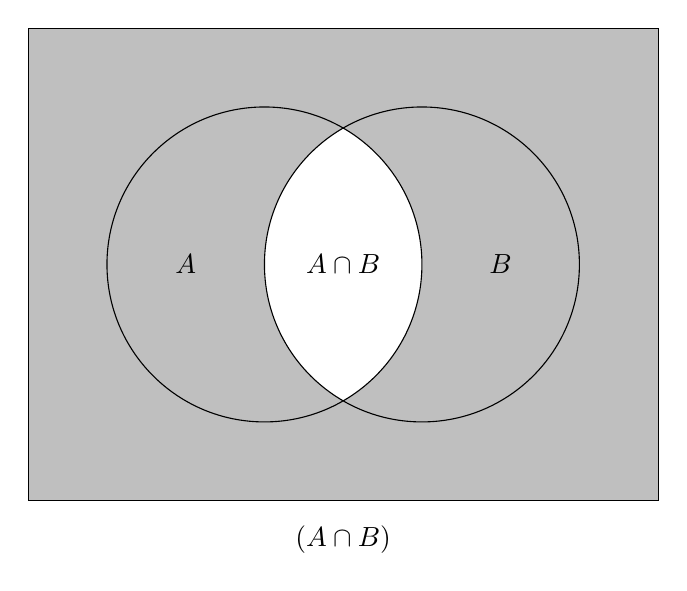
\begin{tikzpicture}
                \filldraw[fill=gray!50] (-3, -3) rectangle (5, 3);
                \scope
                \clip (0, 0) circle (2);
                \fill[white] (2, 0) circle (2);
                \endscope
                \draw (0, 0) circle (2)
                      (2, 0) circle (2);
                \node at (-1, 0) {\( A \)};
                \node at (1, 0) {\( A \cap B \)};
                \node at (3, 0) {\( B \)};
                \node at (1, -3.5) {\( \setcomp{(A \cap B)} \)};
            \end{tikzpicture}
            \hspace{4mm}
            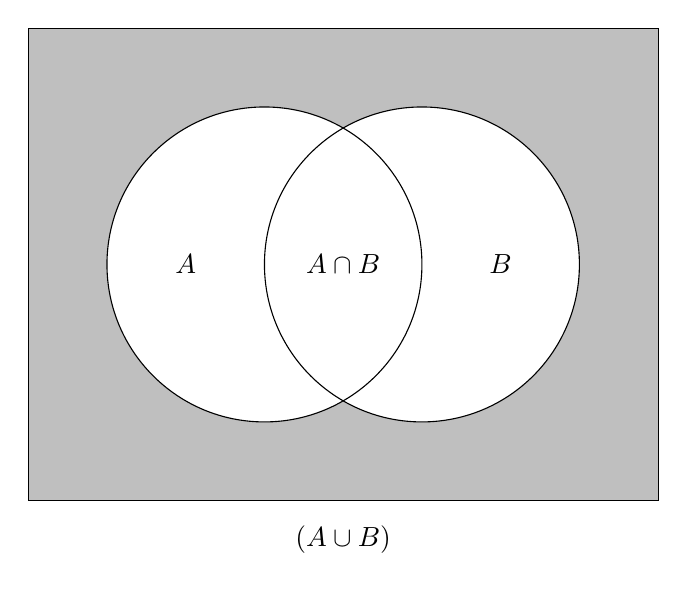
\begin{tikzpicture}
                \filldraw[fill=gray!50] (-3, -3) rectangle (5, 3);
                \fill[fill=white] (2, 0) circle (2);
                \filldraw[fill=white, draw=black] (0, 0) circle (2);
                \draw (2, 0) circle (2);
                \node at (-1, 0) {\( A \)};
                \node at (1, 0) {\( A \cap B \)};
                \node at (3, 0) {\( B \)};
                \node at (1, -3.5) {\( \setcomp{(A \cup B)} \)};
            \end{tikzpicture}
            \\[4mm]
            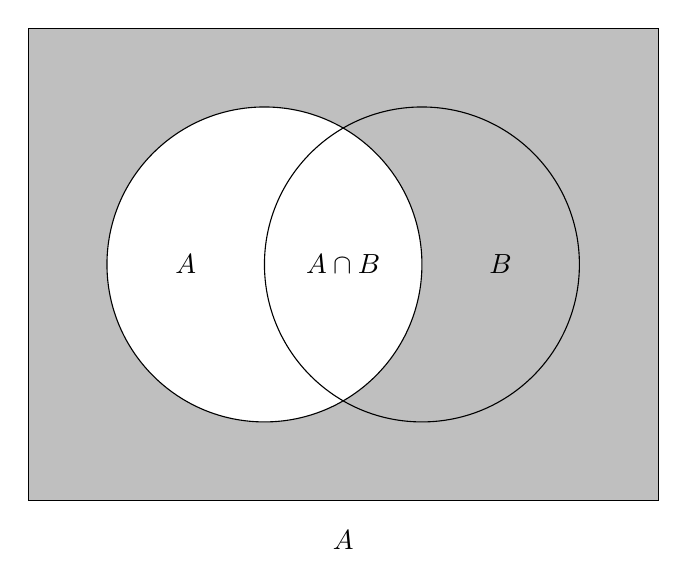
\begin{tikzpicture}
                \filldraw[fill=gray!50] (-3, -3) rectangle (5, 3);
                \filldraw[fill=white, draw=black] (0, 0) circle (2);
                \draw (2, 0) circle (2);
                \node at (-1, 0) {\( A \)};
                \node at (1, 0) {\( A \cap B \)};
                \node at (3, 0) {\( B \)};
                \node at (1, -3.5) {\( \setcomp{A} \)};
            \end{tikzpicture}
            \hspace{4mm}
            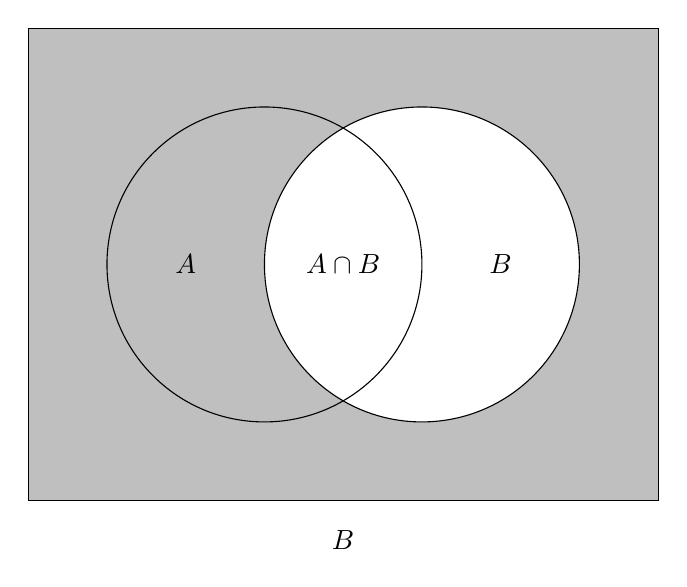
\begin{tikzpicture}
                \filldraw[fill=gray!50] (-3, -3) rectangle (5, 3);
                \filldraw[fill=white, draw=black] (2, 0) circle (2);
                \draw (0, 0) circle (2);
                \node at (-1, 0) {\( A \)};
                \node at (1, 0) {\( A \cap B \)};
                \node at (3, 0) {\( B \)};
                \node at (1, -3.5) {\( \setcomp{B} \)};
            \end{tikzpicture}
            \caption{Venn diagram for De Morgan's Laws; shaded regions are included, white regions are excluded }
            \label{fig:ex1.2.5}
        \end{figure}

        \item See part (a). \Cref{fig:ex1.2.5} shows some Venn diagrams which help to visualize De Morgan's Laws.

        \item The proof is similar to the one given in parts (a) and (b):
        \begin{multline*}
            x \in \setcomp{(A \cup B)} \iff x \not\in A \cup B \iff \text{not } (x \in A \text{ or } x \in B) \\[2mm]
            \iff x \not\in A \text{ and } x \not\in B \iff x \in \setcomp{A} \cap \setcomp{B}.
        \end{multline*}
    \end{enumerate}
\end{solution}

\begin{exercise}
\label{ex:1.2.6}
    \begin{enumerate}
        \item Verify the triangle inequality in the special case where \( a \) and \( b \) have the same sign.

        \item Find an efficient proof for all the cases at once by first demonstrating \( (a + b)^2 \leq (\abs{a} + \abs{b})^2 \).

        \item Prove \( \abs{a - b} \leq \abs{a - c} + \abs{c - d} + \abs{d - b} \) for all \( a, b, c, \) and \( d \).

        \item Prove \( \abs{\abs{a} - \abs{b}} \leq \abs{a - b} \). (The unremarkable identity \( a = a - b + b \) may be useful.)
    \end{enumerate}
\end{exercise}

\begin{solution}
    \begin{enumerate}
        \item First suppose that \( a \) and \( b \) are both non-negative, so that \( a + b \) is also non-negative; it follows that \( \abs{a + b} = a + b \) and \( \abs{a} + \abs{b} = a + b \). Thus the triangle inequality in this case reduces to the evidently true statement \( a + b \leq a + b \).

        Now suppose that \( a \) and \( b \) are both negative, so that \( a + b \) is also negative; it follows that \( \abs{a + b} = -a - b \) and \( \abs{a} + \abs{b} = -a - b \). Thus the triangle inequality in this case reduces to the evidently true statement \( -a - b \leq -a - b \).

        \item Starting from the true statement \( ab \leq \abs{ab} \) and using that \( a^2 = \abs{a}^2 \) and \( \abs{ab} = \abs{a} \abs{b} \) for any real numbers \( a \) and \( b \), observe that
        \begin{multline*}
            2ab \leq 2 \abs{ab} \iff a^2 + 2ab + b^2 \leq \abs{a}^2 + 2 \abs{a} \abs{b} + \abs{b}^2 \\[2mm]
            \iff (a + b)^2 \leq (\abs{a} + \abs{b})^2 \iff \abs{a + b}^2 \leq (\abs{a} + \abs{b})^2.
        \end{multline*}
        Because both \( \abs{a + b} \) and \( \abs{a} + \abs{b} \) are non-negative, the inequality \( \abs{a + b}^2 \leq (\abs{a} + \abs{b})^2\) is equivalent to \( \abs{a + b} \leq \abs{a} + \abs{b} \), as desired.

        \item We apply the triangle inequality twice:
        \[
            \abs{a - b} = \abs{a - c + c - b} \leq \abs{a - c} + \abs{c - b} \leq \abs{a - c} + \abs{c - d} + \abs{d - b}.
        \]

        \item Using the triangle inequality and the fact that \( \abs{-a} = \abs{a} \) for any \( a \in \R \), we find that
        \begin{gather*}
            \abs{a} = \abs{a - b + b} \leq \abs{a - b} + \abs{b} \iff \abs{a} - \abs{b} \leq \abs{a - b}, \\[2mm]
            \abs{b} = \abs{b - a + a} \leq \abs{b - a} + \abs{a} = \abs{a - b} + \abs{a} \iff \abs{b} - \abs{a} \leq \abs{a - b}.
        \end{gather*}
        Since \( \abs{\abs{a} - \abs{b}} \) equals either \( \abs{a} - \abs{b} \) or \( \abs{b} - \abs{a} \), it follows that \( \abs{\abs{a} - \abs{b}} \leq \abs{a - b} \).
    \end{enumerate}
\end{solution}

\begin{exercise}
\label{ex:1.2.7}
    Given a function \( f \) and a subset \( A \) of its domain, let \( f(A) \) represent the range of \( f \) over the set \( A \); that is, \( f(A) = \{ f(x) : x \in A \} \).
    \begin{enumerate}
        \item Let \( f(x) = x^2 \). If \( A = [0, 2] \) (the closed interval \( \{ x \in \R : 0 \leq x \leq 2 \} \)) and \( B = [1, 4] \), find \( f(A) \) and \( f(B) \). Does \( f(A \cap B) = f(A) \cap f(B) \) in this case? Does \( f(A \cup B) = f(A) \cup f(B) \)?

        \item Find two sets \( A \) and \( B \) for which \( f(A \cap B) \neq f(A) \cap f(B) \).

        \item Show that, for an arbitrary function \( g : \R \to \R \), it is always true that \( g(A \cap B) \subseteq g(A) \cap g(B) \) for all sets \( A, B \subseteq \R \).

        \item Form and prove a conjecture about the relationship between \( g(A \cup B) \) and \( g(A) \cup g(B) \) for an arbitrary function \( g \).
    \end{enumerate}
\end{exercise}

\begin{solution}
    \begin{enumerate}
        \item Some straightforward calculations reveal that
        \[
            \begin{gathered}
                f(A) = [0, 4], \\[2mm]
                f(B) = [1, 16],
            \end{gathered}
            \hspace{10mm}
            \begin{gathered}
                f(A \cap B) = f([1, 2]) = [1, 4], \\[2mm]
                f(A) \cap f(B) = [1, 4],
            \end{gathered}
            \hspace{10mm}
            \begin{gathered}
                f(A \cup B) = f([0, 4]) = [0, 16], \\[2mm]
                f(A) \cup f(B) = [0, 16].
            \end{gathered}
        \]
        From this we see that \( f(A \cap B) = f(A) \cap f(B) \) and \( f(A \cup B) = f(A) \cup f(B) \).
    
        \item Let \( A = \{ -1 \} \) and \( B = \{ 1 \} \). Then \( f(A \cap B) = f(\emptyset) = \emptyset \) but
        \[
            f(A) \cap f(B) = \{ 1 \} \cap \{ 1 \} = \{ 1 \} \neq \emptyset.
        \]

        \item Observe that
        \begin{gather*}
            y \in g(A \cap B) \iff y = g(x) \text{ for some } x \in A \cap B \\[2mm]
            \implies (y = g(x_1) \text{ for some } x_1 \in A) \text{ and } (y = g(x_2) \text{ for some } x_2 \in B) \\[2mm]
            \iff y \in g(A) \text{ and } y \in g(B) \iff y \in g(A) \cap g(B).
        \end{gather*}
        It follows that \( y \) belongs to \( g(A) \cap g(B) \) whenever \( y \) belongs to \( g(A \cap B) \), which is to say that \( g(A \cap B) \subseteq g(A) \cap g(B) \).

        \item We always have \( g(A \cup B) = g(A) \cup g(B) \); indeed,
        \begin{gather*}
            y \in g(A \cup B) \iff y = g(x) \text{ for some } x \in A \cup B \\[2mm]
            \iff y = g(x) \text{ for some } x \text{ such that } (x \in A \text{ or } x \in B) \\[2mm]
            \iff (y = g(x_1) \text{ for some } x_1 \in A) \text{ or } (y = g(x_2) \text{ for some } x_2 \in B) \\[2mm]
            \iff y \in g(A) \text{ or } y \in g(B) \iff y \in g(A) \cup g(B).
        \end{gather*}
        It follows that \( g(A \cup B) = g(A) \cup g(B) \).
    \end{enumerate}
\end{solution}

\begin{exercise}
\label{ex:1.2.8}
    Here are two important definitions related to a function \( f : A \to B \). The function \( f \) is \textit{one-to-one} (1-1) if \( a_1 \neq a_2 \) in \( A \) implies that \( f(a_1) \neq f(a_2) \) in \( B \). The function \( f \) is \textit{onto} if, given any \( b \in B \), it is possible to find an element \( a \in A \) for which \( f(a) = b \).

    Give an example of each or state that the request is impossible:
    \begin{enumerate}
        \item \( f : \N \to \N \) that is 1-1 but not onto.

        \item \( f : \N \to \N \) that is onto but not 1-1.

        \item \( f : \N \to \Z \) that is 1-1 and onto.
    \end{enumerate}
\end{exercise}

\begin{solution}
    (I prefer the terms injective/surjective/bijective rather than one-to-one and onto; see \hyperlink{notation}{notation}. I will use these terms throughout this document.)
    \begin{enumerate}
        \item Let \( f : \N \to \N \) be given by \( f(n) = 2n \). Then \( f \) is injective since \( n = m \) if and only if \( 2n = 2m \), but \( f \) is not surjective since the range of \( f \) contains only even numbers.
        \[
            \begin{tikzcd}[row sep = 12mm, column sep = 4mm]
                \N \arrow[d, "f" {left, font=\normalsize}] & 1 \arrow[rd] & 2 \arrow[rrd] & 3 \arrow[rrrd] & \cdots \\
                \N & 1 & 2 & 3 & 4 & 5 & 6 & \cdots
            \end{tikzcd}
        \]

        \item Let \( f : \N \to \N \) be given by \( f(1) = 1 \) and \( f(n) = n - 1 \) for \( n \geq 2 \). Then \( f(n + 1) = n \) for any \( n \in \N \), so that \( f \) is surjective, but \( f \) is not injective since \( f(1) = f(2) = 1 \).
        \[
            \begin{tikzcd}[row sep = 12mm, column sep = 4mm]
                \N \arrow[d, "f" {left, font=\normalsize}] & 1 \arrow[d] & 2 \arrow[ld] & 3 \arrow[ld] & 4 \arrow[ld] & 5 \arrow[ld] & \cdots \\
                \N & 1 & 2 & 3 & 4 & \cdots
            \end{tikzcd}
        \]

        \item Let \( f : \N \to \Z \) be given by
        \[
            f(n) = \begin{cases}
                \tfrac{n}{2} & \text{if } n \text{ is even}, \\
                -\tfrac{n-1}{2} & \text{if } n \text{ is odd}.
            \end{cases}
        \]
        \[
            \begin{tikzcd}[row sep = 12mm, column sep = 4mm]
                \N \arrow[d, "f" {left, font=\normalsize}] & 1 \arrow[d] & 2 \arrow[d] & 3 \arrow[d] & 4 \arrow[d] & 5 \arrow[d] & \cdots \\
                \Z & 0 & 1 & -1 & 2 & -2 & \cdots
            \end{tikzcd}
        \]
        To see that \( f \) is injective, let \( n \neq m \) be given and consider these cases.
        \begin{description}
            \item[Case 1.] If \( n \) and \( m \) are both even, then \( f(n) \neq f(m) \) since \( n \neq m \) if and only if \( \tfrac{n}{2} \neq \tfrac{m}{2} \).

            \item[Case 2.] If \( n \) and \( m \) are both odd, then \( f(n) \neq f(m) \) since \( n \neq m \) if and only if \( -\tfrac{n-1}{2} \neq -\tfrac{m-1}{2} \).

            \item[Case 3.] If \( n \) and \( m \) have opposite signs, say \( n \) is even and \( m \) is odd, then \( f(n) \neq f(m) \) since \( f(n) > 0 \) and \( f(m) \leq 0 \).
        \end{description}
        To see that \( f \) is surjective, let \( n \in \Z \) be given. If \( n > 0 \), then \( f(2n) = n \), and if \( n \leq 0 \) then \( f(-2n + 1) = n \).
    \end{enumerate}
\end{solution}

\begin{exercise}
\label{ex:1.2.9}
    Given a function \( f : D \to \R \) and a subset \( B \subseteq \R \), let \( f^{-1}(B) \) be the set of all points from the domain \( D \) that get mapped into \( B \); that is, \( f^{-1}(B) = \{ x \in D : f(x) \in B \} \). This set is called the \textit{preimage} of \( B \).
    \begin{enumerate}
        \item Let \( f(x) = x^2 \). If \( A \) is the closed interval \( [0, 4] \) and \( B \) is the closed interval \( [-1, 1] \), find \( f^{-1}(A) \) and \( f^{-1}(B) \). Does \( f^{-1}(A \cap B) = f^{-1}(A) \cap f^{-1}(B) \) in this case? Does \( f^{-1}(A \cup B) = f^{-1}(A) \cup f^{-1}(B) \)?

        \item The good behavior of preimages demonstrated in (a) is completely general. Show that for an arbitrary function \( g : \R \to \R \), it is always true that \( g^{-1}(A \cap B) = g^{-1}(A) \cap g^{-1}(B) \) and \( g^{-1}(A \cup B) = g^{-1}(A) \cup g^{-1}(B) \) for all sets \( A, B \subseteq \R \).
    \end{enumerate}
\end{exercise}

\begin{solution}
    \begin{enumerate}
        \item Some straightforward calculations reveal that
        \[
            \begin{gathered}
                f^{-1}(A) = [-2, 2], \\[2mm]
                f^{-1}(B) = [-1, 1],
            \end{gathered}
            \hspace{10mm}
            \begin{gathered}
                f^{-1}(A \cap B) = [-1, 1], \\[2mm]
                f^{-1}(A) \cap f^{-1}(B) = [-1, 1],
            \end{gathered}
            \hspace{10mm}
            \begin{gathered}
                f^{-1}(A \cup B) = [-2, 2], \\[2mm]
                f^{-1}(A) \cup f^{-1}(B) = [-2, 2].
            \end{gathered}
        \]
        From this we see that \( f^{-1}(A \cap B) = f^{-1}(A) \cap f^{-1}(B) \) and \( f^{-1}(A \cup B) = f^{-1}(A) \cup f^{-1}(B) \).

        \item Observe that
        \begin{gather*}
            x \in g^{-1}(A \cap B) \iff g(x) \in A \cap B \iff (g(x) \in A) \text{ and } (g(x) \in B) \\[2mm]
            \iff (x \in g^{-1}(A)) \text{ and } (x \in g^{-1}(B)) \iff x \in g^{-1}(A) \cap g^{-1}(B).
        \end{gather*}
        Similarly,
        \begin{gather*}
            x \in g^{-1}(A \cup B) \iff g(x) \in A \cup B \iff (g(x) \in A) \text{ or } (g(x) \in B) \\[2mm]
            \iff (x \in g^{-1}(A)) \text{ or } (x \in g^{-1}(B)) \iff x \in g^{-1}(A) \cup g^{-1}(B).
        \end{gather*}
    \end{enumerate}
\end{solution}

\begin{exercise}
\label{ex:1.2.10}
    Decide which of the following are true statements. Provide a short justification for those that are valid and a counterexample for those that are not:
    \begin{enumerate}
        \item Two real numbers satisfy \( a < b \) if and only if \( a < b + \epsilon \) for every \( \epsilon > 0 \).

        \item Two real numbers satisfy \( a < b \) if \( a < b + \epsilon \) for every \( \epsilon > 0 \).

        \item Two real numbers satisfy \( a \leq b \) if and only if \( a < b + \epsilon \) for every \( \epsilon > 0 \).
    \end{enumerate}
\end{exercise}

\begin{solution}
    \begin{enumerate}
        \item This is false; the implication
        \begin{center}
            if \( a < b + \epsilon \) for every \( \epsilon > 0 \), then \( a < b \)
        \end{center}
        does not hold. The problem occurs when we consider the case where \( a = b \). For example, we certainly have \( 1 < 1 + \epsilon \) for every \( \epsilon > 0 \) but of course \( 1 < 1 \) is false.

        \item See part (a).

        \item This is true. The implication
        \begin{center}
            if \( a \leq b \), then \( a < b + \epsilon \) for every \( \epsilon > 0 \)
        \end{center}
        follows since \( a \leq b < b + \epsilon \) for every \( \epsilon > 0 \) and the implication
        \begin{center}
            if \( a > b \), then \( a \geq b + \epsilon \) for some \( \epsilon > 0 \)
        \end{center}
        can be seen by taking \( \epsilon = a - b > 0 \), so that \( b + \epsilon = a \leq a \).
    \end{enumerate}
\end{solution}

\begin{exercise}
\label{ex:1.2.11}
    Form the logical negation of each claim. One trivial way to do this is to simply add ``It is not the case that..." in front of each assertion. To make this interesting, fashion the negation into a positive statement that avoids using the word ``not" altogether. In each case, make an intuitive guess as to whether the claim or its negation is the true statement.
    \begin{enumerate}
        \item For all real numbers satisfying \( a < b \), there exists an \( n \in \N \) such that \( a + 1/n < b \).

        \item There exists a real number \( x > 0 \) such that \( x < 1/n \) for all \( n \in \N \).

        \item Between every two distinct real numbers there is a rational number.
    \end{enumerate}
\end{exercise}

\begin{solution}
    \begin{enumerate}
        \item The negated statement is:
        \begin{center}
            there exist real numbers \( a < b \) such that \( a + \tfrac{1}{n} \geq b \) for all \( n \in \N \).
        \end{center}
        The original statement is true and follows from the Archimedean Property (Theorem 1.4.2).

        \item The negated statement is:
        \begin{center}
            for all \( x > 0 \), there exists an \( n \in \N \) such that \( \tfrac{1}{n} \leq x \).
        \end{center}
        The negated statement is true and again follows from the Archimedean Property (Theorem 1.4.2).

        \item The negated statement is:
        \begin{center}
            there are two distinct real numbers with no rational number between them.
        \end{center}
        The original statement is true; this is the density of \( \Q \) in \( \R \) (Theorem 1.4.3).
    \end{enumerate}
\end{solution}

\begin{exercise}
\label{ex:1.2.12}
    Let \( y_1 = 6 \), and for each \( n \in \N \) define \( y_{n+1} = (2y_n - 6)/3 \).
    \begin{enumerate}
        \item Use induction to prove that the sequence satisfies \( y_n > -6 \) for all \( n \in \N \).

        \item Use another induction argument to show the sequence \( (y_1, y_2, y_3, \ldots) \) is decreasing.
    \end{enumerate}
\end{exercise}

\begin{solution}
    \begin{enumerate}
        \item For \( n \in \N \), let \( P(n) \) be the statement that \( y_n > -6 \). Since \( y_1 = 6 \), the truth of \( P(1) \) is clear. Suppose that \( P(n) \) holds for some \( n \in \N \) and observe that
        \[
            y_{n+1} = \frac{2}{3} y_n - 2 > \frac{2}{3} (-6) - 2 = -6,
        \]
        i.e., \( P(n + 1) \) holds. This completes the induction step and we may conclude that \( P(n) \) holds for all \( n \in \N \).

        \item For \( n \in \N \), let \( P(n) \) be the statement that \( y_{n+1} \leq y_n \). Since \( y_1 = 6 \) and \( y_2 = 2 \), the truth of \( P(1) \) is clear. Suppose that \( P(n) \) holds for some \( n \in \N \) and observe that
        \[
            y_{n+2} = \frac{2}{3} y_{n+1} - 2 \leq \frac{2}{3} y_n - 2 = y_{n+1},
        \]
        i.e., \( P(n + 1) \) holds. This completes the induction step and we may conclude that \( P(n) \) holds for all \( n \in \N \).
    \end{enumerate}
\end{solution}

\begin{exercise}
\label{ex:1.2.13}
    For this exercise, assume \Cref{ex:1.2.5} has been successfully completed.
    \begin{enumerate}
        \item Show how induction can be used to conclude that
        \[
            \setcomp{(A_1 \cup A_2 \cup \cdots \cup A_n)} = \setcomp{A_1} \cap \setcomp{A_2} \cap \cdots \cap \setcomp{A_n}
        \]
        for any finite \( n \in \N \).

        \item It is tempting to appeal to induction to conclude that
        \[
            \setcomp{\paren{ \bigcup_{i=1}^{\infty} A_i }} = \bigcap_{i=1}^{\infty} \setcomp{A_i},
        \]
        but induction does not apply here. Induction is used to prove that a particular statement holds for every value of \( n \in \N \), but this does not imply the validity of the infinite case. To illustrate this point, find an example of a collection of sets \( B_1, B_2, B_3, \ldots \) where \( \bigcap_{i=1}^n B_i \neq \emptyset \) is true for every \( n \in \N \), but \( \bigcap_{i=1}^{\infty} B_i \neq \emptyset \) fails.

        \item Nevertheless, the infinite version of De Morgan's Law stated in (b) is a valid statement. Provide a proof that does not use induction.
    \end{enumerate}
\end{exercise}

\begin{solution}
    \begin{enumerate}
        \item For \( n \in \N \), let \( P(n) \) be the statement that \( \setcomp{(A_1 \cup \cdots \cup A_n)} = \setcomp{A_1} \cap \cdots \cap \setcomp{A_n} \) for any sets \( A_1, \ldots, A_n \). The truth of \( P(1) \) is clear. Suppose that \( P(n) \) holds for some \( n \in \N \), let \( A_1, \ldots, A_n, A_{n+1} \) be given, and observe that
        \begin{align*}
            \setcomp{(A_1 \cup \cdots \cup A_n \cup A_{n+1})} &= \setcomp{((A_1 \cup \cdots \cup A_n) \cup (A_{n+1}))} \\[2mm]
            &= \setcomp{(A_1 \cup \cdots \cup A_n)} \cap \setcomp{A_{n+1}} \tag{\Cref{ex:1.2.5}} \\[2mm]
            &= \setcomp{A_1} \cap \cdots \cap \setcomp{A_n} \cap \setcomp{A_{n+1}}, \tag{induction hypothesis}
        \end{align*}
        i.e., \( P(n + 1) \) holds. This completes the induction step and we may conclude that \( P(n) \) holds for all \( n \in \N \).

        \item Let \( B_i = \{ i, i + 1, i + 2, \ldots \} \), so that
        \[
            B_1 = \{ 1, 2, 3, \ldots \}, \hspace{4mm} B_2 = \{ 2, 3, 4, \ldots \}, \hspace{4mm} B_3 = \{ 3, 4, 5, \ldots \}, \hspace{4mm} \text{ etc}.
        \]
        It is straightforward to verify that \( \bigcap_{i=1}^n B_i = B_n \neq \emptyset \) for any \( n \in \N \); however, as Example 1.2.2 shows, the intersection \( \bigcap_{i=1}^{\infty} B_i \) is empty.

        \item Observe that
        \[
            x \in \setcomp{\paren{ \bigcup_{i=1}^{\infty} A_i }} \iff x \not\in \bigcup_{i=1}^{\infty} A_i \iff x \not\in A_i \text{ for every } i \in \N \iff x \in \bigcap_{i=1}^{\infty} \setcomp{A_i}.
        \]
        It follows that
        \[
            \setcomp{\paren{ \bigcup_{i=1}^{\infty} A_i }} = \bigcap_{i=1}^{\infty} \setcomp{A_i}.
        \]
    \end{enumerate}
\end{solution}

\section{The Axiom of Completeness}
\label{sec:1.3}

\begin{exercise}
\label{ex:1.3.1}
    \begin{enumerate}
        \item Write a formal definition in the style of Definition 1.3.2 for the \textit{infimum} or \textit{greatest lower bound} of a set.

        \item Now, state and prove a version of Lemma 1.3.8 for greatest lower bounds.
    \end{enumerate}
\end{exercise}

\begin{solution}
    \begin{enumerate}
        \item A real number \( t \) is the \textit{greatest lower bound} for a set \( A \subseteq \R \) if it meets the following two criteria:
        \begin{enumerate}[label = (\roman*)]
            \item \( t \) is a lower bound for \( A \);

            \item if \( b \) is any lower bound for \( A \), then \( b \leq t \).
        \end{enumerate}

        \item Here is a version of Lemma 1.3.8 for greatest lower bounds.
        \begin{lemma}
        \label{lem:ex1.3.1}
            Assume \( t \in \R \) is a lower bound for a set \( A \subseteq \R \). Then \( t = \inf A \) if and only if, for every choice of \( \epsilon > 0 \), there exists an element \( a \in A \) satisfying \( a < t + \epsilon \).
        \end{lemma}

        \begin{proof}
            First, let us prove the implication
            \begin{center}
                if \( t = \inf A \), then for every \( \epsilon > 0 \) there exists an \( a \in A \) such that \( a < t + \epsilon \)
            \end{center}
            by proving the contrapositive statement
            \begin{center}
                if there exists an \( \epsilon > 0 \) such that \( t + \epsilon \leq a \) for every \( a \in A \) then \( t \neq \inf A \).
            \end{center}
            If such an \( \epsilon > 0 \) exists, then \( t + \epsilon \) is a lower bound for \( A \) strictly greater than \( t \); it follows that \( t \) is not the greatest lower bound for \( A \), i.e., \( t \neq \inf A \).

            Now let us prove the converse:
            \begin{center}
                if for every \( \epsilon > 0 \) there exists an \( a \in A \) such that \( a < t + \epsilon \), then \( t = \inf A \).
            \end{center}
            Suppose \( b \in \R \) is such that \( b > t \). Taking \( \epsilon = b - t > 0 \), by assumption we are guaranteed the existence of an \( a \in A \) such that \( a < t + \epsilon = b \). Thus \( b \) is not a lower bound for \( A \); this proves the contrapositive of criterion (ii) in part (a) and we may conclude that \( t = \inf A \).
        \end{proof}
    \end{enumerate}
\end{solution}

\begin{exercise}
\label{ex:1.3.2}
    Give an example of each of the following, or state that the request is impossible.
    \begin{enumerate}
        \item A set \( B \) with \( \inf B \geq \sup B \).

        \item A finite set that contains its infimum but not its supremum.

        \item A bounded subset of \( \Q \) that contains its supremum but not its infimum.
    \end{enumerate}
\end{exercise}

\begin{solution}
    \begin{enumerate}
        \item Take \( B = \{ 0 \} \), so that \( \inf B = \sup B = 0 \).

        \item This is impossible. To see this, let us first use induction to show that any non-empty finite subset of \( \R \) contains a minimum and a maximum element.
        \begin{lemma}
        \label{lem:ex1.3.2}
            If \( E \subseteq \R \) is non-empty and finite, then \( E \) contains a minimum and a maximum element.
        \end{lemma}

        \begin{proof}
            For \( n \in \N \), let \( P(n) \) be the statement that any subset of \( \R \) containing \( n \) elements has a minimum and a maximum element. For the base case \( P(1) \), simply observe that \( \min \{ x \} = \max \{ x \} = x \) for any \( x \in \R \).

            Suppose that \( P(n) \) holds for some \( n \in \N \) and let \( E \subseteq \R \) be a set containing \( n + 1 \) elements. Fix some \( x \in E \) and consider the set \( F = E \setminus \{ x \} \), which contains \( n \) elements. Our induction hypothesis guarantees the existence of a minimum element \( a := \min F \) and a maximum element \( b := \max F \), which must satisfy \( a \leq b \). There are then three cases; the conclusion in each case is straightforward to verify.
            \begin{description}
                \item[Case 1.] If \( x < a \), then \( \min E = x \) and \( \max E = b \).

                \item[Case 2.] If \( x > b \), then \( \min E = a \) and \( \max E = x \).

                \item[Case 3.] If \( a \leq x \leq b \), then \( \min E = a \) and \( \max E = b \).
            \end{description}
            In any case, the set \( E \) has a minimum and a maximum element, i.e., \( P(n + 1) \) holds. This completes the induction step and the proof.
        \end{proof}
        It is immediate from the definition of the supremum and the maximum of a set \( E \subseteq \R \) that if \( \max E \) exists then \( \sup E = \max E \) (see \Cref{ex:1.3.7}); similarly, if \( \min E \) exists then \( \inf E = \min E \). It follows that the given request is impossible: if \( E \subseteq \R \) is finite, then \Cref{lem:ex1.3.2} implies that \( \min E = \inf E \) and \( \max E = \sup E \) both exist and hence \( E \) contains both its infimum and its supremum.

        \item Consider the bounded set \( E = \{ p \in \Q : 0 < p \leq 1 \} \), which satisfies \( \sup E = 1 \in E \) and \( \inf E = 0 \not\in E \).
    \end{enumerate}
\end{solution}

\begin{exercise}
\label{ex:1.3.3}
    \begin{enumerate}
        \item Let \( A \) be nonempty and bounded below, and define \( B = \{ b \in \R : b \) is a lower bound for \( A \} \). Show that \( \sup B = \inf A \).

        \item Use (a) to explain why there is no need to assert that greatest lower bounds exist as part of the Axiom of Completeness.
    \end{enumerate}
\end{exercise}

\begin{solution}
    \begin{enumerate}
        \item \( B \) is non-empty since \( A \) is bounded below, and \( B \) is bounded above by any \( x \in A \); there exists at least one such \( x \) since \( A \) is non-empty. It follows from the Axiom of Completeness that \( \sup B \) exists. To see that \( \sup B = \inf A \), we need to show that \( \sup B \) satisfies criteria (i) and (ii) from \Cref{ex:1.3.1} (a).
        \begin{enumerate}[label = (\roman*)]
            \item First we need to prove that \( \sup B \) is a lower bound for \( A \), i.e., if \( x \in A \), then \( \sup B \leq x \). We will prove the contrapositive statement: if \( x < \sup B \), then \( x \not\in A \). If \( x \) is strictly less than \( \sup B \), then \( x \) cannot be an upper bound for \( B \). Thus there exists some \( b \in B \) such that \( x < b \). Since \( b \) is a lower bound for \( A \), it follows that \( x \not\in A \).
    
            \item Suppose \( y \in \R \) is a lower bound of \( A \), so that \( y \) belongs to \( B \); it follows that \( y \leq \sup B \).
        \end{enumerate}
        We may conclude that \( \sup B = \inf A \).

        \item Part (a) shows that the existence of the greatest lower bound for non-empty bounded below subsets of \( \R \) is implied by the Axiom of Completeness; adding this existence as part of the Axiom of Completeness would be redundant.
    \end{enumerate}
\end{solution}

\begin{exercise}
\label{ex:1.3.4}
    Let \( A_1, A_2, A_3, \ldots \) be a collection of nonempty sets, each of which is bounded above.
    \begin{enumerate}
        \item Find a formula for \( \sup (A_1 \cup A_2) \). Extend this to \( \sup \paren{ \bigcup_{k=1}^n A_k } \).

        \item Consider \( \sup \paren{ \bigcup_{k=1}^{\infty} A_k } \). Does the formula in (a) extend to the infinite case?
    \end{enumerate}
\end{exercise}

\begin{solution}
    \begin{enumerate}
        \item Let \( n \in \N \) be given. For each \( k \in \{ 1, \ldots, n \} \), the Axiom of Completeness guarantees that \( \sup A_k \) exists. By \Cref{lem:ex1.3.2}, the finite set \( \{ \sup A_1, \ldots, \sup A_k \} \) has a maximum element, say \( M \); we claim that \( \sup \paren{ \bigcup_{k=1}^n A_k } = M \). To prove this, we must verify criteria (i) and (ii) from Definition 1.3.2.
        \begin{enumerate}[label=(\roman*)]
            \item If \( x \in \bigcup_{k=1}^n A_k \), then \( x \in A_k \) for some \( k \in \{ 1, \ldots, n \} \); it follows that \( x \leq \sup A_k \leq M \). Since \( x \) was arbitrary, we see that \( M \) is an upper bound for \( \bigcup_{k=1}^n A_k \).

            \item If \( b \in \R \) is an upper bound for \( \bigcup_{k=1}^n A_k \), then \( b \) must be an upper bound for each \( A_k \). It follows that \( \sup A_k \leq b \) for each \( k \in \{ 1, \ldots, n \} \) and hence that \( M \leq b \).
        \end{enumerate}
        We may conclude that \( \sup \paren{ \bigcup_{k=1}^n A_k } = M \).

        \item The proof given above does not extend to the infinite case, since in general the set \( \{ \sup A_1, \sup A_2, \ldots \} \) need not have a maximum. Indeed, it may be the case that \( \sup \paren{ \bigcup_{k=1}^{\infty} A_k } \) does not exist. For example, take \( A_k = [0, k] \). Then each \( A_k \) is non-empty and bounded above with \( \sup A_k = k \), but \( \bigcup_{k=1}^{\infty} A_k = [0, \infty) \), which does not have a supremum in \( \R \).
    \end{enumerate}
\end{solution}

\begin{exercise}
\label{ex:1.3.5}
    As in Example 1.3.7, let \( A \subseteq \R \) be nonempty and bounded above, and let \( c \in \R \). This time define the set \( cA = \{ ca : a \in A \} \).
    \begin{enumerate}
        \item If \( c \geq 0 \), show that \( \sup (cA) = c \sup A \).

        \item Postulate a similar type of statement for \( \sup (cA) \) for the case \( c < 0 \).
    \end{enumerate}
\end{exercise}

\begin{solution}
    \begin{enumerate}
        \item If \( c = 0 \) then the result is clear, so suppose that \( c > 0 \). For any \( x \in A \), notice that
        \[
            x \leq \sup A \iff cx \leq c \sup A.
        \]
        This demonstrates that \( c \sup A \) is an upper bound for \( cA \). 
        
        Suppose \( b \in \R \) is an upper bound for \( cA \), i.e., \( cx \leq b \) for all \( x \in A \). Then \( x \leq c^{-1} b \) for all \( x \in A \), i.e., \( c^{-1} b \) is an upper bound for \( A \). It follows that \( \sup A \leq c^{-1} b \) and hence that \( c \sup A \leq b \). We may conclude that \( \sup (cA) = c \sup A \).

        \item If \( c < 0 \) and \( \inf A \) exists then \( \sup (cA) = c \inf A \). The proof is similar to part (a). For any \( x \in A \), we have
        \[
            \inf A \leq x \iff cx \leq c \inf A,
        \]
        so that \( c \inf A \) is an upper bound for \( cA \).
        
        Suppose \( b \in \R \) is an upper bound for \( cA \), i.e., \( cx \leq b \) for all \( x \in A \). Then \( c^{-1} b \leq x \) for all \( x \in A \), so that \( c^{-1} b \) is a lower bound for \( A \). It follows that \( c^{-1} b \leq \inf A \) and hence that \( c \inf A \leq b \). We may conclude that \( \sup (cA) = c \inf A \).

        If \( \inf A \) doesn't exist then \( \sup (cA) \) doesn't exist either, since for \( c < 0 \) the set \( A \) is bounded below if and only if \( c A \) is bounded above. For example, \( A = (-\infty, 0) \) and \( c = -1 \) gives \( cA = (0, \infty) \).
    \end{enumerate}
\end{solution}

\begin{exercise}
\label{ex:1.3.6}
    Given sets \( A \) and \( B \), define \( A + B = \{ a + b : a \in A \text{ and } b \in B \} \). Follow these steps to prove that if \( A \) and \( B \) are nonempty and bounded above then \( \sup (A + B) = \sup A + \sup B \).
    \begin{enumerate}
        \item Let \( s = \sup A \) and \( t = \sup B \). Show \( s + t \) is an upper bound for \( A + B \).

        \item Now let \( u \) be an arbitrary upper bound for \( A + B \), and temporarily fix \( a \in A \). Show \( t \leq u - a \).

        \item Finally, show \( \sup (A + B) = s + t \).

        \item Construct another proof of this same fact using Lemma 1.3.8.
    \end{enumerate}
\end{exercise}

\begin{solution}
    \begin{enumerate}
        \item For any \( a \in A \) and \( b \in B \) we have \( a \leq s \) and \( b \leq t \). It follows that \( a + b \leq s + t \) and thus \( s + t \) is an upper bound for \( A + B \).

        \item For any \( b \in B \) we have \( a + b \leq u \), which gives \( b \leq u - a \). This demonstrates that \( u - a \) is an upper bound for \( B \) and so it follows that \( t \leq u - a \).

        \item Part (b) implies that for any \( a \in A \) we have \( t \leq u - a \), which gives \( a \leq u - t \). This shows that \( u - t \) is an upper bound for \( A \) and it follows that \( s \leq u - t \), i.e., \( s + t \leq u \). Since \( u \) was an arbitrary upper bound for \( A + B \), we may conclude that
        \[
            \sup(A + B) = s + t = \sup A + \sup B.
        \]

        \item Let \( \epsilon > 0 \) be given. By Lemma 1.3.8, there exist elements \( a \in A \) and \( b \in B \) such that \( s - \tfrac{\epsilon}{2} < a \) and \( t - \tfrac{\epsilon}{2} < b \), which implies that \( s + t - \epsilon < a + b \). We showed in part (a) that \( s + t \) is an upper bound for \( A + B \), so we may invoke Lemma 1.3.8 to conclude that \( \sup(A + B) = \sup A + \sup B \).
    \end{enumerate}
\end{solution}

\begin{exercise}
\label{ex:1.3.7}
    Prove that if \( a \) is an upper bound for \( A \), and if \( a \) is also an element of \( A \), then it must be that \( a = \sup A \).
\end{exercise}

\begin{solution}
    Let \( b \in \R \) be an upper bound of \( A \). Since \( a \in A \), we must have \( a \leq b \); it follows that \( a = \sup A \).
\end{solution}

\begin{exercise}
\label{ex:1.3.8}
    Compute, without proofs, the suprema and infima (if they exist) of the following sets:
    \begin{enumerate}
        \item \( \{ m/n : m, n \in \N \text{ with } m < n \} \).

        \item \( \{ (-1)^m/n : m, n \in \N \} \).

        \item \( \{ n/(3n+1) : n \in \N \} \).

        \item \( \{ m/(m+n) : m, n \in \N \} \).
    \end{enumerate}
\end{exercise}

\begin{solution}
    \begin{enumerate}
        \item The supremum is 1 and the infimum is 0.

        \item The supremum is 1 and the infimum is \( -1 \).

        \item The supremum is \( \tfrac{1}{3} \) and the infimum is \( \tfrac{1}{4} \).

        \item The supremum is 1 and the infimum is 0.
    \end{enumerate}
\end{solution}

\begin{exercise}
\label{ex:1.3.9}
    \begin{enumerate}
        \item If \( \sup A < \sup B \), show that there exists an element \( b \in B \) that is an upper bound for \( A \).

        \item Give an example to show that this is not always the case if we only assume \( \sup A \leq \sup B \).
    \end{enumerate}
\end{exercise}

\begin{solution}
    \begin{enumerate}
        \item Let \( \epsilon = \sup B - \sup A > 0 \). By Lemma 1.3.8, there exists a \( b \in B \) such that \( \sup B - \epsilon = \sup A < b \). It follows that \( b \) is an upper bound for \( A \).

        \item Take \( A = B = (0, 1) \). Then \( \sup A = \sup B = 1 \), but no element of \( B \) is an upper bound for \( A \) (the interval \( (0, 1) \) has no maximum element).
    \end{enumerate}
\end{solution}

\begin{exercise}[Cut Property]
\label{ex:1.3.10}
    The \textit{Cut Property} of the real numbers is the following:

    If \( A \) and \( B \) are nonempty, disjoint sets with \( A \cup B = \R \) and \( a < b \) for all \( a \in A \) and \( b \in B \), then there exists \( c \in \R \) such that \( x \leq c \) whenever \( x \in A \) and \( x \geq c \) whenever \( x \in B \).
    \begin{enumerate}
        \item Use the Axiom of Completeness to prove the Cut Property.

        \item Show that the implication goes the other way; that is, assume \( \R \) possesses the Cut Property and let \( E \) be a nonempty set that is bounded above. Prove \( \sup E \) exists.

        \item The punchline of parts (a) and (b) is that the Cut Property could be used in place of the Axiom of Completeness as the fundamental axiom that distinguishes the real numbers from the rational numbers. To drive this point home, give a concrete example showing that the Cut Property is not a valid statement when \( \R \) is replaced by \( \Q \).
    \end{enumerate}
\end{exercise}

\begin{solution}
    \begin{enumerate}
        \item Suppose that \( A \) and \( B \) are non-empty disjoint subsets of \( \R \) such that \( A \cup B = \R \) and \( a < b \) for all \( a \in A \) and \( b \in B \). Notice that \( A \) is non-empty (by assumption) and bounded above (because \( B \) is non-empty); the Axiom of Completeness then implies that \( c := \sup A \) exists. It follows that \( x \leq c \) for all \( x \in A \) and, since each element of \( B \) is an upper bound for \( A \), we also have \( x \geq c \) for all \( x \in B \).

        \item Suppose that \( E \subseteq \R \) is non-empty and bounded above. Define
        \begin{gather*}
            A = \{ a \in \mathbf{R} : a \text{ is not an upper bound of } E \}, \\[2mm]
            B = \setcomp{A} = \{ b \in \mathbf{R} : b \text{ is an upper bound of } E \}.
        \end{gather*}
        Notice that \( B \) is non-empty as \( E \) is bounded above and \( A \) is non-empty because \( x - 1 \in A \) for any \( x \in E \); we are guaranteed the existence of at least one \( x \in E \) as \( E \) is non-empty. Furthermore, \( A \) and \( B \) are evidently disjoint and satisfy \( A \cup B = \R \).
        
        Let \( a \in A \) and \( b \in B \) be given. Since \( a \) is not an upper bound for \( E \) there exists some \( x \in E \) such that \( a < x \) and since \( b \) is an upper bound for \( E \), we must then have \( x \leq b \); it follows that \( a < b \). We may now invoke the Cut Property to obtain a \( c \in \R \) such that \( x \leq c \) for all \( x \in A \) and \( x \geq c \) for all \( x \in B \).

        We claim that \( c = \sup E \). Since \( A \cup B = \R \) and \( A \cap B = \emptyset \), exactly one of \( c \in A \) or \( c \in B \) holds. Suppose that \( c \in A \), i.e., \( c \) is not an upper bound of \( E \), which is the case if and only if there is some \( z \in E \) such that \( c < z \). Observe that \( y := \tfrac{c + z}{2} \) satisfies \( c < y < z \), so that \( y \in A \); but this contradicts the fact that \( x \leq c \) for all \( x \in A \).
        
        So it must be the case that \( c \in B \), i.e., \( c \) is an upper bound for \( E \). The Cut Property says that \( c \leq x \) for all \( x \in B \); in other words, \( c \) is less than all other upper bounds of \( E \). We may conclude that \( c = \sup E \).

        \item A concrete example is given in the following lemma, which will also be useful for later exercises.
        \begin{lemma}
        \label{lem:ex1.3.10}
            Let
            \[
                A = \{ p \in \Q : p < 0 \text{ or } p^2 < 2 \} \quad \text{and} \quad B = \{ p \in \Q : p > 0 \text{ and } p^2 > 2 \}.
            \]
            Then:
            \begin{enumerate}[label=(\roman*)]
                \item \( A \) and \( B \) are non-empty, \( A \cup B = \Q \), and \( A \cap B = \emptyset \).

                \item \( p < q \) for all \( p \in A \) and \( q \in B \).

                \item \( A \) has no maximum element and \( B \) has no minimum element.
            \end{enumerate}
        \end{lemma}

        \begin{proof}
            \begin{enumerate}[label=(\roman*)]
                \item It is clear that \( A \) and \( B \) are non-empty. The negation of the statement ``\( p < 0 \) or \( p^2 < 2 \)'' is ``\( p > 0 \) and \( p^2 \geq 2 \)''; by Theorem 1.1.1, this negated statement is equivalent to ``\( p > 0 \) and \( p^2 > 2 \)'' for \( p \in \Q \). Thus \( B = \Q \setminus A \), from which it follows that \( A \cup B = \Q \) and \( A \cap B = \emptyset \).

                \item Let \( p \in A \) and \( q \in B \) be given. If \( p \leq 0 \) then evidently \( p < q \), so suppose that \( p > 0 \). It must then be the case that \( p^2 < 2 \), whence \( p^2 < q^2 \). Since \( p \) and \( q \) are positive, this implies that \( p < q \).

                \item Let \( p \in A \) be given. We need to show that there exists some \( q \in A \) such that \( p < q \). If \( p \leq 0 \), we can take \( q = 1 \); if \( p > 0 \), so that \( p^2 < 2 \), then define
                \[
                    q = p + \frac{2 - p^2}{p + 2} = \frac{2p + 2}{p + 2}. \tag{1}
                \]
                Notice that \( 0 < \tfrac{2 - p^2}{p + 2} \), since \( p^2 < 2 \), from which it follows that \( p < q \). A straightforward calculation yields
                \[
                    2 - q^2 = \frac{2(2 - p^2)}{(p + 2)^2};
                \]
                using again that \( p^2 < 2 \), we see that \( 2 - q^2 > 0 \) and thus \( q \in A \).

                Now let \( p \in B \) be given. We need to show that there exists some \( q \in B \) such that \( q < p \). In fact, we can define \( q \) by equation (1) again; an argument similar to the one just given shows that \( q < p \) and \( q \in B \). \qedhere
            \end{enumerate}
        \end{proof}
        
        Parts (i) and (ii) of \Cref{lem:ex1.3.10} show that the sets \( A \) and \( B \) satisfy the hypotheses of the Cut Property. If the Cut Property held for \( \Q \), then we would be able to obtain a \( c \in \Q \) such that \( p \leq c \) for all \( p \in A \) and \( c \leq q \) for all \( q \in B \). Since \( A \cup B = \Q \) and \( A \cap B = \emptyset \), this implies that \( c \) is either the maximum of \( A \) or the minimum of \( B \)---but this contradicts part (iii) of \Cref{lem:ex1.3.10}. We may conclude that the Cut Property does not hold for \( \Q \).
    \end{enumerate}
\end{solution}

\begin{exercise}
\label{ex:1.3.11}
    Decide if the following statements about suprema and infima are true or false. Give a short proof for those that are true. For any that are false, supply an example where the claim in question does not appear to hold.
    \begin{enumerate}
        \item If \( A \) and \( B \) are nonempty, bounded, and satisfy \( A \subseteq B \), then \( \sup A \leq \sup B \).

        \item If \( \sup A < \inf B \) for sets \( A \) and \( B \), then there exists a \( c \in \R \) satisfying \( a < c < b \) for all \( a \in A \) and \( b \in B \).

        \item If there exists a \( c \in \R \) satisfying \( a < c < b \) for all \( a \in A \) and \( b \in B \), then \( \sup A < \inf B \).
    \end{enumerate}
\end{exercise}

\begin{solution}
    \begin{enumerate}
        \item This is true. The Axiom of Completeness guarantees that \( \sup A \) and \( \sup B \) both exist. Furthermore, since each element of \( A \) is an element of \( B \), any upper bound of \( B \) must be an upper bound of \( A \) also. In particular, \( \sup B \) must be an upper bound of \( A \); it follows that \( \sup A \leq \sup B \).

        \item This is true. Let \( c = \tfrac{\sup A + \inf B}{2} \), so that \( \sup A < c < \inf B\), and notice that for any \( a \in A \) and \( b \in B \) we have
        \[
            a \leq \sup A < c < \inf B \leq b.
        \]

        \item This is false. Consider \( A = (-1, 0) \) and \( B = (0, 1) \), and notice that \( c = 0 \) satisfies \( a < c < b \) for all \( a \in A \) and \( b \in B \), but \( \sup A = \inf B = 0 \).
    \end{enumerate}
\end{solution}

\section{Consequences of Completeness}
\label{sec:1.4}

\begin{exercise}
\label{ex:1.4.1}
    Recall that \( \I \) stands for the set of irrational numbers.
    \begin{enumerate}
        \item Show that if \( a, b \in \Q \), then \( ab \) and \( a + b \) are elements of \( \Q \) as well.

        \item Show that if \( a \in \Q \) and \( t \in \I \), then \( a + t \in \I \) and \( at \in \I \) as long as \( a \neq 0 \).

        \item Part (a) can be summarized by saying that \( \Q \) is closed under addition and multiplication. Is \( \I \) closed under addition and multiplication? Given two irrational numbers \( s \) and \( t \), what can we say about \( s + t \) and \( st \)?
    \end{enumerate}
\end{exercise}

\begin{solution}
    \begin{enumerate}
        \item Suppose \( a = \tfrac{m}{n} \) and \( b = \tfrac{p}{q} \). Then
        \[
            ab = \frac{mp}{nq} \hspaceand a + b = \frac{mq + np}{nq},
        \]
        which are rational numbers.

        \item Let \( a \in \Q \) be fixed. We want to prove that
        \begin{center}
            if \( t \in \I \), then \( a + t \in \I \).
        \end{center}
        To do this, we will prove the contrapositive statement
        \begin{center}
            if \( a + t \in \Q \), then \( t \in \Q \).
        \end{center}
        Simply observe that \( t = (a + t) - a \); it follows from part (a) that \( t \in \Q \).

        Similarly, let \( a \in \Q \) be non-zero. We can show that
        \begin{center}
            if \( at \in \Q \), then \( t \in \Q \)
        \end{center}
        by observing that \( t = a^{-1}(at) \) and appealing to part (a) to conclude that \( t \in \Q \).

        \item \( \I \) is not closed under addition or multiplication. For example, \( -\sqrt{2} \) and \( \sqrt{2} \) are irrational numbers, but their sum is the rational number 0 and their product is the rational number \( -2 \). The sum or product of two irrational numbers may be irrational; for example, it can be shown that \( \sqrt{2} + \sqrt{3} \) and \( \sqrt{2} \sqrt{3} = \sqrt{6} \) are irrational:
        \begin{itemize}
            \item For the irrationality of \( \sqrt{6} \), see \Cref{ex:1.2.1} (a).

            \item For the irrationality of \( \sqrt{2} + \sqrt{3} \), observe that \( \sqrt{2} + \sqrt{3} \) is a root of the polynomial \( x^4 - 10 x^2 + 1 \); the \href{https://en.wikipedia.org/wiki/Rational_root_theorem}{rational root theorem} says that the only possible rational roots of this polynomial are \( \pm 1 \)---but neither of these solve the equation \( x^4 - 10 x^2 + 1 = 0 \).
        \end{itemize}
        So in general, we cannot say anything about the sum or product of two irrational numbers without more information.
    \end{enumerate}
\end{solution}

\begin{exercise}
\label{ex:1.4.2}
    Let \( A \subseteq \R \) be nonempty and bounded above, and let \( s \in \R \) have the property that for all \( n \in \N, s + \tfrac{1}{n} \) is an upper bound for \( A \) and \( s - \tfrac{1}{n} \) is not an upper bound for \( A \). Show \( s = \sup A \).
\end{exercise}

\begin{solution}
    If \( s \) is not an upper bound for \( A \) then there must exist some \( x \in A \) such that \( s < x \). By the Archimedean Property (Theorem 1.4.2), there exists a natural number \( n \) such that \( s + \tfrac{1}{n} < x \), which implies that \( s + \tfrac{1}{n} \) is not an upper bound for \( A \). Given our hypothesis that \( s + \tfrac{1}{n} \) is an upper bound for \( A \) for all \( n \in \N \), we see that \( s \) must be an upper bound for \( A \).

    Now let \( \epsilon > 0 \) be given and using the Archimedean Property (Theorem 1.4.2), pick a natural number \( n \) such that \( \tfrac{1}{n} < \epsilon \). By assumption \( s - \tfrac{1}{n} \) is not an upper bound for \( A \), so there must exist some \( x \in A \) such that \( s - \tfrac{1}{n} < x \); this implies that \( s - \epsilon < x \) since \( \tfrac{1}{n} < \epsilon \). Because \( \epsilon > 0 \) was arbitrary, we may invoke Lemma 1.3.8 to conclude that \( s = \sup A \).
\end{solution}

\begin{exercise}
\label{ex:1.4.3}
    Prove that \( \bigcap_{n=1}^{\infty} (0, 1/n) = \emptyset \). Notice that this demonstrates that the intervals in the Nested Interval Property must be closed for the conclusion of the theorem to hold.
\end{exercise}

\begin{solution}
    It is clear that any \( x \leq 0 \) does not belong to \( \bigcap_{n=1}^{\infty} \paren{0, \tfrac{1}{n}} \). Let \( x > 0 \) be given and use the Archimedean Property (Theorem 1.4.2) to choose an \( N \in \N \) such that \( \tfrac{1}{N} < x \). It follows that \( x \not\in \paren{0, \tfrac{1}{N}} \) and hence that \( x \not\in \bigcap_{n=1}^{\infty} \paren{0, \tfrac{1}{n}} \). We may conclude that \( \bigcap_{n=1}^{\infty} \paren{0, \tfrac{1}{n}} = \emptyset \).
\end{solution}

\begin{exercise}
\label{ex:1.4.4}
    Let \( a < b \) be real numbers and consider the set \( T = \Q \cap [a, b] \). Show \( \sup T = b \).
\end{exercise}

\begin{solution}
    It is clear that \( b \) is an upper bound for \( T \). Let \( \epsilon > 0 \) be given. By the density of \( \Q \) in \( \R \) (Theorem 1.4.3), there exists a rational number \( p \) satisfying
    \[
        \max \{ a, b - \epsilon \} < p < b.
    \]
    It follows that \( p \in T \) and \( b - \epsilon < p \) and hence, by Lemma 1.3.8, we may conclude that \( \sup T = b \).
\end{solution}

\begin{exercise}
\label{ex:1.4.5}
    Using \Cref{ex:1.4.1}, supply a proof for Corollary 1.4.4 by considering the real numbers \( a - \sqrt{2} \) and \( b - \sqrt{2} \).
\end{exercise}

\begin{solution}
    By the density of \( \Q \) in \( \R \) (Theorem 1.4.3), there exists a rational number \( p \) satisfying \( a - \sqrt{2} < p < b - \sqrt{2} \), which gives \( a < p + \sqrt{2} < b \). Since \( p + \sqrt{2} \) is irrational (\Cref{ex:1.4.1} (b)), the corollary is proved.
\end{solution}

\begin{exercise}
\label{ex:1.4.6}
    Recall that a set \( B \) is \textit{dense} in \( \R \) if an element of \( B \) can be found between any two real numbers \( a < b \). Which of the following sets are dense in \( \R \)? Take \( p \in \Z \) and \( q \in \N \) in every case.
    \begin{enumerate}
        \item The set of all rational numbers \( p/q \) with \( q \leq 10 \).

        \item The set of all rational numbers \( p/q \) with \( q \) a power of 2.

        \item The set of all rational numbers \( p/q \) with \( 10 \abs{p} \geq q \).
    \end{enumerate}
\end{exercise}

\begin{solution}
    \begin{enumerate}
        \item This set is not dense in \( \R \). For \( 1 \leq q \leq 10 \), observe that if \( p \geq 1 \) then \( \tfrac{p}{q} \geq \tfrac{1}{10} \), if \( p \leq -1 \) then \( \tfrac{p}{q} \leq -\tfrac{1}{10} \), and if \( p = 0 \) then \( \tfrac{p}{q} = 0 \). So there is no element of this set between the real numbers \( \tfrac{1}{1000} \) and \( \tfrac{1}{100} \), for example.

        \item This set is dense in \( \R \). Let \( a < b \) be given real numbers. Using the Archimedean Property (Theorem 1.4.2), let \( n \in \N \) be such that \( \tfrac{1}{n} < b - a \), which implies that \( \tfrac{1}{2^n} < b - a \). Now let \( p \) be the smallest integer greater than \( 2^n a \), so that \( p - 1 \leq 2^n a < p \), and observe that
        \[
            2^n a < p \leq 1 + 2^n a < 2^n b;
        \]
        it follows that \( \tfrac{p}{2^n} \) lies between \( a \) and \( b \).

        \item This set is not dense in \( \R \). If \( p > 0 \) then
        \[
            10 \abs{p} \geq q \iff 10p \geq q \iff \frac{p}{q} \geq \frac{1}{10},
        \]
        and if \( p < 0 \) then
        \[
            10 \abs{p} \geq q \iff -10p \geq q \iff \frac{p}{q} \leq -\frac{1}{10}.
        \]
        We cannot have \( p = 0 \) since \( q \) is a positive integer. Thus there is no element of this set between the real numbers \( 0 \) and \( \tfrac{1}{100} \), for example.
    \end{enumerate}
\end{solution}

\begin{exercise}
\label{ex:1.4.7}
    Finish the proof of Theorem 1.4.5 by showing that the assumption \( \alpha^2 > 2 \) leads to a contradiction of the fact that \( \alpha = \sup T \).
\end{exercise}

\begin{solution}
    Assuming that \( \alpha^2 - 2 > 0 \), the Archimedean Property (Theorem 1.4.2) implies that there is an \( n \in \N \) such that
    \[
        \frac{2 \alpha}{n} < \alpha^2 - 2 \iff 2 < \alpha^2 - \frac{2 \alpha}{n}.
    \]
    Let \( \beta = \alpha - \tfrac{1}{n} \) and note that since \( 1 \in T \) we have \( \alpha \geq 1 \) and hence \( \beta \geq 0 \); it follows that \( t \leq \beta \) for all \( t \in T \) such that \( t < 0 \). Now observe that
    \[
        \beta^2 = \paren{ \alpha - \frac{1}{n} }^2 = \alpha^2 - \frac{2 \alpha}{n} + \frac{1}{n^2} > \alpha^2 - \frac{2 \alpha}{n} > 2,
    \]
    so that for any \( t \in T \) we have \( t^2 < 2 < \beta^2 \). If \( t \in T \) is such that \( t \geq 0 \) then the inequality \( t^2 < \beta^2 \) implies that \( t < \beta \), as \( \beta \) is also non-negative.
    
    We have now shown that \( t \leq \beta \) for all \( t \in T \), i.e., \( \beta \) is an upper bound for \( T \)---but this contradicts the fact that \( \alpha \) is the supremum of \( T \) since \( \beta < \alpha \).
\end{solution}

\begin{exercise}
\label{ex:1.4.8}
    Give an example of each or state that the request is impossible. When a request is impossible, provide a compelling argument for why this is the case.
    \begin{enumerate}
        \item Two sets \( A \) and \( B \) with \( A \cap B = \emptyset, \sup A = \sup B, \sup A \not\in A \) and \( \sup B \not\in B \).

        \item A sequence of nested open intervals \( J_1 \supseteq J_2 \supseteq J_3 \supseteq \cdots \) with \( \bigcap_{n=1}^{\infty} J_n \) nonempty but containing only a finite number of elements.

        \item A sequence of nested unbounded closed intervals \( L_1 \supseteq L_2 \supseteq L_3 \supseteq \cdots \) with \( \bigcap_{n=1}^{\infty} L_n = \emptyset \). (An unbounded closed interval has the form \( [a, \infty) = \{ x \in \R : x \geq a \} \).)

        \item A sequence of closed bounded (not necessarily nested) intervals \( I_1, I_2, I_3, \ldots \) with the property that \( \bigcap_{n=1}^N I_n \neq \emptyset \) for all \( N \in \N \), but \( \bigcap_{n=1}^{\infty} I_n = \emptyset \).
    \end{enumerate}
\end{exercise}

\begin{solution}
    \begin{enumerate}
        \item Let
        \begin{multline*}
            A = \set{ -\frac{1}{2n} : n \in \N } = \set{ -\frac{1}{2}, -\frac{1}{4}, -\frac{1}{6}, \ldots } \\[2mm]
            \text{and} \hspace{8mm} B = \set{ -\frac{1}{2n - 1} : n \in \N } = \set{ -1, -\frac{1}{3}, -\frac{1}{5}, \ldots }.
        \end{multline*}
        Then \( A \cap B = \emptyset \) and \( \sup A = \sup B = 0 \), which belongs to neither \( A \) nor \( B \).

        \item If we let \( J_n = \paren{-\tfrac{1}{n}, \tfrac{1}{n}} \) for \( n \in \N \), then \( \bigcap_{n=1}^{\infty} J_n = \{ 0 \} \).

        \item For \( n \in \N \), let \( L_n = [n, \infty) \).

        \item This is impossible. To see this, let \( (I_n)_{n=1}^{\infty} \) be a sequence of closed bounded intervals satisfying \( \bigcap_{n=1}^N I_n \neq \emptyset \) for every \( N \in \N \). Define \( J_N = \bigcap_{n=1}^N I_n \) for \( N \in \N \) and note that any finite intersection of closed bounded intervals is a (possibly empty) closed bounded interval. Thus:
        \begin{itemize}
            \item each \( J_N \) is a closed bounded interval;

            \item these intervals are non-empty and nested, i.e., \( J_1 \supseteq J_2 \supseteq J_3 \supseteq \cdots \);

            \item \( \bigcap_{n=1}^{\infty} I_n = \bigcap_{N=1}^{\infty} J_N \).
        \end{itemize}
        It then follows from the Nested Interval Property (Theorem 1.4.1) that \( \bigcap_{n=1}^{\infty} I_n = \bigcap_{N=1}^{\infty} J_N \) is non-empty.
    \end{enumerate}
\end{solution}

\section{Cardinality}
\label{sec:1.5}

\begin{exercise}
\label{ex:1.5.1}
    Finish the following proof for Theorem 1.5.7.

    Assume \( B \) is a countable set. Thus, there exists \( f : \N \to B \) which is 1-1 and onto. Let \( A \subseteq B \) be an infinite subset of \( B \). We must show that \( A \) is countable.

    Let \( n_1 = \min \{ n \in \N : f(n) \in A \} \). As a start to a definition of \( g : \N \to A \), set \( g(1) = f(n_1) \). Show how to inductively continue this process to produce a 1-1 function \( g \) from \( \N \) onto \( A \).
\end{exercise}

\begin{solution}
    Given \( n_1 = \min f^{-1}(A) = \min \{ n \in \N : f(n) \in A \} \), we can construct a sequence \( (n_k)_{k=1}^{\infty} \) of natural numbers recursively by defining
    \[
        n_k = \min \paren{ f^{-1}(A) \setminus \{ n_1, \ldots, n_{k-1} \} } = \min (\{ n \in \N : f(n) \in A \} \setminus \{ n_1, \ldots, n_{k-1} \})
    \]
    for \( k \geq 2 \). Because \( A \) is infinite and \( f \) is surjective, the set \( \{ n \in \N : f(n) \in A \} \setminus \{ n_1, \ldots, n_{k-1} \} \) is non-empty (indeed, it must be infinite) for each \( k \geq 2 \); it follows that each \( n_k \) is well-defined. See \Cref{fig:ex1.5.1} for an example construction of the sequence \( (n_k)_{k=1}^{\infty} \), for some bijection \( f : \N \to B \).

    \begin{figure}[h]
        \centering
        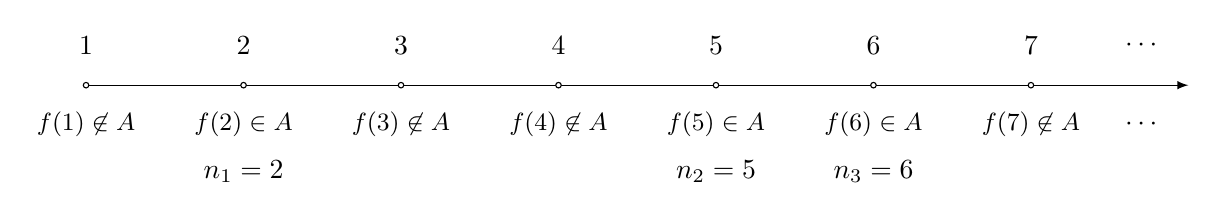
\begin{tikzpicture}
            \draw[-latex] (-7, 0) -- (7, 0);
            \foreach \i [evaluate=\i as \x using -9 + 2*\i] in {1,...,7}
            {
                \filldraw[draw=black, fill=white] (\x, 0) circle (1pt);
                \node at (\x, 0.5) {\i};
            }
            \node at (-7, -0.5) {\small \( f(1) \not\in A \)};

            \node at (-5, -0.5) {\small \( f(2) \in A \)};
            \node at (-5, -1.1) {\( n_1 = 2 \)};

            \node at (-3, -0.5) {\small \( f(3) \not\in A \)};

            \node at (-1, -0.5) {\small \( f(4) \not\in A \)};

            \node at (1, -0.5) {\small \( f(5) \in A \)};
            \node at (1, -1.1) {\( n_2 = 5 \)};

            \node at (3, -0.5) {\small \( f(6) \in A \)};
            \node at (3, -1.1) {\( n_3 = 6 \)};

            \node at (5, -0.5) {\small \( f(7) \not\in A \)};

            \node at (6.4, 0.5) {\( \cdots \)};
            \node at (6.4, -0.5) {\( \cdots \)};
        \end{tikzpicture}
        \caption{Example construction of \( (n_k)_{k=1}^{\infty} \)}
        \label{fig:ex1.5.1}
    \end{figure}

    \noindent It is clear from this construction that \( (n_k)_{k=1}^{\infty} \) is a strictly increasing sequence.
    
    Define \( g : \N \to A \) by \( g(k) = f(n_k) \); we claim that \( g \) is a bijection. For injectivity, observe that
    \[
        g(\ell) = g(k) \iff f(n_{\ell}) = f(n_k) \iff n_{\ell} = n_k \iff \ell = k,
    \]
    where we have used the injectivity of \( f \) for the second equivalence and the strict monotonicity of the sequence \( (n_k)_{k=1}^{\infty} \) for the third equivalence.

    For the surjectivity of \( g \), let \( a \in A \) be given. Since \( f \) is surjective, there is a positive integer \( N \) such that \( f(N) = a \); we need to find some \( k \in \N \) such that \( n_k = N \). It cannot be the case that \( N < n_1 \), otherwise \( n_1 \) would not be the minimum of \( \{ n \in \N : f(n) \in A \} \), so we must have \( n_1 \leq N \). Given this, and the fact that \( (n_k)_{k=1}^{\infty} \) is a strictly increasing sequence of natural numbers, there must exist a \( k \in \N \) such that \( n_k \leq N < n_{k + 1} \). In fact, it must be the case that \( n_k = N \), otherwise \( n_{k + 1 } \) would not be the minimum of \( \{ n \in \N : f(n) \in A \} \setminus \{ n_1, \ldots, n_k \} \). Thus \( g(k) = f(n_k) = f(N) = a \).
\end{solution}

\begin{exercise}
\label{ex:1.5.2}
    Review the proof of Theorem 1.5.6, part (ii) showing that \( \R \) is uncountable, and then find the flaw in the following erroneous proof that \( \Q \) is uncountable:

    Assume, for contradiction, that \( \Q \) is countable. Thus we can write \( \Q = \{ r_1, r_2, r_3, \ldots \} \) and, as before, construct a nested sequence of closed intervals with \( r_n \not\in I_n \). Our construction implies \( \bigcap_{n=1}^{\infty} I_n = \emptyset \) while NIP implies \( \bigcap_{n=1}^{\infty} I_n \neq \emptyset \). This contradiction implies \( \Q \) must therefore be uncountable.
\end{exercise}

\begin{solution}
    The construction does not imply that \( \bigcap_{n=1}^{\infty} I_n = \emptyset \); it only guarantees that this intersection does not contain any rational numbers.
\end{solution}

\begin{exercise}
\label{ex:1.5.3}
    Use the following outline to supply proofs for the statements in Theorem 1.5.8.
    \begin{enumerate}
        \item First, prove statement (i) for two countable sets, \( A_1 \) and \( A_2 \). Example 1.5.3 (ii) may be a useful reference. Some technicalities can be avoided by first replacing \( A_2 \) with the set \( B_2 = A_2 \setminus A_1 = \{ x \in A_2 : x \not\in A_1 \} \). The point of this is that the union \( A_1 \cup B_2 \) is equal to \( A_1 \cup A_2 \) and the sets \( A_1 \) and \( B_2 \) are disjoint. (What happens if \( B_2 \) is finite?)

        Now, explain how the more general statement in (i) follows.

        \item Explain why induction \textit{cannot} be used to prove part (ii) of Theorem 1.5.8 from part (i).

        \item Show how arranging \( \N \) into the two-dimensional array
        \[
            \begin{matrix}
            1 & 3 & 6 & 10 & 15 & \cdots \\
            2 & 5 & 9 & 14 & \cdots &  \\
            4 & 8 & 13 & \cdots &  &  \\
            7 & 12 & \cdots &   &  &  \\
            11 & \cdots &  &  &  &  \\
            \vdots &  &  &  &  & 
            \end{matrix}
        \]
        leads to a proof of Theorem 1.5.8 (ii).
    \end{enumerate}
\end{exercise}

\begin{solution}
    \begin{enumerate}
        \item As noted, it will suffice to show that \( A_1 \cup B_2 \) is countable, where \( B_2 = A_2 \setminus A_1 \). Since \( A_1 \) is countable, there exists a bijection \( f : \N \to A_1 \). Consider the following cases.
        \begin{description}
            \item[Case 1.] If \( B_2 \) is empty, then \( A_1 \cup B_2 = A_1 \), which is countable by assumption.

            \item[Case 2.] Suppose that \( B_2 \) is non-empty and finite, say \( B_2 = \{ x_1, \ldots, x_k \} \) for some \( k \in \N \). Define \( g : \N \to A_1 \cup B_2 \) by
            \[
                g(n) = \begin{cases}
                    x_n & \text{if } 1 \leq n \leq k, \\
                    f(n - k) & \text{if } k < n.
                \end{cases}
            \]
            \begin{figure}[h]
                \centering
                \begin{tikzpicture}
                    \node at (-4, 0) {\( \N \)};
                    \foreach \i [evaluate=\i as \x using -3.25 + 1.25 * \i] in {1,...,8}
                    {
                        \node at (\x, 0) {\i};
                    }
                    \node at (8, 0) {\( \cdots \)};

                    \node at (-4, -2) {\( A_1 \cup B_2 \)};
                    \foreach \i [evaluate=\i as \x using -3.25 + 1.25 * \i] in {1,...,3}
                    {
                        \node at (\x, -2) {\( x_{\i} \)};
                    }
                    \foreach \i [evaluate=\i as \x using 0.5 + 1.25 * \i] in {1,...,5}
                    {
                        \node at (\x, -2) {\( f(\i) \)};
                    }
                    \node at (8, -2) {\( \cdots \)};

                    \draw[->] (-4, -0.4) -- (-4, -1.6);
                    \foreach \i [evaluate=\i as \x using -3.25 + 1.25 * \i] in {1,...,8}
                    {
                        \draw[->] (\x, -0.4) -- (\x, -1.6);
                    }

                    \node at (-4.25, -1) {\( g \)};
                    \draw[line width=1.1pt, decorate, decoration={calligraphic brace, mirror, amplitude=5pt}] (-2.2, -2.4) -- (0.7, -2.4);
                    \node at (-0.75, -3) {\( B_2 \)};
                    \draw[line width=1.1pt, decorate, decoration={calligraphic brace, mirror, amplitude=5pt}] (1.35, -2.4) -- (7.15, -2.4);
                    \node at (4.25, -3) {\( A_1 \)};
                \end{tikzpicture}
                \caption{Example construction of \( g \) with \( B_2 = \{ x_1, x_2, x_3 \} \)}
                \label{fig:ex1.5.3}
            \end{figure}

            The injectivity of \( g \) follows as \( A_1 \) and \( B_2 \) are disjoint and \( f \) is injective. For the surjectivity of \( g \), it is clear that every element of \( B_2 \) belongs to the range of \( g \); the surjectivity of \( f \) implies that the elements of \( A_1 \) belong to the range of \( g \) also.

            \item[Case 3.] Suppose that \( B_2 \) is infinite. Since \( B_2 \) is a subset of the countable set \( A_2 \), \Cref{ex:1.5.1} implies that \( B_2 \) is countable, i.e., there exists a bijection \( h : \N \to B_2 \). Define \( g : \N \to A_1 \cup B_2 \) by
            \[
                g(n) = \begin{cases}
                    f \paren{ \tfrac{n}{2} } & \text{if } n \text{ is even}, \\
                    h \paren{ \tfrac{n+1}{2} } & \text{if } n \text{ is odd}.
                \end{cases}
            \]
            \vspace{4mm}
            \[
                \begin{tikzcd}[row sep = 12mm, column sep = 4mm]
                    \N \arrow[d, "g" {left, font=\normalsize}] & 1 \arrow[d] & 2 \arrow[d] & 3 \arrow[d] & 4 \arrow[d] & 5 \arrow[d] & \cdots \\
                    A_1 \cup B_2 & h(1) & f(1) & h(2) & f(2) & h(3) & \cdots
                \end{tikzcd}
            \]
            To see that \( g \) is injective, suppose that \( m \) and \( n \) are distinct positive integers.
            \begin{description}
                \item[Case 3.1] If both of \( m \) and \( n \) are even then \( g(m) \neq g(n) \) since \( f \) is injective.

                \item[Case 3.2] If both of \( m \) and \( n \) are odd then \( g(m) \neq g(n) \) since \( h \) is injective.

                \item[Case 3.3] If one of \( m \) and \( n \) is even and the other is odd then \( g(m) \neq g(n) \) since \( f \) maps into \( A_1 \), \( h \) maps into \( B_2 \), and \( A_1 \cap B_2 = \emptyset \).
            \end{description}
            To see that \( g \) is surjective, let \( x \in A_1 \cup B_2 \) be given. Since \( A_1 \cap B_2 = \emptyset \), exactly one of the statements \( x \in A_1 \) or \( x \in B_2 \) holds. Suppose \( x \in A_1 \). Because \( f \) is surjective, there is a positive integer \( n \) such that \( f(n) = x \); it follows that \( g(2n) = f(n) = x \). If \( x \in B_2 \), then the surjectivity of \( h \) implies that there is a positive integer \( n \) such that \( h(n) = x \); it follows that \( g(2n - 1) = h(n) = x \). We may conclude that \( g \) is a bijection and hence that \( A_1 \cup B_2 \) is countable.
        \end{description}

        A simple induction argument proves the more general statement in Theorem 1.5.8 (i). Let \( P(n) \) be the statement that for countable sets \( A_1, \ldots, A_n \), the union \( A_1 \cup \cdots \cup A_n \) is countable. The truth of \( P(1) \) is clear. Suppose that \( P(n) \) holds for some \( n \in \N \) and suppose we have countable sets \( A_1, \ldots, A_n, A_{n+1} \). Let \( A' = A_1 \cup \cdots \cup A_n \); the induction hypothesis guarantees that \( A' \) is countable. Observe that
        \[
            A_1 \cup \cdots \cup A_n \cup A_{n+1} = A' \cup A_{n+1}.
        \]
        Since \( A' \) and \( A_{n+1} \) are countable, the union \( A' \cup A_{n+1} \) is also countable by our previous proof, i.e., \( P(n+1) \) holds. This completes the induction step and the proof.

        \item Induction can only be used to show that a particular statement \( P(n) \) holds for each value of \( n \in \N \).

        \item For each \( n \in \N \) there exists a bijection \( f_n : \N \to A_n \). Let \( a_{mn} = f_n(m) \) and arrange these into another two-dimensional array like so:
        \[
            \begin{array}[b]{cccccc}
            A_1 & A_2 & A_3 & A_4 & A_5 & \cdots \\
            \hline
            a_{11} & a_{12} & a_{13} & a_{14} & a_{15} & \cdots \\
            a_{21} & a_{22} & a_{23} & a_{24} & \ddots \\
            a_{31} & a_{32} & a_{33} & \ddots \\
            a_{41} & a_{42} & \ddots \\
            a_{51} & \ddots \\
            \vdots
            \end{array}
            \qquad
            \begin{array}[b]{cccccc}
            1 & 3 & 6 & 10 & 15 & \cdots \\
            2 & 5 & 9 & 14 & \ddots \\
            4 & 8 & 13 & \ddots \\
            7 & 12 & \ddots \\
            11 & \ddots \\
            \vdots
            \end{array}
        \]
        Since each \( f_n \) is surjective, each element of \( \bigcup_{n=1}^{\infty} A_n \) appears somewhere in the left array. We define a function \( g : \bigcup_{n=1}^{\infty} A_n \to \N \) by working through the grid along the diagonals (first \( a_{11} \), then \( a_{21} \), then \( a_{12} \), then \( a_{31} \), and so on), mapping an element \( a_{mn} \) to the natural number appearing in the corresponding position in the right array. The \( A_n \)'s may have elements in common; if we encounter an element \( a_{mn} \) that we have already seen before, we simply skip this element and move on to the next one. In this way, we obtain an injective function \( g \). If we denote the range of \( g \) by \( B \subseteq \N \), then \( g : \bigcup_{n=1}^{\infty} A_n \to B \) is a bijection. Since the infinite set \( A_1 \) is contained in the union \( \bigcup_{n=1}^{\infty} A_n \) and \( g \) is injective, it must be the case that \( B \) is infinite; \Cref{ex:1.5.1} then implies that \( B \) is countable, i.e., there is a bijection \( h : \N \to B \). It follows that the function \( g^{-1} \circ h : \N \to \bigcup_{n=1}^{\infty} A_n \) is a bijection and we may conclude that \( \bigcup_{n=1}^{\infty} A_n \) is countable.
    \end{enumerate}
\end{solution}

\begin{exercise}
\label{ex:1.5.4}
    \begin{enumerate}
        \item Show \( (a, b) \sim \R \) for any interval \( (a, b) \).

        \item Show that an unbounded interval like \( (a, \infty) = \{ x : x > a \} \) has the same cardinality as \( \R \) as well.

        \item Using open intervals makes it more convenient to produce the required 1-1, onto functions, but it is not really necessary. Show that \( [0, 1) \sim (0, 1) \) by exhibiting a 1-1 onto function between the two sets.
    \end{enumerate}
\end{exercise}

\begin{solution}
    \begin{enumerate}
        \item Let \( f : (-1, 1) \to \R \) be the bijection given by \( f(x) = \tfrac{x}{x^2 - 1} \) (see Example 1.5.4 and \Cref{fig:ex1.5.4_1}) and let \( g : (a, b) \to (-1, 1) \) be given by \( g(x) = \tfrac{2(x - a)}{b - a} - 1 \) (see \Cref{fig:ex1.5.4_1}); it is straightforward to verify that \( g \) is a bijection. Thus \( (a, b) \sim (-1, 1) \sim \R \) and it follows that \( (a, b) \sim \R \) (\Cref{ex:1.5.5}).

        \begin{figure}[t]
            \centering
            \begin{subfigure}{0.42\textwidth}
                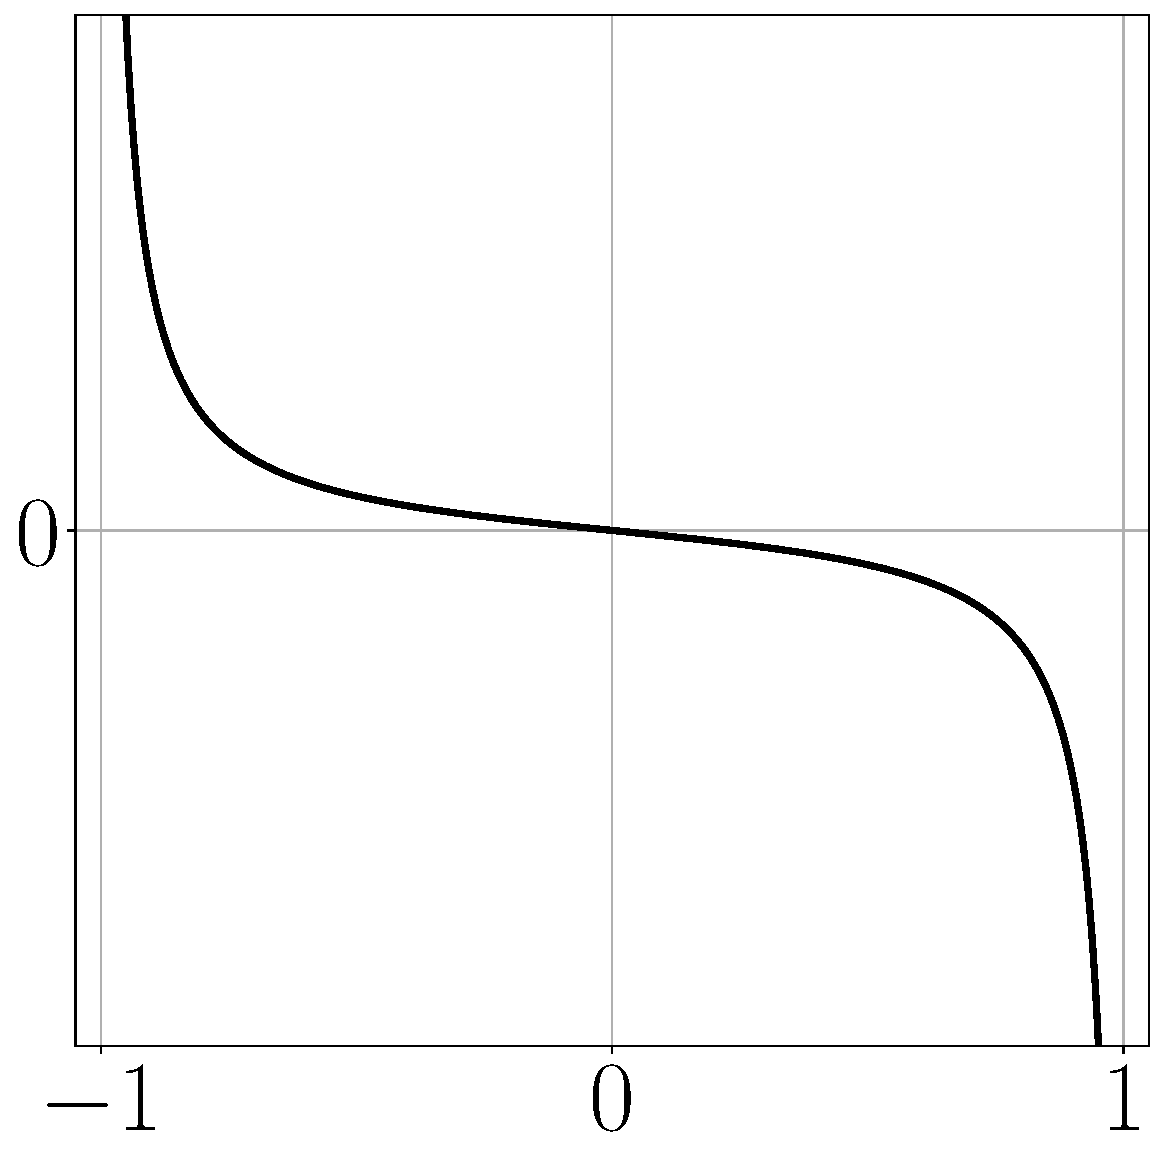
\includegraphics[width=\textwidth]{UA_Figures/UA_ex1_5_4_fig_1_a.pdf}
                \caption{\( f(x) = \tfrac{x}{x^2 - 1} \) on \( (-1, 1) \)}
            \end{subfigure}
            \begin{subfigure}{0.42\textwidth}
                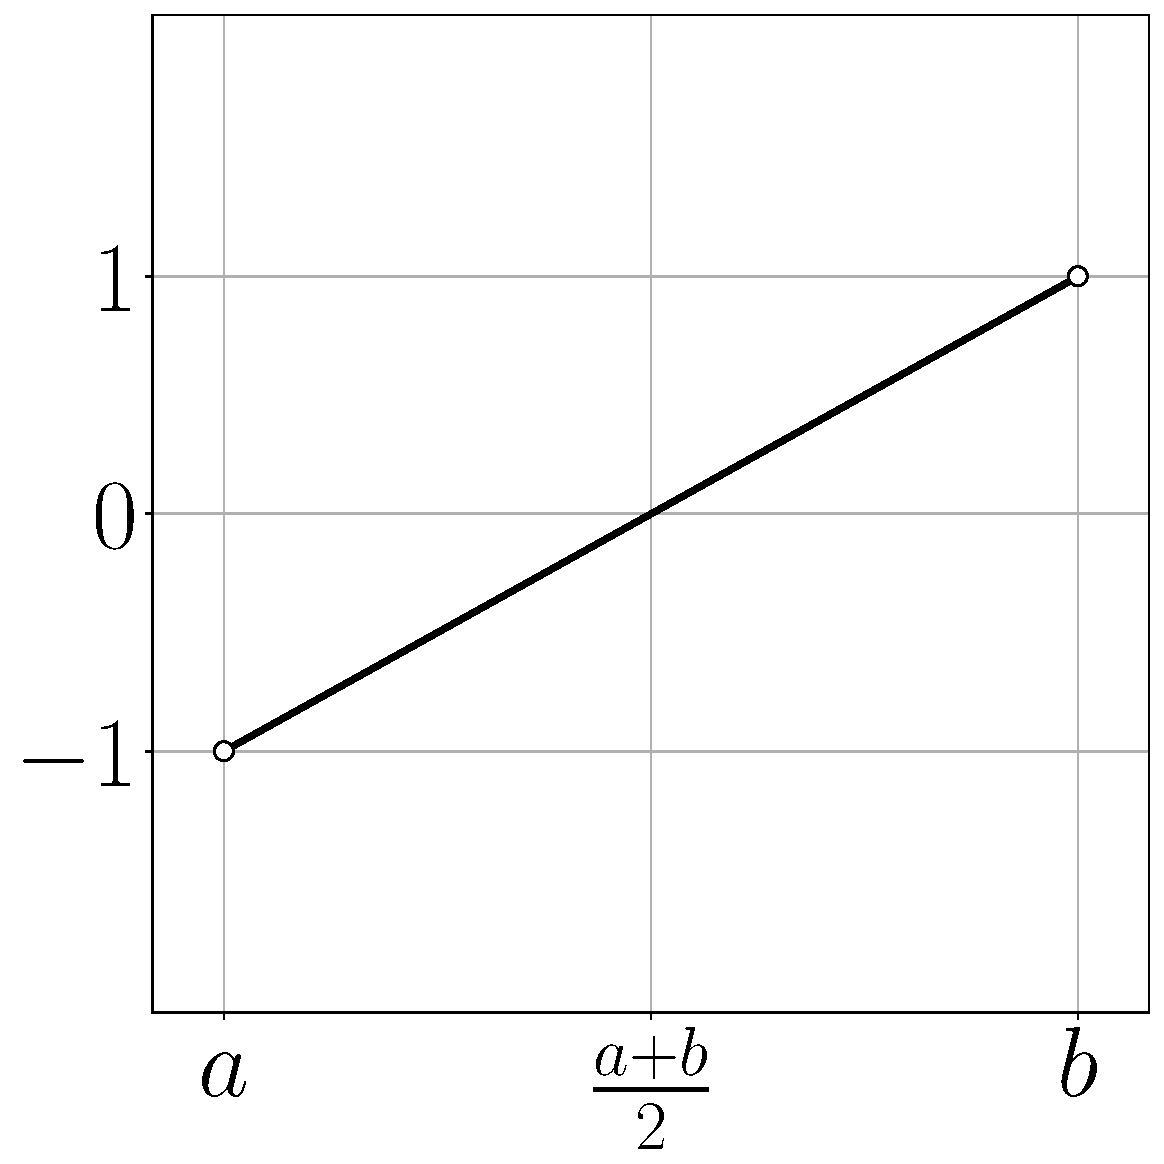
\includegraphics[width=\textwidth]{UA_Figures/UA_ex1_5_4_fig_1_b.pdf}
                \caption{\( g(x) = \tfrac{2(x - a)}{b - a} - 1 \) on \( (a, b) \)}
            \end{subfigure}
            \caption{Bijections \( f : (-1, 1) \to \R \) and \( g : (a, b) \to (-1, 1) \)}
            \label{fig:ex1.5.4_1}
        \end{figure}

        \item Let \( f : (a, \infty) \to (0, 1) \) be the bijection given by \( f(x) = \tfrac{1}{x + 1 - a} \) (see \Cref{fig:ex1.5.4_2}). Thus \( (a, \infty) \sim (0, 1) \) and, by part (a), \( (0, 1) \sim \R \); it follows from \Cref{ex:1.5.5} that \( (a, \infty) \sim \R \).

        \begin{figure}[H]
            \centering
            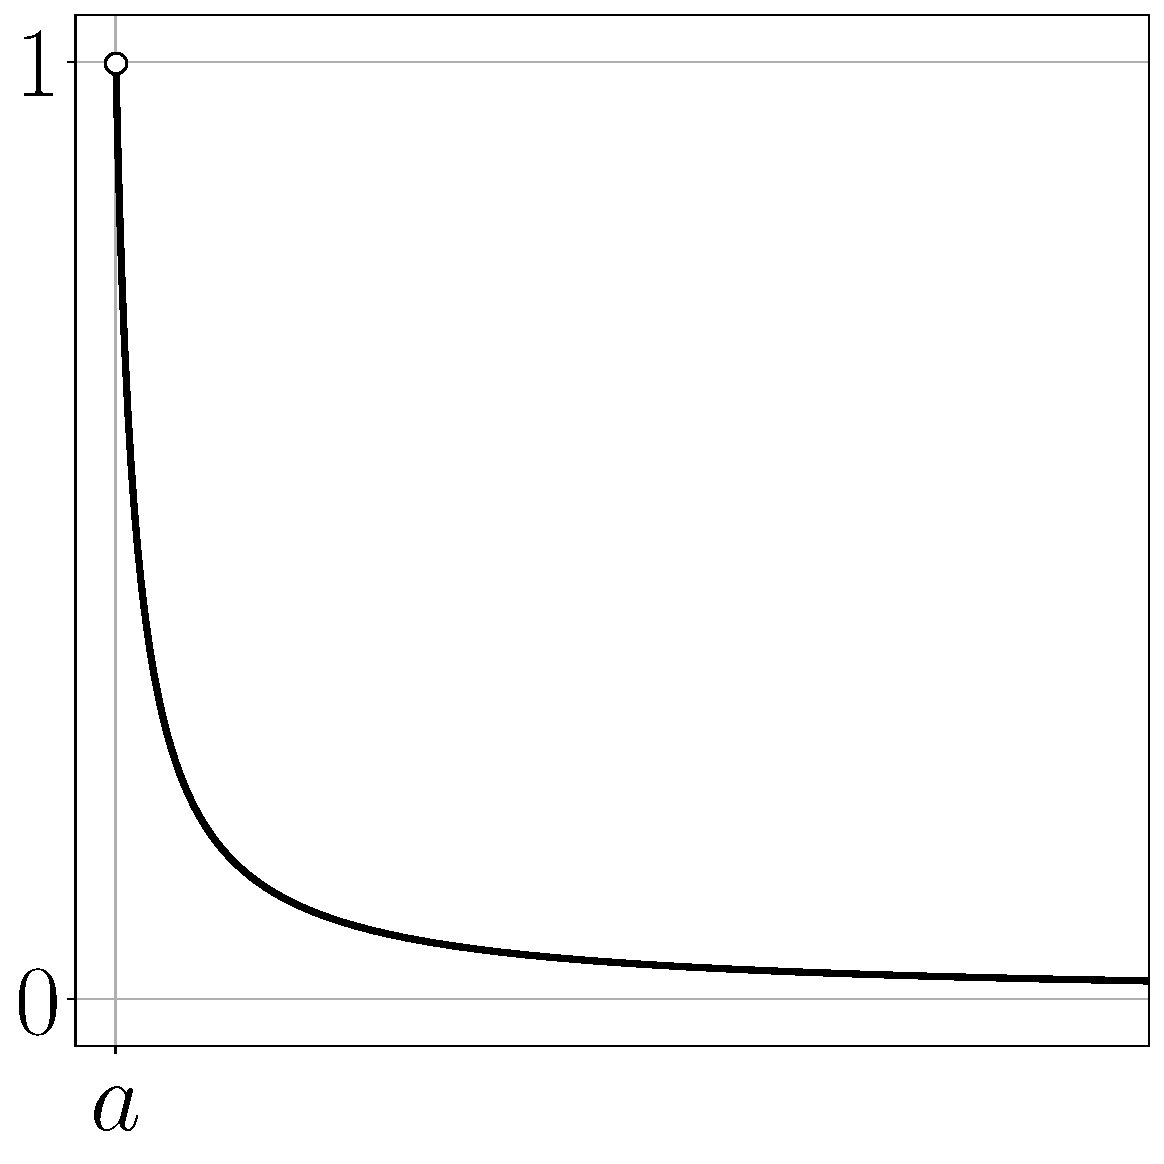
\includegraphics[width=0.42\textwidth]{UA_Figures/UA_ex1_5_4_fig_2.pdf}
            \caption{Bijection \( f : (a, \infty) \to (0, 1) \) given by \( f(x) = \tfrac{1}{x + 1 - a} \)}
            \label{fig:ex1.5.4_2}
        \end{figure}

        \item It is clear that \( [0, 1) \sim (0, 1] \) via the map \( x \mapsto 1 - x \) and so, by \Cref{ex:1.5.5}, it will suffice to show that \( (0, 1) \sim (0, 1] \). Define a function \( f : (0, 1) \to (0, 1] \) by
        \[
            f(x) = \begin{cases}
                \tfrac{1}{n} & \text{if } x = \tfrac{1}{n + 1} \text{ for some } n \in \N, \\
                x & \text{otherwise}.
            \end{cases}
        \]
        This function is a bijection since it has an inverse \( f^{-1} : (0, 1] \to (0, 1) \) given by
        \[
            f^{-1}(x) = \begin{cases}
                \tfrac{1}{n + 1} & \text{if } x = \tfrac{1}{n} \text{ for some } n \in \N, \\
                x & \text{otherwise}.
            \end{cases}
        \]
        See \Cref{fig:ex1.5.4_3} for a graph of \( f \) and \( f^{-1} \).

        \begin{figure}[H]
            \centering
            \begin{subfigure}{0.49\textwidth}
                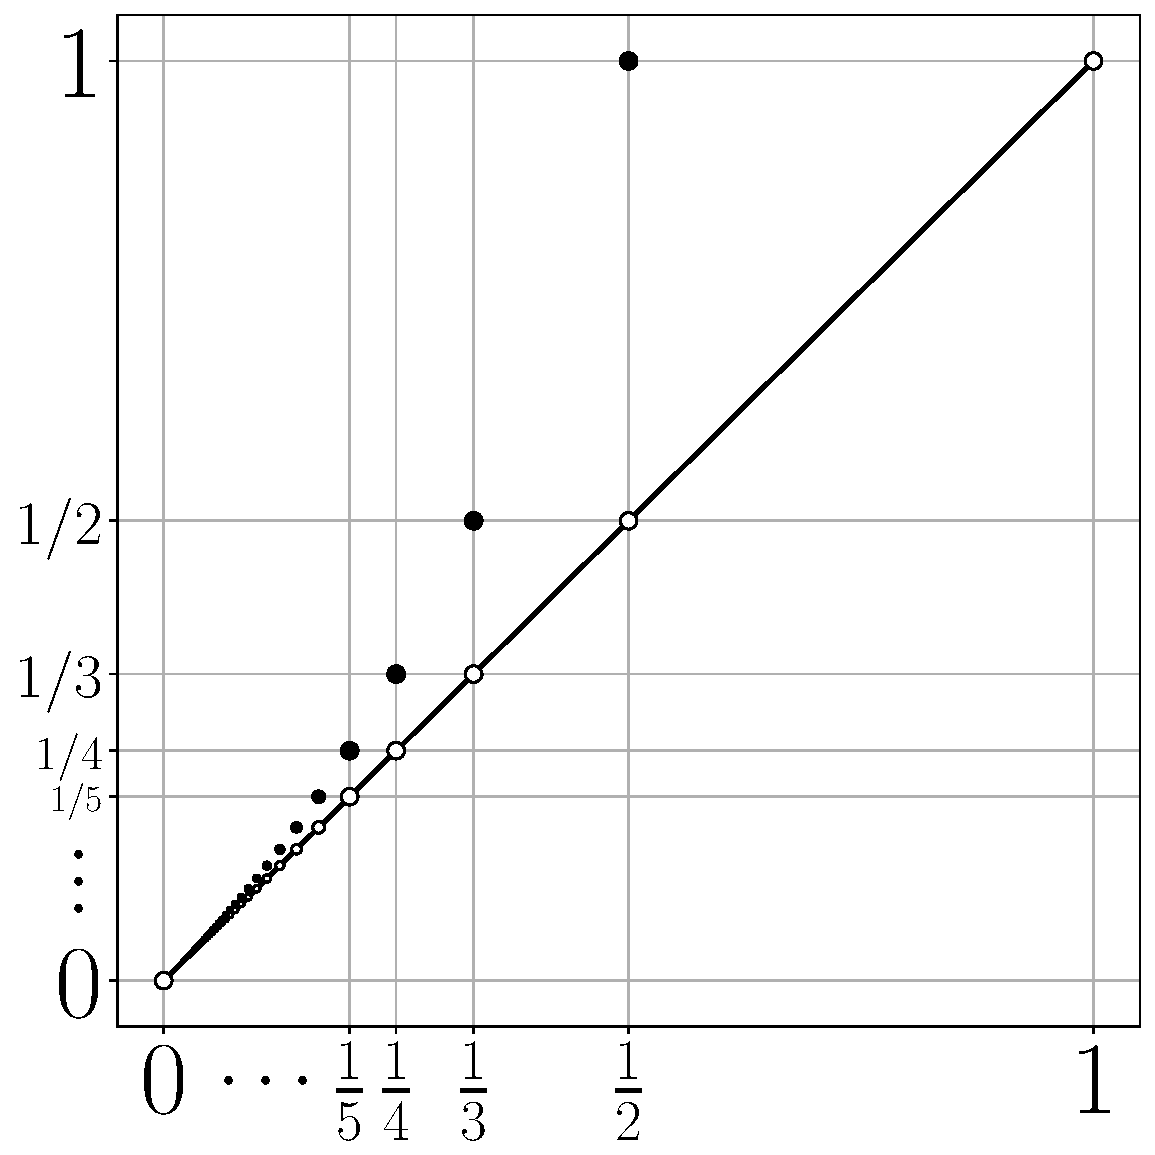
\includegraphics[width=\textwidth]{UA_Figures/UA_ex1_5_4_fig_3_a.pdf}
                \caption{\( f \) on \( (0, 1) \)}
            \end{subfigure}
            \begin{subfigure}{0.49\textwidth}
                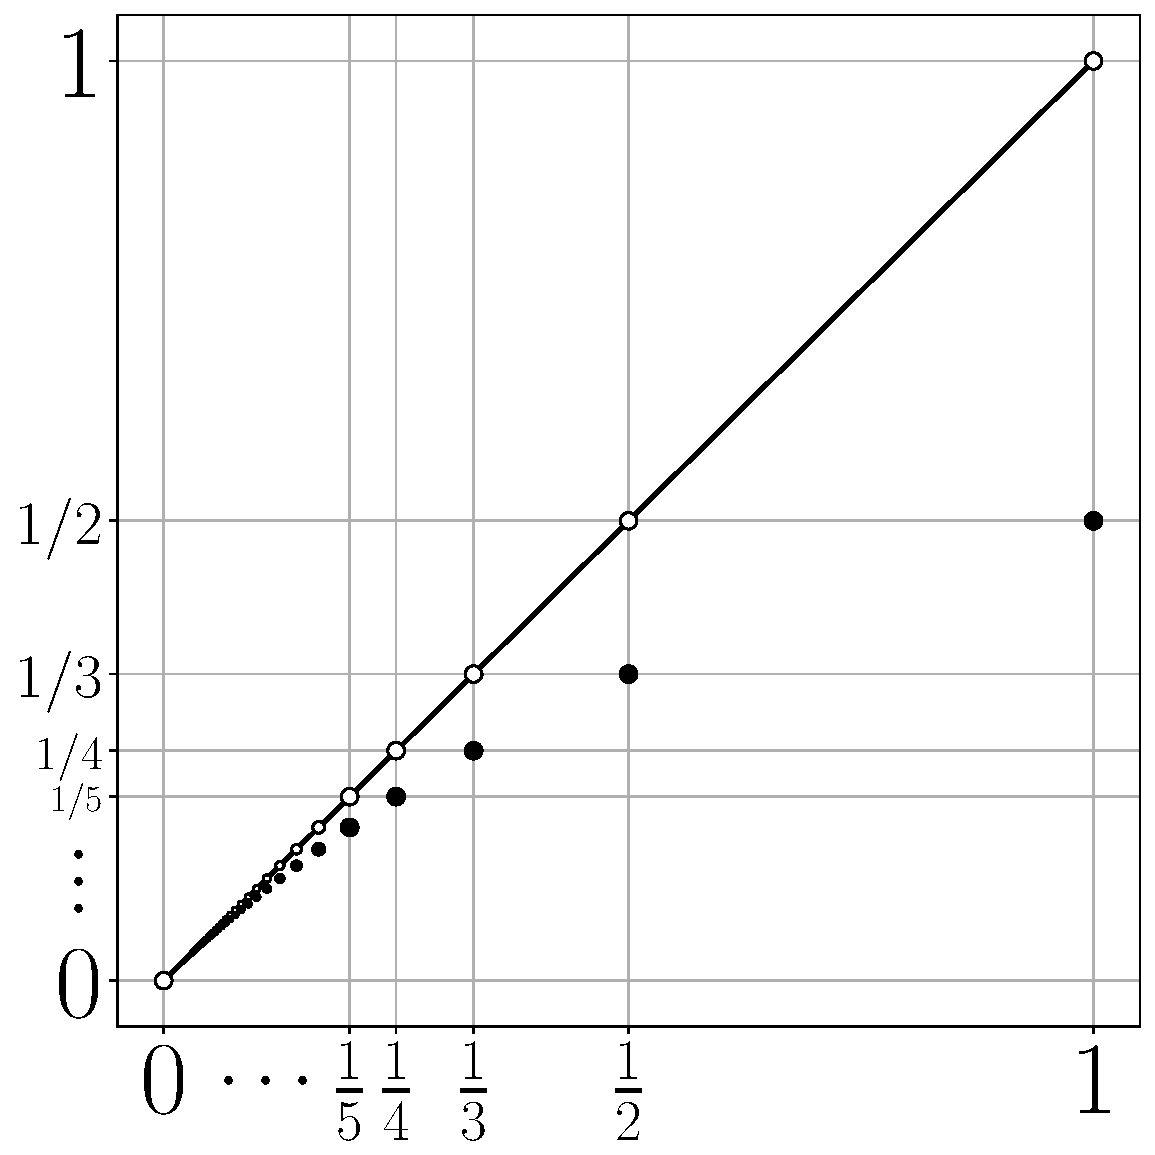
\includegraphics[width=\textwidth]{UA_Figures/UA_ex1_5_4_fig_3_b.pdf}
                \caption{\( f^{-1} \) on \( (0, 1] \)}
            \end{subfigure}
            \caption{Bijections \( f : (0, 1) \to (0, 1] \) and \( f^{-1} : (0, 1] \to (0, 1) \)}
            \label{fig:ex1.5.4_3}
        \end{figure}
    \end{enumerate}
\end{solution}

\begin{exercise}
\label{ex:1.5.5}
    \begin{enumerate}
        \item Why is \( A \sim A \) for every set \( A \)?

        \item Given sets \( A \) and \( B \), explain why \( A \sim B \) is equivalent to asserting \( B \sim A \).

        \item For three sets \( A, B, \) and \( C \), show that \( A \sim B \) and \( B \sim C \) implies \( A \sim C \). These three properties are what is meant by saying that \( \sim \) is an \textit{equivalence relation}.
    \end{enumerate}
\end{exercise}

\begin{solution}
    \begin{enumerate}
        \item The identity function \( f : A \to A \) given by \( f(x) = x \) is a bijection.

        \item Since \( A \sim B \), there is a bijection \( f : A \to B \). A function is bijective if and only if it has an inverse function \( f^{-1} : B \to A \), which must also be bijective.

        \item There are bijections \( f : A \to B \) and \( g : B \to C \). It follows that the composition \( g \circ f : A \to C \) is also a bijection.
    \end{enumerate}
\end{solution}

\begin{exercise}
\label{ex:1.5.6}
    \begin{enumerate}
        \item Give an example of a countable collection of disjoint open intervals.

        \item Give an example of an uncountable collection of disjoint open intervals, or argue that no such collection exists.
    \end{enumerate}
\end{exercise}

\begin{solution}
    \begin{enumerate}
        \item Take \( A_n = (n, n+1) \) for \( n \in \N \).

        \item No such collection exists. To see this, suppose there was such a collection \( \{ I_a : a \in A \} \) for some uncountable set \( A \). By the density of \( \Q \) in \( \R \), there exists a rational number \( r_a \in I_a \) for each \( a \in A \). Since the intervals are disjoint, each \( r_a \) must be distinct and hence the collection \( \{ r_a : a \in A \} \) must be an uncountable subset of \( \Q \)---but this contradicts \Cref{ex:1.5.1}.
    \end{enumerate}
\end{solution}

\begin{exercise}
\label{ex:1.5.7}
    Consider the open interval \( (0, 1) \), and let \( S \) be the set of points in the open unit square; that is, \( S = \{ (x, y) : 0 < x, y < 1 \} \).
    \begin{enumerate}
        \item Find a 1-1 function that maps \( (0, 1) \) into, but not necessarily onto, \( S \). (This is easy.)

        \item Use the fact that every real number has a decimal expansion to produce a 1-1 function that maps \( S \) into \( (0, 1) \). Discuss whether the formulated function is onto. (Keep in mind that any terminating decimal expansion such as \( .235 \) represents the same real number as \( .234999 \ldots \) .)
    \end{enumerate}
    The Schröder-Bernstein Theorem discussed in \Cref{ex:1.5.11} can now be applied to conclude that \( (0, 1) \sim S \).
\end{exercise}

\begin{solution}
    \begin{enumerate}
        \item Take \( f : (0, 1) \to S \) given by \( f(x) = \paren{x, \tfrac{1}{2}} \).

        \item For \( (x, y) \in S \), suppose \( x \) has decimal representation \( 0.x_1 x_2 x_3 \ldots \) and \( y \) has decimal representation \( 0.y_1 y_2 y_3 \ldots  \), where if necessary we choose the decimal representation terminating in 0's. To define \( g : S \to (0, 1) \), let \( g(x, y) = 0.x_1 y_1 x_2 y_2 x_3 y_3 \ldots \)
        
        For the injectivity of \( g \), suppose we have \( (x, y) \neq (a, b) \) in \( S \), so that at least one of \( x \neq a \) or \( y \neq b \) holds. Assuming \( x \neq a \) (the case where \( y \neq b \) is handled similarly), let \( 0.x_1 x_2 x_3 \ldots \) be the decimal representation of \( x \) and let \( 0.a_1 a_2 a_3 \ldots \) be the decimal representation of \( a \). Since \( x \neq a \), there must be some index \( n \) such that \( x_n \neq a_n \). If \( g(x, y) \) has decimal representation \( 0.s_1 s_2 s_3 \ldots \) and \( g(a, b) \) has decimal representation \( 0.t_1 t_2 t_3 \ldots \), then
        \[
            s_{2n - 1} = x_n \neq a_n = t_{2n - 1}.
        \]
        This implies that \( g(x, y) \neq g(a, b) \), provided it is not the case that \( g(x, y) \) terminates in 0's and \( g(a, b) \) terminates in 9's, or vice versa. To rule this out, note that \( g(a, b) \) terminates in 9's only if both \( a \) and \( b \) terminate in 9's---but our construction specifically chooses the decimal representations for \( a \) and \( b \) terminating in 0's if necessary. The case where \( g(x, y) \) terminates in 9's is handled similarly.

        This function \( g \) is not surjective since \( 0.1 \) does not belong to the range of \( g \). Indeed,
        \[
            g(x, y) = 0.x_1 y_1 x_2 y_2 \ldots = 0.1000 \ldots
        \]
        implies that \( y = 0 \), but \( (x, 0) \not\in S \) for any \( x \in (0, 1) \).
    \end{enumerate}
\end{solution}

\begin{exercise}
\label{ex:1.5.8}
    Let \( B \) be a set of positive real numbers with the property that adding together any finite subset of elements from \( B \) always gives a sum of 2 or less. Show \( B \) must be finite or countable.
\end{exercise}

\begin{solution}
    Suppose \( a \in (0, 1] \); we claim that \( B \cap (a, 2] \) must be a (possibly empty) finite set. By the Archimedean Property (Theorem 1.4.2), there is an \( n \in \N \) such that \( na > 2 \). If \( B \cap (a, 2] \) contains at least \( n \) elements, say \( \{ b_1, \ldots, b_n \} \), then since each \( b_i > a \) we have
    \[
        b_1 + \cdots + b_n > na > 2.
    \]
    This contradicts our hypotheses, so it must be the case that \( B \cap (a, 2] \) contains less than \( n \) elements and our claim follows.

    Any element of \( B \) must be less than or equal to 2, so \( B \subseteq (0, 2] \) and it follows that
    \[
        B = \bigcup_{n=1}^{\infty} \paren{ B \cap \left( \tfrac{1}{n}, 2 \right] }.
    \]
    This expresses \( B \) as a countable union of finite sets and thus \( B \) is either finite or countable (Theorem 1.5.8).
\end{solution}

\begin{exercise}
\label{ex:1.5.9}
    A real number \( x \in \R \) is called \textit{algebraic} if there exist integers \( a_0, a_1, \) \( a_2, \ldots, a_n \in \Z \), not all zero, such that
    \[
        a_n x^n + a_{n-1} x^{n-1} + \cdots + a_1 x + a_0 = 0.
    \]
    Said another way, a real number is algebraic if it is the root of a polynomial with integer coefficients. Real numbers that are not algebraic are called \textit{transcendental} numbers. Reread the last paragraph of Section 1.1. The final question posed here is closely related to the question of whether or not transcendental numbers exist.
    \begin{enumerate}
        \item Show that \( \sqrt{2}, \sqrt[3]{2} \), and \( \sqrt{3} + \sqrt{2} \) are algebraic.

        \item Fix \( n \in \N \), and let \( A_n \) be the algebraic numbers obtained as roots of polynomials with integer coefficients that have degree \( n \). Using the fact that every polynomial has a finite number of roots, show that \( A_n \) is countable.

        \item Now, argue that the set of all algebraic numbers is countable. What may we conclude about the set of transcendental numbers?
    \end{enumerate}
\end{exercise}

\begin{solution}
    \begin{enumerate}
        \item \( \sqrt{2} \) is a root of the polynomial \( x^2 - 2 \), \( \sqrt[3]{2} \) is a root of the polynomial \( x^3 - 2 \), and \( \sqrt{3} + \sqrt{2} \) is a root of the polynomial \( x^4 - 10 x^2 + 1 \).

        \item We will use the following useful corollary of Theorem 1.5.8 (ii).
        \begin{lemma}
        \label{lem:ex1.5.9}
            If \( A_1, \ldots, A_n \) are countable sets, then \( A_1 \times \cdots \times A_n \) is also countable.
        \end{lemma}

        \begin{proof}
            Suppose that \( A \) and \( B \) are countable sets, so that \( B = \{ b_1, b_2, b_3, \ldots \} \). For each \( n \in \N \), it is clear that the set \( A \times \{ b_n \} \) is countable. Now observe that
            \[
                A \times B = \bigcup_{n=1}^{\infty} \paren{ A \times \{ b_n \} }.
            \]
            It follows from Theorem 1.5.8 (ii) that \( A \times B \) is countable. A straightforward induction argument proves the general case.
        \end{proof}
        
        Let \( P_n \) be the collection of polynomials with integer coefficients that have degree \( n \), i.e.\ \( P_n = \{ a_n x^n + a_{n-1} x^{n-1} + \cdots + a_1 x + a_0 : a_n, \ldots, a_0 \in \Z, a_n \neq 0 \} \). Notice that
        \[
            P_n \sim (\Z \setminus \{ 0 \}) \times \underbrace{\Z \times \cdots \times \Z}_{n \text{ times}}
        \]
        via the map
        \[
            a_n x^n + a_{n-1} x^{n-1} + \cdots + a_1 x + a_0 \mapsto (a_n, a_{n-1}, \ldots, a_1, a_0).
        \]
        It then follows from \Cref{lem:ex1.5.9} that \( P_n \) is countable. For a polynomial \( p \in P_n \), let \( R_p \) be the set of its roots, i.e., \( R_p = \{ x \in \R : p(x) = 0 \} \), and note that \( R_p \) is always a finite set. Now observe that
        \[
            A_n = \bigcup_{p \in P_n} R_p,
        \]
        demonstrating that \( A_n \) is a countable union of finite sets; it follows from Theorem 1.5.8 that \( A_n \) is either finite or countable. Since \( \sqrt[n]{k} \in A_n \) for each \( k \in \N \) (it is a root of the polynomial \( x^n - k \)), we see that \( A_n \) must be infinite and hence countable.

        \item If we let \( A \) be the set of all algebraic numbers then \( A = \bigcup_{n=1}^{\infty} A_n \), i.e., \( A \) is a countable union of countable sets. It follows from Theorem 1.5.8 (ii) that \( A \) is countable.

        A consequence of this is that the set of transcendental numbers \( \setcomp{A} \) must be uncountable. To see this, note that \( \R = A \cup \setcomp{A} \), the union of two countable sets is countable, and \( \R \) is not countable.
    \end{enumerate}
\end{solution}

\begin{exercise}
\label{ex:1.5.10}
    \begin{enumerate}
        \item Let \( C \subseteq [0, 1] \) be uncountable. Show that there exists \( a \in (0, 1) \) such that \( C \cap [a, 1] \) is uncountable.

        \item Now let \( A \) be the set of all \( a \in (0, 1) \) such that \( C \cap [a, 1] \) is uncountable, and let \( \alpha = \sup A \). Is \( C \cap [\alpha, 1] \) an uncountable set?

        \item Does the statement in (a) remain true if ``uncountable" is replaced by ``infinite"?
    \end{enumerate}
\end{exercise}

\begin{solution}
    \begin{enumerate}
        \item If we suppose that for each \( a \in (0, 1) \) the set \( C \cap [a, 1] \) is countable, then we can express \( C \) as a countable union of countable sets:
        \[
            C = \bigcup_{n=2}^{\infty} \paren{ C \cap \bkt{ \frac{1}{n}, 1 } }.
        \]
        This implies that \( C \) is countable (Theorem 1.5.8 (ii)). Thus, given that \( C \) is uncountable, there must exist some \( a \in (0, 1) \) such that \( C \cap [a, 1] \) is uncountable. 

        \item Not necessarily. Suppose \( C = [0, 1] \). Then for all \( a \in (0, 1) \), we have \( C \cap [a, 1] = [a, 1] \), which is uncountable. Thus \( A = (0, 1) \) and it follows that \( \alpha = \sup A = 1 \), but \( C \cap [\alpha, 1] = \{ 1 \} \) is not uncountable.

        \item The statement is no longer true in general. If we let \( C = \set{ \tfrac{1}{n} : n \in \N } \) then no matter which \( a \in (0, 1) \) we choose, the intersection \( C \cap [a, 1] \) is a finite set (since there are only finitely many positive integers less than or equal to \( a^{-1} \), there are only finitely many reciprocals of positive integers greater than or equal to \( a \)).
    \end{enumerate}
\end{solution}

\begin{exercise}[Schröder-Bernstein Theorem]
\label{ex:1.5.11}
    Assume there exists a 1-1 function \( f : X \to Y \) and another 1-1 function \( g : Y \to X \). Follow the steps to show that there exists a 1-1, onto function \( h : X \to Y \) and hence \( X \sim Y \).

    The strategy is to partition \( X \) and \( Y \) into components
    \[
        X = A \cup A' \quad \text{and} \quad Y = B \cup B'
    \]
    with \( A \cap A' = \emptyset \) and \( B \cap B' = \emptyset \), in such a way that \( f \) maps \( A \) onto \( B \), and \( g \) maps \( B' \) onto \( A' \).
    \begin{enumerate}
        \item Explain how achieving this would lead to a proof that \( X \sim Y \).

        \item Set \( A_1 = X \setminus g(Y) = \{ x \in X : x \not\in g(Y) \} \) (what happens if \( A_1 = \emptyset \)?) and inductively define a sequence of sets by letting \( A_{n+1} = g(f(A_n)) \). Show that \( \{ A_n : n \in \N \} \) is a pairwise disjoint collection of subsets of \( X \), while \( \{ f(A_n) : n \in \N \} \) is a similar collection in \( Y \).

        \item Let \( A = \bigcup_{n=1}^{\infty} A_n \) and \( B = \bigcup_{n=1}^{\infty} f(A_n) \). Show that \( f \) maps \( A \) onto \( B \).

        \item Let \( A' = X \setminus A \) and \( B' = Y \setminus B \). Show \( g \) maps \( B' \) onto \( A' \).
    \end{enumerate}
\end{exercise}

\begin{solution}
    \begin{enumerate}
        \item Abusing notation slightly, we have bijections \( f : A \to B \) and \( g : B' \to A' \), and their inverses \( f^{-1} : B \to A \) and \( g^{-1} : A' \to B' \). Since \( A \cap A' = \emptyset \) and \( B \cap B' = \emptyset \), the functions \( h : X \to Y \) and \( h' : Y \to X \) given by
        \[
            h(x) = \begin{cases}
                f(x) & \text{if } x \in A, \\
                g^{-1}(x) & \text{if } x \in A',
            \end{cases}
            \qquad
            h'(y) = \begin{cases}
                f^{-1}(y) & \text{if } y \in B, \\
                g(y) & \text{if } y \in B'
            \end{cases}
        \]
        are well-defined. It is straightforward to verify that \( h \) and \( h' \) are mutual inverses and thus \( X \sim Y \).

        \item If \( A_1 \) is empty then \( X = g(Y) \), i.e., \( g \) is surjective. Since \( g \) is injective by assumption, it immediately follows that \( X \sim Y \) via \( g \).

        Let \( P(n) \) be the statement that \( \{ A_1, \ldots, A_n \} \) is a pairwise disjoint collection of sets; to prove that \( \{ A_n : n \in \N \} \) is a pairwise disjoint collection, we will first use induction to prove that \( P(n) \) holds for all \( n \in \N \). The truth of \( P(1) \) is clear, so suppose that \( P(n) \) holds for some \( n \in \N \). To demonstrate the truth of \( P(n+1) \), we need to show that \( A_k \cap A_{n+1} = \emptyset \) for all \( 1 \leq k \leq n \). Because \( A_{n+1} = g(f(A_n)) \subseteq g(Y) \) and \( A_1 = X \setminus g(Y) \), we see that \( A_1 \cap A_{n+1} = \emptyset \). If \( n \geq 2 \), suppose that \( 2 \leq k \leq n \) and observe that
        \begin{align*}
            A_k \cap A_{n+1} &= g(f(A_{k-1})) \cap g(f(A_n)) \\
            &= g(f(A_{k-1} \cap A_n)) \tag{\( f \) and \( g \) are injective} \\
            &= g(f(\emptyset)) \tag{induction hypothesis} \\
            &= \emptyset.
        \end{align*}
        Hence \( P(n+1) \) holds; this completes the induction step and it follows that \( P(n) \) holds for all \( n \in \N \).
        
        We can now show that \( \{ A_n : n \in \N \} \) is a pairwise disjoint collection of sets. Let \( A_m \) and \( A_n \) be given and suppose without loss of generality that \( m < n \). By the previous paragraph the collection \( \{ A_1, \ldots, A_m, \ldots A_n \} \) is pairwise disjoint and thus \( A_m \cap A_n = \emptyset \).
        
        That \( \{ f(A_n) : n \in \N \} \) is a pairwise disjoint collection now follows immediately from the injectivity of \( f \).

        \item Observe that
        \[
            f(A) = f \paren{ \bigcup_{n=1}^{\infty} A_n } = \bigcup_{n=1}^{\infty} f(A_n) = B,
        \]
        where we have used that the image of a union is the union of the images; the proof of this is similar to the proof of the special case given in \Cref{ex:1.2.7} (d).

        \item Notice that
        \begin{align*}
            b \in B' & \iff b \not\in f(A_n) \text{ for all } n \in \N \\[2mm]
            & \iff g(b) \not\in g(f(A_n)) \text{ for all } n \in \N \tag{\( g \) is injective} \\[2mm]
            & \iff g(b) \not\in A_{n+1} \text{ for all } n \in \N \\[2mm]
            & \iff g(b) \not\in A_n \text{ for all } n \geq 2.
        \end{align*}
        Notice further that \( g(y) \not\in X \setminus g(Y) = A_1 \) for any \( y \in Y \). It follows that
        \[
            b \in B' \iff g(b) \not\in A_n \text{ for all } n \in \N \iff g(b) \in A'. \tag{\( * \)}
        \]
        Thus \( g \) maps \( B' \) into \( A' \). To see that \( g : B' \to A' \) is surjective, observe that for any \( a \in A' \) we have, in particular, \( a \not\in A_1 = X \setminus g(Y) \), so that \( a \in g(Y) \), i.e., \( a = g(y) \) for some \( y \in Y \). It then follows from \( (*) \) that \( y \in B' \).
    \end{enumerate}
\end{solution}

\section{Cantor's Theorem}
\label{sec:1.6}

\begin{exercise}
\label{ex:1.6.1}
    Show that \( (0, 1) \) is uncountable if and only if \( \R \) is uncountable. This shows that Theorem 1.6.1 is equivalent to Theorem 1.5.6.
\end{exercise}

\begin{solution}
    We have \( (0, 1) \sim \R \) by \Cref{ex:1.5.4} (a).
\end{solution}

\begin{exercise}
\label{ex:1.6.2}
    \begin{enumerate}
        \item Explain why the real number \( x = .b_1 b_2 b_3 b_4 \ldots \) cannot be \( f(1) \).

        \item Now, explain why \( x \neq f(2) \), and in general why \( x \neq f(n) \) for any \( n \in \N \).

        \item Point out the contradiction that arises from these observations and conclude that \( (0, 1) \) is uncountable.
    \end{enumerate}
\end{exercise}

\begin{solution}
    \begin{enumerate}
        \item We have decimal expansions
        \[
            f(1) = .a_{11} a_{12} a_{13} a_{14} \ldots \hspaceand x = .b_1 b_2 b_3 b_4 \ldots.
        \]
        By construction, \( b_1 \neq a_{11} \). This implies that \( f(1) \neq x \), provided these decimal expansions are not two different representations of the same real number (for example, .3 and \( .2999 \ldots \)). However, since the only way this can occur is when one decimal expansion terminates in repeating 0's and the other terminates in repeating 9's, and the digits \( b_n \) are always either 2 or 3, we see that \( .b_1 b_2 b_3 b_4 \ldots \) must be the unique decimal representation of a real number.

        \item Since \( .b_1 b_2 b_3 b_4 \ldots \) is the unique decimal expansion of the real number \( x \) (see part (a)) and \( b_n \neq a_{nn} \), we have \( x \neq f(n) \) for every \( n \in \N \). Here is an example construction of \( x \) given some function \( f : \N \to (0, 1) \):
        \[
            \begin{matrix}
                f(1) & = & 0 & . & \textcolor{red}{9} & 2 & 8 & 4 & 7 & 6 & \ldots \\[1mm]
                f(2) & = & 0 & . & 2 & \textcolor{red}{2} & 8 & 4 & 9 & 1 & \ldots \\[1mm]
                f(3) & = & 0 & . & 9 & 9 & \textcolor{red}{1} & 0 & 2 & 5 & \ldots \\[1mm]
                f(4) & = & 0 & . & 2 & 1 & 1 & \textcolor{red}{9} & 2 & 1 & \ldots \\[1mm]
                f(5) & = & 0 & . & 1 & 2 & 5 & 7 & \textcolor{red}{2} & 3 & \ldots \\[1mm]
                f(6) & = & 0 & . & 9 & 7 & 7 & 5 & 1 & \textcolor{red}{8} & \ldots \\[1mm]
                \vdots & & & & & & & & & & \\[1mm]
                x & = & 0 & . & 2 & 3 & 2 & 2 & 3 & 2 & \ldots
            \end{matrix}
        \]
        Notice how the first digit (after the decimal point) of \( x \) differs from the first digit of \( f(1) \), the second digit of \( x \) differs from the second digit of \( f(2) \), and so on.

        \item The real number \( x \) belongs to \( (0, 1) \) but not to the image of \( f \), which contradicts our assumption that \( f \) was surjective. It follows that there cannot exist a bijection between \( \N \) and \( (0, 1) \). Since \( (0, 1) \) is clearly infinite, we may conclude that \( (0,1 ) \) is uncountable.
    \end{enumerate}
\end{solution}

\begin{exercise}
\label{ex:1.6.3}
    Supply rebuttals to the following complaints about the proof of Theorem 1.6.1.
    \begin{enumerate}
        \item Every rational number has a decimal expansion, so we could apply this same argument to show that the set of rational numbers between 0 and 1 is uncountable. However, because we know that any subset of \( \Q \) must be countable, the proof of Theorem 1.6.1 must be flawed.

        \item Some numbers have \textit{two} different decimal representations. Specifically, any decimal expansion that terminates can also be written with repeating 9's. For instance, \( 1/2 \) can also be written as \( .5 \) or as \( .4999 \ldots \, \). Doesn't this cause some problems?
    \end{enumerate}
\end{exercise}

\begin{solution}
    \begin{enumerate}
        \item The problem with this reasoning is that the real number
        \[
            x = .b_1 b_2 b_3 b_4 \ldots
        \]
        that we construct may not be rational. For example, consider the function \( f : \N \to (0, 1) \cap \Q \) given by
        \[
        \begin{aligned}
            f(1) &= .3, \\
            f(2) &= .02, \\
            f(3) &= .003, \\
            f(4) &= .0003, \\
            f(5) &= .00002, \\
        \end{aligned}
        \qquad
        \begin{aligned}
            f(6) &= .000003, \\
            f(7) &= .0000003, \\
            f(8) &= .00000003, \\
            f(9) &= .000000002, \\
            f(10) &= .0000000003, \\
        \end{aligned}
        \qquad \cdots
        \]
        This results in \( x = .2322322232 \ldots \), which is not rational since its decimal expansion does not repeat. So while \( x \) does not belong to the image of \( f \), this is not a problem because \( x \) does not belong to \( (0, 1) \cap \Q \) either.

        \item We addressed this issue in \Cref{ex:1.6.2} (a).
    \end{enumerate}
\end{solution}

\begin{exercise}
\label{ex:1.6.4}
    Let \( S \) be the set consisting of all sequences of 0's and 1's. Observe that \( S \) is not a particular sequence, but rather a large set whose elements are sequences; namely
    \[
        S = \{ (a_1, a_2, a_3, \ldots) : a_n = 0 \text{ or } 1 \}.
    \]
    As an example, the sequence \( (1, 0, 1, 0, 1, 0, 1, 0, \ldots) \) is an element of \( S \), as is the sequence \( (1, 1, 1, 1, 1, 1, \ldots) \).

    Give a rigorous argument showing that \( S \) is uncountable.
\end{exercise}

\begin{solution}
    Suppose we have a function \( f : \N \to S \). For each \( m \in \N \), let \( a_{mn} \) be the element in the \( n \)\ts{th} position of \( f(m) \), so that
    \[
        f(m) = (a_{m1}, a_{m2}, a_{m3}, a_{m4}, \ldots) \in S.
    \]
    Let \( b = (b_1, b_2, b_3, b_4, \ldots) \) be the sequence given by
    \[
        b_n = \begin{cases}
            0 & \text{if } a_{nn} = 1, \\
            1 & \text{if } a_{nn} = 0.
        \end{cases}
    \]
    Notice that \( b \in S \) but \( b \neq f(n) \) for any \( n \in \N \), since \( b \) differs from \( f(n) \) in the \( n \)\ts{th} position. Here is an example construction of the sequence \( b \), given some \( f : \N \to S \):
    \[
        \begin{matrix}
            f(1) & = & (\textcolor{red}{1}, & 0, & 0, & 1, & 0, & 1, & \ldots \\[1mm]
            f(2) & = & (0, & \textcolor{red}{0}, & 1, & 1, & 1, & 0, & \ldots \\[1mm]
            f(3) & = & (0, & 1, & \textcolor{red}{1}, & 0, & 0, & 0, & \ldots \\[1mm]
            f(4) & = & (1, & 1, & 1, & \textcolor{red}{1}, & 0, & 0, & \ldots \\[1mm]
            f(5) & = & (0, & 0, & 1, & 0, & \textcolor{red}{0}, & 1, & \ldots \\[1mm]
            f(6) & = & (1, & 0, & 0, & 1, & 0, & \textcolor{red}{1}, & \ldots \\[1mm]
            \vdots & & & & & & & & \\[1mm]
            b & = & (0, & 1, & 0, & 0, & 1, & 0, & \ldots
        \end{matrix}
    \]
    Notice that \( b \) differs from \( f(1) \) in the first position, from \( f(2) \) in the second position, and so on.

    Thus \( b \not\in f(\N) \), so that \( f \) is not a surjection. Since \( f \) was arbitrary, it follows that there can be no bijection between \( \N \) and \( S \). It is clear that \( S \) is infinite, so we may conclude that \( S \) is uncountable.
\end{solution}

\begin{exercise}
\label{ex:1.6.5}
    \begin{enumerate}
        \item Let \( A = \{ a, b, c \} \). List the eight elements of \( P(A) \). (Do not forget that \( \emptyset \) is considered to be a subset of every set.)

        \item If \( A \) is finite with \( n \) elements, show that \( P(A) \) has \( 2^n \) elements.
    \end{enumerate}
\end{exercise}

\begin{solution}
    \begin{enumerate}
        \item We have
        \[
            P(A) = \{ \emptyset, \{ a \}, \{ b \}, \{ c \}, \{ a, b \}, \{ a, c \}, \{ b, c \}, \{ a, b, c \} \}.
        \]

        \item To form a subset \( B \) of \( A \), for each element \( a \in A \), we must decide whether to include \( a \) in \( B \) or not. This is a binary choice to be made for each of the \( n \) elements of \( A \); it follows that there are \( 2^n \) subsets of \( A \). For example, here is a tree listing all \( 2^2 = 4 \) subsets of \( \{ a, b \} \):
        \vspace{4mm}
        \begin{center}
            \begin{forest}
                for tree={
                    forked edges,
                    grow=0,
                    reversed,
                    anchor=west,
                    l sep=14mm
                }
                [{\( a \in B \)?}
                    [{\( b \in B \)?}, edge label={node[midway,fill=white]{yes}}
                        [{\( \{ a, b \} \)}, edge label={node[midway,fill=white]{yes}}]
                        [{\( \{ a \} \)}, edge label={node[midway,fill=white]{no}}]
                    ]
                    [{\( b \in B \)?}, edge label={node[midway,fill=white]{no}}
                        [{\( \{ b \} \)}, edge label={node[midway,fill=white]{yes}}]
                        [{\( \emptyset \)}, edge label={node[midway,fill=white]{no}}]
                    ]
                ]
            \end{forest}
        \end{center}
    \end{enumerate}
\end{solution}

\begin{exercise}
\label{ex:1.6.6}
    \begin{enumerate}
        \item Using the particular set \( A = \{ a, b, c \} \), exhibit two different 1-1 mappings from \( A \) into \( P(A) \).

        \item Letting \( C = \{ 1, 2, 3, 4 \} \), produce an example of a 1-1 map \( g : C \to P(C) \).

        \item Explain why, in parts (a) and (b), it is impossible to construct mappings that are \textit{onto}.
    \end{enumerate}
\end{exercise}

\begin{solution}
    \begin{enumerate}
        \item Here are two injections \( f : A \to P(A) \) and \( g : A \to P(A) \):
        \[
            \begin{aligned}
                f(a) &= \{ a \}, \\
                f(b) &= \{ b \}, \\
                f(c) &= \{ c \},
            \end{aligned}
            \qquad
            \begin{aligned}
                g(a) &= \{ a, b \}, \\
                g(b) &= \{ b, c \}, \\
                g(c) &= \{ a, c \}.
            \end{aligned}
        \]

        \item Let \( g \) be given by
        \[
            \begin{aligned}
                g(1) &= \{ 1 \}, \\
                g(2) &= \{ 2 \},
            \end{aligned}
            \qquad
            \begin{aligned}
                g(3) &= \{ 3 \}, \\
                g(4) &= \{ 4 \}.
            \end{aligned}
        \]

        \item The power set of a finite set \( A \) always contains strictly more elements than \( A \) (\Cref{ex:1.6.5} (b)). For finite sets, it is impossible to construct a surjective function from a set \( A \) to a set \( B \) if \( B \) contains strictly more elements than \( A \).
    \end{enumerate}
\end{solution}

\begin{exercise}
\label{ex:1.6.7}
    Return to the particular functions constructed in \Cref{ex:1.6.6} and construct the subset \( B \) that results using the preceding rule. In each case, note that \( B \) is not in the range of the function used.
\end{exercise}

\begin{solution}
    For all three functions from \Cref{ex:1.6.6} we have \( B = \emptyset \), which does not belong to the range of any of the functions.
\end{solution}

\begin{exercise}
\label{ex:1.6.8}
    \begin{enumerate}
        \item First, show that the case \( a' \in B \) leads to a contradiction.

        \item Now, finish the argument by showing that the case \( a' \not\in B \) is equally unacceptable.
    \end{enumerate}
\end{exercise}

\begin{solution}
    \begin{enumerate}
        \item and (b). We have \( a' \in B \) if and only if \( a' \not\in f(a') = B \), which is clearly a contradiction since \( a' \) either does or does not belong to \( B \).
    \end{enumerate}
\end{solution}

\begin{exercise}
\label{ex:1.6.9}
    Using the various tools and techniques developed in the last two sections (including the exercises from Section 1.5), give a compelling argument showing that \( P(\N) \sim \R \).
\end{exercise}

\begin{solution}
    First, let us show that \( P(\N) \sim S \), where \( S \) is the set of all binary sequences defined in \Cref{ex:1.6.4}. Consider the function \( f : P(\N) \to S \) given by \( f(E) = (a_1, a_2, a_3, \ldots) \) where
    \[
        a_n = \begin{cases}
            1 & \text{if } n \in E, \\
            0 & \text{if } n \not\in E.
        \end{cases}
    \]
    For example,
    \[
        f(\{ 1, 3, 4, 6, 7, 10, \ldots \}) = (1, 0, 1, 1, 0, 1, 1, 0, 0, 1, \ldots).
    \]
    This function is a bijection since it has an inverse \( f^{-1} : S \to P(\N) \) given by
    \[
        f^{-1}(a_1, a_2, a_3, \ldots) = \{ n \in \N : a_n = 1 \}.
    \]
    Now let us show that \( S \sim (0, 1) \). Consider the function \( g : S \to (0, 1) \) given by
    \[
        g(a_1, a_2, a_3, \ldots) = 0.5 a_1 a_2 a_3 \ldots,
    \]
    where \( 0.5 a_1 a_2 a_3 \ldots \) is a decimal expansion (for example, \( g(1, 0, 1, 0, 0, 0, \ldots) = 0.5101 \)). This function is injective since if \( a = (a_1, a_2, a_3, \ldots) \neq b = (b_1, b_2, b_3, \ldots) \), there must exist some \( n \in \N \) such that \( a_n \neq b_n \). It follows that \( g(a) \neq g(b) \), provided \( g(a) = 0.5 a_1 a_2 a_3 \ldots  \) and \( g(b) = 0.5 b_1 b_2 b_3 \ldots \) are not two different decimal expansions of the same real number. This cannot be the case since each \( a_i \) and \( b_i \) is either 0 or 1, and never 9.

    Now consider the function \( h : (0, 1) \to S \) given by
    \[
        h(x) = h(0.a_1 a_2 a_3 \ldots) = (a_1, a_2, a_3, \ldots),
    \]
    where \( 0.a_1 a_2 a_3 \ldots \) is the \textbf{binary} expansion of \( x \in (0, 1) \), choosing that expansion which terminates in 0's if \( x \) has two different binary expansions. This function is injective since if \( x = 0.a_1 a_2 a_3 \ldots \neq y = 0.b_1 b_2 b_3 \ldots \), then there must be some \( n \in \N \) such that \( a_n \neq b_n \). It follows that \( h(x) \neq h(y) \).

    The Schröder-Bernstein Theorem (\Cref{ex:1.5.11}) now implies that \( S \sim (0, 1) \). We showed in \Cref{ex:1.5.4} that \( (0, 1) \sim \R \) and thus
    \[
        P(\N) \sim S \sim (0, 1) \sim \R.
    \]
    In \Cref{ex:1.5.5} we showed that \( \sim \) is an equivalence relation, so the chain of equivalences above allows us to conclude that \( P(\N) \sim \R \).
\end{solution}

\begin{exercise}
\label{ex:1.6.10}
    As a final exercise, answer each of the following by establishing a 1-1 correspondence with a set of known cardinality.
    \begin{enumerate}
        \item Is the set of all functions from \( \{ 0, 1 \} \) to \( \N \) countable or uncountable?

        \item Is the set of all functions from \( \N \) to \( \{ 0, 1 \} \) countable of uncountable?

        \item Given a set \( B \), a subset \( \mathcal{A} \) of \( P(B) \) is called an \textit{antichain} if no element of \( \mathcal{A} \) is a subset of any other element of \( \mathcal{A} \). Does \( P(\N) \) contain an uncountable antichain?
    \end{enumerate}
\end{exercise}

\begin{solution}
    \begin{enumerate}
        \item Let \( \N^{\{0,1\}} \) be the set of all functions from \( \{ 0, 1 \} \) to \( \N \). Consider the function \( F : \N^{\{0,1\}} \to \N \times \N \) given by \( F(f) = (f(0), f(1)) \). This function is a bijection since it has an inverse \( F^{-1} : \N \times \N \to \N^{\{0,1\}} \) given by \( F^{-1}(a, b) = f \), where \( f : \{ 0, 1 \} \to \N \) is the function satisfying \( f(0) = a, f(1) = b \). Thus
        \[
            \N^{\{0,1\}} \sim \N \times \N \sim \N,
        \]
        where we have used \Cref{lem:ex1.5.9} for the second equivalence. We may conclude that \( \N^{\{0,1\}} \) is countable.

        \item The set of all functions from \( \N \) to \( \{ 0, 1 \} \) is nothing but the set of all binary sequences \( S \) defined in \Cref{ex:1.6.4}, since a function \( f : \N \to \{ 0, 1 \} \) can be identified with the sequence \( (f(0), f(1), f(2), \ldots) \). Thus the set of all functions from \( \N \) to \( \{ 0, 1 \} \) is uncountable, since we showed that \( S \) is uncountable in \Cref{ex:1.6.4}.

        \item Consider the following collection of subsets of \( P(\Q) \):
        \[
            \mathcal{A} := \{ (a, a + 1) \cap \Q : a \in \R \}.
        \]
        For real numbers \( a < b \), it follows from the density of \( \Q \) in \( \R \) (Theorem 1.4.3) that there exist rational numbers \( p \) and \( q \) such that \( a < p < b \) and \( a < q < a + 1 \). Let \( r = \min \{ p, q \} \) and notice that \( a < r < b \) and \( a < r < a + 1 \). It follows that \( r \in (a, a + 1) \) and \( r \not\in (b, b + 1) \), whence
        \[
            (a, a + 1) \cap \Q \not\subseteq (b, b + 1) \cap \Q.
        \]
        A similar argument shows that this non-inclusion still holds if \( b < a \) and so it follows that for any real numbers \( a \neq b \) we have
        \[
            (a, a + 1) \cap \Q \not\subseteq (b, b + 1) \cap \Q,
        \]
        i.e., \( \mathcal{A} \) is an antichain.

        Another consequence of the previous paragraph is that if \( a \) and \( b \) are distinct real numbers, then
        \[
            (a, a + 1) \cap \Q \neq (b, b + 1) \cap \Q.
        \]
        It follows that the map \( g : \R \to \mathcal{A} \) defined by \( g(a) = (a, a + 1) \cap \Q \) is injective. Since \( g \) is evidently surjective, we have that \( \R \sim \mathcal{A} \).

        To finish the exercise, we will need the following two lemmas.
        \begin{lemma}
        \label{lem:ex1.6.10_1}
            Suppose \( A \) and \( B \) are sets and \( f : A \to B \) is a bijection. Define \( F : P(A) \to P(B) \)
            \[
                F(X) = f(X) = \{ f(x) : x \in X \}.
            \]
            Then \( F \) is a bijection.
        \end{lemma}

        \begin{proof}
            Suppose \( X, Y \in P(A) \) are such that \( X \neq Y \). Without loss of generality suppose that \( X \not\subseteq Y \), so that there is some \( x \in X \) such that \( x \not\in Y \). The injectivity of \( f \) then implies that \( f(x) \not\in f(Y) \), whence \( F(X) \neq F(Y) \). Thus \( F \) is injective.

            Now let \( Y \in P(B) \) be given. For each \( y \in Y \), the surjectivity of \( f \) implies that there is some \( x \in A \) such that \( f(x) = y \); let \( X \) be the collection of these \( x \). It follows that \( F(X) = Y \) and hence that \( F \) is surjective.
        \end{proof}

        \begin{lemma}
        \label{lem:ex1.6.10_2}
            Suppose \( A \) and \( B \) are sets and \( f : A \to B \) is injective. Then if \( \mathcal{A} \subseteq P(A) \) is an antichain, so is \( \mathcal{A}' := \{ f(X) : X \in \mathcal{A} \} \subseteq P(B) \).
        \end{lemma}

        \begin{proof}
            Suppose we have two elements \( f(X) \) and \( f(Y) \) in \( \mathcal{A}' \), where \( X \) and \( Y \) belong to \( \mathcal{A} \). Since \( \mathcal{A} \) is an antichain, we have \( X \not\subseteq Y \), which can be the case if and only if there is some \( x \in X \) such that \( x \not\in Y \). The injectivity of \( f \) then implies that \( f(x) \in f(X) \) but \( f(x) \not\in f(Y) \). It follows that \( f(X) \) is not a subset of \( f(Y) \) and we may conclude that \( \mathcal{A}' \) is an antichain.
        \end{proof}
        Returning to the exercise, let \( f : \Q \to \N \) be a bijection (such a function exists by Theorem 1.5.6 (i)). By \Cref{lem:ex1.6.10_1}, the function \( F : P(\Q) \to P(\N) \) defined by \( F(X) = f(X) \) is also a bijection, which restricts to a bijection \( F : \mathcal{A} \to F(\mathcal{A}) \). Thus \( F(\mathcal{A}) \sim \mathcal{A} \sim \R \), so that \( F(\mathcal{A}) \) is uncountable. We may now use \Cref{lem:ex1.6.10_2} to conclude that \( F(\mathcal{A}) \subseteq P(\N) \) is an uncountable antichain.
    \end{enumerate}
\end{solution}

\chapter{Sequences and Series}
\label{chap:2}

\setcounter{section}{1}
\section{The Limit of a Sequence}
\label{sec:2.2}

\begin{exercise}
\label{ex:2.2.1}
    What happens if we reverse the order of the quantifiers in Definition 2.2.3?

    \textit{Definition:} A sequence \( (x_n) \) \textit{verconges} to \( x \) if \textit{there exists} an \( \epsilon > 0 \) such that \textit{for all} \( N \in \N \) it is true that \( n \geq N \) implies \( \abs{x_n - x} < \epsilon \).

    Give an example of a vercongent sequence. Is there an example of a vercongent sequence that is divergent? Can a sequence verconge to two different values? What exactly is being described in this strange definition?
\end{exercise}

\begin{solution}
    First observe that the statement
    \[
        \text{for all } N \in \N,\, n \geq N \implies \abs{x_n - x} < \epsilon
    \]
    is equivalent to
    \[
        \text{for all } n \in \N,\, \abs{x_n - x} < \epsilon.
    \]
    So a sequence verconges to \( x \) if there exists an \( \epsilon > 0 \) such that \( \abs{x_n - x} < \epsilon \), or equivalently such that \( x_n \in (x - \epsilon, x + \epsilon) \), for all \( n \in \N \).

    For an example of a vercongent sequence that diverges, consider \( (x_n) = (1, 0, 1, 0, \ldots) \). This sequence verconges to \( \tfrac{1}{2} \) since \( \abs{x_n - \tfrac{1}{2}} = \tfrac{1}{2} < 1 \) for all \( n \in \N \). To see that this sequence diverges, suppose there was some \( x \in \R \) such that \( \lim x_n = x \). Then there must exist some \( N \in \N \) such that \( n \geq N \) implies that \( \abs{x_n - x} < \tfrac{1}{2} \). Observe that
    \[
        1 = \abs{x_N - x_{N+1}} \leq \abs{x_N - x} + \abs{x_{N+1} - x} < \frac{1}{2} + \frac{1}{2} = 1,
    \]
    i.e., \( 1 < 1 \), which is a contradiction.

    A sequence can verconge to two different values. The sequence \( (x_n) = (1, 1, 1, 1, \ldots) \) verconges to 1:
    \[
        \abs{x_n - 1} = 0 < 1 \text{ for all } n \in \N,
    \]
    and also to 0:
    \[
        \abs{x_n} = 1 < 2 \text{ for all } n \in \N.
    \]
    This definition describes the bounded sequences (see Definition 2.3.1); a sequence which verconges to some \( x \in \R \) must be bounded, and conversely any bounded sequence verconges to some \( x \in \R \).
\end{solution}

\begin{exercise}
\label{ex:2.2.2}
    Verify, using the definition of convergence of a sequence, that the following sequences converge to the proposed limit.
    \begin{enumerate}
        \item \( \lim \tfrac{2n + 1}{5n + 4} = \tfrac{2}{5} \).

        \item \( \lim \tfrac{2n^2}{n^3 + 3} = 0 \).

        \item \( \lim \tfrac{\sin(n^2)}{\sqrt[3]{n}} = 0 \).
    \end{enumerate}
\end{exercise}

\begin{solution}
    See \Cref{fig:ex2.2.2} for graphs of the first thirty terms of each sequence. The graphs of the sequences in parts (a) and (b) give us a good idea of the limiting value of each sequence; the graph for part (c) is not so clear.
    \begin{enumerate}
        \item Let \( \epsilon > 0 \) be given. Choose \( N \in \N \) such that \( N > \tfrac{3}{25 \epsilon} \) and observe that for \( n \geq N \) we have
        \[
            \abs{\frac{2n + 1}{5n + 4} - \frac{2}{5}} = \frac{3}{25n + 20} < \frac{3}{25n} \leq \frac{3}{25N} < \epsilon.
        \]
        It follows that \( \lim \tfrac{2n + 1}{5n + 4} = \tfrac{2}{5} \).

        \item Let \( \epsilon > 0 \) be given. Choose \( N \in \N \) such that \( N > \tfrac{2}{\epsilon} \) and observe that for \( n \geq N \) we have
        \[
            \abs{\frac{2n^2}{n^3 + 3}} = \frac{2n^2}{n^3 + 3} < \frac{2n^2}{n^3} = \frac{2}{n} \leq \frac{2}{N} < \epsilon.
        \]
        It follows that \( \lim \tfrac{2n^2}{n^3 + 3} = 0 \).

        \item Let \( \epsilon > 0 \) be given. Choose \( N \in \N \) such that \( N > \tfrac{1}{\epsilon^3} \) and observe that for \( n \geq N \) we have
        \[
            \abs{\frac{\sin(n^2)}{\sqrt[3]{n}}} = \frac{\abs{\sin(n^2)}}{\sqrt[3]{n}} \leq \frac{1}{\sqrt[3]{n}} \leq \frac{1}{\sqrt[3]{N}} < \epsilon.
        \]
        It follows that \( \lim \tfrac{\sin(n^2)}{\sqrt[3]{n}} = 0 \).
    \end{enumerate}
    \begin{figure}
        \centering
        \begin{subfigure}{0.75\textwidth}
            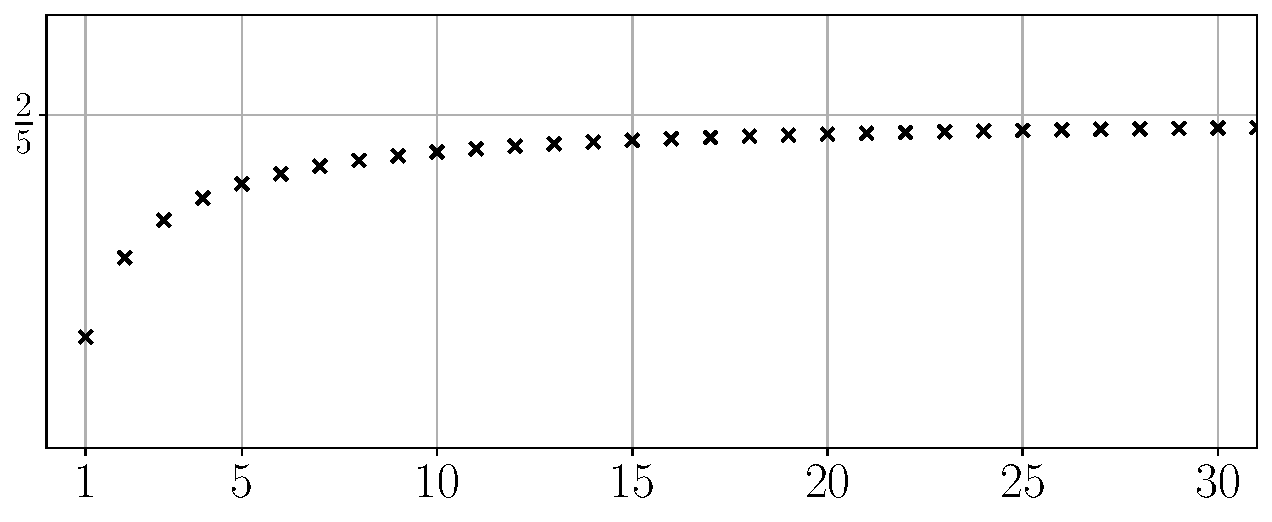
\includegraphics[width=\textwidth]{UA_Figures/UA_ex2_2_2_fig_a.pdf}
            \caption{\( \tfrac{2n + 1}{5n + 4} \) for \( 1 \leq n \leq 30 \)}
        \end{subfigure} \\
        \begin{subfigure}{0.75\textwidth}
            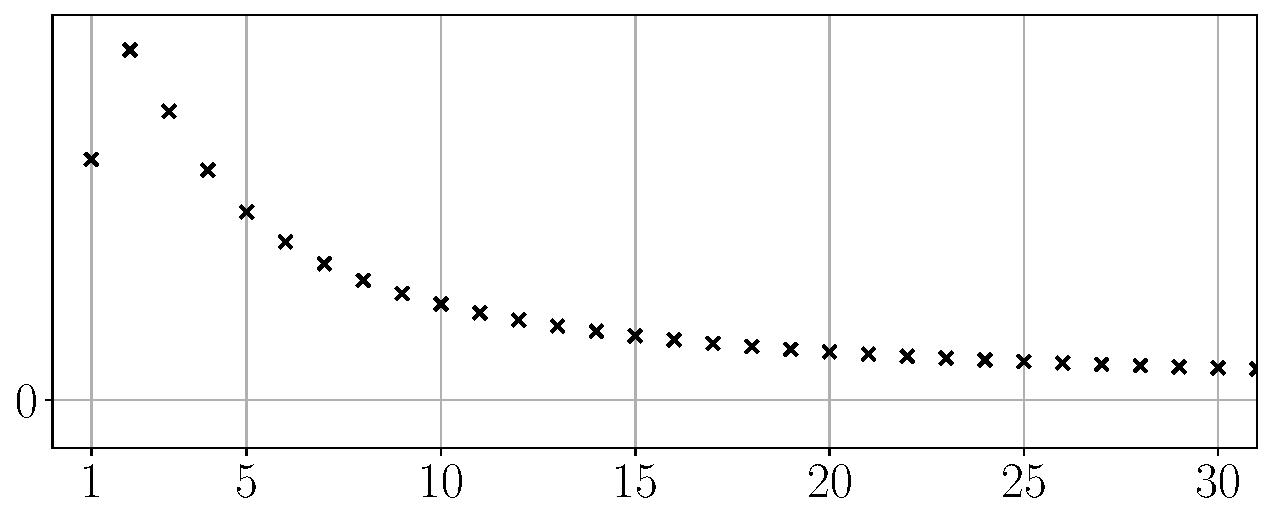
\includegraphics[width=\textwidth]{UA_Figures/UA_ex2_2_2_fig_b.pdf}
            \caption{\( \tfrac{2n^2}{n^3 + 3} \) for \( 1 \leq n \leq 30 \)}
        \end{subfigure} \\
        \begin{subfigure}{0.75\textwidth}
            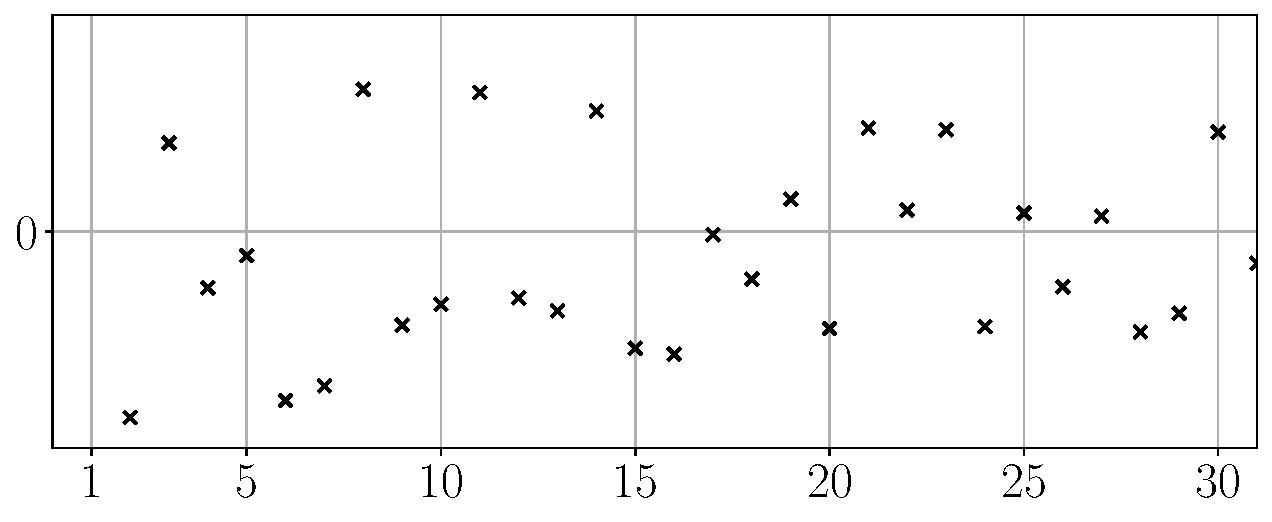
\includegraphics[width=\textwidth]{UA_Figures/UA_ex2_2_2_fig_c.pdf}
            \caption{\( \tfrac{\sin(n^2)}{\sqrt[3]{n}} \) for \( 1 \leq n \leq 30 \)}
        \end{subfigure}
        \caption{\Cref{ex:2.2.2} sequences for \( 1 \leq n \leq 30 \)}
        \label{fig:ex2.2.2}
    \end{figure}
\end{solution}

\begin{exercise}
\label{ex:2.2.3}
    Describe what we would have to demonstrate in order to disprove each of the following statements.
    \begin{enumerate}
        \item At every college in the United States, there is a student who is at least seven feet tall.

        \item For all colleges in the United States, there exists a professor who gives every student a grade of either A or B.

        \item There exists a college in the United States where every student is at least six feet tall.
    \end{enumerate}
\end{exercise}

\begin{solution}
    \begin{enumerate}
        \item We would have to find a college in the United States where every student is less than seven feet tall.

        \item We would have to find a college in the United States where each professor gives at least one student a grade of C or worse.

        \item We would have to show that every college in the United States has a student who is less than six feet tall.
    \end{enumerate}
\end{solution}

\begin{exercise}
\label{ex:2.2.4}
    Give an example of each or state that the request is impossible. For any that are impossible, give a compelling argument for why that is the case.
    \begin{enumerate}
        \item A sequence with an infinite number of ones that does not converge to one.

        \item A sequence with an infinite number of ones that converges to a limit not equal to one.

        \item A divergent sequence such that for every \( n \in \N \) it is possible to find \( n \) consecutive ones somewhere in the sequence.
    \end{enumerate}
\end{exercise}

\begin{solution}
    \begin{enumerate}
        \item Consider \( (x_n) = (1, 0, 1, 0, \ldots) \). This sequence has an infinite number of ones but, as shown in \Cref{ex:2.2.1}, diverges.

        \item This is impossible. Suppose \( (x_n) \) is such a sequence with \( \lim x_n = x \neq 1 \). Then there must exist some \( N \in \N \) such that for all \( n \geq N \) we have \( \abs{x_n - x} < \abs{1 - x} \). Since this sequence contains infinitely many ones, it must be the case that there is some \( m \geq N \) such that \( x_m = 1 \). This implies that \( \abs{x_m - x} = \abs{1 - x} < \abs{1 - x} \), which is a contradiction.

        \item Consider the sequence
        \[
            (x_n) = (1, 0, 1, 1, 0, 1, 1, 1, 0, 1, 1, 1, 1, 0, \ldots).
        \]
        For each \( n \in \N \) we can find \( n \) consecutive ones starting at the \( m \)\ts{th} position and, for \( n \geq 2 \), we can find a zero at the \( (m - 1) \)\ts{th} position, where \( m = \tfrac{n(n + 1)}{2} \). Furthermore, the sequence is divergent. To see this, suppose there was some \( x \in \R \) such that \( \lim x_n = x \). It follows that there is an \( N \in \N \) such that \( n \geq N \) implies that \( \abs{x_n - x} < \tfrac{1}{2} \). Since the sequence contains infinitely many ones and zeros, we can find indices \( k, \ell \geq N \) such that \( x_k = 1 \) and \( x_{\ell} = 0 \). Then
        \[
            1 = \abs{x_k - x_{\ell}} \leq \abs{x_k - x} + \abs{x_{\ell} - x} < \frac{1}{2} + \frac{1}{2} = 1,
        \]
        i.e., \( 1 < 1 \), which is a contradiction.
    \end{enumerate}
\end{solution}

\begin{exercise}
\label{ex:2.2.5}
    Let \( [[x]] \) be the greatest integer less than or equal to \( x \). For example, \( [[\pi]] = 3 \) and \( [[3]] = 3 \). For each sequence, find \( \lim a_n \) and verify it with the definition of convergence.
    \begin{enumerate}
        \item \( a_n = [[5/n]] \),

        \item \( a_n = [[(12 + 4n)/3n]] \).
    \end{enumerate}
    Reflecting on these examples, comment on the statement following Definition 2.2.3 that ``the smaller the \(\epsilon\)-neighborhood, the larger \( N \) may have to be."
\end{exercise}

\begin{solution}
    \begin{enumerate}
        \item We claim that \( \lim a_n = 0 \). Let \( \epsilon > 0 \) be given and observe that if \( n \geq 6 \), then
        \[
            0 < \frac{5}{n} < 1 \implies \bkt{\bkt{\frac{5}{n}}} = 0.
        \]
        So if we take \( N = 6 \), then \( n \geq N \) implies that \( \abs{\bkt{\bkt{\tfrac{5}{n}}}} = 0 < \epsilon \).

        \item We claim that \( \lim a_n = 1 \). Let \( \epsilon > 0 \) be given and observe that if \( n \geq 7 \), then
        \[
            \frac{1}{n} < \frac{1}{6} \iff \frac{4}{n} < \frac{2}{3} \iff \frac{4}{n} + \frac{1}{3} < 1.
        \]
        Hence for \( n \geq 7 \) we have
        \[
            0 < \frac{4}{n} + \frac{1}{3} < 1 \implies \bkt{\bkt{\frac{4}{n} + \frac{1}{3}}} = 0.
        \]
        So if we take \( N = 7 \), then \( n \geq N \) implies that
        \[
            \bkt{\bkt{\frac{12 + 4n}{3n} - 1}} = \bkt{\bkt{\frac{4}{n} + \frac{1}{3}}} = 0 < \epsilon.
        \]
    \end{enumerate}
    These examples demonstrate that taking smaller \(\epsilon\)-neighbourhoods may not require us to take larger values of \( N \); the same value of \( N \) in each example works for every \(\epsilon\)-neighbourhood that we choose.
\end{solution}

\begin{exercise}
\label{ex:2.2.6}
    Prove Theorem 2.2.7. To get started, assume \( (a_n) \to a \) and \( (a_n) \to b \). Now argue \( a = b \).
\end{exercise}

\begin{solution}
    Let \( \epsilon > 0 \) be given. There are positive integers \( N_1 \) and \( N_2 \) such that
    \[
        n \geq N_1 \implies \abs{a_n - a} < \frac{\epsilon}{2} \hspaceand[8mm] n \geq N_2 \implies \abs{a_n - b} < \frac{\epsilon}{2}.
    \]
    Let \( N = \max \{ N_1, N_2 \} \) and observe that for \( n \geq N \) we have
    \[
        \abs{a - b} = \abs{a - a_n + a_n - b} \leq \abs{a_n - a} + \abs{a_n - b} < \frac{\epsilon}{2} + \frac{\epsilon}{2} = \epsilon.
    \]
    So we have shown that \( \abs{a - b} < \epsilon \) for any \( \epsilon > 0 \); it follows from Theorem 1.2.6 that \( a = b \).
\end{solution}

\begin{exercise}
\label{ex:2.2.7}
    Here are two useful definitions:
    \begin{enumerate}[label = (\roman*)]
        \item A sequence \( (a_n) \) is \textit{eventually} in a set \( A \subseteq \R \) if there exists an \( N \in \N \) such that \( a_n \in A \) for all \( n \geq N \).

        \item A sequence \( (a_n) \) is \textit{frequently} in a set \( A \subseteq \R \) if, for every \( N \in \N \), there exists an \( n \geq N \) such that \( a_n \in A \).
        \begin{enumerate}
            \item Is the sequence \( (-1)^n \) eventually or frequently in the set \( \{ 1 \} \)?

            \item Which definition is stronger? Does frequently imply eventually or does eventually imply frequently?

            \item Give an alternate rephrasing of Definition 2.2.3B using either frequently or eventually. Which is the term we want?

            \item Suppose an infinite number of terms of a sequence \( (x_n) \) are equal to 2. Is \( (x_n) \) necessarily eventually in the interval \( (1.9, 2.1) \)? Is it frequently in \( (1.9, 2.1) \)?
        \end{enumerate}
    \end{enumerate}
\end{exercise}

\begin{solution}
    \begin{enumerate}
        \item The sequence \( (-1)^n \) is frequently but not eventually in the set \( \{ 1 \} \). To see this, let \( N \in \N \) be given. If \( N \) is even, then \( (-1)^N \in \{ 1 \} \) and \( (-1)^{N+1} \not\in \{ 1 \} \), and if \( N \) is odd then \( (-1)^N \not\in \{ 1 \} \) and \( (-1)^{N+1} \in \{ 1 \} \). In any case, we can always find indices \( m, n \geq N \) such that \( (-1)^m \not\in \{ 1 \} \) (this shows that the sequence is not eventually in \( \{ 1 \} \)) and such that \( (-1)^n \in \{ 1 \} \) (this shows that the sequence is frequently in \( \{ 1 \} \)).

        \item Eventually is the stronger definition. Frequently does not imply eventually, as part (a) shows, but eventually does imply frequently. To see this, suppose that \( (a_n) \) is eventually in a set \( A \), i.e., there is an \( N \in \N \) such that \( a_n \in A \) for all \( n \geq N \). Let \( M \in \N \) be given. Set \( n = \max \{ M, N \} \) and observe that \( n \geq M \) and \( a_n \in A \). Hence \( (a_n) \) is frequently in \( A \).

        \item The term we want is eventually. Here is a rephrasing of Definition 2.2.3B: a sequence \( (a_n) \) converges to \( a \) if, given any \( \epsilon > 0 \), the sequence \( (a_n) \) is eventually in the \( \epsilon \)-neighbourhood \( V_{\epsilon}(a) \) of \( a \).

        \item Such a sequence is not necessarily eventually in \( (1.9, 2.1) \); consider the sequence \( (x_n) = (2, 0, 2, 0, 2, \ldots) \) for example. For any \( N \in \N \), we can always find an index \( n \geq N \) (either \( n = N \) or \( n = N + 1 \)) such that \( x_n = 0 \not\in (1.9, 2.1) \). However, such a sequence must be frequently in \( (1.9, 2.1) \). To see this, let \( N \in \N \) be given. Then there must exist an index \( n \geq N \) such that \( x_n = 2 \in (1.9, 2.1) \) (otherwise there would be only finitely many twos in the sequence).
    \end{enumerate}
\end{solution}

\begin{exercise}
\label{ex:2.2.8}
    For some additional practice with nested quantifiers, consider the following invented defintion:

    Let's call a sequence \( (x_n) \) \textit{zero-heavy} if there exists \( M \in \N \) such that for all \( N \in \N \) there exists \( n \) satisfying \( N \leq n \leq N + M \) where \( x_n = 0 \).
    \begin{enumerate}
        \item Is the sequence \( (0, 1, 0, 1, 0, 1, \ldots) \) zero-heavy?

        \item If a sequence is zero-heavy does it necessarily contain an infinite number of zeros? If not, provide a counterexample.

        \item If a sequence contains an infinite number of zeros, is it necessarily zero-heavy? If not, provide a counterexample.

        \item Form the logical negation of the above definition. That is, complete the sentence: A sequence is \textit{not} zero-heavy if ....
    \end{enumerate}
\end{exercise}

\begin{solution}
    \begin{enumerate}
        \item This sequence is zero-heavy; \( M = 1 \) works. Indeed, let \( N \in \N \) be given. If \( N \) is odd then let \( n = N \) and if \( N \) is even then let \( n = N + 1 \). In either case, we have \( N \leq n \leq N + 1 \) and \( x_n = 0 \).

        \item A zero-heavy sequence must contain an infinite number of zeros. To see this, suppose \( (x_n) \) is a sequence with a finite number of zeros, i.e.\ there is an \( N \in \N \) such that \( x_n \neq 0 \) for all \( n \geq N \). Then no matter which \( M \) we choose, we will never be able to find \( n \in \N \) with \( N \leq n \leq N + M \) and \( x_n = 0 \). Thus the sequence \( (x_n) \) is not zero-heavy.

        \item A sequence with an infinite number of zeros is not necessarily zero-heavy. For a counterexample, consider the sequence
        \[
            (x_n) = (1, 0, 1, 1, 0, 1, 1, 1, 0, 1, 1, 1, 1, 0, \ldots).
        \]
        This sequence contains infinitely many zeros, but is not zero-heavy. To see this, let \( M \in \N \) be given. It is always possible to find \( M \) consecutive ones in the sequence \( (x_n) \) (see \Cref{ex:2.2.4} (c)); suppose this string of ones starts at \( x_N = 1 \). Then for each \( n \in \N \) satisfying \( N \leq n \leq N + M \), we have \( x_n = 1 \neq 0 \).

        \item A sequence is not zero-heavy if for every \( M \in \N \) there exists an \( N \in \N \) such that \( x_n \neq 0 \) for each \( n \in \N \) satisfying \( N \leq n \leq N + M \).
    \end{enumerate}
\end{solution}

\section{The Algebraic and Order Limit Theorems}
\label{sec:2.3}

\begin{exercise}
\label{ex:2.3.1}
    Let \( x_n \geq 0 \) for all \( n \in \N \).
    \begin{enumerate}
        \item If \( (x_n) \to 0 \), show that \( ( \sqrt{x_n} ) \to 0 \).

        \item If \( (x_n) \to x \), show that \( ( \sqrt{x_n} ) \to \sqrt{x} \).
    \end{enumerate}
\end{exercise}

\begin{solution}
    \begin{enumerate}
        \item Let \( \epsilon > 0 \) be given. Since \( x_n \to 0 \), there exists an \( N \in \N \) such that
        \[
            n \geq N \implies \abs{x_n} = x_n < \epsilon^2 \iff \sqrt{x_n} < \epsilon.
        \]
        It follows that \( \lim \paren{\sqrt{x_n}} = 0 \).

        \item By Theorem 2.3.4, we must have \( x \geq 0 \). The case \( x = 0 \) was handled in part (a), so suppose that \( x > 0 \), which gives \( \sqrt{x} > 0 \). For each \( n \in \N \), observe that
        \[
            \abs{\sqrt{x_n} - \sqrt{x}} = \frac{\abs{\sqrt{x_n} - \sqrt{x}} \paren{ \sqrt{x_n} + \sqrt{x} }}{\sqrt{x_n} + \sqrt{x}} = \frac{\abs{x_n - x}}{\sqrt{x_n} + \sqrt{x}} \leq \frac{\abs{x_n - x}}{\sqrt{x}}.
        \]
        Let \( \epsilon > 0 \) be given. Since \( x_n \to x \), there exists an \( N \in \N \) such that \( \abs{x_n - x} < \epsilon \sqrt{x} \) whenever \( n \geq N \). For \( n \geq N \), it follows that
        \[
            \abs{\sqrt{x_n} - \sqrt{x}} \leq \frac{\abs{x_n - x}}{\sqrt{x}} < \epsilon.
        \]
        Thus \( \lim \paren{ \sqrt{x_n} } = \sqrt{x} \).
    \end{enumerate}
\end{solution}

\begin{exercise}
\label{ex:2.3.2}
    Using only Definition 2.2.3, prove that if \( (x_n) \to 2 \) then
    \begin{enumerate}
        \item \( \paren{ \frac{2 x_n - 1}{3} } \to 1 \);

        \item \( (1/x_n) \to 1/2 \).
    \end{enumerate}
\end{exercise}

\begin{solution}
    \begin{enumerate}
        \item Let \( \epsilon > 0 \) be given. Since \( x_n \to 2 \), there exists an \( N \in \N \) such that \( n \geq N \) implies that \( \abs{x_n - 2} < \tfrac{3 \epsilon}{2} \). For \( n \geq N \) we then have
        \[
            \abs{\frac{2 x_n - 1}{3} - 1} = \abs{\frac{2 x_n - 4}{3}} = \frac{2}{3} \abs{x_n - 2} < \epsilon.
        \]
        It follows that \( \paren{ \frac{2 x_n - 1}{3} } \to 1 \).

        \item Since \( x_n \to 2 \), there is an \( N_1 \in \N \) such that \( n \geq N_1 \implies \abs{x_n - 2} < 1 \). For \( n \geq N_1 \) we then have
        \[
            2 \leq \abs{x_n - 2} + \abs{x_n} < 1 + \abs{x_n} \implies 1 < \abs{x_n} \implies \frac{1}{\abs{x_n}} < 1.
        \]
        Let \( \epsilon > 0 \) be given. Since \( x_n \to 2 \), there is an \( N_2 \in \N \) such that \( \abs{x_n - 2} < 2 \epsilon \) whenever \( n \geq N_2 \). Set \( N = \max \{ N_1, N_2 \} \) and observe that for \( n \geq N \) we have
        \[
            \abs{\frac{1}{x_n} - \frac{1}{2}} = \abs{\frac{2 - x_n}{2 x_n}} = \frac{\abs{x_n - 2}}{2 \abs{x_n}} < \frac{\abs{x_n - 2}}{2} < \epsilon.
        \]
        It follows that \( \tfrac{1}{x_n} \to \tfrac{1}{2} \).
    \end{enumerate}
\end{solution}

\begin{exercise}[Squeeze Theorem]
\label{ex:2.3.3}
    Show that if \( x_n \leq y_n \leq z_n \) for all \( n \in \N \), and if \( \lim x_n = \lim z_n = l \), then \( \lim y_n = l \) as well.
\end{exercise}

\begin{solution}
    Let \( \epsilon > 0 \) be given. There are positive integers \( N_1 \) and \( N_2 \) such that
    \begin{gather*}
        n \geq N_1 \implies \abs{x_n - l} < \epsilon \iff -\epsilon < x_n - l < \epsilon, \\[2mm]
        n \geq N_2 \implies \abs{z_n - l} < \epsilon \iff -\epsilon < z_n - l < \epsilon.
    \end{gather*}
    Let \( N = \max \{ N_1, N_2 \} \). Then since \( x_n - l \leq y_n - l \leq z_n - l \) for all \( n \in \N \), for \( n \geq N \) we have
    \[
        -\epsilon < y_n - l < \epsilon \iff \abs{y_n - l} < \epsilon.
    \]
    It follows that \( \lim y_n = l \).
\end{solution}

\begin{exercise}
\label{ex:2.3.4}
    Let \( (a_n) \to 0 \), and use the Algebraic Limit Theorem to compute each of the following limits (assuming the fractions are always defined):
    \begin{enumerate}
        \item \( \lim \paren{ \frac{1 + 2 a_n}{1 + 3 a_n - 4 a_n^2} } \)

        \item \( \lim \paren{ \frac{(a_n + 2)^2 - 4}{a_n} } \)

        \item \( \lim \paren{ \frac{\frac{2}{a_n} + 3}{\frac{1}{a_n} + 5} } \).
    \end{enumerate}
\end{exercise}

\begin{solution}
    The manipulations of limits in these solutions are justified by the Algebraic Limit Theorem (Theorem 2.3.3).
    \begin{enumerate}
        \item We have
        \[
            \lim \paren{ \frac{1 + 2 a_n}{1 + 3 a_n - 4 a_n^2} } = \frac{1 + 2 \lim a_n}{1 + 3 \lim a_n - 4 (\lim a_n)^2} = \frac{1}{1} = 1.
        \]

        \item We have
        \[
            \lim \paren{ \frac{(a_n + 2)^2 - 4}{a_n} } = \lim \paren{ \frac{a_n^2 + 4 a_n}{a_n} } = \lim (a_n + 4) = \lim a_n + 4 = 4.
        \]

        \item We have
        \[
            \lim \paren{ \frac{\frac{2}{a_n} + 3}{\frac{1}{a_n} + 5} } = \lim \paren{ \frac{2 + 3 a_n}{1 + 5 a_n} } = \frac{2 + 3 \lim a_n}{1 + 5 \lim a_n} = \frac{2}{1} = 2.
        \]
    \end{enumerate}
\end{solution}

\begin{exercise}
\label{ex:2.3.5}
    Let \( (x_n) \) and \( (y_n) \) be given, and define \( (z_n) \) to be the ``shuffled" sequence \( (x_1, y_1, x_2, y_2, x_3, y_3, \ldots, x_n, y_n, \ldots) \). Prove that \( (z_n) \) is convergent if and only if \( (x_n) \) and \( (y_n) \) are both convergent with \( \lim x_n = \lim y_n \).
\end{exercise}

\begin{solution}
    \( (z_n) \) is the sequence given by
    \[
        z_n = \begin{cases}
            x_{\frac{n + 1}{2}} & \text{if } n \text{ is odd}, \\
            y_{\frac{n}{2}} & \text{if } n \text{ is even}.
        \end{cases}
    \]
    Suppose that \( (x_n) \) and \( (y_n) \) are both convergent with \( \lim x_n = \lim y_n = L \) for some \( L \in \R \) and let \( \epsilon > 0 \) be given. There are positive integers \( N_1 \) and \( N_2 \) such that
    \[
        n \geq N_1 \implies \abs{x_n - L} < \epsilon \hspaceand[8mm] n \geq N_2 \implies \abs{y_n - L} < \epsilon.
    \]
    Let \( N = \max \{ N_1, N_2 \} \) and suppose \( n \in \N \) is such that \( n \geq 2N \). If \( n \) is odd then \( \frac{n + 1}{2} \in \N \) and
    \[
        n \geq 2N > 2N - 1 \implies \frac{n + 1}{2} > N \geq N_1 \implies \abs{x_{\frac{n + 1}{2}} - L} < \epsilon.
    \]
    Hence
    \[
        \abs{z_n - L} = \abs{x_{\frac{n + 1}{2}} - L} < \epsilon.
    \]
    If \( n \) is even then \( \frac{n}{2} \in \N \) and
    \[
        n \geq 2N \implies \frac{n}{2} \geq N \geq N_2 \implies \abs{y_{\frac{n}{2}} - L} < \epsilon.
    \]
    Hence
    \[
        \abs{z_n - L} = \abs{y_{\frac{n}{2}} - L} < \epsilon.
    \]
    In either case we have \( \abs{z_n - L} < \epsilon \), i.e.,
    \[
        n \geq 2N \implies \abs{z_n - L} < \epsilon.
    \]
    It follows that \( \lim z_n = L \).
    
    Now suppose that \( (z_n) \) is convergent with \( \lim z_n = L \) for some \( L \in \R \). Let \( \epsilon > 0 \) be given. Since \( z_n \to L \), there exists an \( N \in \N \) such that \( \abs{z_n - L} < \epsilon \) whenever \( n \geq N \). For such \( n \), we have \( 2n > 2n - 1 \geq n \geq N \) and so
    \[
        \abs{x_n - L} = \abs{z_{2n - 1} - L} < \epsilon \hspaceand[8mm] \abs{y_n - L} = \abs{z_{2n} - L} < \epsilon.
    \]
    It follows that \( \lim x_n = \lim y_n = L \).
\end{solution}

\begin{exercise}
\label{ex:2.3.6}
    Consider the sequence given by \( b_n = n - \sqrt{n^2 + 2n} \). Taking \( (1/n) \to 0 \) as given, and using both the Algebraic Limit Theorem and the result in \Cref{ex:2.3.1}, show \( \lim b_n \) exists and find the value of the limit.
\end{exercise}

\begin{solution}
    Observe that
    \[
        b_n = n - \sqrt{n^2 + 2n} = \frac{(n - \sqrt{n^2 + 2n})(n + \sqrt{n^2 + 2n})}{n + \sqrt{n^2 + 2n}} = \frac{-2n}{n + \sqrt{n^2 + 2n}} = \frac{-2}{1 + \sqrt{1 + \tfrac{2}{n}}}.
    \]
    Hence, using \Cref{ex:2.3.1},
    \[
        \lim b_n = \lim \paren{ \frac{-2}{1 + \sqrt{1 + \tfrac{2}{n}}} } = \frac{-2}{1 + \sqrt{1 + 2 \lim \tfrac{1}{n} }} = \frac{-2}{1 + \sqrt{1}} = -1.
    \]
    \Cref{fig:ex2.3.6} shows a graph of the first thirty terms of this sequence.
    \begin{figure}
        \centering
        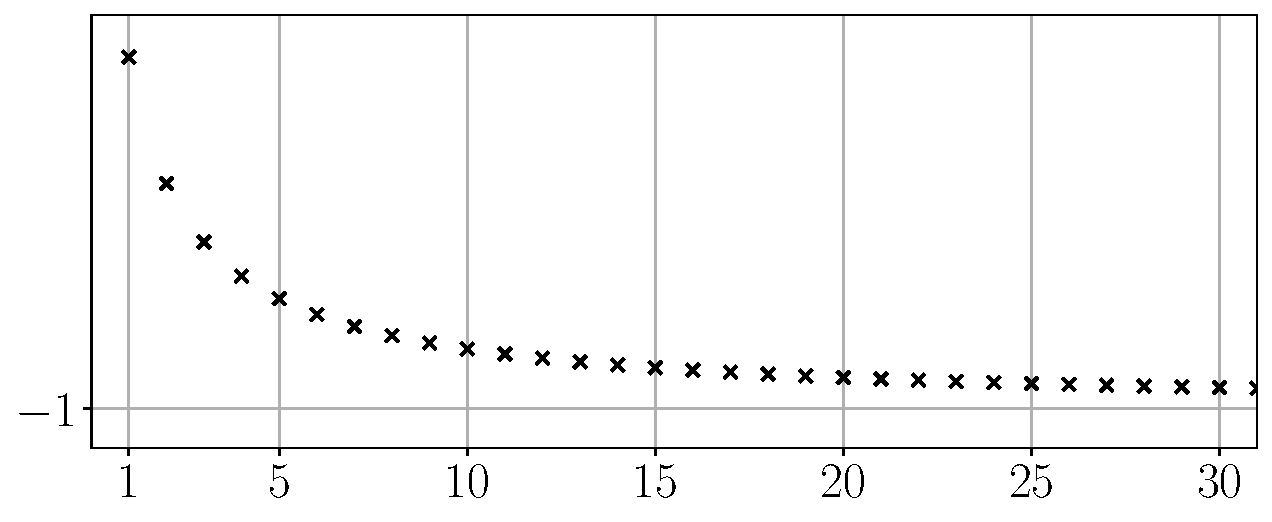
\includegraphics[width=0.8\textwidth]{UA_Figures/UA_ex2_3_6_fig.pdf}
        \caption{\( b_n = n - \sqrt{n^2 + 2n} \) for \( 1 \leq n \leq 30 \)}
        \label{fig:ex2.3.6}
    \end{figure}
\end{solution}

\begin{exercise}
\label{ex:2.3.7}
    Give an example of each of the following, or state that such a request is impossible by referencing the proper theorem(s):
    \begin{enumerate}
        \item sequences \( (x_n) \) and \( (y_n) \), which both diverge, but whose sum \( (x_n + y_n) \) converges;

        \item sequences \( (x_n) \) and \( (y_n) \), where \( (x_n) \) converges, \( (y_n) \) diverges, and \( (x_n + y_n) \) converges;

        \item a convergent sequence \( (b_n) \) with \( b_n \neq 0 \) for all \( n \) such that \( (1/b_n) \) diverges;

        \item an unbounded sequence \( (a_n) \) and a convergent sequence \( (b_n) \) with \( (a_n - b_n) \) bounded;

        \item two sequences \( (a_n) \) and \( (b_n) \), where \( (a_n b_n) \) and \( (a_n) \) converge but \( (b_n) \) does not.
    \end{enumerate}
\end{exercise}

\begin{solution}
    \begin{enumerate}
        \item Take \( x_n = n \) and \( y_n = -n \).

        \item This is impossible. If \( (x_n) \) and \( (x_n + y_n) \) both converge, then by the Algebraic Limit Theorem (Theorem 2.3.3) \( (y_n) \) must be convergent with limit \( \lim y_n = \lim (x_n + y_n) - \lim x_n \).

        \item Take \( b_n = \tfrac{1}{n} \).

        \item This is impossible; \( (a_n - b_n) \) must be unbounded. Since \( (b_n) \) is convergent, it must be bounded (Theorem 2.3.2), i.e., there exists some \( B \geq 0 \) such that \( \abs{b_n} \leq B \) for all \( n \in \N \). Let \( M \geq 0 \) be given. Since \( (a_n) \) is unbounded, there exists some \( N \in \N \) such that \( \abs{a_N} \geq M + B \). Then observe that
        \[
            \abs{a_N - b_N} \geq \abs{\abs{a_N} - \abs{b_N}} \geq \abs{a_N} - \abs{b_N} \geq M + B - B = M,
        \]
        where we have used \Cref{ex:1.2.6} (d) for the first inequality. Since \( M \) was arbitrary, we see that the sequence \( (a_n - b_n) \) is unbounded.

        \item Take \( a_n = \tfrac{1}{n^2} \) and \( b_n = n \).
    \end{enumerate}
\end{solution}

\begin{exercise}
\label{ex:2.3.8}
    Let \( (x_n) \to x \) and let \( p(x) \) be a polynomial.
    \begin{enumerate}
        \item Show \( p(x_n) \to p(x) \).

        \item Find an example of a function \( f(x) \) and a convergent sequence \( (x_n) \to x \) where the sequence \( f(x_n) \) converges, but not to \( f(x) \).
    \end{enumerate}
\end{exercise}

\begin{solution}
    \begin{enumerate}
        \item Suppose \( p(x) = a_m x^m + a_{m-1} x^{m-1} + \cdots + a_1 x + a_0 \). The Algebraic Limit Theorem (Theorem 2.3.3) and some simple induction arguments allow us to make the following manipulations:
        \begin{align*}
            \lim (p(x_n)) &= \lim (a_m x_n^m + a_{m-1} x_n^{m-1} + \cdots + a_1 x_n + a_0) \\[2mm]
            &= a_m (\lim x_n)^m + a_{m-1} (\lim x_n)^{m-1} + \cdots + a_1 \lim x_n + a_0 \\[2mm]
            &= a_m x^m + a_{m-1} x^{m-1} + \cdots + a_1 x + a_0 \\[2mm]
            &= p(x).
        \end{align*}

        \item Consider the function \( f : \R \to \R \) given by
        \[
            f(x) = \begin{cases}
                0 & \text{if } x = 0, \\
                1 & \text{otherwise},
            \end{cases}
        \]
        and the convergent sequence \( x_n = \tfrac{1}{n} \to 0 \). We then have \( (f(x_n)) = (1, 1, 1, \ldots) \), which converges to \( 1 \neq 0 = f(0) \).
    \end{enumerate}
\end{solution}

\begin{exercise}
\label{ex:2.3.9}
    \begin{enumerate}
        \item Let \( (a_n) \) be a bounded (not necessarily convergent) sequence, and assume \( \lim b_n = 0 \). Show that \( \lim (a_n b_n) = 0 \). Why are we not allowed to use the Algebraic Limit Theorem to prove this?

        \item Can we conclude anything about the convergence of \( (a_n b_n) \) if we assume that \( (b_n) \) converges to some nonzero limit \( b \)?

        \item Use (a) to prove Theorem 2.3.3, part (iii), for the case when \( a = 0 \).
    \end{enumerate}
\end{exercise}

\begin{solution}
    \begin{enumerate}
        \item There is an \( M > 0 \) such that \( \abs{a_n} \leq M \) for all \( n \in \N \). Let \( \epsilon > 0 \) be given. Since \( b_n \to 0 \), there is an \( N \in \N \) such that
        \[
            n \geq N \implies \abs{b_n} < \frac{\epsilon}{M}.
        \]
        Observe that for \( n \geq N \) we have
        \[
            \abs{a_n b_n} = \abs{a_n} \abs{b_n} \leq M \abs{b_n} < \frac{M \epsilon}{M} = \epsilon.
        \]
        It follows that \( \lim (a_n b_n) = 0 \). We may not use the Algebraic Limit Theorem here since the sequence \( (a_n) \) is not necessarily convergent; the hypotheses of that theorem require both sequences \( (a_n) \) and \( (b_n) \) to be convergent.

        \item If the sequence \( (a_n) \) converges to some \( a \) then we may use the Algebraic Limit Theorem to conclude that \( \lim (a_n b_n) = ab \). If the sequence \( (a_n) \) is divergent, then \( (a_n b_n) \) must also be divergent. To see this, we will prove the contrapositive, i.e., if \( (a_n b_n) \) converges to some \( x \in \R \) then \( (a_n) \) is convergent. Indeed, since \( b \neq 0 \), the Algebraic Limit Theorem implies that
        \[
            \lim a_n = \lim \paren{ \frac{a_n b_n}{b_n} } = \frac{x}{b}.
        \]

        \item Since \( (b_n) \) is convergent, it is bounded (Theorem 2.3.2). So we may apply part (a) (we have swapped the roles of \( (a_n) \) and \( (b_n) \)) to conclude that
        \[
            \lim (a_n b_n) = 0 = 0b = ab.
        \]
    \end{enumerate}
\end{solution}

\begin{exercise}
\label{ex:2.3.10}
    Consider the following list of conjectures. Provide a short proof for those that are true and a counterexample for any that are false.
    \begin{enumerate}
        \item If \( \lim (a_n - b_n) = 0 \), then \( \lim a_n = \lim b_n \).

        \item If \( (b_n) \to b \), then \( \abs{b_n} \to \abs{b} \).

        \item If \( (a_n) \to a \) and \( (b_n - a_n) \to 0 \), then \( (b_n) \to a \).

        \item If \( (a_n) \to 0 \) and \( \abs{b_n - b} \leq a_n \) for all \( n \in \N \), then \( (b_n) \to b \).
    \end{enumerate}
\end{exercise}

\begin{solution}
    \begin{enumerate}
        \item This is false; consider \( a_n = b_n = (-1)^n \).

        \item This is true. Let \( \epsilon > 0 \) be given. Since \( b_n \to b \), there is an \( N \in \N \) such that \( \abs{b_n - b} < \epsilon \) whenever \( n \geq N \). For such \( n \), the reverse triangle inequality (\Cref{ex:1.2.6} (d)) gives
        \[
            \abs{\abs{b_n} - \abs{b}} \leq \abs{b_n - b} < \epsilon.
        \]
        It follows that \( \lim \abs{b_n} = \abs{b} \).

        \item This is true. Using the Algebraic Limit Theorem (Theorem 2.3.3), we have
        \[
            \lim b_n = \lim (b_n - a_n + a_n) = \lim (b_n - a_n) + \lim a_n = 0 + a = a.
        \]

        \item This is true. Since \( 0 \leq \abs{b_n - b} \leq a_n \) for every \( n \in \N \), the Squeeze Theorem (\Cref{ex:2.3.3}) implies that \( \lim \abs{b_n - b} = 0 \), i.e., for every \( \epsilon > 0 \) there is an \( N \in \N \) such that
        \[
            n \geq N \implies \abs{\abs{b_n - b} - 0} = \abs{b_n - b} < \epsilon,
        \]
        which is exactly the statement \( \lim b_n = b \).
    \end{enumerate}
\end{solution}

\begin{exercise}[Cesaro Means]
\label{ex:2.3.11}
    \begin{enumerate}
        \item Show that if \( (x_n) \) is a convergent sequence, then the sequence given by the averages
        \[
            y_n = \frac{x_1 + x_2 + \cdots + x_n}{n}
        \]
        also converges to the same limit.

        \item Give an example to show that it is possible for the sequence \( (y_n) \) of averages to converge even if \( (x_n) \) does not.
    \end{enumerate}
\end{exercise}

\begin{solution}
    \begin{enumerate}
        \item Suppose \( \lim x_n = x \) and let \( \epsilon > 0 \) be given. Since \( x_n \to x \), there is a positive integer \( N_1 \in \N \) such that
        \[
            n \geq N_1 \implies \abs{x_n - x} < \frac{\epsilon}{2}.
        \]
        Given this \( N_1 \), notice that the sequence
        \[
            \paren{ \frac{\abs{x_1 - x} + \cdots + \abs{x_{N_1} - x}}{n} }_{n=1}^{\infty}
        \]
        has non-negative terms and converges to zero (the numerator is a constant); it follows that there is an \( N_2 \in \N \) such that
        \[
            n \geq N_2 \implies \frac{\abs{x_1 - x} + \cdots + \abs{x_{N_1} - x}}{n} < \frac{\epsilon}{2}.
        \]
        Set \( N = \max \{ N_1, N_2 \} \) and observe that for \( n \geq N + 1 \) we have
        \begin{align*}
            \abs{y_n - x} &= \abs{\frac{x_1 + \cdots + x_n}{n} - \frac{nx}{n}} \\[2mm]
            &= \abs{\frac{(x_1 - x) + \cdots + (x_n - x)}{n}} \\[2mm]
            &\leq \frac{\abs{x_1 - x} + \cdots + \abs{x_{N_1} - x}}{n} + \frac{\abs{x_{N_1 + 1} - x} + \cdots + \abs{x_n - x}}{n} \\[2mm]
            &< \frac{\epsilon}{2} + \frac{n - N_1}{n} \cdot \frac{\epsilon}{2} \\[2mm]
            &\leq \frac{\epsilon}{2} + \frac{\epsilon}{2} \\[2mm]
            &= \epsilon.
        \end{align*}
        It follows that \( \lim y_n = x \).

        \item Consider the divergent sequence \( x_n = (-1)^{n+1} \). The sequence of averages \( (y_n) \) is then
        \[
            y_n = \begin{cases}
                \frac{1}{n} & \text{if } n \text{ is odd}, \\
                0 & \text{if } n \text{ is even},
            \end{cases}
        \]
        which satisfies \( \lim y_n = 0 \).
    \end{enumerate}
\end{solution}

\begin{exercise}
\label{ex:2.3.12}
    A typical task in analysis is to decipher whether a property possessed by every term in a convergent sequence is necessarily  inherited by the limit. Assume \( (a_n) \to a \), and determine the validity of each claim. Try to produce a counterexample for any that are false.
    \begin{enumerate}
        \item If every \( a_n \) is an upper bound for a set \( B \), then \( a \) is also an upper bound for \( B \).

        \item If every \( a_n \) is in the complement of the interval \( (0, 1) \), then \( a \) is also in the complement of \( (0, 1) \).

        \item If every \( a_n \) is rational, then \( a \) is rational.
    \end{enumerate}
\end{exercise}

\begin{solution}
    \begin{enumerate}
        \item This is true. For any \( b \in B \) we have \( b \leq a_n \) for all \( n \in \N \); the Order Limit Theorem (Theorem 2.3.4) then implies that \( b \leq a \) and it follows that \( a \) is an upper bound for \( B \).

        \item This is true. Observe that for a real number \( x \) we have
        \[
            x \not\in (0, 1) \iff x \leq 0 \text{ or } x \geq 1 \iff \abs{x - \frac{1}{2}} \geq \frac{1}{2}.
        \]
        So for each \( n \in \N \) we have \( \abs{a_n - \tfrac{1}{2}} \geq \tfrac{1}{2} \). The Algebraic Limit Theorem (Theorem 2.3.3) and \Cref{ex:2.3.10} (b) imply that \( \lim \abs{a_n - \tfrac{1}{2}} = \abs{a - \tfrac{1}{2}} \), and hence the Order Limit Theorem (Theorem 2.3.4) implies that \( \abs{a - \tfrac{1}{2}} \geq \tfrac{1}{2} \). It follows that \( a \) belongs to the complement of \( (0, 1) \).

        \item This is false. By the density of \( \Q \) in \( \R \) (Theorem 1.4.3), for each \( n \in \N \) we may pick a rational number \( a_n \) satisfying \( \sqrt{2} < a_n < \sqrt{2} + \tfrac{1}{n} \). The Squeeze Theorem (\Cref{ex:2.3.3}) then implies that \( \lim a_n = \sqrt{2} \), which is an irrational number.
    \end{enumerate}
\end{solution}

\begin{exercise}[Iterated Limits]
\label{ex:2.3.13}
    Given a doubly indexed array \( a_{mn} \) where \( m, n \in \N \), what should \( \lim_{m, n \to \infty} a_{mn} \) represent?
    \begin{enumerate}
        \item Let \( a_{mn} = m/(m + n) \) and compute the \textit{iterated} limits
        \[
            \lim_{n \to \infty} \paren{ \lim_{m \to \infty} a_{mn} } \hspaceand[8mm] \lim_{m \to \infty} \paren{ \lim_{n \to \infty} a_{mn} }.
        \]
        Define \( \lim_{m, n \to \infty} a_{mn} = a \) to mean that for all \( \epsilon > 0 \) there exists an \( N \in \N \) such that if both \( m, n \geq N \), then \( \abs{a_{mn} - a} < \epsilon \).

        \item Let \( a_{mn} = 1/(m + n) \). Does \( \lim_{m, n \to \infty} a_{mn} \) exist in this case? Do the two iterated limits exist? How do these three values compare? Answer these same questions for \( a_{mn} = mn/(m^2 + n^2) \).

        \item Produce an example where \( \lim_{m, n \to \infty} a_{mn} \) exists but where neither iterated limit can be computed.

        \item Assume \( \lim_{m, n \to \infty} a_{mn} = a \), and assume that for each fixed \( m \in \N \), \( \lim_{n \to \infty} (a_{mn}) = b_m \). Show \( \lim_{m \to \infty} b_m = a \).

        \item Prove that if \( \lim_{m, n \to \infty} a_{mn} \) exists and the iterated limits both exist, then all three limits must be equal.
    \end{enumerate}
\end{exercise}

\begin{solution}
    \begin{enumerate}
        \item We apply the Algebraic Limit Theorem (Theorem 2.3.3):
        \[
            \lim_{m \to \infty} a_{mn} = \lim_{m \to \infty} \paren{ \frac{m}{m + n} } = \lim_{m \to \infty} \paren{ \frac{1}{1 + \frac{n}{m}} } = \frac{1}{1 + n \lim_{m \to \infty} \paren{ \frac{1}{m} }} = \frac{1}{1} = 1.
        \]
        Hence \( \lim_{n \to \infty} \paren{ \lim_{m \to \infty} a_{mn} } = \lim_{n \to \infty} (1) = 1 \). Similarly,
        \[
            \lim_{n \to \infty} a_{mn} = \lim_{n \to \infty} \paren{ \frac{m}{m + n} } = \lim_{n \to \infty} \paren{ \frac{\frac{m}{n}}{1 + \frac{m}{n}} } = \frac{m \lim_{n \to \infty} \paren{ \frac{1}{n} }}{1 + m \lim_{n \to \infty} \paren{ \frac{1}{n} }} = \frac{0}{1} = 0.
        \]
        Thus \( \lim_{m \to \infty} \paren{ \lim_{n \to \infty} a_{mn} } = \lim_{m \to \infty} (0) = 0 \).

        \item For \( a_{mn} = \tfrac{1}{m + n} \), we have \( \lim_{m, n \to \infty} a_{mn} = 0 \). To see this, let \( \epsilon > 0 \) be given. There is an \( N \in \N \) such that \( \tfrac{1}{n} < \epsilon \) whenever \( n \geq N \), so that for \( m, n \geq N \) we have
        \[
            \abs{a_{mn}} = \frac{1}{m + n} < \frac{1}{n} < \epsilon.
        \]
        Thus \( \lim_{m, n \to \infty} a_{mn} = 0 \). The two iterated limits also exist and are equal to 0. Indeed, observe that for all \( m, n \in \N \) we have \( 0 < \tfrac{1}{m + n} < \tfrac{1}{m} \). The Squeeze Theorem (\Cref{ex:2.3.3}) then implies that \( \lim_{m \to \infty} a_{mn} = \lim_{m \to \infty} \tfrac{1}{m + n} = 0 \) and it follows that \( \lim_{n \to \infty} \paren{ \lim_{m \to \infty} a_{mn} } = \lim_{n \to \infty} (0) = 0 \). A similar argument shows that \( \lim_{m \to \infty} \paren{ \lim_{n \to \infty} a_{mn} } = 0 \).

        Now let \( a_{mn} = \tfrac{mn}{m^2 + n^2} \); we claim that \( \lim_{m, n \to \infty} a_{mn} \) does not exist. To see this, let us seek a contradiction and suppose that \( \lim_{m, n \to \infty} a_{mn} = x \) for some \( x \in \R \). There then exists an \( N \in \N \) such that \( \abs{a_{mn} - x} < \tfrac{1}{20} \) whenever \( m, n \geq N \). In particular, taking \( n = m \),
        \[
            m \geq N \implies \abs{\frac{m^2}{m^2 + m^2} - x} = \abs{\frac{1}{2} - x} < \frac{1}{20} \iff x \in \paren{ \frac{9}{20}, \frac{11}{20} }.
        \]
        Similarly, taking \( n = 2m \),
        \[
            m \geq N \implies \abs{\frac{2m^2}{m^2 + 4m^2} - x} = \abs{\frac{2}{5} - x} < \frac{1}{20} \iff x \in \paren{ \frac{7}{20}, \frac{9}{20} }.
        \]
        So assuming that \( \lim_{m, n \to \infty} a_{mn} = x \) for some \( x \in \R \) leads us to the contradiction that \( x < \tfrac{9}{20} \) and \( x > \tfrac{9}{20} \); it follows that \( \lim_{m, n \to \infty} a_{mn} \) does not exist. However, the two iterated limits do exist and are equal to 0. Using the Algebraic Limit Theorem (Theorem 2.3.3), for any \( n \in \N \) we have
        \[
            \lim_{m \to \infty} \paren{ \frac{mn}{m^2 + n^2} } = \lim_{m \to \infty} \paren{ \frac{\frac{n}{m}}{1 + \frac{n^2}{m^2}} } = \frac{n \lim_{m \to \infty} \paren{ \frac{1}{m} }}{1 + n^2 \lim_{m \to \infty} \paren{ \frac{1}{m^2} }} = \frac{0}{1} = 0.
        \]
        It follows that \( \lim_{n \to \infty} \paren{ \lim_{m \to \infty} a_{mn} } = 0 \) and we can use a similar argument to show that \( \lim_{m \to \infty} \paren{ \lim_{n \to \infty} a_{mn} } = 0 \).

        \item Let \( a_{mn} = (-1)^{m + n} \paren{ \frac{1}{m} + \frac{1}{n} } \); we claim that \( \lim_{m, n \to \infty} a_{mn} = 0 \). To see this, let \( \epsilon > 0 \) be given. There is an \( N \in \N \) such that \( \tfrac{1}{n} < \tfrac{\epsilon}{2} \) whenever \( n \geq N \). For \( m, n \geq N \) we then have
        \[
            \abs{a_{mn}} = \abs{(-1)^{m + n} \paren{ \frac{1}{m} + \frac{1}{n} }} = \frac{1}{m} + \frac{1}{n} < \frac{\epsilon}{2} + \frac{\epsilon}{2} = \epsilon.
        \]
        Thus \( \lim_{m, n \to \infty} a_{mn} = 0 \). However, neither iterated limit exists. Fix \( n \in \N \) and observe that
        \begin{align*}
            \abs{a_{mn} - a_{m+1,n}} &= \abs{(-1)^{m + n} \paren{ \frac{1}{m} + \frac{1}{n} } - (-1)^{m + n + 1} \paren{ \frac{1}{m + 1} + \frac{1}{n} }} \\[2mm]
            &= \abs{ (-1)^{m + n} \paren{ \frac{1}{m} + \frac{1}{n} + \frac{1}{m + 1} + \frac{1}{n} } } \\[2mm]
            &= \abs{\frac{1}{m} + \frac{1}{n} + \frac{1}{m + 1} + \frac{1}{n}} \\[2mm]
            &= \frac{1}{m} + \frac{1}{m + 1} + \frac{2}{n} \\[2mm]
            &\geq \frac{2}{n}.
        \end{align*}
        Since \( n \in \N \) is fixed, this implies that the sequence \( (a_{mn} - a_{m+1,n})_{m=1}^{\infty} \) cannot converge to \( 0 \). Now observe that for any sequence \( (b_m) \), the Algebraic Limit Theorem (Theorem 2.3.3) implies that
        \[
            \lim_{m \to \infty} b_m \text{ exists} \implies \lim_{m \to \infty} (b_m - b_{m+1}) = 0.
        \]
        The contrapositive of this statement then implies that the limit \( \lim_{m \to \infty} a_{mn} \) does not exist for any \( n \in \N \) and it follows that the iterated limit \( \lim_{n \to \infty} \paren{ \lim_{m \to \infty} a_{mn} } \) does not exist. Using the symmetry of \( a_{mn} \) and swapping the roles of \( m \) and \( n \) in our argument shows that the iterated limit \( \lim_{m \to \infty} \paren{ \lim_{n \to \infty} a_{mn} } \) does not exist either.

        \item Seeking a contradiction, suppose that \( (b_m) \) does not converge to \( a \), i.e., there is some \( \epsilon > 0 \) such that for all \( N \in \N \) there is an \( M \geq N \) such that \( \abs{b_M - a} \geq \epsilon \). Since \( \lim_{m, n \to \infty} a_{mn} = a \), there exists some \( N_1 \in \N \) such that
        \[
            m, n \geq N_1 \implies \abs{a_{mn} - a} < \frac{\epsilon}{2}. \tag{1}
        \]
        By the previous discussion, there is an \( M \geq N_1 \) such that \( \abs{b_M - a} \geq \epsilon \). By assumption we have \( \lim_{n \to \infty} a_{Mn} = b_M \), so there is an \( N_2 \in \N \) such that \( \abs{a_{Mn} - b_M} < \tfrac{\epsilon}{2} \) whenever \( n \geq N_2 \). Let \( N = \max \{ N_1, N_2 \} \) and observe that \( \abs{a_{MN} - a} < \tfrac{\epsilon}{2} \) by (1). However, the reverse triangle inequality (\Cref{ex:1.2.6} (d)) gives us
        \begin{align*}
            \abs{a_{MN} - a} &= \abs{a_{MN} - b_M + b_M - a} \\[2mm]
            &\geq \abs{\abs{b_M - a} - \abs{a_{MN} - b_M}} \\[2mm]
            &\geq \abs{b_M - a} - \abs{a_{MN} - b_M} \\[2mm]
            &> \epsilon - \frac{\epsilon}{2} \\[2mm]
            &= \frac{\epsilon}{2}.
        \end{align*}
        So assuming that \( (b_m) \) does not converge to \( a \) leads us the contradiction that there exist positive integers \( M \) and \( N \) such that \( \abs{a_{MN} - a} \) is both less than and greater than \( \tfrac{\epsilon}{2} \). We may conclude that \( \lim_{m \to \infty} b_m = a \).

        \item If the iterated limit \( \lim_{m \to \infty} \paren{ \lim_{n \to \infty} a_{mn} } \) exists, then it must be the case that for each fixed \( m \in \N \), the limit \( \lim_{n \to \infty} a_{mn} \) exists. Part (d) then implies that
        \[
            \lim_{m \to \infty} \paren{ \lim_{n \to \infty} a_{mn} } = \lim_{m, n \to \infty} a_{mn}.
        \]
        Swapping the roles of \( m \) and \( n \) and repeating the above argument shows that
        \[
            \lim_{n \to \infty} \paren{ \lim_{m \to \infty} a_{mn} } = \lim_{m, n \to \infty} a_{mn}.
        \]
    \end{enumerate}
\end{solution}

\section[The Monotone Convergence Theorem and a First Look at Infinite Series]{The Monotone Convergence Theorem and a First\\ Look at Infinite Series}
\label{sec:2.4}

\begin{exercise}
\label{ex:2.4.1}
    \begin{enumerate}
        \item Prove that the sequence defined by \( x_1 = 3 \) and
        \[
            x_{n+1} = \frac{1}{4 - x_n}
        \]
        converges.

        \item Now that we know \( \lim x_n \) exists, explain why \( \lim x_{n+1} \) must also exist and equal the same value.

        \item Take the limit of each side of the recursive equation in part (a) to explicitly compute \( \lim x_n \).
    \end{enumerate}
\end{exercise}

\begin{solution}
    See \Cref{fig:ex2.4.1} for a graph of the first thirty terms of \( (x_n) \).
    \begin{enumerate}
        \item Let \( P(n) \) be the statement that \( x_{n+1} \leq x_n \) and \( x_n \geq -1 \); we will use \href{https://en.wikipedia.org/wiki/Mathematical_induction#Complete_(strong)_induction}{strong induction} to show that \( P(n) \) holds for all \( n \in \N \). Since \( x_1 = 3 \) and \( x_2 = 1 \), we see that \( P(1) \) holds. Now suppose that \( P(1), \ldots, P(n) \) all hold for some \( n \in \N \) and observe that
        \[
            x_{n+1} \leq x_n \leq 3 \implies 1 \leq 4 - x_n \leq 4 - x_{n+1} \implies \frac{1}{4 - x_{n+1}} \leq \frac{1}{4 - x_n},
        \]
        i.e., \( x_{n+2} \leq x_{n+1} \). Furthermore,
        \[
            -1 \leq x_n \leq 3 \implies 1 \leq 4 - x_n \leq 5 \implies x_{n+1} = \frac{1}{4 - x_n} \geq \frac{1}{5} > -1.
        \]
        Thus \( P(n + 1) \) holds. This completes the induction step and it follows that \( P(n) \) holds for all \( n \in \N \).
        
        We have now shown that the sequence \( (x_n) \) is bounded below and decreasing and hence by the Monotone Convergence Theorem (Theorem 2.4.2) we may conclude that the sequence converges.

        \item If \( (x_n) \) is any convergent sequence with \( \lim x_n = x \), then the sequence \( (y_n) \) given by \( y_n = x_{n + k} \) for any \( k \in \N \) is also convergent with \( \lim y_n = x \). To see this, let \( \epsilon > 0 \) be given. Since \( x_n \to x \), there exists an \( N \in \N \) such that \( \abs{x_n - x} < \epsilon \) whenever \( n \geq N \). Suppose \( n \geq \max \{ N - k, 1 \} \), so that \( n + k \geq N \). It follows that
        \[
            \abs{y_n - x} = \abs{x_{n + k} - x} < \epsilon.
        \]
        Thus \( \lim y_n = x \).

        \item By parts (a) and (b) we have \( \lim x_n = \lim x_{n+1} = x \) for some \( x \in \R \). It then follows from the Algebraic Limit Theorem (Theorem 2.3.3) that
        \[
            x_{n+1} = \frac{1}{4 - x_n} \implies \lim x_{n+1} = \frac{1}{4 - \lim x_n} \iff x = \frac{1}{4 - x} \iff x^2 - 4x + 1 = 0.
        \]
        This quadratic equation has solutions \( x = 2 \pm \sqrt{3} \). Since \( (x_n) \) is decreasing and \( x_2 = 1 \), the Order Limit Theorem (Theorem 2.3.4) implies that \( \lim x_n = x \leq 1 < 2 + \sqrt{3} \) and so we may discard the solution \( x = 2 + \sqrt{3} \) to conclude that \( \lim x_n = 2 - \sqrt{3} \).
    \end{enumerate}
    \begin{figure}
        \centering
        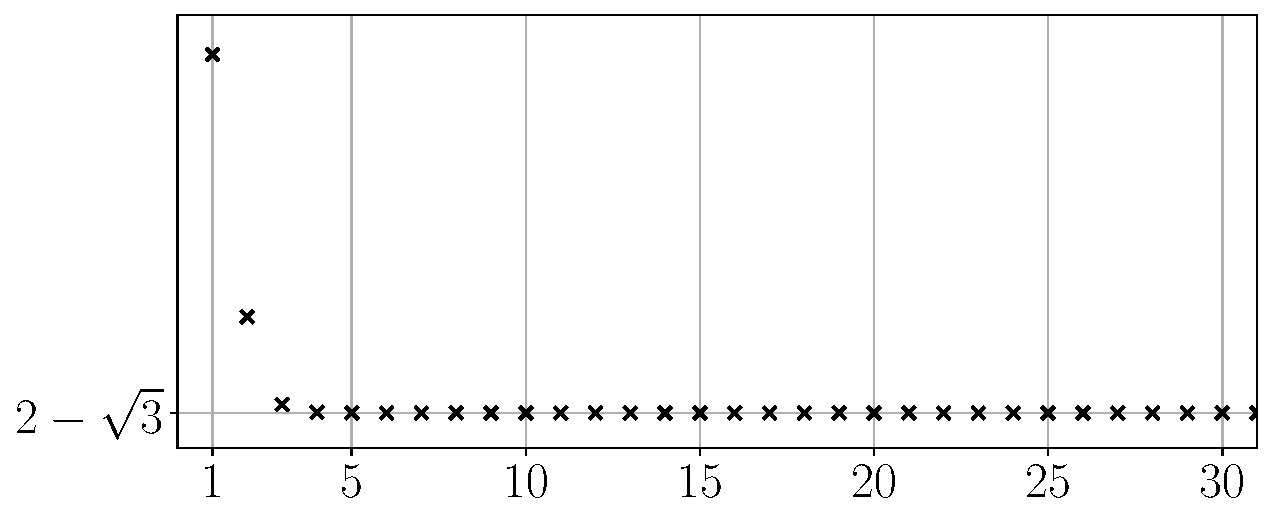
\includegraphics[width=0.8\textwidth]{UA_Figures/UA_ex2_4_1_fig.pdf}
        \caption{\( x_n \) for \( 1 \leq n \leq 30 \)}
        \label{fig:ex2.4.1}
    \end{figure}
\end{solution}

\begin{exercise}
\label{ex:2.4.2}
    \begin{enumerate}
        \item Consider the recursively defined sequence \( y_1 = 1 \),
        \[
            y_{n+1} = 3 - y_n,
        \]
        and set \( y = \lim y_n \). Because \( (y_n) \) and \( (y_{n+1}) \) have the same limit, taking the limit across the recursive equation gives \( y = 3 - y \). Solving for \( y \), we conclude \( \lim y_n = 3/2 \).

        What is wrong with this argument?

        \item This time set \( y_1 = 1 \) and \( y_{n+1} = 3 - \frac{1}{y_n} \). Can the strategy in (a) be applied to compute the limit of this sequence?
    \end{enumerate}
\end{exercise}

\begin{solution}
    \begin{enumerate}
        \item The problem is we have assumed that \( \lim y_n \) exists. Looking at the first few terms of the sequence \( y_1 = 1, y_2 = 2, y_3 = 1, y_4 = 2, \ldots \), we see that in fact the sequence oscillates and does not converge.

        \item The strategy works this time. Let \( P(n) \) be the statement that \( y_{n+1} \geq y_n \) and \( y_n \leq 3 \); we will use \href{https://en.wikipedia.org/wiki/Mathematical_induction#Complete_(strong)_induction}{strong induction} to show that \( P(n) \) holds for all \( n \in \N \). Since \( y_1 = 1 \) and \( y_2 = 2 \), we see that \( P(1) \) holds. Suppose that \( P(1), \ldots, P(n) \) all hold for some \( n \in \N \) and observe that
        \[
            y_{n+1} \geq y_n \geq 1 \implies \frac{1}{y_{n+1}} \leq \frac{1}{y_n} \implies 3 - \frac{1}{y_{n+1}} \geq 3 - \frac{1}{y_n},
        \]
        i.e., \( y_{n+2} \geq y_{n+1} \). Furthermore,
        \[
            1 \leq y_n \leq 3 \implies \frac{1}{3} \leq \frac{1}{y_n} \implies y_{n+1} = 3 - \frac{1}{y_n} \leq \frac{8}{3} < 3.
        \]
        Thus \( P(n + 1) \) holds. This completes the induction step and it follows that \( P(n) \) holds for all \( n \in \N \).

        We have now shown that \( (y_n) \) is bounded above and increasing, so by the Monotone Convergence Theorem (Theorem 2.4.2) we have \( \lim y_n = y \) for some \( y \in \R \). Given this, the following manipulations are valid:
        \[
            y_{n+1} = 3 - \frac{1}{y_n} \implies y = 3 - \frac{1}{y} \iff y^2 - 3y + 1 = 0.
        \]
        This quadratic equation has solutions \( \tfrac{3}{2} \pm \tfrac{1}{2} \sqrt{5} \). Since \( (y_n) \) is increasing and \( y_2 = 2 \), we must have \( y \geq 2 > \tfrac{3}{2} - \tfrac{1}{2} \sqrt{5} \) and so we may discard the solution \( y = \tfrac{3}{2} - \tfrac{1}{2} \sqrt{5} \) to conclude that \( \lim y_n = \tfrac{3}{2} + \tfrac{1}{2} \sqrt{5} \). See \Cref{fig:ex2.4.2} for a graph of the first thirty terms of \( (y_n) \).
    \end{enumerate}
    \begin{figure}[H]
        \centering
        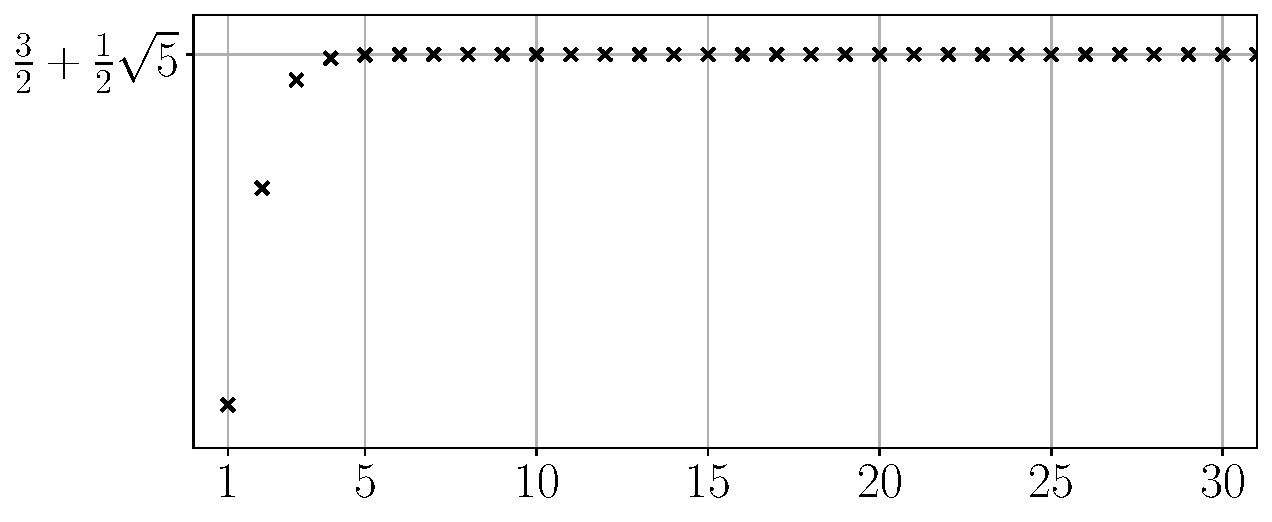
\includegraphics[width=0.8\textwidth]{UA_Figures/UA_ex2_4_2_fig.pdf}
        \caption{\( y_n \) for \( 1 \leq n \leq 30 \)}
        \label{fig:ex2.4.2}
    \end{figure}
\end{solution}

\begin{exercise}
\label{ex:2.4.3}
    \begin{enumerate}
        \item Show that
        \[
            \sqrt{2}, \sqrt{2 + \sqrt{2}}, \sqrt{2 + \sqrt{2 + \sqrt{2}}}, \ldots
        \]
        converges and find the limit.

        \item Does the sequence
        \[
            \sqrt{2}, \sqrt{2 \sqrt{2}}, \sqrt{2 \sqrt{2 \sqrt{2}}}, \ldots
        \]
        converge? If so, find the limit.
    \end{enumerate}
\end{exercise}

\begin{solution}
    \begin{enumerate}
        \item Let \( x_1 = \sqrt{2}, x_{n+1} = \sqrt{2 + x_n} \), and let \( P(n) \) be the statement that \( x_{n+1} \geq x_n \) and \( x_n \leq 2 \); we will use \href{https://en.wikipedia.org/wiki/Mathematical_induction#Complete_(strong)_induction}{strong induction} to show that \( P(n) \) holds for all \( n \in \N \). Since \( x_1 = \sqrt{2} \) and \( x_2 = \sqrt{2 + \sqrt{2}} \), we see that \( P(1) \) holds. Suppose that \( P(1), \ldots, P(n) \) all hold for some \( n \in \N \) and observe that
        \[
            x_{n+1} \geq x_n \geq \sqrt{2} \implies \sqrt{2 + x_{n+1}} \geq \sqrt{2 + x_n},
        \]
        i.e., \( x_{n+2} \geq x_{n+1} \). Furthermore,
        \[
            \sqrt{2} \leq x_n \leq 2 \implies \sqrt{2 + x_n} \leq \sqrt{4} = 2.  
        \]
        Thus \( P(n + 1) \) holds. This completes the induction step and it follows that \( P(n) \) holds for all \( n \in \N \).

        We have now shown that the sequence \( (x_n) \) is bounded above and increasing, so by the Monotone Convergence Theorem (Theorem 2.4.2) we have \( \lim x_n = x \) for some \( x \in \R \). We may now take the limit on both sides of the recursive equation:
        \[
            x_{n+1} = \sqrt{2 + x_n} \implies x = \sqrt{2 + x} \implies x^2 - x - 2 = 0 \iff (x - 2)(x + 1) = 0.
        \]
        So \( x = 2 \) or \( x = -1 \). Since the sequence is increasing and \( x_1 = \sqrt{2} \), we must have \( x \geq \sqrt{2} > -1 \) and thus \( \lim x_n = 2 \). See \Cref{fig:ex2.4.3_1} for a graph of the first thirty terms of the sequence \( (x_n) \).
        \begin{figure}[H]
            \centering
            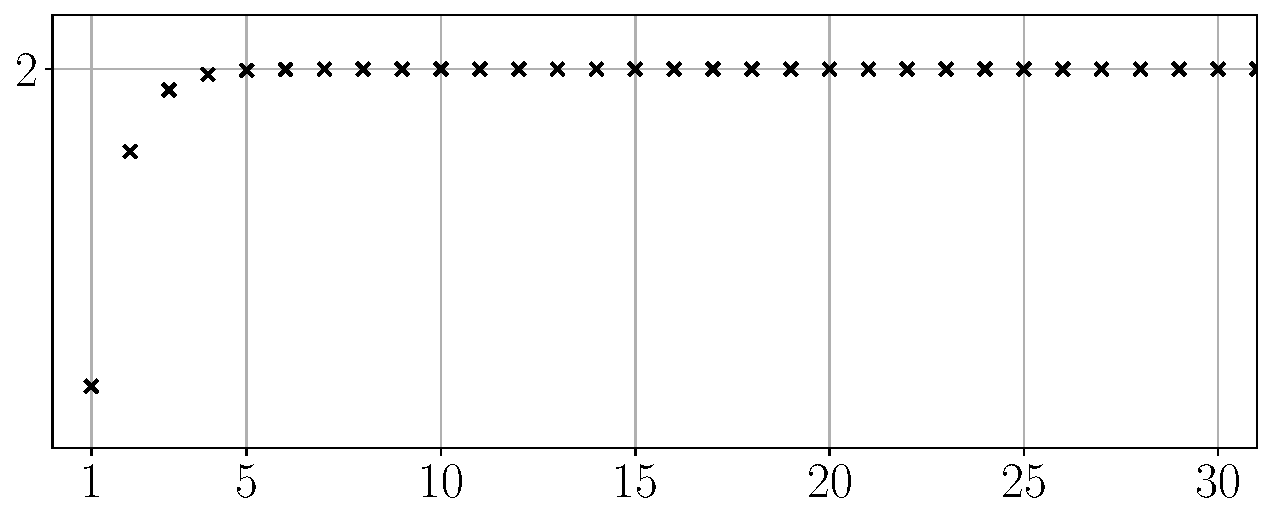
\includegraphics[width=0.8\textwidth]{UA_Figures/UA_ex2_4_3_fig_1.pdf}
            \caption{\( x_n \) for \( 1 \leq n \leq 30 \)}
            \label{fig:ex2.4.3_1}
        \end{figure}

        \item The sequence does converge. Let \( x_1 = \sqrt{2}, x_{n+1} = \sqrt{2 x_n}, \) and let \( P(n) \) be the statement that \( x_{n+1} \geq x_n \) and \( x_n \leq 2 \). We will use \href{https://en.wikipedia.org/wiki/Mathematical_induction#Complete_(strong)_induction}{strong induction} to show that \( P(n) \) holds for all \( n \in \N \). Since \( x_1 = \sqrt{2} \) and \( x_2 = \sqrt{2 \sqrt{2}} \), we see that \( P(1) \) holds. Suppose that \( P(1), \ldots, P(n) \) all hold for some \( n \in \N \) and observe that
        \[
            x_{n+1} \geq x_n \geq \sqrt{2} \implies \sqrt{2 x_{n+1}} \geq \sqrt{2 x_n},
        \]
        i.e., \( x_{n+2} \geq x_{n+1} \). Furthermore,
        \[
            \sqrt{2} \leq x_n \leq 2 \implies \sqrt{2 x_n} \leq \sqrt{4} = 2.
        \]
        Thus \( P(n + 1) \) holds. This completes the induction step and it follows that \( P(n) \) holds for all \( n \in \N \).
        
        We have shown that the sequence \( (x_n) \) is bounded above and increasing, so by the Monotone Convergence Theorem (Theorem 2.4.2) we have \( \lim x_n = x \) for some \( x \in \R \). We may now take the limit on both sides of the recursive equation:
        \[
            x_{n+1} = \sqrt{2 x_n} \implies x = \sqrt{2 x} \implies x^2 - 2x = 0 \iff x(x - 2) = 0.
        \]
        So \( x = 2 \) or \( x = 0 \). Since the sequence is increasing and \( x_1 = \sqrt{2} \), we must have \( x \geq \sqrt{2} > 0 \) and thus \( \lim x_n = 2 \). See \Cref{fig:ex2.4.3_2} for a graph of the first thirty terms of \( (x_n) \).
        \begin{figure}[H]
            \centering
            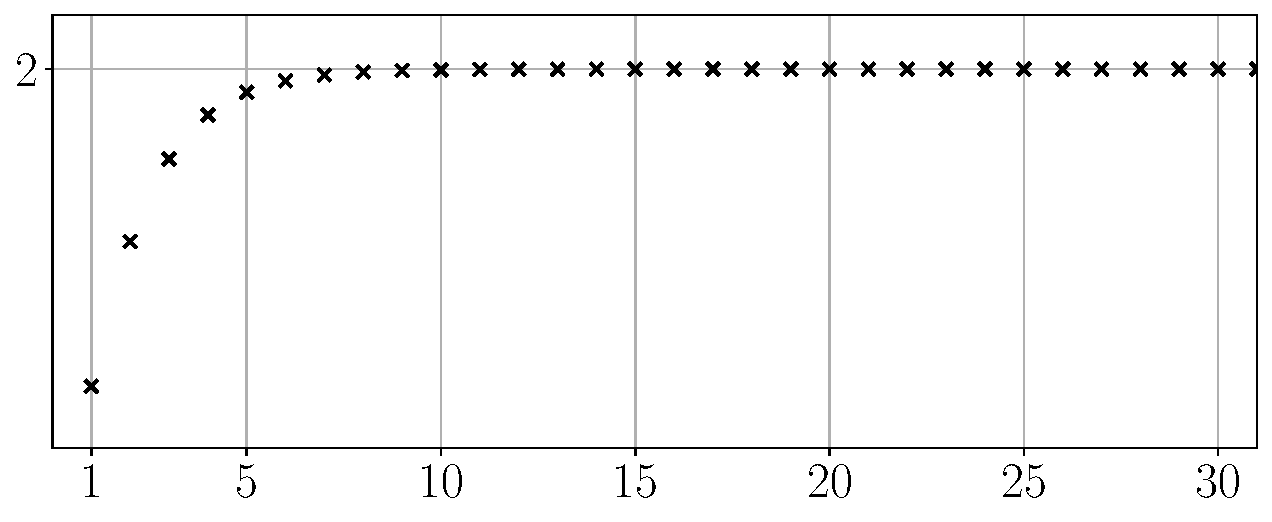
\includegraphics[width=0.8\textwidth]{UA_Figures/UA_ex2_4_3_fig_2.pdf}
            \caption{\( x_n \) for \( 1 \leq n \leq 30 \)}
            \label{fig:ex2.4.3_2}
        \end{figure}
    \end{enumerate}
\end{solution}

\begin{exercise}
\label{ex:2.4.4}
    \begin{enumerate}
        \item In Section 1.4 we used the Axiom of Completeness (AoC) to prove the Archimedean Property of \( \R \) (Theorem 1.4.2). Show that the Monotone Convergence Theorem can also be used to prove the Archimedean Property without making any use of AoC.

        \item Use the Monotone Convergence Theorem to supply a proof for the Nested Interval Property (Theorem 1.4.1) that doesn't make use of AoC.

        These two results suggest that we could have used the Monotone Convergence Theorem in place of AoC as our starting axiom for building a proper theory of the real numbers.
    \end{enumerate}
\end{exercise}

\begin{solution}
    \begin{enumerate}
        \item Assuming that any bounded monotone sequence converges, we want to prove part (i) of Theorem 1.4.2: for any \( x \in \R \), there exists an \( n \in \N \) satisfying \( n > x \). Part (ii) of Theorem 1.4.2 will then follow by taking \( x = \tfrac{1}{y} \) in part (i). Let \( x \) be given. Seeking a contradiction, suppose that \( n \leq x \) for each \( n \in \N \). Then the sequence \( (n) \) is bounded above and clearly monotone increasing, so by assumption this sequence converges, say \( \lim n = y \) for some \( y \in \R \). There then exists an \( N \in \N \) such that \( \abs{n - y} < \tfrac{1}{2} \) whenever \( n \geq N \). Observe that
        \[
            1 = \abs{N + 1 - y + y - N} \leq \abs{N + 1 - y} + \abs{N - y} < \frac{1}{2} + \frac{1}{2} = 1,
        \]
        i.e., \( 1 < 1 \), which is a contradiction. We may conclude that there exists some \( n \in \N \) such that \( n > x \).

        \item Assuming that any bounded monotone sequence converges, we want to prove that any sequence of nested intervals \( I_n = [a_n, b_n] \) has non-empty intersection. Consider the sequence \( (a_n) \) of left-hand endpoints. Because the intervals are nested, this is an increasing sequence which is bounded above by any right-hand endpoint, so by assumption this sequence converges, say \( \lim a_n = x \) for some \( x \in \R \). For any \( n \in \N \) we have \( a_n \leq a_m \leq b_m \leq b_n \) for all \( m \geq n \). The Order Limit Theorem (Theorem 2.3.4) then implies that \( x = \lim_{m \to \infty} a_m \leq b_n \) and \( a_n \leq \lim_{m \to \infty} a_m = x \); it follows that \( a_n \leq x \leq b_n \) for all \( n \in \N \), i.e., \( x \in \bigcap_{n=1}^{\infty} I_n \).
        \begin{center}
            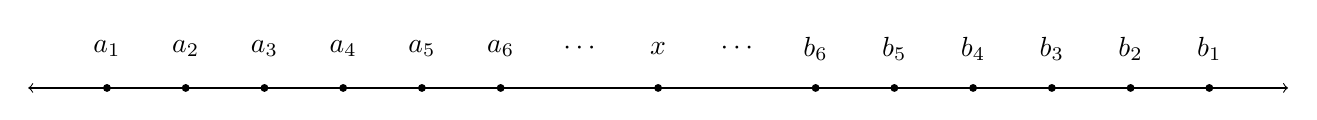
\begin{tikzpicture}
                \draw[<->] (-8, 0) -- (8, 0);
                \foreach [evaluate=\i as \x using -1 * \i] \i in {2,...,7}
                {
                    \fill (\i, 0) circle (0.05);
                    \fill (\x, 0) circle (0.05);
                }
                \foreach [evaluate=\i as \x using -8 + \i] \i in {1,...,6}
                {
                    \node at (\x, 0.5) {\( a_{\i} \)};
                }
                \foreach [evaluate=\i as \x using 8 - \i] \i in {1,...,6}
                {
                    \node at (\x, 0.5) {\( b_{\i} \)};
                }
                \node at (-1, 0.5) {\( \cdots \)};
                \node at (1, 0.5) {\( \cdots \)};
                \fill (0, 0) circle (0.05);
                \node at (0, 0.5) {\( x \)};
            \end{tikzpicture}
        \end{center}
    \end{enumerate}
\end{solution}

\begin{exercise}[Calculating Square Roots]
\label{ex:2.4.5}
    Let \( x_1 = 2 \), and define
    \[
        x_{n+1} = \frac{1}{2} \paren{ x_n + \frac{2}{x_n} }.
    \]
    \begin{enumerate}
        \item Show that \( x_n^2 \) is always greater than or equal to 2, and then use this to prove that \( x_n - x_{n+1} \geq 0 \). Conclude that \( \lim x_n = \sqrt{2} \).

        \item Modify the sequence \( (x_n) \) so that it converges to \( \sqrt{c} \).
    \end{enumerate}
\end{exercise}

\begin{solution}
    \begin{enumerate}
        \item Let \( P(n) \) be the statement that \( x_n \geq \sqrt{2} \). We will use induction to show that \( P(n) \) holds for all \( n \in \N \). The truth of \( P(1) \) is clear, so suppose that \( P(n) \) holds for some \( n \in \N \). Observe that
        \[
            \paren{ x_n - \sqrt{2} }^2 = x_n^2 - 2 \sqrt{2} x_n + 2 \geq 0.
        \]
        Our induction hypothesis guarantees that \( x_n \geq \sqrt{2} > 0 \) and so we may divide by \( x_n \) to obtain the inequality
        \[
            x_n - 2 \sqrt{2} + \frac{2}{x_n} \geq 0 \iff \frac{1}{2} \paren{ x_n + \frac{2}{x_n} } \geq \sqrt{2},
        \]
        i.e., \( x_{n+1} \geq \sqrt{2} \). This completes the induction step and thus \( P(n) \) holds for all \( n \in \N \); in particular, we have \( x_n^2 \geq 2 \) for each \( n \in \N \). Given this, for any \( n \in \N \) we have
        \begin{multline*}
            x_n^2 - 2 \geq 0 \iff x_n - \frac{2}{x_n} \geq 0 \iff \frac{x_n}{2} - \frac{1}{x_n} \geq 0 \\[2mm]
            \iff x_n - \frac{1}{2} \paren{ x_n + \frac{2}{x_n} } \geq 0 \iff x_n - x_{n+1} \geq 0.
        \end{multline*}
        It follows that the sequence \( (x_n) \) satisfies \( x_{n+1} \leq x_n \) for all \( n \in \N \).

        We have now shown that the sequence \( (x_n) \) is decreasing and bounded below. The Monotone Convergence Theorem (Theorem 2.4.2) then implies that \( \lim x_n = x \) for some \( x \in \R \). Since \( x_n \geq \sqrt{2} \) for all \( n \in \N \), the Order Limit Theorem (Theorem 2.3.4) implies that \( x \geq \sqrt{2} > 0 \) and so we can use the Algebraic Limit Theorem (Theorem 2.3.3) to take the limit across the recursive equation:
        \[
            x_{n+1} = \frac{1}{2} \paren{ x_n + \frac{2}{x_n} } \implies x = \frac{1}{2} \paren{ x + \frac{2}{x} } \implies x^2 = 2.
        \]
        Since \( x \geq \sqrt{2} \), we may conclude that \( x = \sqrt{2} \). See \Cref{fig:ex2.4.5} for a graph of the first thirty terms of the sequence \( (x_n) \).
        \begin{figure}[H]
            \centering
            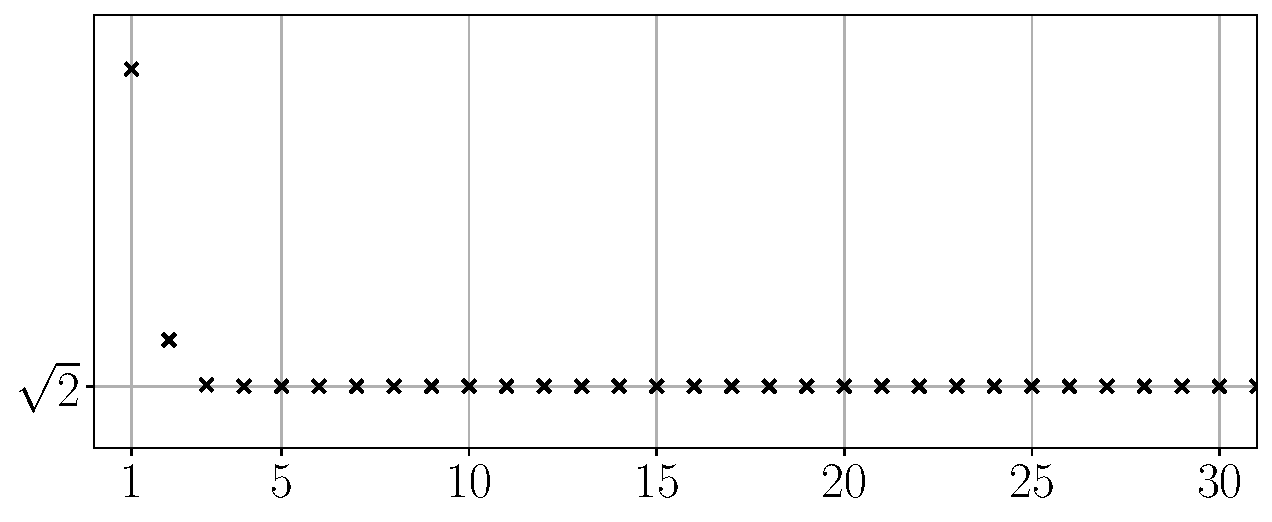
\includegraphics[width=0.8\textwidth]{UA_Figures/UA_ex2_4_5_fig.pdf}
            \caption{\( x_n \) for \( 1 \leq n \leq 30 \)}
            \label{fig:ex2.4.5}
        \end{figure}

        \item For \( c \geq 0 \), let \( x_1 = 1 + c \) and define
        \[
            x_{n+1} = \frac{1}{2} \paren{ x_n + \frac{c}{x_n} }.
        \]
        Repeating the argument given in part (a), replacing 2 with \( c \) where appropriate, shows that \( \lim x_n = \sqrt{c} \). For the base case of the induction argument, note that
        \[
            x_1 = 1 + c > 1 \implies x_1 = 1 + c > \sqrt{1 + c} > \sqrt{c}.
        \]
    \end{enumerate}
\end{solution}

\begin{exercise}[Arithmetic-Geometric Mean]
\label{ex:2.4.6}
    \begin{enumerate}
        \item Explain why \( \sqrt{xy} \leq (x + y)/2 \) for any two positive real numbers \( x \) and \( y \). (The geometric mean is always less than the arithmetic mean.)

        \item Now let \( 0 \leq x_1 \leq y_1 \) and define
        \[
            x_{n+1} = \sqrt{x_n y_n} \hspaceand[8mm] y_{n+1} = \frac{x_n + y_n}{2}.
        \]
        Show \( \lim x_n \) and \( \lim y_n \) both exist and are equal.
    \end{enumerate}
\end{exercise}

\begin{solution}
    \begin{enumerate}
        \item Observe that
        \[
            0 \leq (x - y)^2 \iff 0 \leq x^2 - 2xy + y^2 \iff 4xy \leq x^2 + 2xy + y^2 \iff 4xy \leq (x + y)^2.
        \]
        Since \( x \) and \( y \) are both positive, this implies that \( \sqrt{xy} \leq \tfrac{x + y}{2} \).

        \item By part (a), we have \( x_n \leq y_n \) for all \( n \in \N \). It follows that
        \[
            y_{n+1} = \frac{x_n + y_n}{2} \leq \frac{y_n + y_n}{2} = y_n \hspaceand[8mm] x_{n+1} = \sqrt{x_n y_n} \geq \sqrt{x_n^2} = x_n.
        \]
        Thus \( (x_n) \) is increasing and \( (y_n) \) is decreasing. Furthermore, \( (y_n) \) is bounded below: for any \( n \in \N \), we have
        \[
            y_n \geq x_n \geq \cdots \geq x_1.
        \]
        It follows from the Monotone Convergence Theorem (Theorem 2.4.2) that \( \lim y_n = y \) for some \( y \in \R \). The Algebraic Limit Theorem (Theorem 2.3.3) then gives
        \[
            x_n = 2 y_{n+1} - y_n \implies \lim x_n = 2 \lim y_{n+1} - \lim y_n = 2 y - y = y.
        \]
    \end{enumerate}
\end{solution}

\begin{exercise}[Limit Superior]
\label{ex:2.4.7}
    Let \( (a_n) \) be a bounded sequence.
    \begin{enumerate}
        \item Prove that the sequence defined by \( y_n = \sup \{ a_k : k \geq n \} \) converges.

        \item The \textit{limit superior} of \( (a_n) \), or \( \limsup a_n \), is defined by
        \[
            \limsup a_n = \lim y_n,
        \]
        where \( y_n \) is the sequence from part (a) of this exercise. Provide a reasonable definition for \( \liminf a_n \) and briefly explain why it always exists for any bounded sequence.

        \item Prove that \( \liminf a_n \leq \limsup a_n \) for every bounded sequence, and give an example of a sequence for which the inequality is strict.

        \item Show that \( \liminf a_n = \limsup a_n \) if and only if \( \lim a_n \) exists. In this case, all three share the same value.
    \end{enumerate}
\end{exercise}

\begin{solution}
    \begin{enumerate}
        \item Suppose \( M > 0 \) is the bound for \( (a_n) \), i.e., \( \abs{a_n} \leq M \) for all \( n \in \N \). It follows that \( y_n \geq a_n \geq -M \) for any \( n \in \N \), so that the sequence \( (y_n) \) is bounded below. Furthermore, for any \( n \in \N \) we have
        \begin{multline*}
            \{ a_k : k \geq n + 1 \} \subseteq \{ a_k : k \geq n \} \implies \sup \{ a_k : k \geq n + 1 \} \leq \sup \{ a_k : k \geq n \} \\[2mm]
            \iff y_{n+1} \leq y_n,
        \end{multline*}
        i.e., the sequence \( (y_n) \) is decreasing. We may now invoke the Monotone Convergence Theorem (Theorem 2.4.2) to conclude that \( (y_n) \) converges.

        \item Let \( z_n = \inf \{ a_k : k \geq n \} \). Similarly to part (a), we can show that this sequence is bounded above, increasing, and hence convergent. We then define the limit inferior as \( \liminf a_n = \lim z_n \).

        \item The infimum of a bounded set is always less than or equal to the supremum of that set, so we have \( z_n \leq y_n \) for each \( n \in \N \). The Order Limit Theorem (Theorem 2.3.4) then implies that \( \lim z_n \leq \lim y_n \), i.e., \( \liminf a_n \leq \limsup a_n \).

        For an example of a bounded sequence where this inequality is strict, consider the sequence \( a_n = (-1)^n \). For this sequence we have \( y_n = (1, 1, 1, \ldots) \) and \( z_n = (-1, -1, -1, \ldots ) \), so that \( \liminf a_n = -1 < 1 = \limsup a_n \).

        \item Suppose \( \liminf a_n = \limsup a_n \). Since \( z_n \leq a_n \leq y_n \) for all \( n \in \N \), the Squeeze Theorem (\Cref{ex:2.3.3}) implies that \( (a_n) \) converges and that \( \liminf a_n = \limsup a_n = \lim a_n \).
        
        Now suppose that \( \lim a_n = a \) for some \( a \in \R \) and let \( \epsilon > 0 \) be given. Since \( a_n \to a \), there is an \( N \in \N \) such that
        \[
            n \geq N \implies a - \frac{\epsilon}{2} < a_n < a + \frac{\epsilon}{2}.
        \]
        This implies that \( a - \tfrac{\epsilon}{2} \) is a lower bound for \( \{ a_k : k \geq N \} \) and that \( a + \tfrac{\epsilon}{2} \) is an upper bound for \( \{ a_k : k \geq N \} \). It follows that \( a - \tfrac{\epsilon}{2} \leq z_N \leq a_N \leq y_N \leq a + \tfrac{\epsilon}{2} \). Since \( (z_n) \) is increasing and \( (y_n) \) is decreasing, we then have
        \[
            n \geq N \implies a - \epsilon < a - \frac{\epsilon}{2} \leq z_N \leq z_n \leq a_n \leq y_n \leq y_N \leq a + \frac{\epsilon}{2} < a + \epsilon,
        \]
        i.e., \( \abs{z_n - a} < \epsilon \) and \( \abs{y_n - a} < \epsilon \) for all \( n \geq N \). It follows that \( \liminf a_n = \limsup a_n = \lim a_n = a \).
    \end{enumerate}
\end{solution}

\begin{exercise}
\label{ex:2.4.8}
    For each series, find an explicit formula for the sequence of partial sums and determine if the series converges.
    \[
        \text{(a) } \sum_{n=1}^{\infty} \frac{1}{2^n} \qquad \text{(b) } \sum_{n=1}^{\infty} \frac{1}{n(n+1)} \qquad \text{(c) } \sum_{n=1}^{\infty} \log \paren{ \frac{n+1}{n} }
    \]
    (In (c), \( \log(x) \) refers to the natural logarithm function from calculus.)
\end{exercise}

\begin{solution}
    For each series, let \( (s_m) \) be its sequence of partial sums; see \Cref{fig:ex2.4.8} for graphs of the first thirty terms of these partial sum sequences.
    \begin{enumerate}
        \item Here we have
        \begin{align*}
            s_m &= \frac{1}{2} + \frac{1}{2^2} + \cdots + \frac{1}{2^{m-1}} + \frac{1}{2^m} \\[2mm]
            \implies 2 s_m &= 1 + \frac{1}{2} + \cdots + \frac{1}{2^m} + \frac{1}{2^{m+1}} \\[2mm]
            \implies 2 s_m &= \frac{1 - 2^{-(m+2)}}{1 - \tfrac{1}{2}} \\[2mm]
            \implies s_m &= 1 - \frac{1}{2^{m+2}},
        \end{align*}
        where we have used the formula \( (1 - x)(1 + x + x^2 + \cdots + x^n) = 1 - x^{n+1} \). It follows that \( \lim s_m = 1 \).

        \item For this series,
        \begin{multline*}
            s_m = \sum_{n=1}^m \frac{1}{n(n+1)} = \sum_{n=1}^m \paren{ \frac{1}{n} - \frac{1}{n+1} } \\[2mm]
            = \paren{ 1 - \frac{1}{2} } + \paren{ \frac{1}{2} - \frac{1}{3} } + \cdots + \paren{ \frac{1}{m} - \frac{1}{m+1} } = 1 - \frac{1}{m+1}.
        \end{multline*}
        It follows that \( \lim s_m = 1 \).

        \item We have
        \begin{align*}
            s_m &= \sum_{n=1}^m \log \paren{ \frac{n+1}{n} } \\[2mm]
            &= \sum_{n=1}^m \paren{ \log(n+1) - \log(n) } \\[2mm]
            &= \paren{ \log(2) - \log(1) } + \paren{ \log(3) - \log(2) } + \cdots + \paren{ \log(m+1) - \log(m) } \\[2mm]
            &= \log(m+1).
        \end{align*}
        So \( s_m = \log(m+1) \), which is unbounded and hence not convergent.
    \end{enumerate}
    \begin{figure}[H]
        \centering
        \begin{subfigure}{0.75\textwidth}
            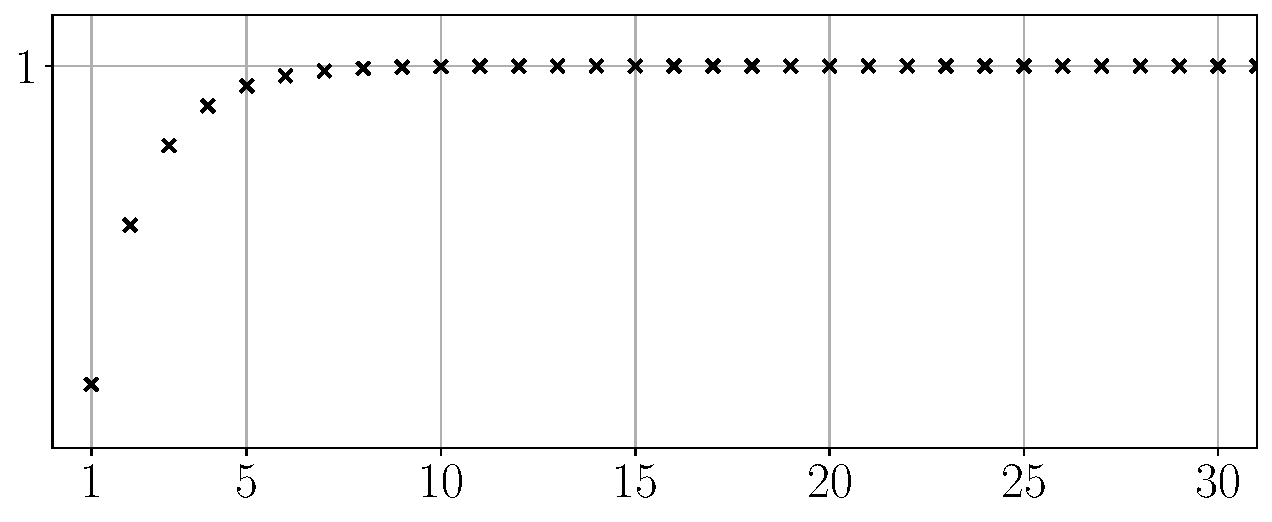
\includegraphics[width=\textwidth]{UA_Figures/UA_ex2_4_8_fig_a.pdf}
            \caption{\( \sum_{n=1}^m \tfrac{1}{2^n} \) for \( 1 \leq m \leq 30 \)}
        \end{subfigure} \\
        \begin{subfigure}{0.75\textwidth}
            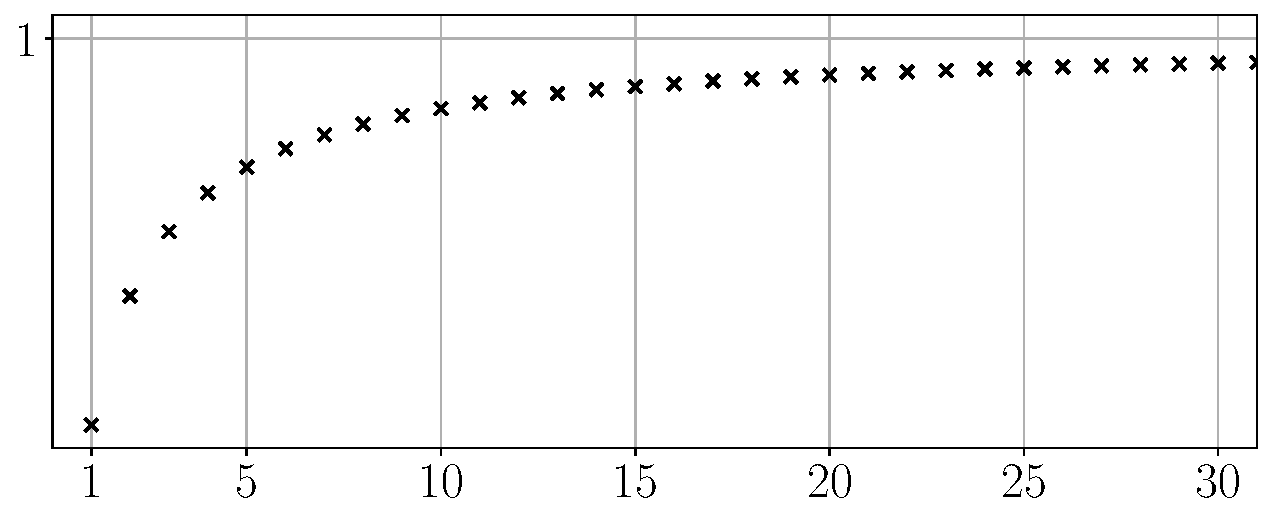
\includegraphics[width=\textwidth]{UA_Figures/UA_ex2_4_8_fig_b.pdf}
            \caption{\( \sum_{n=1}^m \tfrac{1}{n(n+1)} \) for \( 1 \leq m \leq 30 \)}
        \end{subfigure} \\
        \begin{subfigure}{0.75\textwidth}
            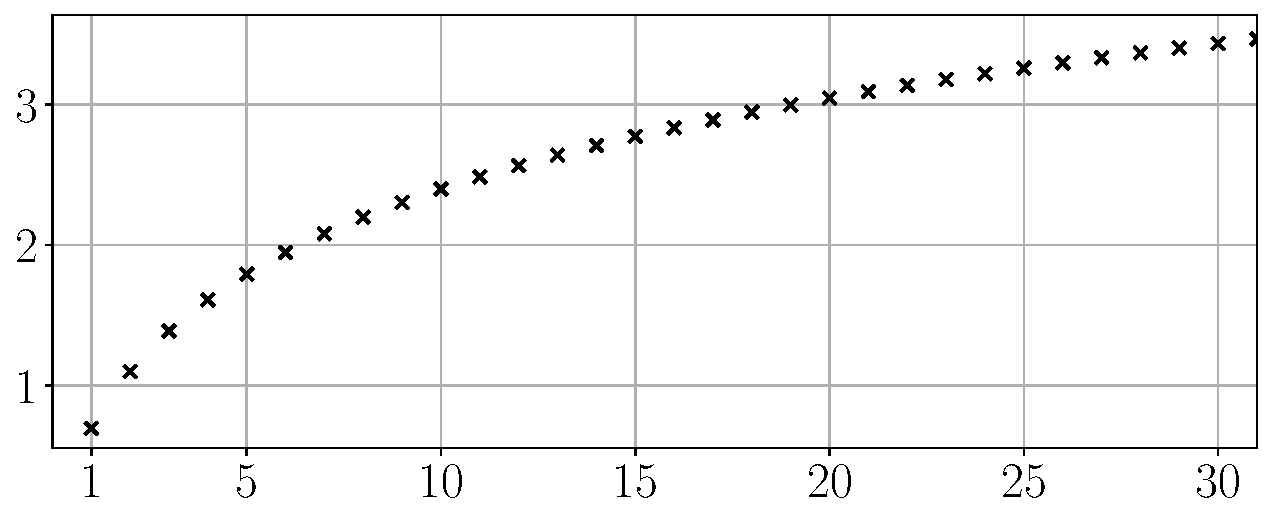
\includegraphics[width=\textwidth]{UA_Figures/UA_ex2_4_8_fig_c.pdf}
            \caption{\( \sum_{n=1}^m \log \paren{ \tfrac{n+1}{n} } \) for \( 1 \leq m \leq 30 \)}
        \end{subfigure}
        \caption{\Cref{ex:2.4.8} partial sums for \( 1 \leq m \leq 30 \)}
        \label{fig:ex2.4.8}
    \end{figure}
\end{solution}

\begin{exercise}
\label{ex:2.4.9}
    Complete the proof of Theorem 2.4.6 by showing that if the series \( \sum_{n=0}^{\infty} 2^n b_{2^n} \) diverges, then so does \( \sum_{n=1}^{\infty} b_n \). Example 2.4.5 may be a useful reference.
\end{exercise}

\begin{solution}
    Define the sequences of partial sums
    \[
        s_m = b_1 + b_2 + \cdots + b_m \hspaceand[8mm] t_m = b_1 + 2 b_2 + \cdots + 2^m b_{2^m}.
    \]
    We will use induction to show that \( t_m \leq 2 s_{2^m} \) for each \( m \in \N \). For the base case \( m = 1 \) we have
    \[
        t_1 = b_1 + 2 b_2 \leq 2 b_1 + 2 b_2 = 2 s_2,
    \]
    where we have used that \( b_1 \) is non-negative. Suppose that the inequality holds for some \( m \in \N \). Because the sequence \( (b_n) \) is decreasing, we have \( b_{2^{m+1}} \leq b_{2^m + j} \) for each \( 1 \leq j \leq 2^m \). It follows that \( 2^m b_{2^{m+1}} \leq \sum_{j=1}^{2^m} b_{2^m + j} \). Combining this inequality with our induction hypothesis, we see that
    \[
        t_{m+1} = t^m + 2^{m+1} b_{2^{m+1}} \leq 2 s_{2^m} + 2 \sum_{j=1}^{2^m} b_{2^m + j} = 2 s_{2^{m+1}}.
    \]
    This completes the induction step.

    Since each \( b_n \) is non-negative, both sequences of partial sums \( (s_m) \) and \( (t_m) \) are increasing. It follows from the Monotone Convergence Theorem (Theorem 2.4.2) that the convergence of each series is equivalent to the boundedness of the respective sequence of partial sums. Given this, we want to show that if \( (t_m) \) is unbounded, then so is \( (s_m) \); this follows immediately from the inequality \( t_m \leq 2 s_{2^m} \).
\end{solution}

\begin{exercise}[Infinite Products]
\label{ex:2.4.10}
    A close relative of infinite series is the \textit{infinite product}
    \[
        \prod_{n=1}^{\infty} b_n = b_1 b_2 b_3 \cdots
    \]
    which is understood in terms of its sequence of \textit{partial products}
    \[
        p_m = \prod_{n=1}^m b_n = b_1 b_2 b_3 \cdots b_m.
    \]
    Consider the special class of infinite products of the form
    \[
        \prod_{n=1}^{\infty} (1 + a_n) = (1 + a_1)(1 + a_2)(1 + a_3) \cdots, \quad \text{where } a_n \geq 0.
    \]
    \begin{enumerate}
        \item Find an explicit formula for the sequence of partial products in the case where \( a_n = 1/n \) and decide whether the sequence converges. Write out the first few terms in the sequence of partial products in the case where \( a_n = 1/n^2 \) and make a conjecture about the convergence of this sequence.

        \item Show, in general, that the sequence of partial products converges if and only if \( \sum_{n=1}^{\infty} a_n \) converges. (The inequality \( 1 + x \leq 3^x \) for positive \( x \) will be useful in one direction.)
    \end{enumerate}
\end{exercise}

\begin{solution}
    \begin{enumerate}
        \item For \( a_n = \tfrac{1}{n} \), observe that
        \begin{multline*}
            p_m = \prod_{n=1}^m \paren{ 1 + \frac{1}{n} } = \prod_{n=1}^m \paren{ \frac{n + 1}{n} } = 2 \cdot \frac{3}{2} \cdot \frac{4}{3} \cdots \frac{m}{m - 1} \cdot \frac{m + 1}{m} \\[2mm]
            = \frac{2}{2} \cdot \frac{3}{3} \cdot \frac{4}{4} \cdots \frac{m}{m} \cdot (m + 1) = m + 1.
        \end{multline*}
        It follows that \( (p_m) \) does not converge.
        
        For \( a_n = \tfrac{1}{n^2} \), the first few partial products are
        \begin{align*}
            p_1 &= 2, \\
            p_2 &= 2(1 + 1/4) = 5/2 = 2.5, \\
            p_3 &= (5/2)(1 + 1/9) = 25/9 \approx 2.778, \\
            p_4  &= (25/9)(1 + 1/16) = 425/144 \approx 2.951.
        \end{align*}
        It looks like the partial products could be bounded; we conjecture that this infinite product converges. Indeed, part (b) proves our conjecture, since \( \sum_{n=1}^{\infty} \tfrac{1}{n^2} \) is a convergent series; the \href{https://en.wikipedia.org/wiki/Weierstrass_factorization_theorem}{Weierstrass factorization theorem} can be used to show that
        \[
            \prod_{n=1}^{\infty} \paren{ 1 + \frac{1}{n^2} } = \frac{\sinh (\pi)}{\pi}.
        \]
        See \Cref{fig:ex2.4.10} for a graph of the first thirty terms of the partial product sequence.
        \begin{figure}[H]
            \centering
            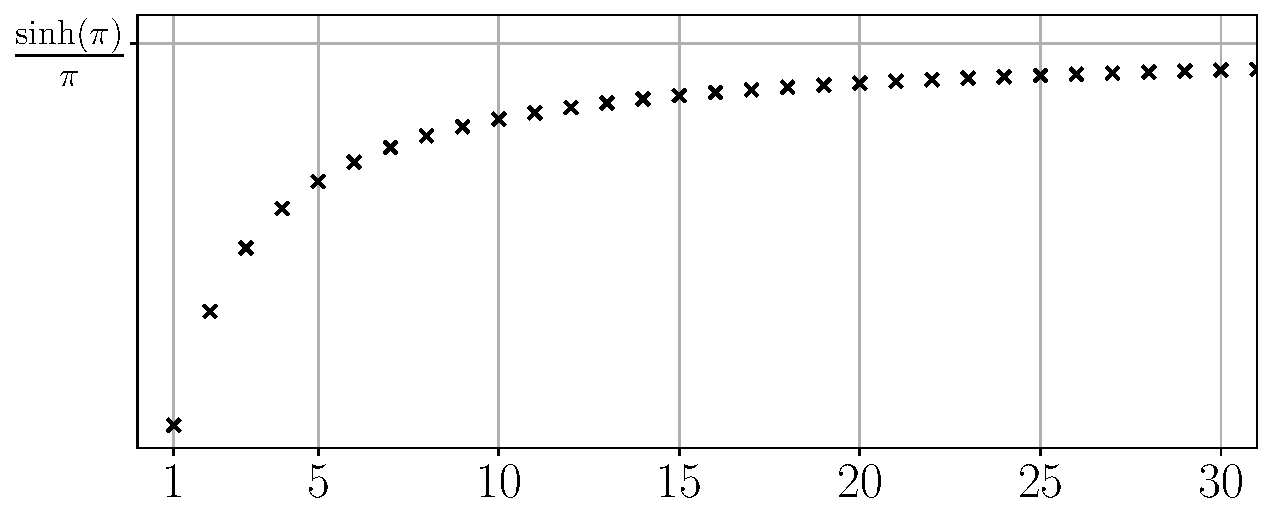
\includegraphics[width=0.8\textwidth]{UA_Figures/UA_ex2_4_10_fig.pdf}
            \caption{\( \prod_{n=1}^m \left( 1 + \frac{1}{n^2} \right) \) for \( 1 \leq m \leq 30 \)}
            \label{fig:ex2.4.10}
        \end{figure}

        \item Let
        \[
            s_m = \sum_{n=1}^m a_n \hspaceand p_m = \prod_{n=1}^m (1 + a_n).
        \]
        Since \( a_n \geq 0 \) for all \( n \in \N \), the sequence of partial sums and the sequence of partial products are both non-negative and increasing. It follows from the Monotone Convergence Theorem (Theorem 2.4.2) that the convergence of each sequence is equivalent to the boundedness of that sequence. By multiplying out the terms in the partial product \( p_m \), we would obtain the sum \( s_m \) and some other non-negative terms; it follows that \( s_m \leq p_m \). The hint gives us
        \[
            p_m = \prod_{n=1}^m (1 + a_n) \leq \prod_{n=1}^m 3^{a_n} = 3^{\sum_{n=1}^m a_n} = 3^{s_m}.
        \]
        So we have the inequalities \( s_m \leq p_m \leq 3^{s_m} \). It is then clear that \( (s_m) \) is bounded if \( (p_m) \) is bounded, and furthermore if \( (s_m) \) is bounded by some \( M > 0 \), then \( (p_m) \) is bounded by \( 3^M \). It follows that for this special case, \( \prod_{n=1}^{\infty} (1 + a_n) \) converges if and only if \( \sum_{n=1}^{\infty} a_n \) converges.
    \end{enumerate}
\end{solution}

\section{Subsequences and the Bolzano-Weierstrass Theorem}
\label{sec:2.5}

\begin{exercise}
\label{ex:2.5.1}
    Give an example of each of the following, or argue that such a request is impossible.
    \begin{enumerate}
        \item A sequence that has a subsequence that is bounded but contains no subsequence that converges.

        \item A sequence that does not contain 0 or 1 as a term but contains subsequences converging to each of these values.

        \item A sequence that contains subsequences converging to every point in the infinite set
        \[
            \{ 1, 1/2, 1/3, 1/4, 1/5, \ldots \}.
        \]

        \item A sequence that contains subsequences converging to every point in the infinite set
        \[
            \{ 1, 1/2, 1/3, 1/4, 1/5, \ldots \},
        \]
        and no subsequences converging to points outside of this set.
    \end{enumerate}
\end{exercise}

\begin{solution}
    \begin{enumerate}
        \item This is impossible. If a sequence \( (a_n) \) has a bounded subsequence \( \paren{ a_{n_k} } \), then by the Bolzano-Weierstrass Theorem (Theorem 2.5.5) there must be a convergent sub-subsequence \( \big( a_{n_{k_{\ell}}} \big) \); this is also a convergent subsequence of the original sequence \( (a_n) \).

        \item Consider the sequence
        \[
            \paren{ \frac{1}{2}, \frac{1}{2}, \frac{1}{4}, \frac{3}{4}, \frac{1}{6}, \frac{5}{6}, \ldots },
        \]
        i.e., the sequence \( (a_n) \) given by
        \[
            a_n = \begin{cases}
                \frac{1}{n+1} & \text{if } n \text{ is odd}, \\
                1 - \frac{1}{n} & \text{if } n \text{ is even}.
            \end{cases}
        \]
        This sequence does not contain 0 or 1 as a term, the subsequence \( (a_{2n - 1}) \) converges to 0, and the subsequence \( (a_{2n}) \) converges to 1.

        \item Consider the following infinite array:
        \begin{gather*}
            \arraycolsep=3mm\def\arraystretch{1.5}
            \begin{matrix}
                1 & \tfrac{1}{2} & \tfrac{1}{3} & \tfrac{1}{4} & \tfrac{1}{5} & \cdots \\
                1 & \tfrac{1}{2} & \tfrac{1}{3} & \tfrac{1}{4} & \tfrac{1}{5} & \cdots \\
                1 & \tfrac{1}{2} & \tfrac{1}{3} & \tfrac{1}{4} & \tfrac{1}{5} & \cdots \\
                1 & \tfrac{1}{2} & \tfrac{1}{3} & \tfrac{1}{4} & \tfrac{1}{5} & \cdots \\
                1 & \tfrac{1}{2} & \tfrac{1}{3} & \tfrac{1}{4} & \tfrac{1}{5} & \cdots \\
                \vdots & \vdots & \vdots & \vdots & \vdots & \ddots
            \end{matrix}
        \end{gather*}
        Let \( (a_n) \) be the sequence obtained by following the diagonals of this array, i.e.,
        \[
            (a_n) = \paren{ 1, 1, \tfrac{1}{2}, 1, \tfrac{1}{2}, \tfrac{1}{3}, 1, \tfrac{1}{2}, \tfrac{1}{3}, \tfrac{1}{4}, 1, \ldots }.
        \]
        The subsequence given by the \( n \)\ts{th} column is \( \paren{ \tfrac{1}{n}, \tfrac{1}{n}, \tfrac{1}{n}, \ldots } \), which converges to \( \tfrac{1}{n} \).

        \item This is impossible. Suppose that \( (a_n) \) is a sequence that contains subsequences converging to every point in the infinite set
        \[
            \set{ 1, \frac{1}{2}, \frac{1}{3}, \frac{1}{4}, \frac{1}{5}, \ldots }.
        \]
        We claim that \( (a_n) \) must have a subsequence converging to 0. We will construct this subsequence recursively as follows. Since there is a subsequence converging to 1, there must be some index \( n_1 \) such that
        \[
            \abs{a_{n_1} - 1} < 1 \iff 0 < a_{n_1} < 2.
        \]
        Since there is a subsequence converging to \( \tfrac{1}{2} \), there must be some index \( n_2 > n_1 \) such that
        \[
            \abs{a_{n_2} - \frac{1}{2}} < \frac{1}{2} \iff 0 < a_{n_2} < 1.
        \]
        We continue in this manner, obtaining a subsequence \( (a_{n_k}) \) satisfying \( 0 < a_{n_k} < \tfrac{2}{k} \). The Squeeze Theorem (\Cref{ex:2.3.3}) then implies that \( \lim_{k \to \infty} a_{n_k} = 0 \).
    \end{enumerate}
\end{solution}

\begin{exercise}
\label{ex:2.5.2}
    Decide whether the following propositions are true or false, providing a short justification for each conclusion.
    \begin{enumerate}
        \item If every proper subsequence of \( (x_n) \) converges, then \( (x_n) \) converges as well.

        \item If \( (x_n) \) contains a divergent subsequence, then \( (x_n) \) diverges.

        \item If \( (x_n) \) is bounded and diverges, then there exist two subsequences of \( (x_n) \) that converge to different limits.

        \item If \( (x_n) \) is monotone and contains a convergent subsequence, then \( (x_n) \) converges.
    \end{enumerate}
\end{exercise}

\begin{solution}
    \begin{enumerate}
        \item This is true. By assumption, the subsequence \( (x_2, x_3, x_4, \ldots) \) converges; it follows that \( (x_n) \) also converges to the same limit (see \Cref{ex:2.4.1} (b)).

        \item This is true. Consider the contrapositive statement: if \( (x_n) \) converges, then all subsequences of \( (x_n) \) converge. This is implied by Theorem 2.5.2.

        \item This is true. Consider the sequences
        \[
            y_n = \sup \{ x_m : m \geq n \} \hspaceand z_n = \inf \{ x_m : m \geq n \}.
        \]
        As shown in \Cref{ex:2.4.7}, these sequences both converge since \( (x_n) \) is bounded and their limits are denoted by
        \[
            \limsup x_n = \lim y_n \hspaceand \liminf x_n = \lim z_n.
        \]
        We claim that there are subsequences of \( (x_n) \) converging to \( \limsup x_n \) and \( \liminf x_n \). First, we will recursively construct a subsequence converging to \( \limsup x_n \). Let \( n_0 = 0 \). By Lemma 1.3.8, there exists an \( n_1 \geq 1 \) such that \( y_1 - 1 < x_{n_1} \leq y_1 \). There then exists an \( n_2 \geq n_1 + 1 \) such that \( y_{n_1 + 1} - \tfrac{1}{2} < x_{n_2} \leq y_{n_1 + 1} \). Continuing in this fashion, we obtain indices \( n_1 < \cdots < n_k < \cdots \) such that
        \[
            y_{n_{k-1} + 1} - \frac{1}{k} < x_{n_k} \leq y_{n_{k-1} + 1}
        \]
        for each \( k \in \N \). The subsequence \( (y_{n_{k-1} + 1}) \) converges to \( \limsup x_n \) (Theorem 2.5.2) and hence by the Squeeze Theorem (\Cref{ex:2.3.3}) the subsequence \( (x_{n_k}) \) converges to \( \limsup x_n \). Similarly, we can obtain another subsequence converging to \( \liminf x_n \). As we showed in \Cref{ex:2.4.7}, the fact that \( (x_n) \) diverges implies that \( \liminf x_n < \limsup x_n \) and so we have found two subsequences of \( (x_n) \) that converge to different limits.

        \item This is true. Suppose that \( (x_n) \) is decreasing; the case where \( (x_n) \) is increasing is handled similarly. By assumption, there is a subsequence \( (x_{n_k}) \), which must also be decreasing, converging to some \( x \in \R \). By the Monotone Convergence Theorem (Theorem 2.4.2) and the uniqueness of limits (Theorem 2.2.7/\Cref{ex:2.2.6}), we have
        \[
            \lim_{k \to \infty} x_{n_k} = x = \inf \{ x_{n_k} : k \in \N \}.
        \]
        Let \( \epsilon > 0 \) be given. Since \( x_{n_k} \to x \), there is a \( K \in \N \) such that \( \abs{x_{n_K} - x} < \epsilon \). Suppose that \( n \in \N \) is such that \( n \geq n_K \). Because \( (x_{n_k}) \) is a subsequence, there exists some \( k \in \N \) such that \( n_k \geq n \). Since \( (x_n) \) is decreasing, we then have
        \[
            x \leq x_{n_k} \leq x_n \leq x_{n_K} < x + \epsilon \implies \abs{x_n - x} < \epsilon.
        \]
        Thus \( \lim_{n \to \infty} x_n = x \).
    \end{enumerate}
\end{solution}

\begin{exercise}
\label{ex:2.5.3}
    \begin{enumerate}
        \item Prove that if an infinite series converges, then the associative property holds. Assume \( a_1 + a_2 + a_3 + a_4 + a_5 + \cdots \) converges to a limit \( L \) (i.e., the sequence of partial sums \( (s_n) \to L \)). Show that any regrouping of the terms
        \[
            (a_1 + a_2 + \cdots + a_{n_1}) + (a_{n_1 + 1} + \cdots + a_{n_2}) + (a_{n_2 + 1} + \cdots + a_{n_3}) + \cdots
        \]
        leads to a series that also converges to \( L \).

        \item Compare this result to the example discussed at the end of Section 2.1 where infinite addition was shown not to be associative. Why doesn't our proof in (a) apply to this example?
    \end{enumerate}
\end{exercise}

\begin{solution}
    \begin{enumerate}
        \item We have indices \( n_1 < \cdots < n_k < \cdots \) and we want to show that \( \sum_{k=1}^{\infty} b_k = L \), where \( b_1 = a_1 + \cdots + a_{n_1} = s_{n_1} \) and
        \[
            b_k = a_{n_{k-1} + 1} + \cdots + a_{n_k} = s_{n_k} - s_{n_{k-1}}
        \]
        for \( k \geq 2 \). Observe that for \( m \geq 2 \), the partial sums are
        \[
            t_m = \sum_{k=1}^m b_k = s_{n_1} + \sum_{k=2}^m (s_{n_k} - s_{n_{k-1}}) = s_{n_1} + (s_{n_2} - s_{n_1}) + \cdots + (s_{n_m} - s_{n_{m-1}}) = s_{n_m}.
        \]
        It follows from Theorem 2.5.2 that \( \sum_{k=1}^{\infty} b_k = \lim_{m \to \infty} t_m = \lim_{m \to \infty} s_{n_m} = L \).

        \item Our proof does not apply to the series \( \sum_{n=1}^{\infty} (-1)^n \) since this series does not converge: the sequence of partial sums is \( (-1, 0, -1, 0, \ldots) \).
    \end{enumerate}
\end{solution}

\begin{exercise}
\label{ex:2.5.4}
    The Bolzano-Weierstrass Theorem is extremely important, and so is the strategy employed in the proof. To gain some more experience with this technique, assume the Nested Interval Property is true and use it to provide a proof of the Axiom of Completeness. To prevent the argument from being circular, assume also that \( (1/2^n) \to 0 \). (Why precisely is this last assumption needed to avoid circularity?)
\end{exercise}

\begin{solution}
    Let \( E \subseteq \R \) be non-empty and bounded above by some \( b_1 \in \R \); we will show that \( \sup E \) exists. If \( E \) has a maximum \( x \), then \( \sup E = x \) and we are done. Otherwise, we shall use a recursive argument to construct a sequence \( (I_n)_{n=1}^{\infty} \) of nested intervals. Pick some \( a_1 \in E \); it must be the case that \( a_1 \) is not an upper bound of \( E \) since \( E \) has no maximum. Let \( I_1 = [a_1, b_1] \) and note that:
    \begin{itemize}
        \item \( a_1 \) is not an upper bound of \( E \);

        \item \( b_1 \) is an upper bound of \( E \);

        \item \( \abs{I_1} = 2^0 (b_1 - a_1) \).
    \end{itemize}
    Suppose that after \( N \) steps we have chosen intervals \( I_n = [a_n, b_n], 1 \leq n \leq N \), such that
    \begin{itemize}
        \item \( a_1 \leq \cdots \leq a_N \) are not upper bounds of \( E \);

        \item \( b_N \leq \cdots \leq b_1 \) are upper bounds of \( E \);

        \item \( \abs{I_n} = 2^{-(n-1)}(b_1 - a_1) \) for \( 1 \leq n \leq N \).
    \end{itemize}
    Let \( m = \tfrac{a_N + b_N}{2} \), the midpoint of the interval \( I_N \). If \( m \) is not an upper bound of \( E \), let
    \[
        a_{N+1} = m, \quad b_{N+1} = b_N, \hspaceand I_{N+1} = [a_{N+1}, b_{N+1}].
    \]
    If \( m \) is an upper bound of \( E \), let
    \[
        a_{N+1} = a_N, \quad b_{N+1} = m, \hspaceand I_{N+1} = [a_{N+1}, b_{N+1}].
    \]
    In either case, we have chosen intervals \( I_n = [a_n, b_n], 1 \leq n \leq N + 1 \), such that
    \begin{itemize}
        \item \( a_1 \leq \cdots \leq a_{N+1} \) are not upper bounds of \( E \);
        \item \( b_{N+1} \leq \cdots \leq b_1 \) are upper bounds of \( E \);
        \item \( \abs{I_n} = 2^{-(n-1)}(b_1 - a_1) \) for \( 1 \leq n \leq N + 1 \).
    \end{itemize}
    In this way we obtain a sequence \( (I_n)_{n=1}^{\infty} \) of intervals \( I_n = [a_n, b_n] \) such that
    \begin{itemize}
        \item \( a_1 \leq \cdots \leq a_n \leq \cdots \) are not upper bounds of \( E \);
        \item \( \cdots \leq b_n \leq \cdots \leq b_1 \) are upper bounds of \( E \);
        \item \( \abs{I_n} = 2^{-(n-1)}(b_1 - a_1) \) for all \( n \in \N \).
    \end{itemize}
    Hence \( (I_n)_{n=1}^{\infty} \) is a sequence of nested intervals. By assumption \( \R \) has the Nested Interval Property (Theorem 1.4.1), so there exists an \( x \in \R \) such that \( x \in \bigcap_{n=1}^{\infty} I_n \); we claim that \( x = \sup E \). For \( y \in E \), let us seek a contradiction and suppose that \( x < y \). Since \( \abs{I_n} = 2^{-(n-1)}(b_1 - a_1) \) for all \( n \in \N \) and \( (2^{-n}) \to 0 \) (by assumption), there must exist an \( N \in \N \) such that
    \[
        \abs{I_N} = b_N - a_N < y - x \implies x + (b_N - a_N) < y.
    \]
    Since \( x \in \bigcap_{n=1}^{\infty} I_n \), we have
    \[
        a_N \leq x \implies 0 \leq x - a_N \implies b_N \leq x + (b_N - a_N) \implies b_N < y.
    \]
    This is a contradiction since \( b_N \) is an upper bound of \( E \). It follows that \( y \leq x \) and thus \( x \)  is an upper bound of \( E \). 
    
    Now suppose that \( z \in \R \) is such that \( z < x \). Since \( (\abs{I_n}) \to 0 \), there must be an \( N \in \N \) such that
    \[
        \abs{I_N} = b_N - a_N < x - z \implies z < x - (b_N - a_N).
    \]
    Since \( x \in \bigcap_{n=1}^{\infty} I_n \), we have
    \[
        x \leq b_N \implies x - b_N \leq 0 \implies x - (b_N - a_N) \leq a_N \implies z < a_N.
    \]
    It follows that \( z \) is not an upper bound of \( E \) since \( a_N \) is not an upper bound of \( E \). We may conclude that \( x \) is the least upper bound of \( E \), i.e., \( x = \sup E \).

    We had to assume that \( (2^{-n}) \to 0 \) since the usual proof of this would involve the Archimedean Property (Theorem 1.4.2), which we proved using the Axiom of Completeness.
\end{solution}

\begin{exercise}
\label{ex:2.5.5}
    Assume \( (a_n) \) is a bounded sequence with the property that every convergent subsequence of \( (a_n) \) converges to the same limit \( a \in \R \). Show that \( (a_n) \) must converge to \( a \).
\end{exercise}

\begin{solution}
    Since \( (a_n) \) is bounded, \( \limsup a_n \) and \( \liminf a_n \) both exist. In the solution to \Cref{ex:2.5.2} (c), we showed that there are subsequences \( (a_{n_k}) \) and \( (a_{n_{\ell}}) \) such that
    \[
        \lim_{k \to \infty} a_{n_k} = \limsup a_n \hspaceand \lim_{\ell \to \infty} a_{n_{\ell}} = \liminf a_n.
    \]
    By assumption we have \( \lim_{k \to \infty} a_{n_k} = \lim_{\ell \to \infty} a_{n_{\ell}} = a \) and so by the uniqueness of limits (Theorem 2.2.7/\Cref{ex:2.2.6}) it follows that \( \limsup a_n = \liminf a_n = a \); \Cref{ex:2.4.7} then implies that \( \lim a_n = a \).
\end{solution}

\begin{exercise}
\label{ex:2.5.6}
    Use a similar strategy to the one in Example 2.5.3 to show \( \lim b^{1/n} \) exists for all \( b \geq 0 \) and find the value of the limit. (The results in \Cref{ex:2.3.1} may be assumed.)
\end{exercise}

\begin{solution}
    If \( b = 0 \) then \( b^{1/n} = 0 \) for any \( n \in \N \), so \( \lim_{n \to \infty} b^{1/n} = 0 \). Suppose that \( b > 0 \). If \( 0 < b < 1 \), then
    \[
        b < b^{1/2} < b^{1/3} < \cdots < 1.
    \]
    If \( b \geq 1 \), then
    \[
        b \geq b^{1/2} \geq b^{1/3} \geq \cdots \geq 1.
    \]
    In either case, \( (b^{1/n}) \) is bounded and monotone and hence convergent by the Monotone Convergence Theorem (Theorem 2.4.2), say \( \lim b^{1/n} = L \in \R \). It follows from Theorem 2.5.2 that \( \lim b^{1/2n} = L \) also. Note that
    \[
        \lim b^{1/2n} = \lim \sqrt{b^{1/n}} = \sqrt{\lim b^{1/n}} = \sqrt{L}
    \]
    by \Cref{ex:2.3.1}. Since limits are unique (Theorem 2.2.7/\Cref{ex:2.2.6}), we must have \( L = \sqrt{L} \), which implies that \( L = 0 \) or \( L = 1 \). If \( 0 < b < 1 \) then the Order Limit Theorem (Theorem 2.3.4) gives \( 0 < b < L \leq 1 \), whence \( L = 1 \), and if \( b \geq 1 \) then the Order Limit Theorem (Theorem 2.3.4) gives \( L \geq 1 \) so again we must have \( L = 1 \).

    We may conclude that \( \lim b^{1/n} = 0 \) if \( b = 0 \) and \( \lim b^{1/n} = 1 \) if \( b > 0 \). See \Cref{fig:ex2.5.6} for a graph of the first thirty terms of the sequence \( (b^{1/n}) \) for \( b = 0, \tfrac{1}{2}, 1, 2 \), demonstrating the behaviour of the sequence as \( b \) varies.
    \begin{figure}[H]
        \centering
        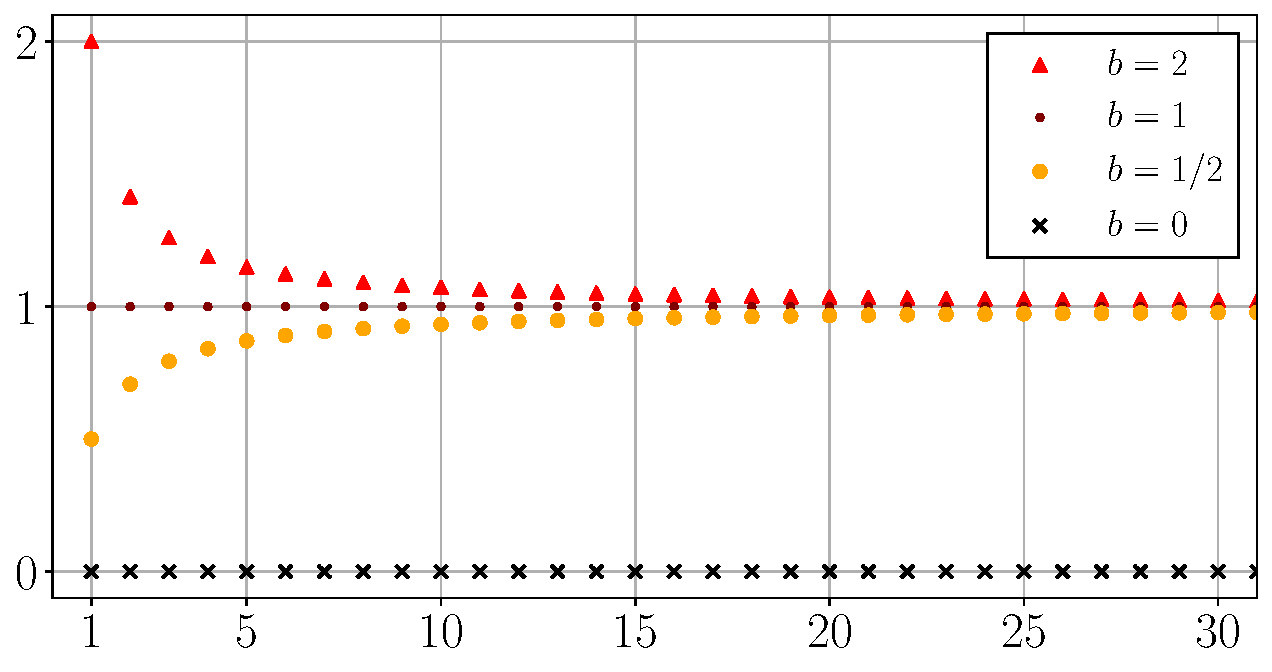
\includegraphics[width=0.8\textwidth]{UA_Figures/UA_ex2_5_6_fig.pdf}
        \caption{\( b^{1/n} \) for \( 1 \leq n \leq 30 \) and \( b = 0, \tfrac{1}{2}, 1, 2 \)}
        \label{fig:ex2.5.6}
    \end{figure}
\end{solution}

\begin{exercise}
\label{ex:2.5.7}
    Extend the result proved in Example 2.5.3 to the case \( \abs{b} < 1 \); that is, show \( \lim (b^n) = 0 \) if and only if \( -1 < b < 1 \).
\end{exercise}

\begin{solution}
    We will consider the following cases.
    \begin{description}
        \item[Case 1.] \( b > 1 \). In this case, \( (b^n) \) is unbounded and hence divergent.

        \item[Case 2.] \( b = 1 \). In this case, \( (b^n) = (1, 1, 1, \ldots) \) and hence \( \lim b^n = 1 \).

        \item[Case 3.] \( 0 < b < 1 \). Example 2.5.3 shows that in this case we have \( \lim b^n = 0 \).

        \item[Case 4.] \( b = 0 \). In this case, \( (b^n) = (0, 0, 0, \ldots) \) and hence \( \lim b^n = 0 \).

        \item[Case 5.] \( -1 < b < 0 \). Observe that \( b = (-1) \abs{b} \), so that \( b^n = (-1)^n \abs{b}^n \). Since \( 0 < \abs{b} < 1 \), we have \( \lim \abs{b}^n = 0 \) by the \( 0 < b < 1 \) case. Given this, and the boundedness of \( (-1)^n \), it follows from \Cref{ex:2.3.9} (a) that
        \[
            \lim b^n = \lim [(-1)^n \abs{b}^n] = 0.
        \]

        \item [Case 6.] \( b = -1 \). In this case \( b^n = (-1)^n \), which is divergent since it has two convergent subsequences with different limits:
        \[
            \lim [(-1)^{2n}] = 1 \neq -1 = \lim [(-1)^{2n+1}].
        \]

        \item[Case 7.] \( b < -1 \). We have \( b^n = (-1)^n \abs{b}^n \) with \( \abs{b} > 1 \). Observe that the subsequence \( (b^{2n}) = \paren{ \abs{b}^{2n} } \) is divergent by the \( b > 1 \) case; it then follows from \Cref{ex:2.5.2} (b) that the sequence \( (b^n) \) is divergent.
    \end{description}
    We may conclude that \( \lim b^n = 0 \) if and only if \( -1 < b < 1 \).
\end{solution}

\begin{exercise}
\label{ex:2.5.8}
    Another way to prove the Bolzano-Weierstrass Theorem is to show that every sequence contains a monotone subsequence. A useful device in this endeavor is the notion of a \textit{peak term}. Given a sequence \( (x_n) \), a particular term \( x_m \) is a peak term if no later term in the sequence exceeds it; i.e., if \( x_m \geq x_n \) for all \( n \geq m \).
    \begin{enumerate}
        \item Find examples of sequences with zero, one, and two peak terms. Find an example of a sequence with infinitely many peak terms that is not monotone.

        \item Show that every sequence contains a monotone subsequence and explain how this furnishes a new proof of the Bolzano-Weierstrass Theorem.
    \end{enumerate}
\end{exercise}

\begin{solution}
    \begin{enumerate}
        \item Any strictly increasing sequence will have zero peak terms; the sequence \( (n) \) for example. For sequences with one and two peak terms, consider (respectively)
        \[
            \paren{ 2, 0, \tfrac{1}{2}, \tfrac{2}{3}, \tfrac{3}{4}, \tfrac{4}{5} \ldots } \hspaceand \paren{ 3, 2, 0, \tfrac{1}{2}, \tfrac{2}{3}, \tfrac{3}{4}, \tfrac{4}{5} \ldots }.
        \]
        For a sequence with infinitely many peak terms but which is not monotone, consider
        \[
            (0, 1, -2, -1, -4, -3, -6, -5, \ldots).
        \]
        See \Cref{fig:ex2.5.8} for a graph of the first thirty terms of these sequences.

        \item Let \( (x_n) \) be a sequence; we will show that \( (x_n) \) contains a monotone subsequence. First, suppose that \( (x_n) \) contains infinitely many peak terms, say \( x_{n_1}, x_{n_2}, \ldots, x_{n_k}, \ldots \), where we may assume that \( n_1 < n_2 < \cdots < n_k < \cdots \); the subsequence \( (x_{n_k}) \) is then a decreasing subsequence of \( (x_n) \). Next, suppose that \( (x_n) \) contains only finitely many peak terms. In this case, we are guaranteed the existence of a term \( x_{n_1} \) which is not a peak term and after which there are no peak terms. Since \( x_{n_1} \) is not a peak term, there exists an \( n_2 > n_1 \) such that \( x_{n_2} > x_{n_1} \) and \( x_{n_2} \) is not a peak term. Since \( x_{n_2} \) is not a peak term, there exists an \( n_3 > n_2 \) such that \( x_{n_3} > x_{n_2} \) and \( x_{n_3} \) is not a peak term. Continuing in this way, we recursively obtain an increasing subsequence \( (x_{n_k}) \) of \( (x_n) \). In either case, we have shown that \( (x_n) \) must contain a monotone subsequence.

        Now suppose that \( (x_n) \) is a bounded sequence. By the previous paragraph, there exists a monotone subsequence \( (x_{n_k}) \), which must also be bounded. The Monotone Convergence Theorem (Theorem 2.4.2) then implies that \( (x_{n_k}) \) is convergent; this provides another proof of the Bolzano-Weierstrass Theorem (Theorem 2.5.5).
    \end{enumerate}
    \begin{figure}[H]
        \centering
        \begin{subfigure}{0.8\textwidth}
            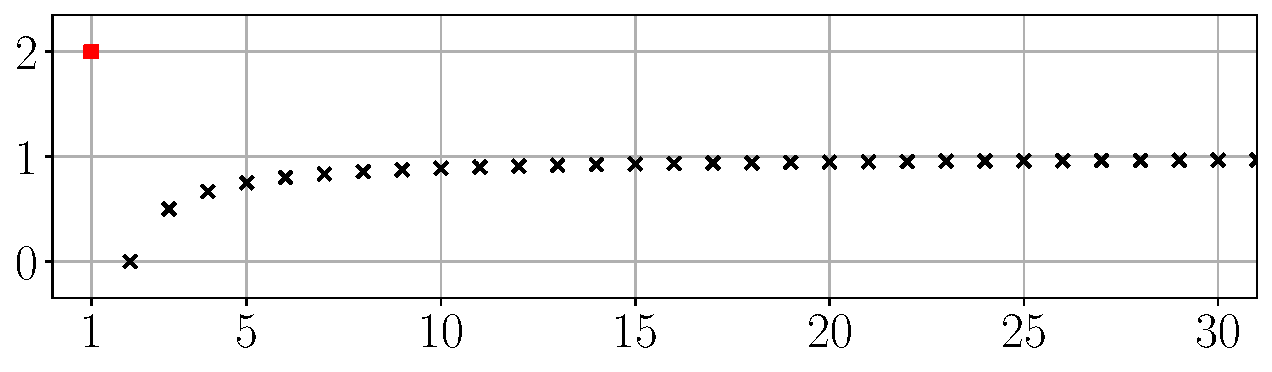
\includegraphics[width=\textwidth]{UA_Figures/UA_ex2_5_8_fig_a.pdf}
            \caption{Sequence with one peak term}
        \end{subfigure} \\
        \begin{subfigure}{0.8\textwidth}
            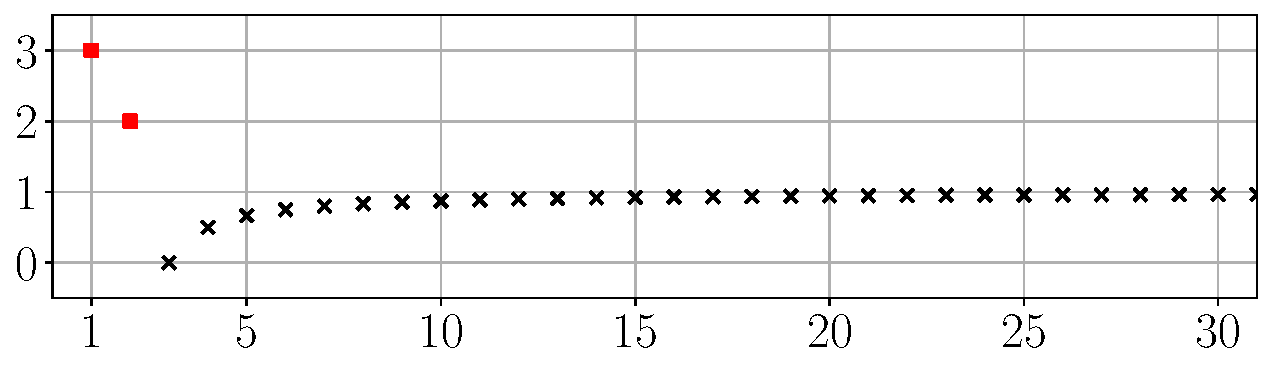
\includegraphics[width=\textwidth]{UA_Figures/UA_ex2_5_8_fig_b.pdf}
            \caption{Sequence with two peak terms}
        \end{subfigure} \\
        \begin{subfigure}{0.8\textwidth}
            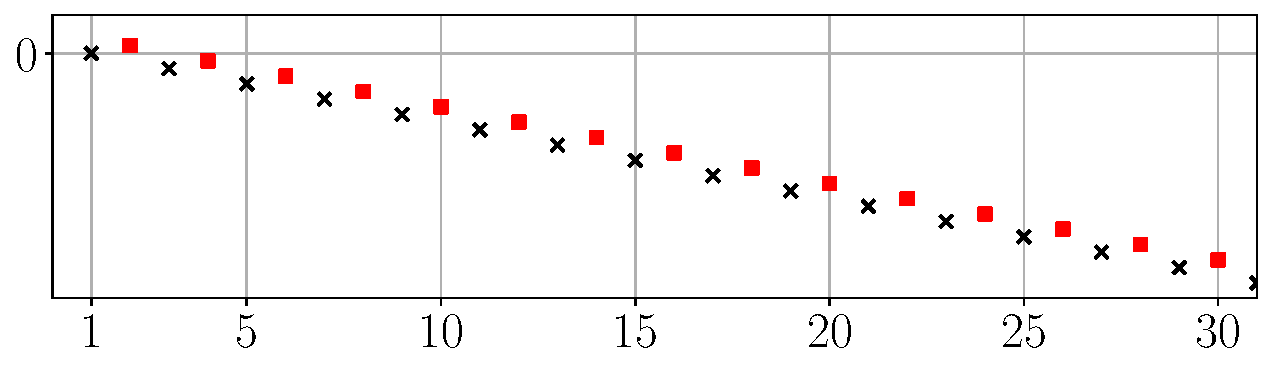
\includegraphics[width=\textwidth]{UA_Figures/UA_ex2_5_8_fig_c.pdf}
            \caption{Non-monotone sequence with infinitely many peak terms}
        \end{subfigure}
        \caption{\Cref{ex:2.5.8} (a) sequences with one, two, and infinitely many peak terms; the red squares indicate peak terms}
        \label{fig:ex2.5.8}
    \end{figure}
\end{solution}

\begin{exercise}
\label{ex:2.5.9}
    Let \( (a_n) \) be a bounded sequence, and define the set
    \[
        S = \{ x \in \R : x < a_n \text{ for infinitely many terms } a_n \}.
    \]
    Show that there exists a subsequence \( (a_{n_k}) \) converging to \( s = \sup S \). (This is a direct proof of the Bolzano-Weierstrass Theorem using the Axiom of Completeness.)
\end{exercise}

\begin{solution}
    Since \( (a_n) \) is bounded, there is an \( M > 0 \) such that \( -M \leq a_n \leq M \) for all \( n \in \N \). It follows that \( (-\infty, -M) \subseteq S \), so that \( S \) is non-empty, and for any \( x \in S \) we have \( x < a_n \leq M \) for some \( n \in \N \), so that \( S \) is bounded above by \( M \). The Axiom of Completeness then implies that \( s := \sup S \) exists in \( \R \).

    Let \( k \) be a positive integer. We claim that the set
    \[
        C_k = \set{ n \in \N : s - \tfrac{1}{k} < a_n \leq s + \tfrac{1}{k} }
    \]
    is infinite. By Lemma 1.3.8, there exists an \( x \in S \) such that \( s - \tfrac{1}{k} < x \leq s \). Define the sets
    \begin{multline*}
        E = \{ n \in \N : x < a_n \}, \quad A_k = \set{ n \in \N : s + \tfrac{1}{k} < a_n } \\[2mm]
        \text{and} \quad B_k = \set{ n \in \N : x < a_n \leq s + \tfrac{1}{k} }.
    \end{multline*}
    Observe that \( E \) is the disjoint union of \( A_k \) and \( B_k \) and that \( E \) is infinite since \( x \in S \). Furthermore, \( A_k \) must be finite, otherwise we would have \( s + \tfrac{1}{k} \in S \). It follows that \( B_k \) is infinite and hence that \( C_k \) is infinite, since \( B_k \subseteq C_k \).

    Since \( C_1 \) is infinite, there exists some \( n_1 \in \N \) such that \( s - 1 < a_{n_1} \leq s + 1 \). Since \( C_2 \) is infinite, there exists some \( n_2 > n_1 \) such that \( s - \tfrac{1}{2} < a_{n_2} \leq s + \tfrac{1}{2} \). We continue this process recursively to obtain a subsequence \( (a_{n_k}) \) satisfying \( s - \tfrac{1}{k} < a_{n_k} \leq s + \tfrac{1}{k} \). The Squeeze Theorem (\Cref{ex:2.3.3}) then implies that \( \lim_{k \to \infty} a_{n_k} = s \).
\end{solution}

\section{The Cauchy Criterion}
\label{sec:2.6}

\begin{exercise}
\label{ex:2.6.1}
    Supply a proof for Theorem 2.6.2.
\end{exercise}

\begin{solution}
    Suppose \( x_n \to x \) for some \( x \in \R \); we will show that \( (x_n) \) is Cauchy. Let \( \epsilon > 0 \) be given. There is an \( N \in \N \) such that \( n \geq N \) implies that \( \abs{x_n - x} < \tfrac{\epsilon}{2} \). For \( m, n \geq N \) we then have
    \[
        \abs{x_n - x_m} \leq \abs{x_n - x} + \abs{x_m - x} < \frac{\epsilon}{2} + \frac{\epsilon}{2} = \epsilon.
    \]
    It follows that \( (x_n) \) is a Cauchy sequence.
\end{solution}

\begin{exercise}
\label{ex:2.6.2}
    Give an example of each of the following, or argue that such a request is impossible.
    \begin{enumerate}
        \item A Cauchy sequence that is not monotone.

        \item A Cauchy sequence with an unbounded subsequence.

        \item A divergent monotone sequence with a Cauchy subsequence.

        \item An unbounded sequence containing a subsequence that is Cauchy.
    \end{enumerate}
\end{exercise}

\begin{solution}
    \begin{enumerate}
        \item Consider the sequence \( (x_n) \) given by \( x_n = \tfrac{(-1)^n}{n} \). The sequence is convergent (\( \lim x_n = 0 \)) and hence Cauchy (Theorem 2.6.4), but is certainly not monotone.
        \begin{figure}[H]
            \centering
            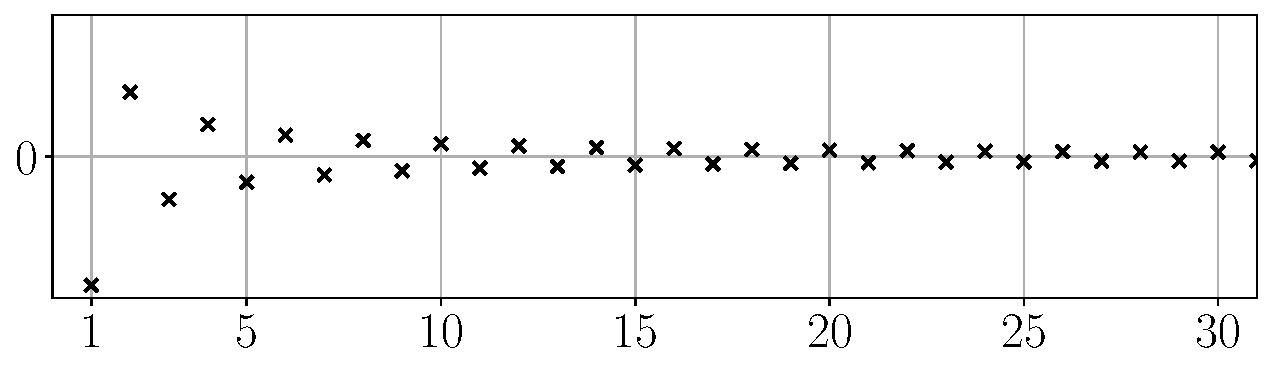
\includegraphics[width=0.8\textwidth]{UA_Figures/UA_ex2_6_2_fig.pdf}
            \caption{\(  \tfrac{(-1)^n}{n} \) for \( 1 \leq n \leq 30 \)}
            \label{fig:ex2.6.2}
        \end{figure}

        \item This is impossible. A Cauchy sequence \( (x_n) \) is necessarily convergent (Theorem 2.6.4) and hence all subsequences of \( (x_n) \) must be convergent (Theorem 2.5.2); each subsequence must then be bounded (Theorem 2.3.2).

        \item First, let us prove the following result.
        \begin{lemma}
        \label{lem:ex2.6.2}
            If \( (x_n) \) is an unbounded monotone sequence, then all subsequences of \( (x_n) \) are also unbounded and monotone.
        \end{lemma}
        \begin{proof}
            Suppose \( (x_n) \) is increasing (the case where \( (x_n) \) is decreasing is handled similarly) and let \( (x_{n_k}) \) be a subsequence of \( (x_n) \). If \( k > \ell \), then \( n_k > n_{\ell} \) and so \( x_{n_k} \geq x_{n_{\ell}} \) since \( (x_n) \) is increasing; it follows that \( (x_{n_k}) \) is an increasing sequence. Now let \( M > 0 \) be given. Since \( (x_n) \) is unbounded, there is an \( N \in \N \) such that \( x_N > M \), and since \( (x_{n_k}) \) is a subsequence of \( (x_n) \) we are guaranteed the existence of a \( K \in \N \) such that \( n_K > N \); it follows that \( x_{n_K} \geq x_N > M \) since \( (x_n) \) is increasing. We may conclude that \( (x_{n_k}) \) is unbounded.
        \end{proof}
        We can now show that the given request is impossible. If \( (x_n) \) is a divergent monotone sequence, then by the Monotone Convergence Theorem (Theorem 2.4.2) the sequence \( (x_n) \) must be unbounded. It follows from \Cref{lem:ex2.6.2} that all subsequences of \( (x_n) \) are unbounded, hence divergent (Theorem 2.3.2), and hence not Cauchy (Theorem 2.6.4).

        \item Consider the unbounded sequence \( (0, 1, 0, 2, 0, 3, \ldots) \); the subsequence \( (0, 0, 0, \ldots) \) is convergent and hence Cauchy (Theorem 2.6.4).
    \end{enumerate}
\end{solution}

\begin{exercise}
\label{ex:2.6.3}
    If \( (x_n) \) and \( (y_n) \) are Cauchy sequences, then one easy way to prove that \( (x_n + y_n) \) is Cauchy is to use the Cauchy Criterion. By Theorem 2.6.4, \( (x_n) \) and \( (y_n) \) must be convergent, and the Algebraic Limit Theorem then implies \( (x_n + y_n) \) is convergent and hence Cauchy.
    \begin{enumerate}
        \item Give a direct argument that \( (x_n + y_n) \) is a Cauchy sequence that does not use the Cauchy Criterion or the Algebraic Limit Theorem.

        \item Do the same for the product \( (x_n y_n) \).
    \end{enumerate}
\end{exercise}

\begin{solution}
    \begin{enumerate}
        \item Let \( \epsilon > 0 \) be given. There are positive integers \( N_1 \) and \( N_2 \) such that
        \[
            m, n \geq N_1 \implies \abs{x_n - x_m} < \frac{\epsilon}{2} \hspaceand m, n \geq N_2 \implies \abs{y_n - y_m} < \frac{\epsilon}{2}.
        \]
        Let \( N = \max \{ N_1, N_2 \} \) and observe that for \( m, n \geq N \) we have
        \[
            \abs{x_n + y_n - x_m - y_m} \leq \abs{x_n - x_m} + \abs{y_n - y_m} < \frac{\epsilon}{2} + \frac{\epsilon}{2} = \epsilon.
        \]
        It follows that \( (x_n + y_n) \) is a Cauchy sequence.

        \item Because Cauchy sequences are bounded (Lemma 2.6.3), there are positive real numbers \( M_1 \) and \( M_2 \) such that \( \abs{x_n} \leq M_1 \) and \( \abs{y_n} \leq M_2 \) for all \( n \in \N \). Let \( \epsilon > 0 \) be given. There are positive integers \( N_1 \) and \( N_2 \) such that
        \[
            m, n \geq N_1 \implies \abs{x_n - x_m} < \frac{\epsilon}{2 M_2} \hspaceand m, n \geq N_2 \implies \abs{y_n - y_m} < \frac{\epsilon}{2 M_1}.
        \]
        Let \( N = \max \{ N_1, N_2 \} \) and observe that for \( m, n \geq N \) we have
        \begin{multline*}
            \abs{x_n y_n - x_m y_m} = \abs{x_n y_n - x_m y_n + x_m y_n - x_m y_m} \leq \abs{y_n} \abs{x_n - x_m} + \abs{x_m} \abs{y_n - y_m} \\[2mm]
            < M_2 \frac{\epsilon}{2 M_2} + M_1 \frac{\epsilon}{2 M_1} = \epsilon.
        \end{multline*}
        It follows that \( (x_n y_n) \) is a Cauchy sequence.
    \end{enumerate}
\end{solution}

\begin{exercise}
\label{ex:2.6.4}
    Let \( (a_n) \) and \( (b_n) \) be Cauchy sequences. Decide whether each of the following sequences is a Cauchy sequence, justifying each conclusion.
    \begin{enumerate}
        \item \( c_n = \abs{a_n - b_n} \)

        \item \( c_n = (-1)^n a_n \)

        \item \( c_n = [[a_n]] \), where \( [[x]] \) refers to the greatest integer less than or equal to \( x \).
    \end{enumerate}
\end{exercise}

\begin{solution}
    By the Cauchy Criterion (Theorem 2.6.4), we have \( \lim a_n = a \) and \( \lim b_n = b \) for some real numbers \( a \) and \( b \). Again by the Cauchy Criterion, it will suffice to consider convergence of the given sequences \( (c_n) \).
    \begin{enumerate}
        \item By \Cref{ex:2.3.10} (b) and the Algebraic Limit Theorem (Theorem 2.3.3), we have
        \[
            \lim c_n = \lim \abs{a_n - b_n} = \abs{ \lim a_n - \lim b_n} = \abs{a - b}.
        \]
        So \( (c_n) \) is convergent and hence Cauchy.

        \item Suppose that \( a = 0 \). By \Cref{ex:2.3.9} (a) we then have \( \lim c_n = 0 \) and it follows that \( (c_n) \) is Cauchy. If \( a \neq 0 \), then observe that
        \[
            \lim c_{2n} = \lim a_{2n} = a \neq -a = \lim (- a_{2n-1}) = \lim c_{2n-1}.
        \]
        So \( (c_n) \) has two subsequences which converge to different limits. It follows that \( (c_n) \) is not convergent (Theorem 2.5.2) and hence not Cauchy.

        \item Suppose that \( a \) is not an integer, so that \( [[a]] < a < [[a]] + 1 \). Let
        \[
            \delta = \min \{ a - [[a]], [[a]] + 1 - a \}.
        \]
        Since \( \lim a_n = a \), there is a positive integer \( N \) such that \( n \geq N \) implies that \( a_n \in (a - \delta, a + \delta) \). Observe that \( [[a]] \leq a - \delta \) and \( a + \delta \leq [[a]] + 1 \). For \( n \geq N \) we then have \( [[a]] < a_n < [[a]] + 1 \), which gives us \( [[a_n]] = [[a]] \). Thus the sequence \( [[a_n]] \) is eventually constant with value \( [[a]] \); it follows that \( [[a_n]] \) is convergent with limit \( [[a]] \) and hence Cauchy.

        If \( a \) is an integer, then the sequence \( ([[a_n]]) \) may or may not be convergent (and so may or may not be Cauchy). For example, if \( (a_n) \) is the sequence \( (0, 0, 0, \ldots) \) then clearly \( \lim [[a_n]] = 0 \). However, consider the sequence \( a_n = \tfrac{(-1)^n}{n} \), which also satisfies \( \lim a_n = 0 \). This gives
        \[
            ([[a_n]]) = (-1, 0, -1, 0, -1, 0, \ldots),
        \]
        which is divergent.
    \end{enumerate}
\end{solution}

\begin{exercise}
\label{ex:2.6.5}
    Consider the following (invented) definition: A sequence \( (s_n) \) is \textit{pseudo-Cauchy} if, for all \( \epsilon > 0 \), there exists an \( N \) such that if \( n \geq N \), then \( \abs{s_{n+1} - s_n} < \epsilon \).

    Decide which one of the following two propositions is actually true. Supply a proof for the valid statement and a counterexample for the other.
    \begin{enumerate}[label = (\roman*)]
        \item Psuedo-Cauchy sequences are bounded.

        \item If \( (x_n) \) and \( (y_n) \) are pseudo-Cauchy, then \( (x_n + y_n) \) is pseudo-Cauchy as well.
    \end{enumerate}
\end{exercise}

\begin{solution}
    \begin{enumerate}[label = (\roman*)]
        \item This statement is false: consider the sequence \( (s_n) \) given by \( s_n = \sum_{m=1}^n \tfrac{1}{m} \). This sequence satisfies \( s_{n+1} - s_n = \tfrac{1}{n+1} \to 0 \), so that \( (s_n) \) is pseudo-Cauchy. However, as shown in Example 2.4.5, \( (s_n) \) is unbounded.

        \item This statement is true. Let \( \epsilon > 0 \) be given. There are positive integers \( N_1 \) and \( N_2 \) such that
        \[
            n \geq N_1 \implies \abs{x_{n+1} - x_n} < \frac{\epsilon}{2} \hspaceand n \geq N_2 \implies \abs{y_{n+1} - y_n} < \frac{\epsilon}{2}.
        \]
        Let \( N = \max \{ N_1, N_2 \} \) and observe that for \( n \geq N \) we have
        \[
            \abs{x_{n+1} + y_{n+1} - x_n - y_n} \leq \abs{x_{n+1} - x_n} + \abs{y_{n+1} - y_n} < \frac{\epsilon}{2} + \frac{\epsilon}{2} = \epsilon.
        \]
        It follows that \( (x_n + y_n) \) is pseudo-Cauchy.
    \end{enumerate}
\end{solution}

\begin{exercise}
\label{ex:2.6.6}
    Let's call a sequence \( (a_n) \) \textit{quasi-increasing} if for all \( \epsilon > 0 \) there exists an \( N \) such that whenever \( n > m \geq N \) it follows that \( a_n > a_m - \epsilon \).
    \begin{enumerate}
        \item Give an example of a sequence that is quasi-increasing but not monotone or eventually monotone.

        \item Give an example of a quasi-increasing sequence that is divergent and not monotone or eventually monotone.

        \item Is there an analogue of the Monotone Convergence Theorem for quasi-increasing sequences? Give an example of a bounded, quasi-increasing sequence that doesn't converge, or prove that no such sequence exists.
    \end{enumerate}
\end{exercise}

\begin{solution}
    \begin{enumerate}
        \item Consider the sequence \( (a_n) \) given by
        \[
            a_n = \begin{cases}
                \tfrac{n+1}{2} & \text{if } n \text{ is odd}, \\
                \tfrac{n}{2} - \tfrac{2}{n} & \text{if } n \text{ is even}.
            \end{cases}
        \]
        \begin{figure}[H]
            \centering
            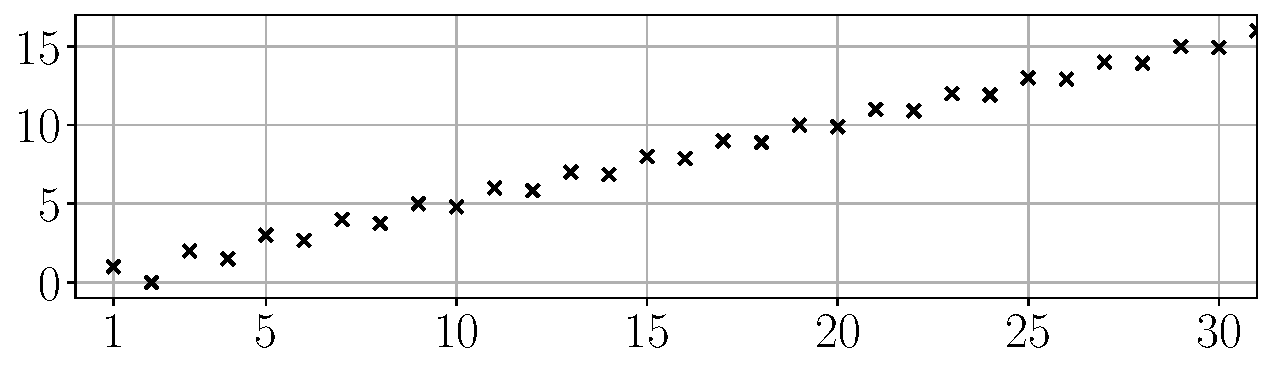
\includegraphics[width=0.8\textwidth]{UA_Figures/UA_ex2_6_6_fig.pdf}
            \caption{\( a_n \) for \( 1 \leq n \leq 30 \)}
            \label{fig:ex2.6.6}
        \end{figure}
        \noindent Some calculations reveal that this sequence has the following properties.
        \begin{enumerate}[label=(\roman*)]
            \item If \( m \in \N \) is even, then \( a_n > a_m \) for all \( n > m \).

            \item If \( m \in \N \) is odd, then \( a_n > a_m \) for all \( n > m + 1 \) and \( a_m - a_{m+1} = \tfrac{2}{m+1} > 0 \).
        \end{enumerate}
        It follows that \( (a_n) \) is not eventually monotone, for if \( N \) is a positive integer, choose an odd integer \( m \) such that \( m > N \); by property (ii) we then have \( a_m > a_{m+1} \) and \( a_m < a_{m+2} \). Furthermore, \( (a_n) \) is quasi-increasing. To see this, let \( \epsilon > 0 \) be given. Choose a positive integer \( N \) such that \( \tfrac{2}{N+1} < \epsilon \) and suppose that \( n > m \geq N \). By properties (i) and (ii), we have
        \[
            a_m - a_n < 0 < \epsilon \implies a_n > a_m - \epsilon
        \]
        unless \( m \) is odd and \( n = m + 1 \). In that case we have
        \[
            a_m - a_{m+1} = \frac{2}{m+1} \leq \frac{2}{N+1} < \epsilon \implies a_n > a_m - \epsilon.
        \]

        \item The sequence \( (a_n) \) given in part (a) is unbounded and hence divergent.

        \item There is an analogue of the Monotone Convergence Theorem (Theorem 2.4.2) for bounded quasi-increasing sequences. Let \( (a_n) \) be such a sequence; we will show that \( (a_n) \) converges to \( \limsup a_n \).

        Let \( s = \limsup a_n \) and \( y_n = \sup \{ a_{\ell} : \ell \geq n \} \), so that \( \lim y_n = s \). By \Cref{ex:2.5.2} (c), there is a subsequence \( (a_{n_k}) \) converging to \( s \). Let \( \epsilon > 0 \) be given. There is an \( N_1 \in \N \) such that \( \abs{y_n - s} < \epsilon \) whenever \( n \geq N_1 \). Since \( a_n \leq y_n \) for all \( n \in \N \), we have
        \[
            n \geq N_1 \implies a_n < s + \epsilon. \tag{1}
        \]
        Since \( (a_n) \) is quasi-increasing, there is an \( N_2 \in \N \) such that
        \[
            n > m \geq N_2 \implies a_m - \frac{\epsilon}{2} < a_n, \tag{2}
        \]
        and since \( (a_{n_k}) \to s \), there is a \( K \in \N \) such that
        \[
            k \geq K \implies \abs{a_{n_k} - s} < \frac{\epsilon}{2}. \tag{3}
        \]
        Because \( (a_{n_k}) \) is a subsequence, there must be some \( k' \in \N \) such that both \( k' \geq K \) and \( n_{k'} \geq N_2 \). It follows that
        \[
            n > n_{k'} \implies a_{n_{k'}} - \frac{\epsilon}{2} < a_n \qquad \text{by } (2),
        \]
        and \( s - \epsilon < a_{n_{k'}} - \tfrac{\epsilon}{2} \) by (3). Combining these gives
        \[
            n > n_{k'} \implies s - \epsilon < a_n. \tag{4}
        \]
        Let \( N = \max \{ N_1, n_{k'} \} \). By (1) and (4), we then have
        \[
            n > N \implies s - \epsilon < a_n < s + \epsilon.
        \]
        It follows that \( \lim a_n = s \).
    \end{enumerate}
\end{solution}

\begin{exercise}
\label{ex:2.6.7}
    \Cref{ex:2.4.4,ex:2.5.4} establish the equivalence of the Axiom of Completeness and the Monotone Convergence Theorem. They also show that the Nested Interval Property is equivalent to these other two in the presence of the Archimedean Property.
    \begin{enumerate}
        \item Assume the Bolzano-Weierstrass Theorem is true and use it to construct a proof of the Monotone Convergence Theorem without making any appeal to the Archimedean Property. This shows that BW, AoC, and MCT are all equivalent.

        \item Use the Cauchy Criterion to prove the Bolzano-Weierstrass Theorem, and find the point in the argument where the Archimedean Property is implicitly required. This establishes the final link in the equivalence of the five characterizations of completeness discussed at the end of Section 2.6.

        \item How do we know it is impossible to prove the Axiom of Completeness starting from the Archimedean Property?
    \end{enumerate}
\end{exercise}

\begin{solution}
    \begin{enumerate}
        \item Suppose \( (x_n) \) is bounded and increasing (the case where \( (x_n) \) is decreasing is handled similarly). By assumption, there is a convergent subsequence \( (x_{n_k}) \), say \( \lim_{k \to \infty} x_{n_k} = x \) for some \( x \in \R \). Let \( \epsilon > 0 \) be given. There is a \( K \in \N \) such that
        \[
            k \geq K \implies \abs{x_{n_k} - x} < \epsilon. \tag{1}
        \]
        Suppose \( n \in \N \) is such that \( n \geq n_K \). Since \( (x_n) \) is increasing, we then have \( x - \epsilon < x_{n_K} \leq x_n \). Furthermore, it must be the case that \( x_n < x + \epsilon \). Indeed, if \( x_n \geq x + \epsilon \), then since \( (x_{n_k}) \) is a subsequence there must be some \( k \in \N \) such that \( n_k \geq n \geq n_K \). This implies that \( k \geq K \) and, since \( (x_n) \) is increasing, that \( x_{n_k} \geq x_n \geq x + \epsilon \); this contradicts (1). So we have shown that
        \[
            n \geq n_K \implies x - \epsilon < x_n < x + \epsilon.
        \]
        It follows that \( \lim x_n = x \).

        \item Let \( (x_n) \) be a sequence bounded by some \( M > 0 \). As in the proof of the Bolzano-Weierstrass Theorem (Theorem 2.5.5) given in the textbook, construct a sequence of nested intervals \( (I_k) \) with length \( M \cdot 2^{-k+1} \) and a subsequence \( (x_{n_k}) \) such that \( x_{n_k} \in I_k \). Let \( \epsilon > 0 \) be given. Assuming that \( 2^{-k} \to 0 \) (this is equivalent to assuming the Archimedean Property (Theorem 1.4.2)), there is a \( K \in \N \) such that \( M \cdot 2^{-K+1} < \epsilon \). Suppose that \( k > \ell \geq K \). Since the intervals are nested, both \( x_{n_k} \) and \( x_{n_{\ell}} \) belong to \( I_K \). It follows that \( x_{n_k} \) and \( x_{n_{\ell}} \) are no further apart than the width of \( I_K \), i.e.,
        \[
            \abs{x_{n_k} - x_{n_{\ell}}} \leq \frac{M}{2^{K-1}} < \epsilon.
        \]
        This demonstrates that \( (x_{n_k}) \) is a Cauchy sequence. By assumption, this is equivalent to \( (x_{n_k}) \) being convergent.

        \item The ordered field \( \Q \) has the Archimedean Property but does not satisfy the Axiom of Completeness (see \Cref{lem:ex1.3.10}; the subset \( A \subseteq \Q \) given there is non-empty and bounded above but has no supremum in \( \Q \)).
    \end{enumerate}
\end{solution}

\section{Properties of Infinite Series}
\label{sec:2.7}

\begin{exercise}
\label{ex:2.7.1}
    Proving the Alternating Series Test (Theorem 2.7.7) amounts to showing that the sequence of partial sums
    \[
        s_n = a_1 - a_2 + a_3 - \cdots \pm a_n
    \]
    converges. (The opening example in Section 2.1 includes a typical illustration of \( (s_n) \).) Different characterizations of completeness lead to different proofs.
    \begin{enumerate}
        \item Prove the Alternating Series Test by showing that \( (s_n) \) is a Cauchy sequence.

        \item Supply another proof for this result using the Nested Interval Property (Theorem 1.4.1).

        \item Consider the subsequences \( (s_{2n}) \) and \( (s_{2n+1}) \), and show how the Monotone Convergence Theorem leads to a third proof for the Alternating Series Test.
    \end{enumerate}
\end{exercise}

\begin{solution}
    First note that since \( (a_n) \) is decreasing and converges to zero, \( a_n \geq 0 \) and \( a_n - a_{n+1} \geq 0 \) for all \( n \in \N \).
    \begin{enumerate}
        \item Suppose \( n > m \) are positive integers. If \( n - m \) is even, then
        \[
            s_n - s_m = \underbrace{a_{m+1} - a_{m+2}}_{\geq 0} + \underbrace{a_{m+3} - a_{m+4}}_{\geq 0} + \cdots + \underbrace{a_{n-1} - a_n}_{\geq 0} \geq 0,
        \]
        and if \( n - m \) is odd, then
        \[
            s_n - s_m = \underbrace{a_{m+1} - a_{m+2}}_{\geq 0} + \underbrace{a_{m+3} - a_{m+4}}_{\geq 0} + \cdots + \underbrace{a_{n-2} - a_{n-1}}_{\geq 0} + \underbrace{a_n}_{\geq 0} \geq 0.
        \]
        It follows that \( \abs{s_n - s_m} = s_n - s_m = a_{m+1} - a_{m+2} + \cdots \pm a_n \). If \( n - m \) is even, then
        \[
            \abs{s_n - s_m} = a_{m+1} + \underbrace{(-a_{m+2} + a_{m+3})}_{\leq 0} + \cdots + \underbrace{(-a_{n-2} + a_{n-1})}_{\leq 0} + \underbrace{(-a_n)}_{\leq 0} \leq a_{m+1},
        \]
        and if \( n - m \) is odd, then
        \[
            \abs{s_n - s_m} = a_{m+1} + \underbrace{(-a_{m+2} + a_{m+3})}_{\leq 0} + \cdots + \underbrace{(-a_{n-1} + a_n)}_{\leq 0} \leq a_{m+1}.
        \]
        It follows that \( \abs{s_n - s_m} \leq a_{m+1} \). Let \( \epsilon > 0 \) be given. Since \( a_n \to 0 \), there is an \( N \in \N \) such that \( \abs{a_n} = a_n < \epsilon \) for all \( n \geq N \). For \( n > m \geq N \) we then have
        \[
            \abs{s_n - s_m} \leq a_{m+1} < \epsilon.
        \]
        It follows that \( (s_n) \) is a Cauchy sequence.

        \item Let \( n \) be a positive integer. Observe that
        \begin{align*}
            s_{2n-1} - s_{2n} = a_{2n} \geq 0 &\implies s_{2n} \leq s_{2n-1}, \\[2mm]
            s_{2n-1} - s_{2n-3} = a_{2n-1} - a_{2n-2} \leq 0 &\implies s_{2n-1} \leq s_{2n-3}, \\[2mm]
            s_{2n} - s_{2n-2} = a_{2n-1} - a_{2n} \geq 0 &\implies s_{2n-2} \leq s_{2n}.
        \end{align*}
        Thus \( (I_n = [s_{2n}, s_{2n-1}])_{n=1}^{\infty} \) is a sequence of nested intervals. It follows from the Nested Interval Property (Theorem 1.4.1) that there exists some \( x \in \bigcap_{n=1}^{\infty} I_n \); we claim that \( \lim s_n = x \). To see this, suppose that \( n \in \N \). If \( n \) is even, then \( s_n \in I_{n/2} = [s_n, s_{n-1}] \) and so
        \[
            \abs{s_n - x} \leq \abs{I_{n/2}} = s_{n-1} - s_n = a_n.
        \]
        If \( n \) is odd, then \( s_n \in I_{(n+1)/2} = [s_{n+1}, s_n] \) and so
        \[
            \abs{s_n - x} \leq \abs{I_{(n+1)/2}} = s_n - s_{n+1} = a_{n+1} \leq a_n.
        \]
        It follows that for all \( n \in \N \) we have \( \abs{s_n - x} \leq a_n \); since \( a_n \to 0 \), an application of the Squeeze Theorem (\Cref{ex:2.3.3}) then yields \( \lim s_n = x \).

        \item As shown in (b), the sequence \( (s_{2n}) \) is increasing and bounded above by \( s_1 \), and the sequence \( (s_{2n+1}) \) is decreasing and bounded below by \( s_2 \). The Monotone Convergence Theorem (Theorem 2.4.2) then implies that \( \lim s_{2n} \) and \( \lim s_{2n+1} \) both exist. The relationship \( s_{2n+1} - s_{2n} = a_{2n+1} \) gives
        \[
            \lim (s_{2n+1} - s_{2n}) = \lim a_{2n+1} = 0,
        \]
        so that \( (s_{2n}) \) and \( (s_{2n+1}) \) both converge to the same limit \( x \in \R \) (\Cref{ex:2.3.10} (c)). It follows that \( \lim s_n = x \), as the next lemma shows.
        \begin{lemma}
        \label{lem:ex2.7.1}
            If \( (x_n) \) is a sequence of real numbers such that
            \[
                \lim x_{2n} = \lim x_{2n+1} = x
            \]
            for some \( x \in \R \), then \( \lim x_n = x \).
        \end{lemma}
        \begin{proof}
            Let \( \epsilon > 0 \) be given. There are positive integers \( N_1 \) and \( N_2 \) such that
            \begin{gather*}
                n \geq N_1 \implies \abs{x_{2n} - x} < \epsilon, \tag{1} \\
                n \geq N_2 \implies \abs{x_{2n+1} - x} < \epsilon. \tag{2}
            \end{gather*}
            Let \( N = \max \{ N_1, N_2 \} \) and suppose that \( n \in \N \) is such that \( n \geq 2N + 1 \). If \( n \) is even, then \( \tfrac{n}{2} > N \geq N_1 \) and so \( \abs{x_n - x} < \epsilon \) by (1). If \( n \) is odd, then \( \tfrac{n-1}{2} \geq N \geq N_2 \) and so \( \abs{x_n - x} < \epsilon \) by (2). Thus
            \[
                n \geq 2N + 1 \implies \abs{x_n - x} < \epsilon.
            \]
            It follows that \( \lim x_n = x \).
        \end{proof}
    \end{enumerate}
\end{solution}

\begin{exercise}
\label{ex:2.7.2}
    Decide whether each of the following series converges or diverges:

    \vspace{3mm}
    \hspace{-4.5mm}
    \( \text{(a)} \, \sum_{n=1}^{\infty} \tfrac{1}{2^n + n} \qquad \text{(b)} \, \sum_{n=1}^{\infty} \tfrac{\sin(n)}{n^2} \)
    \begin{enumerate}[start = 3]
        \item \( 1 - \tfrac{3}{4} + \tfrac{4}{6} - \tfrac{5}{8} + \tfrac{6}{10} - \tfrac{7}{12} + \cdots \)

        \item \( 1 + \tfrac{1}{2} - \tfrac{1}{3} + \tfrac{1}{4} + \tfrac{1}{5} - \tfrac{1}{6} + \tfrac{1}{7} + \tfrac{1}{8} - \tfrac{1}{9} + \cdots \)

        \item \( 1 - \tfrac{1}{2^2} + \tfrac{1}{3} - \tfrac{1}{4^2} + \tfrac{1}{5} - \tfrac{1}{6^2} + \tfrac{1}{7} - \tfrac{1}{8^2} + \cdots \)
    \end{enumerate}
\end{exercise}

\begin{solution}
    See \Cref{fig:ex2.7.2} for graphs of the first thirty terms of relevant partial sums for each series.
    \begin{enumerate}
        \item Observe that for each \( n \in \N \) we have
        \[
            0 < \frac{1}{2^n + n} < \frac{1}{2^n}.
        \]
        Since \( \sum_{n=1}^{\infty} \tfrac{1}{2^n} = 1 \) (Example 2.7.5), the Comparison Test (Theorem 2.7.4) implies that \( \sum_{n=1}^{\infty} \tfrac{1}{2^n + n} \) is convergent.

        \item Observe that for each \( n \in \N \) we have
        \[
            0 < \frac{\abs{\sin(n)}}{n^2} \leq \frac{1}{n^2}.
        \]
        Since \( \sum_{n=1}^{\infty} \tfrac{1}{n^2} \) is convergent (Example 2.4.4), the Comparison Test (Theorem 2.7.4) implies that \( \sum_{n=1}^{\infty} \tfrac{\sin(n)}{n^2} \) is absolutely convergent and hence convergent (Theorem 2.7.6).

        \item This is the series \( \sum_{n=1}^{\infty} a_n \), where
        \[
            a_n = (-1)^{n+1} \frac{n + 1}{2n} = (-1)^{n+1} \paren{ \frac{1}{2} + \frac{1}{2n} }.
        \]
        The sequence \( (a_n) \) is divergent by Theorem 2.5.2:
        \[
            \lim a_{2n} = -\frac{1}{2} \neq \frac{1}{2} = \lim a_{2n+1}.
        \]
        It follows from Theorem 2.7.3 that \( \sum_{n=1}^{\infty} a_n \) is divergent.

        \item For the series \( 1 + \tfrac{1}{2} - \tfrac{1}{3} + \tfrac{1}{4} + \tfrac{1}{5} - \tfrac{1}{6} + \tfrac{1}{7} + \tfrac{1}{8} - \tfrac{1}{9} + \cdots \), let \( (s_n) \) be the sequence of partial sums and consider the subsequence \( (s_{3n}) \). Observe that
        \begin{align*}
            s_{3n} = \,\, & \paren{ 1 + \frac{1}{2} - \frac{1}{3} } + \paren{ \frac{1}{4} + \frac{1}{5} - \frac{1}{6} } + \cdots + \paren{ \frac{1}{3n - 2} + \frac{1}{3n - 1} - \frac{1}{3n} } \\[2mm]
            \geq \,\, & \paren{ 1 + \frac{1}{2} - \frac{1}{2} } + \paren{ \frac{1}{4} + \frac{1}{5} - \frac{1}{5} } + \cdots + \paren{ \frac{1}{3n - 2} + \frac{1}{3n - 1} - \frac{1}{3n - 1} } \\[2mm]
            = \,\, & 1 + \frac{1}{4} + \cdots + \frac{1}{3n - 2} \\[2mm]
            = \,\, & \frac{1}{3} \sum_{k=1}^n \frac{1}{k - \tfrac{2}{3}} \\[2mm]
            \geq \,\, & \frac{1}{3} \sum_{k=1}^n \frac{1}{k}.
        \end{align*}
        So we have shown that \( s_{3n} \geq \tfrac{1}{3} \sum_{k=1}^n \tfrac{1}{k} \) for all \( n \in \N \). Since \( \sum_{k=1}^n \tfrac{1}{k} \) is unbounded in \( n \) (Example 2.4.5), it follows that \( (s_{3n}) \) is unbounded. This implies that \( (s_n) \) is unbounded and hence divergent (Theorem 2.3.2).

        \item For the series \( 1 - \tfrac{1}{2^2} + \tfrac{1}{3} - \tfrac{1}{4^2} + \tfrac{1}{5} - \tfrac{1}{6^2} + \tfrac{1}{7} - \tfrac{1}{8^2} + \cdots \), let \( (s_n) \) be the sequence of partial sums and consider the subsequence \( (s_{2n}) \). For any \( m \geq 2 \), we have
        \[
            \frac{1}{m^2} \leq \frac{1}{m(m-1)} = \frac{1}{m-1} - \frac{1}{m} \implies -\frac{1}{m^2} \geq - \frac{1}{m-1} + \frac{1}{m}.
        \]
        It follows that
        \begin{align*}
            s_{2n} = \,\, & \paren{ 1 - \frac{1}{2^2} } + \paren{ \frac{1}{3} - \frac{1}{4^2} } + \cdots + \paren{ \frac{1}{2n - 1} - \frac{1}{(2n)^2} } \\[2mm]
            \geq \,\, & \paren{ 1 - 1 + \frac{1}{2} } + \paren{ \frac{1}{3} - \frac{1}{3} + \frac{1}{4} } + \cdots + \paren{ \frac{1}{2n-1} - \frac{1}{2n-1} + \frac{1}{2n} } \\[2mm]
            = \,\, & \frac{1}{2} + \frac{1}{4} + \cdots + \frac{1}{2n} \\[2mm]
            = \,\, & \frac{1}{2} \sum_{k=1}^n \frac{1}{k}.
        \end{align*}
        So we have shown that \( s_{2n} \geq \tfrac{1}{2} \sum_{k=1}^n \tfrac{1}{k} \) for all \( n \in \N \). Since \( \sum_{k=1}^n \tfrac{1}{k} \) is unbounded in \( n \) (Example 2.4.5), it follows that \( (s_{2n}) \) is unbounded. This implies that \( (s_n) \) is unbounded and hence divergent (Theorem 2.3.2).
    \end{enumerate}
    \begin{figure}[H]
        \centering
        \begin{subfigure}{0.85\textwidth}
            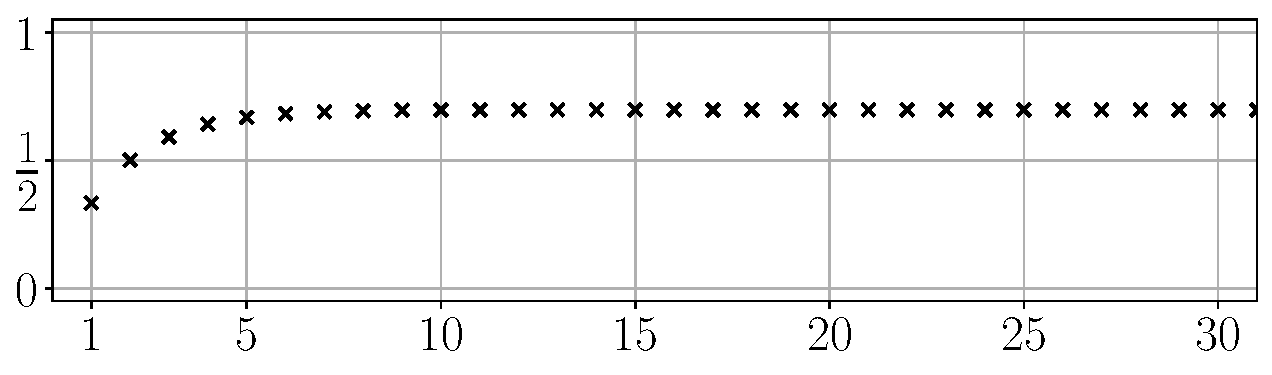
\includegraphics[width=\textwidth]{UA_Figures/UA_ex2_7_2_fig_a.pdf}
            \caption{\( \sum_{k=1}^n \tfrac{1}{2^k + k} \) for \( 1 \leq n \leq 30 \)}
        \end{subfigure}
        \caption{\Cref{ex:2.7.2} partial sums for \( 1 \leq n \leq 30 \)}
    \end{figure}

    \begin{figure}[H]\ContinuedFloat
        \centering
        \begin{subfigure}{0.85\textwidth}
            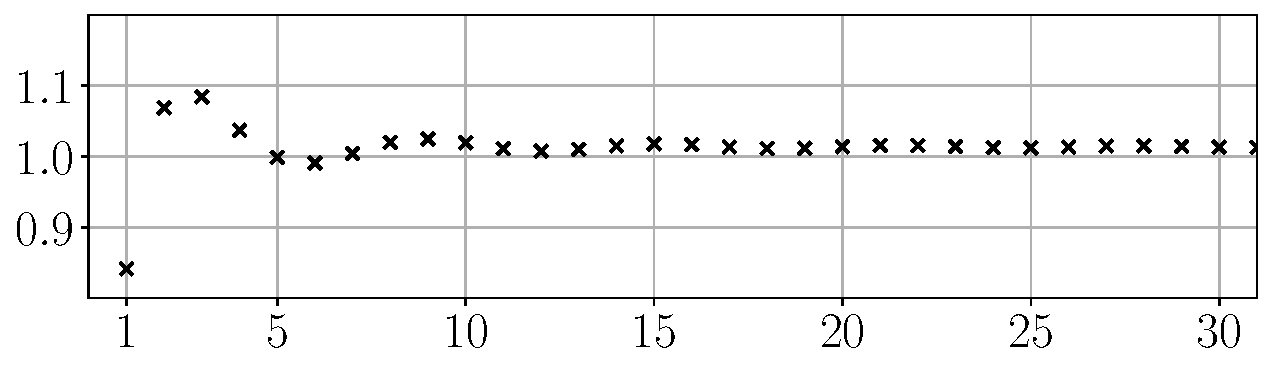
\includegraphics[width=\textwidth]{UA_Figures/UA_ex2_7_2_fig_b.pdf}
            \caption{\( \sum_{k=1}^n \frac{\sin(k)}{k^2} \) for \( 1 \leq n \leq 30 \)}
        \end{subfigure} \\
        \begin{subfigure}{0.85\textwidth}
            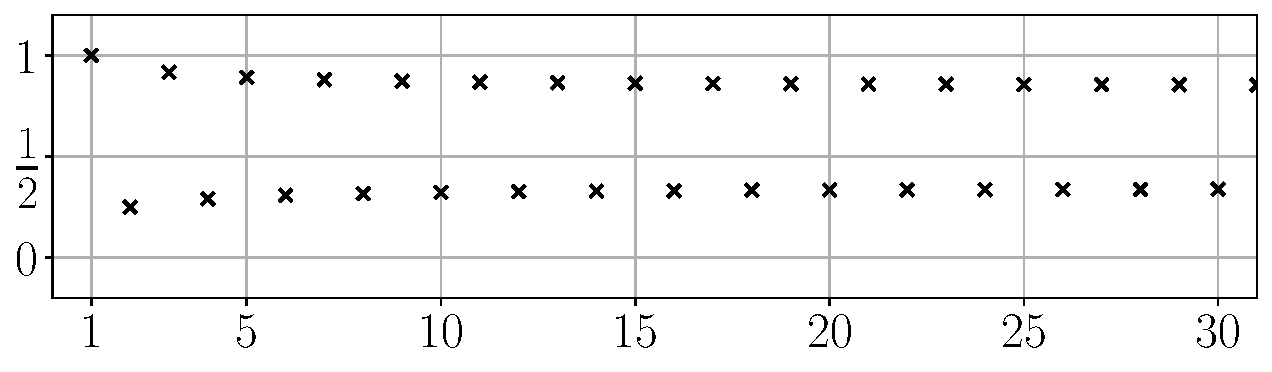
\includegraphics[width=\textwidth]{UA_Figures/UA_ex2_7_2_fig_c.pdf}
            \caption{\( \sum_{k=1}^n (-1)^{k+1} \frac{k + 1}{2k} \) for \( 1 \leq n \leq 30 \)}
        \end{subfigure} \\
        \begin{subfigure}{0.85\textwidth}
            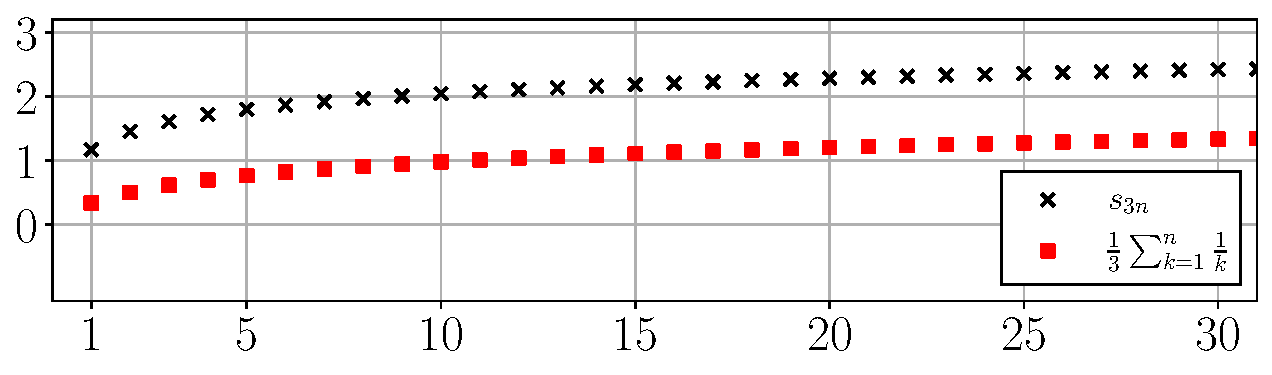
\includegraphics[width=\textwidth]{UA_Figures/UA_ex2_7_2_fig_d.pdf}
            \caption{\( s_{3n} \) and \( \tfrac{1}{3} \sum_{k=1}^n \frac{1}{k} \) for \( 1 \leq n \leq 30 \)}
        \end{subfigure} \\
        \begin{subfigure}{0.85\textwidth}
            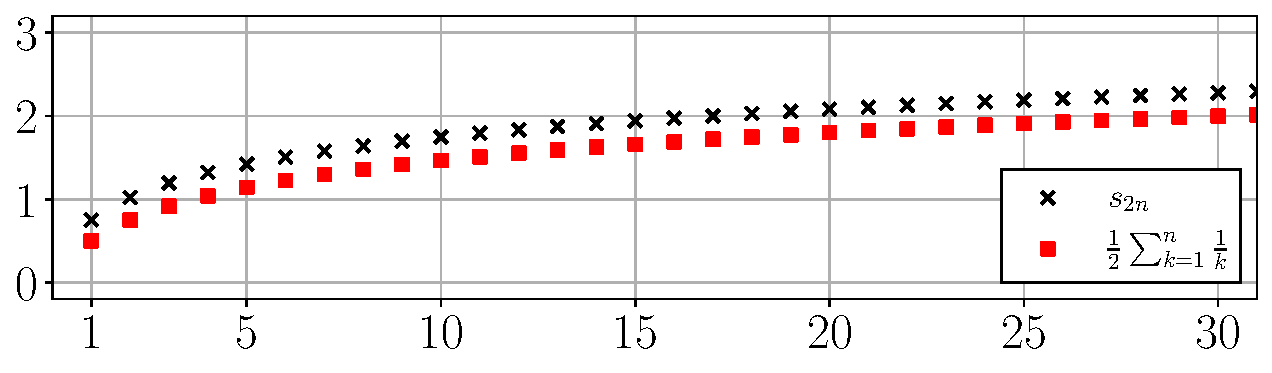
\includegraphics[width=\textwidth]{UA_Figures/UA_ex2_7_2_fig_e.pdf}
            \caption{\( s_{2n} \) and \( \tfrac{1}{2} \sum_{k=1}^n \frac{1}{k} \) for \( 1 \leq n \leq 30 \)}
        \end{subfigure}
        \caption{\Cref{ex:2.7.2} partial sums for \( 1 \leq n \leq 30 \) (cont.)}
        \label{fig:ex2.7.2}
    \end{figure}
\end{solution}

\begin{exercise}
\label{ex:2.7.3}
    \begin{enumerate}
        \item Provide the details for the proof of the Comparison Test (Theorem 2.7.4) using the Cauchy Criterion for Series.

        \item Give another proof for the Comparison Test, this time using the Monotone Convergence Theorem.
    \end{enumerate}
\end{exercise}

\begin{solution}
    \begin{enumerate}
        \item Since \( 0 \leq a_k \leq b_k \) for all \( k \in \N \), for any \( n > m \) we have
        \[
            \abs{a_{m+1} + \cdots + a_n} = a_{m+1} + \cdots + a_n \leq b_{m+1} + \cdots + b_n = \abs{b_{m+1} + \cdots + b_n}. \tag{1}
        \]
        Suppose that \( \sum_{k=1}^{\infty} b_k \) is convergent and let \( \epsilon > 0 \) be given. By the Cauchy Criterion for Series (Theorem 2.7.2), there exists an \( N \in \N \) such that
        \[
            n > m \geq N \implies \abs{b_{m+1} + \cdots + b_n} < \epsilon.
        \]
        It then follows from inequality (1) that \( \abs{a_{m+1} + \cdots + a_n} < \epsilon \) for all \( n > m \geq N \). The Cauchy Criterion for Series (Theorem 2.7.2) allows us to conclude that \( \sum_{k=1}^{\infty} a_k \) is convergent.

        Now suppose that \( \sum_{k=1}^{\infty} a_k \) is divergent. By the Cauchy Criterion for Series (Theorem 2.7.2), there must exist an \( \epsilon > 0 \) such that for all \( N \in \N \) there are positive integers \( n \) and \( m \) such that
        \[
            n > m \geq N \hspaceand \abs{a_{m+1} + \cdots + a_n} \geq \epsilon.
        \]
        Let \( N \in \N \) be given and let \( n \) and \( m \) be the positive integers obtained above. Inequality (1) then gives us \( \abs{b_{m+1} + \cdots + b_n} \geq \epsilon \); it follows from the Cauchy Criterion for Series (Theorem 2.7.2) that \( \sum_{k=1}^{\infty} b_k \) is divergent.

        \item Define the sequences of partial sums
        \[
            s_n = a_1 + \cdots + a_n \hspaceand t_n = b_1 + \cdots + b_n.
        \]
        Since \( 0 \leq a_k \leq b_k \) for all \( k \in \N \), both sequences of partial sums are increasing and satisfy \( 0 \leq s_n \leq t_n \) for all \( n \in \N \). It follows from the Monotone Convergence Theorem (Theorem 2.4.2) that the convergence of each sequence is equivalent to the boundedness of that sequence. From the inequality \( 0 \leq s_n \leq t_n \), it is clear that \( (s_n) \) is bounded if \( (t_n) \) is bounded and that \( (t_n) \) is unbounded if \( (s_n) \) is unbounded.
    \end{enumerate}
\end{solution}

\begin{exercise}
\label{ex:2.7.4}
    Give an example of each or explain why the request is impossible referencing the proper theorem(s).
    \begin{enumerate}
        \item Two series \( \sum x_n \) and \( \sum y_n \) that both diverge but where \( \sum x_n y_n \) converges.

        \item A convergent series \( \sum x_n \) and a bounded sequence \( (y_n) \) such that \( \sum x_n y_n \) diverges.

        \item Two sequences \( (x_n) \) and \( (y_n) \) where \( \sum x_n \) and \( \sum (x_n + y_n) \) both converge but \( \sum y_n \) diverges.

        \item A sequence \( (x_n) \) satisfying \( 0 \leq x_n \leq 1/n \) where \( \sum (-1)^n x_n \) diverges.
    \end{enumerate}
\end{exercise}

\begin{solution}
    \begin{enumerate}
        \item If we let \( (x_n) \) and \( (y_n) \) be the sequences given by \( x_n = y_n = \tfrac{1}{n} \), then \( \sum_{n=1}^{\infty} x_n = \sum_{n=1}^{\infty} y_n = \sum_{n=1}^{\infty} \tfrac{1}{n} \) is the divergent harmonic series (Example 2.4.5), but \( \sum_{n=1}^{\infty} x_n y_n = \sum_{n=1}^{\infty} \tfrac{1}{n^2} \) is convergent (Example 2.4.4).

        \item Let \( (x_n) \) be the sequence given by \( x_n = \tfrac{(-1)^{n+1}}{n} \) and \( (y_n) \) be the bounded sequence given by \( y_n = (-1)^{n+1} \). It then follows from the Alternating Series Test (Theorem 2.7.7) that \( \sum_{n=1}^{\infty} x_n \) is convergent, but \( \sum_{n=1}^{\infty} x_n y_n = \sum_{n=1}^{\infty} \tfrac{1}{n} \) is the divergent harmonic series (Example 2.4.5).

        \item This is impossible; by Theorem 2.7.1 we must have
        \[
            \sum_{n=1}^{\infty} y_n = \sum_{n=1}^{\infty} (x_n + y_n) - \sum_{n=1}^{\infty} x_n.
        \]

        \item Let \( (x_n) \) be the sequence given by
        \[
            x_n = \begin{cases}
                \frac{1}{2(n+1)} & \text{if } n \text{ is odd}, \\
                \frac{1}{n} & \text{if } n \text{ is even},
            \end{cases}
            \quad \text{i.e., } (x_n) = \paren{ \frac{1}{4}, \frac{1}{2}, \frac{1}{8}, \frac{1}{4}, \frac{1}{12}, \frac{1}{6}, \ldots },
        \]
        so that \( 0 \leq x_n \leq \tfrac{1}{n} \) for all \( n \in \N \), and let \( (s_n) \) be the sequence of partial sums for the series \( \sum_{n=1}^{\infty} (-1)^n x_n \). Observe that
        \begin{align*}
            s_{2n} &= \paren{ -\frac{1}{4} + \frac{1}{2} } + \paren{ -\frac{1}{8} + \frac{1}{4} } + \cdots + \paren{ -\frac{1}{4n} + \frac{1}{2n} } \\[2mm]
            &= \frac{1}{4} + \frac{1}{8} + \cdots + \frac{1}{4n} \\[2mm]
            &= \frac{1}{4} \sum_{k=1}^n \frac{1}{k}.
        \end{align*}
        It follows that \( (s_{2n}) \) is unbounded (Example 2.4.5) and hence that \( \sum_{n=1}^{\infty} (-1)^n x_n \) is divergent.
    \end{enumerate}
\end{solution}

\begin{exercise}
\label{ex:2.7.5}
    Now that we have proved the basic facts about geometric series, supply a proof for Corollary 2.4.7.
\end{exercise}

\begin{solution}
    We want to show that the series \( \sum_{n=1}^{\infty} \tfrac{1}{n^p} \) converges if and only if \( p > 1 \). If \( p \leq 0 \), then \( \tfrac{1}{n^p} \) does not converge to zero; it follows that \( \sum_{n=1}^{\infty} \tfrac{1}{n^p} \) diverges (Theorem 2.7.3). Suppose that \( p > 0 \) and notice that the sequence \( \tfrac{1}{n^p} \) is positive and decreasing. The Cauchy Condensation Test (Theorem 2.4.6) then implies that \( \sum_{n=1}^{\infty} \tfrac{1}{n^p} \) is convergent if and only if the series
    \[
        \sum_{n=0}^{\infty} \frac{2^n}{(2^n)^p} = \sum_{n=0}^{\infty} \paren{ 2^{1-p} }^n
    \]
    is convergent. This is a geometric series with common ratio \( 2^{1-p} \), so by Example 2.7.5 this series is convergent if and only if
    \[
        \abs{2^{1-p}} < 1 \iff 1 - p < 0 \iff p > 1.
    \]
    \begin{figure}[H]
        \centering
        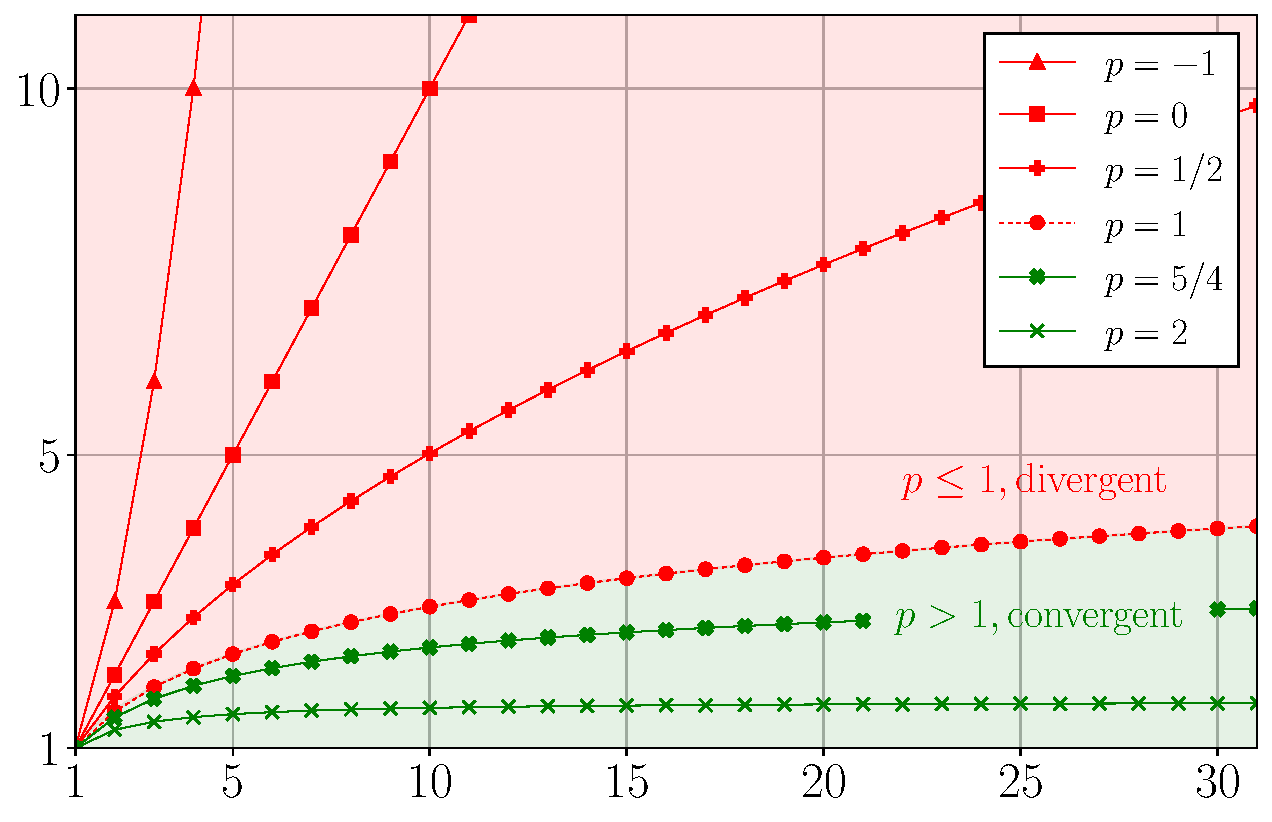
\includegraphics[width=0.83\textwidth]{UA_Figures/UA_ex2_7_5_fig.pdf}
        \caption{\( \sum_{n=1}^{\infty} \tfrac{1}{n^p} \) partial sums for various values of \( p \)}
        \label{fig:ex2.7.5}
    \end{figure}
\end{solution}

\begin{exercise}
\label{ex:2.7.6}
    Let's say that a series subverges if the sequence of partial sums contains a subsequence that converges. Consider this (invented) definition for a moment, and then decide which of the following statements are valid propositions about subvergent series:
    \begin{enumerate}
        \item If \( (a_n) \) is bounded, then \( \sum a_n \) subverges.

        \item All convergent series are subvergent.

        \item If \( \sum \abs{a_n} \) subverges, then \( \sum a_n \) subverges as well.

        \item If \( \sum a_n \) subverges, then \( (a_n) \) has a convergent subsequence.
    \end{enumerate}
\end{exercise}

\begin{solution}
    \begin{enumerate}
        \item This is false in general. For the bounded sequence \( (a_n) = (1, 1, 1, \ldots) \), the sequence of partial sums for the series \( \sum_{n=1}^{\infty} a_n \) is \( (1, 2, 3, \ldots) \). This sequence is unbounded and monotone and hence contains no convergent subsequence (\Cref{lem:ex2.6.2}).

        \item This is true. If the sequence of partial sums \( (s_n) \) is convergent then any subsequence of \( (s_n) \) is convergent; \( (s_n) \) itself, for example.

        \item This is true; we will prove the contrapositive statement. Define the sequences of partial sums
        \[
            s_n = \abs{a_1} + \cdots + \abs{a_n} \quad \text{and} \quad t_n = a_1 + \cdots + a_n.
        \]
        We want to show that if \( (t_n) \) has no convergent subsequence, then neither does \( (s_n) \). By the Bolzano-Weierstrass Theorem (Theorem 2.5.5) it must be the case that \( (t_n) \) is unbounded and, since \( t_n \leq s_n \) for all \( n \in \N \), it follows that \( (s_n) \) is unbounded. Thus \( (s_n) \) is an increasing unbounded sequence; such sequences do not have convergent subsequences, as shown in \Cref{lem:ex2.6.2}.

        \item This is false in general. Consider the sequence \( (a_n) = (1, -1, 2, -2, 3, -3, \ldots) \). The sequence of partial sums is \( (s_n) = (1, 0, 2, 0, 3, 0, \ldots) \), which has the convergent subsequence \( (0, 0, 0, \ldots) \); it follows that \( \sum_{n=1}^{\infty} a_n \) subverges. However, \( (a_n) \) has no convergent subsequence. To see this, observe that for any sequence \( (x_n) \) we have
        \[
            (x_n) \text{ has a convergent subsequence} \implies (\abs{x_n}) \text{ has a convergent subsequence},
        \]
        since if \( \lim_k x_{n_k} = x \) then \( \lim_k \abs{x_{n_k}} = \abs{x} \) (\Cref{ex:2.3.10} (b)). Because \( (\abs{a_n}) = (1, 1, 2, 2, 3, 3, \ldots) \) has no convergent subsequence (see \Cref{lem:ex2.6.2}), it follows that \( (a_n) \) has no convergent subsequence.
    \end{enumerate}
\end{solution}

\begin{exercise}
\label{ex:2.7.7}
    \begin{enumerate}
        \item Show that if \( a_n > 0 \) and \( \lim (n a_n) = l \) with \( l \neq 0 \), then the series \( \sum a_n \) diverges.

        \item Assume \( a_n > 0 \) and \( \lim (n^2 a_n) \) exists. Show that \( \sum a_n \) converges.
    \end{enumerate}
\end{exercise}

\begin{solution}
    The condition that \( a_n > 0 \) can be relaxed to \( a_n \geq 0 \) for both parts of this exercise.
    \begin{enumerate}
        \item Because \( n a_n \geq 0 \) for all \( n \in \N \), the Order Limit Theorem (Theorem 2.3.4) and the assumption \( l \neq 0 \) imply that \( l > 0 \). Since \( n a_n \to l \), there exists an \( N \in \N \) such that
        \[
            n \geq N \implies 0 < \frac{l}{2} < n a_n \implies 0 < \frac{l}{2 n} < a_n.
        \]
        Thus the series \( \sum_{n=1}^{\infty} a_n \) diverges by comparison (Theorem 2.7.4) with the divergent series \( \sum_{n=1}^{\infty} \tfrac{l}{2n} \) (Example 2.4.5).

        \item Suppose that \( \lim (n^2 a_n) = L \); the Order Limit Theorem (Theorem 2.3.4) implies that \( L \geq 0 \). There is an \( N \in \N \) such that
        \[
            n \geq N \implies 0 \leq n^2 a_n < L + 1 \implies 0 \leq a_n < \frac{L + 1}{n^2}.
        \]
        Since the series \( \sum_{n=1}^{\infty} \tfrac{L + 1}{n^2} \) is convergent (Corollary 2.4.7), the Comparison Test (Theorem 2.7.4) implies that \( \sum_{n=1}^{\infty} a_n \) is also convergent.
    \end{enumerate}
\end{solution}

\begin{exercise}
\label{ex:2.7.8}
    Consider each of the following propositions. Provide short proofs for those that are true and counterexamples for any that are not.
    \begin{enumerate}
        \item If \( \sum a_n \) converges absolutely, then \( \sum a_n^2 \) also converges absolutely.

        \item If \( \sum a_n \) converges and \( (b_n) \) converges, then \( \sum a_n b_n \) converges.

        \item If \( \sum a_n \) converges conditionally, then \( \sum n^2 a_n \) diverges.
    \end{enumerate}
\end{exercise}

\begin{solution}
    \begin{enumerate}
        \item This is true. Since the series \( \sum_{n=1}^{\infty} \abs{a_n} \) converges, we must have \( \lim \abs{a_n} = 0 \) (Theorem 2.7.3). There is then an \( N \in \N \) such that \( 0 \leq \abs{a_n} \leq 1 \) for \( n \geq N \); it follows that \( 0 \leq \abs{a_n}^2 = a_n^2 \leq \abs{a_n} \) for \( n \geq N \). We may now apply the Comparison Test (Theorem 2.7.4) to conclude that \( \sum_{n=1}^{\infty} a_n^2 \) converges absolutely.

        \item This is false. Let \( a_n = b_n = \tfrac{(-1)^n}{\sqrt{n}} \), so that \( \lim b_n = 0 \). Notice that \( \sum_{n=1}^{\infty} a_n \) converges by the Alternating Series Test (Theorem 2.7.7), but \( \sum_{n=1}^{\infty} a_n b_n = \sum_{n=1}^{\infty} \tfrac{1}{n} \), which is divergent (Example 2.4.5).

        \item This is true; we will prove that
        \[
            \sum_{n=1}^{\infty} \abs{a_n} \text{ diverges} \implies \sum_{n=1}^{\infty} n^2 a_n \text{ diverges},
        \]
        by proving the contrapositive statement
        \[
            \sum_{n=1}^{\infty} n^2 a_n \text{ converges} \implies \sum_{n=1}^{\infty} \abs{a_n} \text{ converges}.
        \]
        By Theorem 2.7.3 we have \( \lim(n^2 a_n) = 0 \), which implies that \( \lim(n^2 \abs{a_n}) = 0 \). We may now apply \Cref{ex:2.7.7} (b) to conclude that \( \sum_{n=1}^{\infty} \abs{a_n} \) is convergent.
    \end{enumerate}
\end{solution}

\begin{exercise}[Ratio Test]
\label{ex:2.7.9}
    Given a series \( \sum_{n=1}^{\infty} a_n \) with \( a_n \neq 0 \), the Ratio Test states that if \( (a_n) \) satisfies
    \[
        \lim \abs{\frac{a_{n+1}}{a_n}} = r < 1,
    \]
    then the series converges absolutely.
    \begin{enumerate}
        \item Let \( r' \) satisfy \( r < r' < 1 \). Explain why there exists an \( N \) such that \( n \geq N \) implies \( \abs{a_{n+1}} \leq \abs{a_n} r' \).

        \item Why does \( \abs{a_N} \sum (r')^n \) converge?

        \item Now, show that \( \sum \abs{a_n} \) converges, and conclude that \( \sum a_n \) converges.
    \end{enumerate}
\end{exercise}

\begin{solution}
    \begin{enumerate}
        \item Since \( \lim \abs{\frac{a_{n+1}}{a_n}} = r \) and \( r' - r > 0 \), there is an \( N \in \N \) such that
        \[
            n \geq N \implies \abs{\abs{\frac{a_{n+1}}{a_n}} - r} < r' - r \implies \frac{\abs{a_{n+1}}}{\abs{a_n}} < r' \implies \abs{a_{n+1}} < \abs{a_n} r'.
        \]

        \item Since \( 0 < r' < 1 \), the geometric series \( \sum_{n=0}^{\infty} (r')^n \) converges (Example 2.7.5).

        \item By part (a) we have
        \[
            \abs{a_{N+n}} < \abs{a_{N+n-1}} r' < \abs{a_{N+n-2}} (r')^2 < \cdots < \abs{a_N} (r')^n
        \]
        for any \( n \in \N \). It then follows from part (b) and the Comparison Test (Theorem 2.7.4) that the series
        \[
            \sum_{n=0}^{\infty} \abs{a_{N+n}} = \sum_{n=N}^{\infty} \abs{a_n}
        \]
        is convergent. Since a finite number of terms do not affect convergence, we see that the series \( \sum_{n=1}^{\infty} \abs{a_n} \) is convergent; the convergence of \( \sum_{n=1}^{\infty} a_n \) is then given by Theorem 2.7.6.
    \end{enumerate}
\end{solution}

\begin{exercise}[Infinite Products]
\label{ex:2.7.10}
    Review \Cref{ex:2.4.10} about infinite products and then answer the following questions:
    \begin{enumerate}
        \item Does \( \tfrac{2}{1} \cdot \tfrac{3}{2} \cdot \tfrac{5}{4} \cdot \tfrac{9}{8} \cdot \tfrac{17}{16} \cdots \) converge?

        \item The infinite product \( \tfrac{1}{2} \cdot \tfrac{3}{4} \cdot \tfrac{5}{6} \cdot \tfrac{7}{8} \cdot \tfrac{9}{10} \cdots \) certainly converges. (Why?) Does it converge to zero?

        \item In 1655, John Wallis famously derived the formula
        \[
            \paren{ \frac{2 \cdot 2}{1 \cdot 3} } \paren{ \frac{4 \cdot 4}{3 \cdot 5} } \paren{ \frac{6 \cdot 6}{5 \cdot 7} } \paren{ \frac{8 \cdot 8}{7 \cdot 9} } \cdots = \frac{\pi}{2}.
        \]
        Show that the left side of this identity at least converges to something. (A complete proof of this result is taken up in Section 8.3.)
    \end{enumerate}
\end{exercise}

\begin{solution}
    \begin{enumerate}
        \item This is the infinite product
        \[
            \prod_{n=0}^{\infty} \frac{2^n + 1}{2^n} = \prod_{n=0}^{\infty} \paren{ 1 + \frac{1}{2^n} }.
        \]
        By \Cref{ex:2.4.10}, this infinite product converges if and only if the series \( \sum_{n=0}^{\infty} \tfrac{1}{2^n} \) converges. This series is geometric with common ratio \( r = \tfrac{1}{2} \) and hence convergent by Example 2.7.5; it follows that the infinite product converges.

        \item This is the infinite product
        \[
            \prod_{n=1}^{\infty} \frac{2n - 1}{2n} = \prod_{n=1}^{\infty} \paren{ 1 - \frac{1}{2n} }.
        \]
        The sequence of partial products is positive and decreasing, since each term in the partial product satisfies \(0 < 1 - \tfrac{1}{2n} < 1 \); the Monotone Convergence Theorem (Theorem 2.4.2) then implies that the infinite product converges.

        Indeed, this infinite product converges to zero. To see this, let \( (p_m) \) be the sequence of partial products:
        \[
            p_m = \frac{1}{2} \cdot \frac{3}{4} \cdots \frac{2m - 1}{2m}.
        \]
        As stated above, \( (p_m) \) is decreasing and satisfies \( 0 < p_m < 1 \) for all \( m \in \N \), so we can look at the sequence of reciprocals \( \paren{ p_m^{-1} } \):
        \begin{align*}
            \frac{1}{p_m} &= \frac{2}{1} \cdot \frac{4}{3} \cdots \frac{2m}{2m - 1} \\[2mm]
            &= \paren{ 1 + \frac{1}{1} } \paren{ 1 + \frac{1}{3} } \cdots \paren{ 1 + \frac{1}{2m - 1} } \\[2mm]
            &\geq \sum_{n=1}^m \frac{1}{2n - 1} \\[2mm]
            &\geq \frac{1}{2} \sum_{n=1}^m \frac{1}{n}.
        \end{align*}
        It follows from Example 2.4.5 that \( \paren{ p_m^{-1} } \) is unbounded above. Thus, for any \( \epsilon > 0 \), there is an \( M \in \N \) such that \( p_M^{-1} > \epsilon^{-1} \), and since \( (p_m) \) is decreasing we then have
        \[
            m \geq M \implies \abs{p_m} = p_m \leq p_M < \epsilon.
        \]
        Hence \( \lim p_m = 0 \).

        \item This is the infinite product
        \[
            \prod_{n=1}^{\infty} \frac{(2n)^2}{(2n - 1)(2n + 1)} = \prod_{n=1}^{\infty} \paren{ 1 + \frac{1}{(2n - 1)(2n + 1)} } = \prod_{n=1}^{\infty} \paren{ 1 + \frac{1}{4n^2 - 1} }.
        \]
        By \Cref{ex:2.4.10}, this infinite product converges if and only if the series \( \sum_{n=0}^{\infty} \tfrac{1}{4n^2 - 1} \) converges. Observe that for all \( n \in \N \) we have
        \[
            n^2 - 1 \geq 0 \implies 4 n^2 - 1 \geq 3 n^2 \implies \frac{1}{4 n^2 - 1} \leq \frac{1}{3 n^2}.
        \]
        The series \( \sum_{n=1}^{\infty} \tfrac{1}{3 n^2} \) is convergent (Corollary 2.4.7), so the Comparison Test (Theorem 2.7.4) implies that the series \( \sum_{n=0}^{\infty} \tfrac{1}{4n^2 - 1} \) is also convergent; it follows that the infinite product
        \[
            \paren{ \frac{2 \cdot 2}{1 \cdot 3} } \paren{ \frac{4 \cdot 4}{3 \cdot 5} } \paren{ \frac{6 \cdot 6}{5 \cdot 7} } \paren{ \frac{8 \cdot 8}{7 \cdot 9} } \cdots
        \]
        converges.
    \end{enumerate}
    \begin{figure}
        \centering
        \begin{subfigure}{0.9\textwidth}
            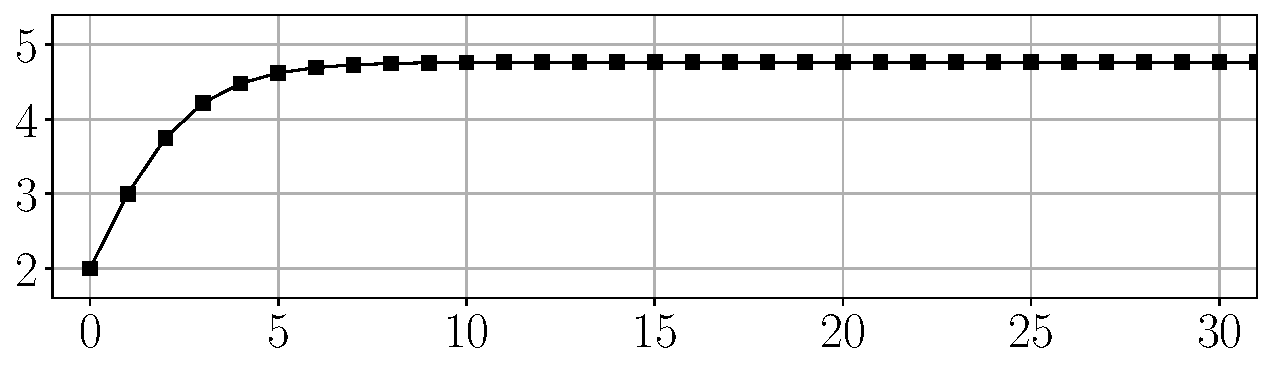
\includegraphics[width=\textwidth]{UA_Figures/UA_ex2_7_10_fig_a.pdf}
            \caption{\( \prod_{n=0}^m \paren{ 1 + \frac{1}{2^n} } \) for \( 0 \leq m \leq 30 \)}
        \end{subfigure} \\
        \begin{subfigure}{0.9\textwidth}
            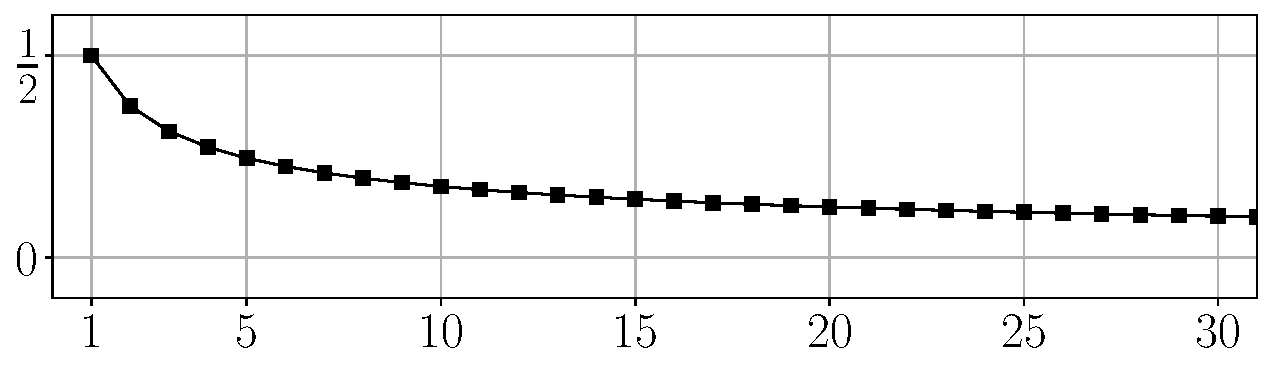
\includegraphics[width=\textwidth]{UA_Figures/UA_ex2_7_10_fig_b.pdf}
            \caption{\( \prod_{n=1}^m \paren{ 1 - \frac{1}{2n} } \) for \( 1 \leq m \leq 30 \)}
        \end{subfigure} \\
        \begin{subfigure}{0.9\textwidth}
            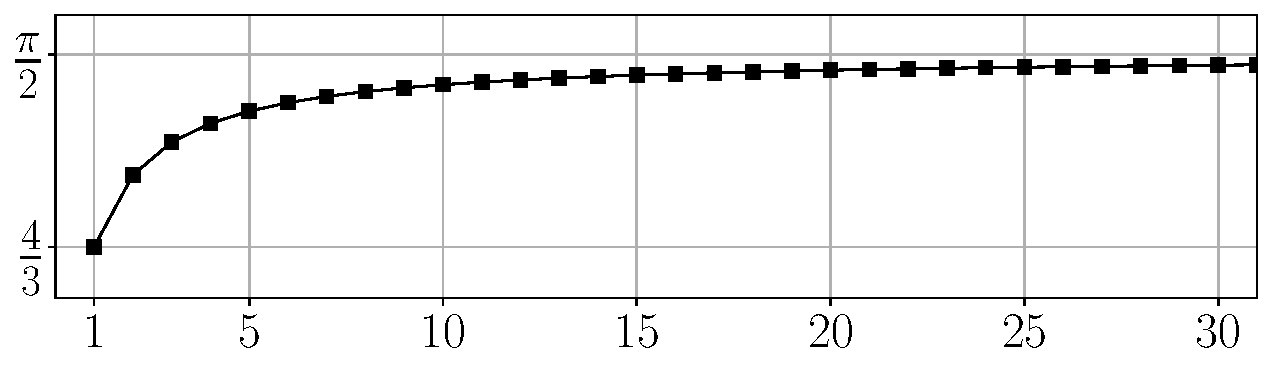
\includegraphics[width=\textwidth]{UA_Figures/UA_ex2_7_10_fig_c.pdf}
            \caption{\( \prod_{n=1}^m \paren{ 1 + \frac{1}{4n^2 - 1} } \) for \( 1 \leq m \leq 30 \)}
        \end{subfigure}
        \caption{\Cref{ex:2.7.10} partial products}
    \end{figure}
\end{solution}

\begin{exercise}
\label{ex:2.7.11}
    Find examples of two series \( \sum a_n \) and \( \sum b_n \) both of which diverge but for which \( \sum \min \{ a_n, b_n \} \) converges. To make it more challenging, produce examples where \( (a_n) \) and \( (b_n) \) are strictly positive and decreasing.
\end{exercise}

\begin{solution}
    Consider the series
    \begin{gather*}
        \sum_{n=1}^{\infty} a_n = \underbrace{\frac{1}{1^2}}_{\substack{1 \text{ term} \\ \text{sum = } 1}} + \frac{1}{2^2} + \cdots + \frac{1}{5^2} +  \underbrace{\frac{1}{6^2} + \cdots + \frac{1}{6^2}}_{\substack{6^2 \text{ terms} \\ \text{sum = } 1}} + \frac{1}{42^2} + \cdots + \frac{1}{1805^2} + \cdots \\[4mm]
        \sum_{n=1}^{\infty} b_n = \frac{1}{1^2} + \underbrace{\frac{1}{2^2} + \cdots + \frac{1}{2^2}}_{\substack{2^2 \text{ terms} \\ \text{sum = } 1}} + \frac{1}{6^2} + \cdots + \frac{1}{41^2} + \underbrace{\frac{1}{42^2} + \cdots + \frac{1}{42^2}}_{\substack{42^2 \text{ terms} \\ \text{sum = } 1}} + \cdots
    \end{gather*}
    Both \( (a_n) \) and \( (b_n) \) are strictly positive and decreasing and
    \[
        \sum_{n=1}^{\infty} \min \{ a_n, b_n \} = \sum_{n=1}^{\infty} \frac{1}{n^2},
    \]
    which is a convergent series. Furthermore, both \( \sum a_n \) and \( \sum b_n \) diverge since their respective sequences of partial sums are unbounded; we can find arbitrarily many groupings of terms which sum to 1 as shown above.
\end{solution}

\begin{exercise}[Summation by parts]
\label{ex:2.7.12}
    Let \( (x_n) \) and \( (y_n) \) be sequences, let \( s_n = x_1 + x_2 + \cdots + x_n \) and set \( s_0 = 0 \). Use the observation that \( x_j = s_j - s_{j-1} \) to verify the formula
    \[
        \sum_{j=m}^n x_j y_j = s_n y_{n+1} - s_{m-1} y_m + \sum_{j=m}^n s_j (y_j - y_{j+1}).
    \]
\end{exercise}

\begin{solution}
    For positive integers \( n > m \),
    \begin{align*}
        \sum_{j=m}^n x_j y_j &= \sum_{j=m}^n (s_j - s_{j-1}) y_j \\
        &= \sum_{j=m}^n s_j y_j - \sum_{j=m}^n s_{j-1} y_j \\
        &= \sum_{j=m}^n s_j y_j - \sum_{j=m-1}^{n-1} s_j y_{j+1} \\
        &= \sum_{j=m}^n s_j y_j - \sum_{j=m}^n s_j y_{j+1} + s_n y_{n+1} - s_{m-1} y_m \\
        &= s_n y_{n+1} - s_{m-1} y_m + \sum_{j=m}^n s_j (y_j - y_{j+1}).
    \end{align*}
\end{solution}

\begin{exercise}[Abel's Test]
\label{ex:2.7.13}
    Abel's Test for convergence states that if the series \( \sum_{k=1}^{\infty} x_k \) converges, and if \( (y_k) \) is a sequence satisfying
    \[
        y_1 \geq y_2 \geq y_3 \geq \cdots \geq 0,
    \]
    then the series \( \sum_{k=1}^{\infty} x_k y_k \) converges.
    \begin{enumerate}
        \item Use \Cref{ex:2.7.12} to show that
        \[
            \sum_{k=1}^n x_k y_k = s_n y_{n+1} + \sum_{k=1}^n s_k (y_k - y_{k+1}),
        \]
        where \( s_n = x_1 + x_2 + \cdots + x_n \).

        \item Use the Comparison Test to argue that \( \sum_{k=1}^{\infty} s_k (y_k - y_{k+1}) \) converges absolutely, and show how this leads directly to a proof of Abel's Test.
    \end{enumerate}
\end{exercise}

\begin{solution}
    \begin{enumerate}
        \item This follows immediately from \Cref{ex:2.7.12}, taking \( m = 1 \) and remembering that \( s_0 := 0 \).

        \item By assumption the sequence \( (s_k) \) is convergent and hence, by Theorem 2.3.2, bounded by some \( M > 0 \), so that for each \( k \in \N \) we have the inequality
        \[
            0 \leq \abs{s_k (y_k - y_{k+1})} = \abs{s_k} (y_k - y_{k+1}) \leq M (y_k - y_{k+1}). \tag{1}
        \]
        Notice that since \( (y_k) \) is decreasing and bounded below, the limit \( y := \lim_{k \to \infty} y_k \) exists by the Monotone Convergence Theorem (Theorem 2.4.2). It follows that the series \( \sum_{k=1}^{\infty} (y_k - y_{k+1}) \) is convergent since, letting \( t_m \) be the \( m \)\ts{th} partial sum, we have
        \[
            t_m = (y_1 - y_2) + (y_2 - y_3) + \cdots + (y_m - y_{m+1}) = y_1 - y_{m+1} \to y_1 - y \text{ as } m \to \infty.
        \]
        Inequality (1) and the Comparison Test (Theorem 2.7.4) then imply that \( \sum_{k=1}^{\infty} s_k(y_k - y_{k+1}) \) is absolutely convergent and hence convergent (Theorem 2.7.6). From part (a) we have \( \sum_{k=1}^n x_k y_k = s_n y_{n+1} + \sum_{k=1}^n s_k (y_k - y_{k+1}) \); it follows that
        \[
            \sum_{k=1}^{\infty} x_k y_k = \lim_{n \to \infty} \paren{ s_n y_{n+1} + \sum_{k=1}^n s_k (y_k - y_{k+1}) } = y \sum_{k=1}^{\infty} x_k + \sum_{k=1}^{\infty} s_k (y_k - y_{k+1}).
        \]
    \end{enumerate}
\end{solution}

\begin{exercise}[Dirichlet's Test]
\label{ex:2.7.14}
    Dirichlet's Test for convergence states that if the partial sums of \( \sum_{k=1}^{\infty} x_k \) are bounded (but not necessarily convergent), and if \( (y_k) \) is a sequence satisfying \( y_1 \geq y_2 \geq y_3 \geq \cdots \geq 0 \) with \( \lim y_k = 0 \), then the series \( \sum_{k=1}^{\infty} x_k y_k \) converges.
    \begin{enumerate}
        \item Point out how the hypothesis of Dirichlet's Test differs from that of Abel's Test in \Cref{ex:2.7.13}, but show that essentially the same strategy can be used to provide a proof.

        \item Show how the Alternating Series Test (Theorem 2.7.7) can be derived as a special case of Dirichlet's Test.
    \end{enumerate}
\end{exercise}

\begin{solution}
    \begin{enumerate}
        \item Abel's Test has the stronger hypothesis that the sequence of partial sums of \( \sum_{k=1}^{\infty} x_k \) is convergent (and hence bounded), but the weaker hypothesis that \( (y_k) \) only satisfies \( y_1 \geq y_2 \geq y_3 \geq \cdots \geq 0 \) without necessarily converging to zero.

        The proof of Dirichlet's Test is almost identical to the proof of Abel's Test given in \Cref{ex:2.7.13} (b). Letting \( (s_k) \) be the \( k \)\ts{th} partial sum of \( \sum_{n=1}^{\infty} x_n \), we are given that \( (s_k) \) is bounded by some \( M > 0 \). It follows that
        \[
            0 \leq \abs{s_k (y_k - y_{k+1})} = \abs{s_k} (y_k - y_{k+1}) \leq M (y_k - y_{k+1}) \tag{1}
        \]
        for each \( k \in \N \). The series \( \sum_{k=1}^{\infty} (y_k - y_{k+1}) \) is convergent since it has \( m \)\ts{th} partial sum
        \[
            (y_1 - y_2) + (y_2 - y_3) + \cdots + (y_m - y_{m+1}) = y_1 - y_{m+1} \to y_1 \text{ as } m \to \infty.
        \]
        Inequality (1) and the Comparison Test (Theorem 2.7.4) then imply that \( \sum_{k=1}^{\infty} s_k(y_k - y_{k+1}) \) is absolutely convergent and hence convergent. Since \( (s_k) \) is bounded and \( \lim y_k = 0 \), we have \( \lim (s_k y_{k+1}) = 0 \) also (\Cref{ex:2.3.9} (b)). It follows that
        \[
            \sum_{k=1}^{\infty} x_k y_k = \lim_{n \to \infty} \paren{ s_n y_{n+1} + \sum_{k=1}^n s_k (y_k - y_{k+1}) } = \sum_{k=1}^{\infty} s_k (y_k - y_{k+1}).
        \]

        \item The Alternating Series Test (Theorem 2.7.7) can be recovered from Dirichlet's Test by taking \( x_k = (-1)^{k+1} \); the sequence of partial sums of \( \sum_{k=1}^{\infty} x_k \) is then \( (1, 0, 1, 0, \ldots) \), which is certainly bounded.
    \end{enumerate}
\end{solution}

\section{Double Summations and Products of Infinite Series}
\label{sec:2.8}

\begin{exercise}
\label{ex:2.8.1}
    Using the particular array \( (a_{ij}) \) from Section 2.1, compute \( \lim_{n \to \infty} s_{nn} \). How does this value compare to the two iterated values for the sum already computed?
\end{exercise}

\begin{solution}
    The array in question is
    \[
        \begin{bmatrix}
            -1 & \tfrac{1}{2} & \tfrac{1}{4} & \tfrac{1}{8} & \tfrac{1}{16} & \cdots \\[3mm]
            0 & -1 & \tfrac{1}{2} & \tfrac{1}{4} & \tfrac{1}{8} & \cdots \\[3mm]
            0 & 0 & -1 & \tfrac{1}{2} & \tfrac{1}{4} & \cdots \\[3mm]
            0 & 0 & 0 & -1 & \tfrac{1}{2} & \cdots \\[3mm]
            0 & 0 & 0 & 0 & -1 & \cdots \\[1mm]
            \vdots & \vdots & \vdots & \vdots & \vdots & \ddots
        \end{bmatrix},
    \]
    where \( a_{ij} = 2^{i-j} \) if \( j > i, a_{ij} = -1 \) if \( j = i \), and \( a_{ij} = 0 \) if \( j < i \). If we let \( f(j) \) be the sum of the first row up to the \( j \)\ts{th} column, then using the formula for the partial sums of a geometric series, we find that
    \begin{align*}
        f(j) &= \begin{cases}
            -1 & \text{if } j = 1, \\
            -1 + \tfrac{1}{2} + \cdots + \tfrac{1}{2^{j-1}} = -\tfrac{1}{2^{j-1}} & \text{if } j \geq 2
        \end{cases} \\[2mm]
        &= -\frac{1}{2^{j-1}}.
    \end{align*}
    Since subsequent rows are simply the first row shifted along, it is clear that \( s_{11} = f(1), s_{22} = f(1) + f(2), s_{33} = f(1) + f(2) + f(3) \), and in general
    \[
        s_{nn} = \sum_{j=1}^n f(j) = \sum_{j=1}^n \frac{-1}{2^{j-1}} = -\sum_{j=0}^{n-1} \frac{1}{2^j}.
    \]
    It follows that
    \[
        \lim_{n \to \infty} s_{nn} = -\sum_{j=0}^{\infty} \frac{1}{2^j} = -2.
    \]
    At the beginning of Section 2.1, we found that summing along the rows first gave a value of 0 for the double sum, whereas summing down the columns first gave a value of \( -2 \).
\end{solution}

\begin{exercise}
\label{ex:2.8.2}
    Show that if the iterated series
    \[
        \sum_{i=1}^{\infty} \sum_{j=1}^{\infty} \abs{a_{ij}}
    \]
    converges (meaning for each fixed \( i \in \N \) the series \( \sum_{j=1}^{\infty} \abs{a_{ij}} \) converges to some real number \( b_i \), and the series \( \sum_{i=1}^{\infty} b_i \) converges as well), then the iterated series
    \[
        \sum_{i=1}^{\infty} \sum_{j=1}^{\infty} a_{ij}
    \]
    converges.
\end{exercise}

\begin{solution}
    For each \( i \in \N \), Theorem 2.7.6 implies that the series \( \sum_{j=1}^{\infty} a_{ij} \) converges to some real number \( c_i \). Observe that
    \[
        0 \leq \abs{c_i} = \abs{\sum_{j=1}^{\infty} a_{ij}} \leq \sum_{j=1}^{\infty} \abs{a_{ij}} = b_i.
    \]
    Since \( \sum_{i=1}^{\infty} b_i \) converges, the Comparison Test (Theorem 2.7.4) implies that the series \( \sum_{i=1}^{\infty} c_i \) is absolutely convergent and hence convergent (Theorem 2.7.6).
\end{solution}

\begin{exercise}
\label{ex:2.8.3}
        \begin{enumerate}
        \item Prove that \( (t_{nn}) \) converges.

        \item Now, use the fact that \( (t_{nn}) \) is a Cauchy sequence to argue that \( (s_{nn}) \) converges.
    \end{enumerate}
\end{exercise}

\begin{solution}
    \begin{enumerate}
        \item Since \( \abs{a_{ij}} \geq 0 \) for all positive integers \( i \) and \( j \), the sequence \( (t_{nn}) \) is increasing and bounded above by the real number \( \sum_{i=1}^{\infty} \sum_{j=1}^{\infty} \abs{a_{ij}} \). Thus \( (t_{nn}) \) converges by the Monotone Convergence Theorem (Theorem 2.4.2).

        \item Suppose \( n > m \) are positive integers. By examining the following array, which has the special case \( n = 6 \) and \( m = 3 \),
        \begin{center}
            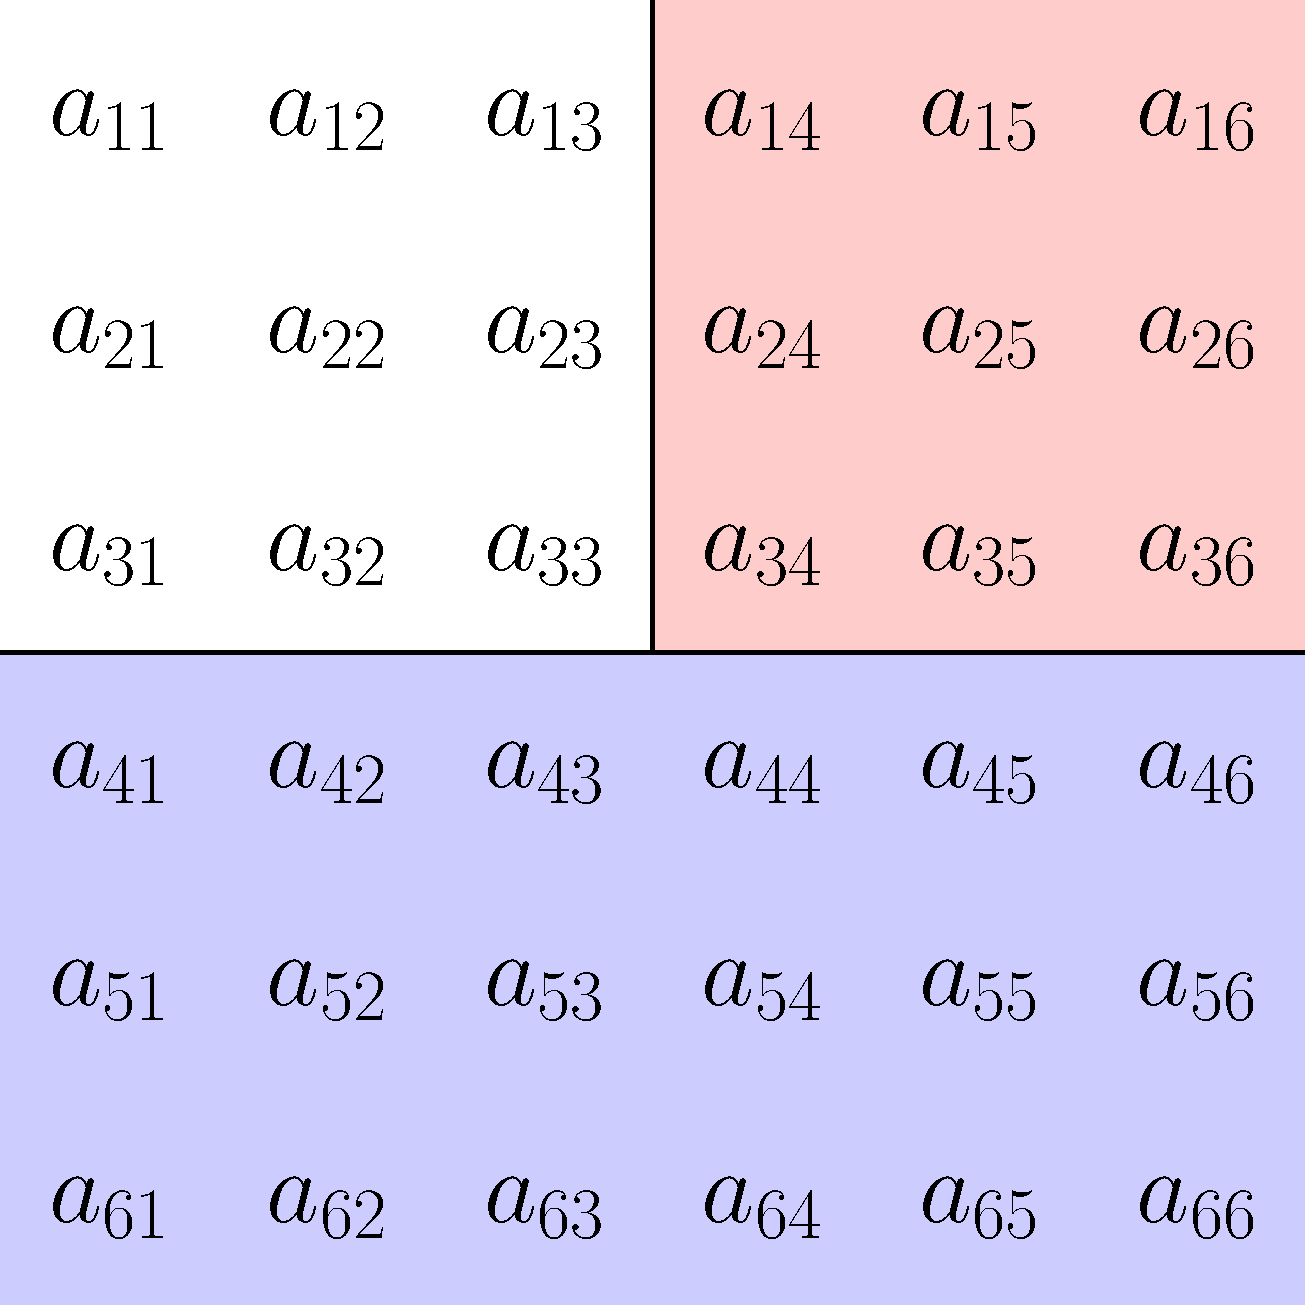
\includegraphics[width=0.4\textwidth]{UA_Figures/UA_ex2_8_3_fig.pdf}
        \end{center}
        we see that
        \[
            \sum_{i=1}^n \sum_{j=1}^n a_{ij} - \sum_{i=1}^m \sum_{j=1}^m a_{ij} = \textcolor{red}{\sum_{i=1}^m \sum_{j=m+1}^n a_{ij}} + \textcolor{blue}{\sum_{i=m+1}^n \sum_{j=1}^n a_{ij}}.
        \]
        (The sum of the top right ``square'' (in red) and the bottom ``rectangle'' (in blue) of the array.) Let \( \epsilon > 0 \) be given. Since \( (t_{nn}) \) is a Cauchy sequence, there exists an \( N \in \N \) such that \( n > m \geq N \) implies
        \[
            \abs{t_{nn} - t_{mm}} = t_{nn} - t_{mm} < \epsilon.
        \]
        For such \( n \) and \( m \), observe that
        \begin{align*}
            \abs{s_{nn} - s_{mm}} &= \abs{\sum_{i=1}^n \sum_{j=1}^n a_{ij} - \sum_{i=1}^m \sum_{j=1}^m a_{ij}} \\[2mm]
            &= \abs{\sum_{i=1}^m \sum_{j=m+1}^n a_{ij} + \sum_{i=m+1}^n \sum_{j=1}^n a_{ij}} \\[2mm]
            &\leq \sum_{i=1}^m \sum_{j=m+1}^n \abs{a_{ij}} + \sum_{i=m+1}^n \sum_{j=1}^n \abs{a_{ij}} \\
            &= t_{nn} - t_{mm} \\
            &< \epsilon.
        \end{align*}
        It follows that \( (s_{nn}) \) is a Cauchy sequence and hence convergent.
    \end{enumerate}
\end{solution}

\begin{exercise}
\label{ex:2.8.4}
    \begin{enumerate}
        \item Let \( \epsilon > 0 \) be arbitrary and argue that there exists an \( N_1 \in \N \) such that \( m, n \geq N_1 \) implies \( B - \tfrac{\epsilon}{2} < t_{mn} \leq B \).

        \item Now, show that there exists an \( N \) such that
        \[
            \abs{s_{mn} - S} < \epsilon
        \]
        for all \( m, n \geq N \).
    \end{enumerate}
\end{exercise}

\begin{solution}
    \begin{enumerate}
        \item By Lemma 1.3.8, there exist positive integers \( m', n' \) such that \( B - \tfrac{\epsilon}{2} < t_{m' n'} \leq B \). Set \( N_1 = \max \{ m', n' \} \). Since each \( \abs{a_{ij}} \) is positive, \( (t_{mn}) \) is increasing in both \( m \) and \( n \); it follows that for \( m, n \geq N_1 \) we have \( B - \tfrac{\epsilon}{2} < t_{mn} \leq B \).

        \item Since \( \lim_{n \to \infty} s_{nn} = S \), there is an \( N_2 \in \N \) such that \( \abs{s_{nn} - S} < \frac{\epsilon}{2} \) for all \( n \geq N_2 \). Set \( N = \max \{ N_1, N_2 \} \) and suppose that \( m, n > N \). Similarly to \Cref{ex:2.8.3} (b), we have
        \begin{align*}
            \abs{s_{mn} - s_{NN}} &= \abs{\sum_{i=1}^m \sum_{j=1}^n a_{ij} - \sum_{i=1}^N \sum_{j=1}^N a_{ij}} \\[2mm]
            &= \abs{\sum_{i=1}^N \sum_{j=N+1}^n a_{ij} + \sum_{i=N+1}^m \sum_{j=1}^n a_{ij}} \\[2mm]
            &\leq \sum_{i=1}^N \sum_{j=N+1}^n \abs{a_{ij}} + \sum_{i=N+1}^m \sum_{j=1}^n \abs{a_{ij}} \\
            &= t_{mn} - t_{NN} \\
            &\leq B - t_{NN} \\
            &< \frac{\epsilon}{2}.
        \end{align*}
        It follows that
        \[
            \abs{s_{mn} - S} \leq \abs{s_{mn} - s_{NN}} + \abs{s_{NN} - S} < \frac{\epsilon}{2} + \frac{\epsilon}{2} = \epsilon.
        \]
    \end{enumerate}
\end{solution}

\begin{exercise}
\label{ex:2.8.5}
    \begin{enumerate}
        \item Show that for all \( m \geq N \)
        \[
            \abs{(r_1 + r_2 + \cdots + r_m) - S} \leq \epsilon.
        \]
        Conclude that the iterated sum \( \sum_{i=1}^{\infty} \sum_{j=1}^{\infty} a_{ij} \) converges to \( S \).

        \item Finish the proof by showing that the other iterated sum, \( \sum_{j=1}^{\infty} \sum_{i=1}^{\infty} a_{ij} \), converges to \( S \) as well. Notice that the same argument can be used once it is established that, for each fixed column \( j \), the sum \( \sum_{i=1}^{\infty} a_{ij} \) converges to some real number \( c_j \).
    \end{enumerate}
\end{exercise}

\begin{solution}
    \begin{enumerate}
        \item Suppose that \( n \geq N \). Then
        \begin{align*}
            \abs{(r_1 + \cdots + r_m) - S} &\leq \abs{(r_1 + \cdots + r_m) - s_{mn}} + \abs{s_{mn} - S} \\[2mm]
            &< \abs{(r_1 + \cdots + r_m) - \paren{ \sum_{j=1}^n a_{1j} + \cdots + \sum_{j=1}^n a_{mj} }} + \epsilon \\[2mm]
            &\leq \abs{r_1 - \sum_{j=1}^n a_{1j}} + \cdots + \abs{r_m - \sum_{j=1}^n a_{mj}} + \epsilon.
        \end{align*}
        Since this is true for any \( n \geq N \) and for any given \( i \) we have \( \sum_{j=1}^{\infty} a_{ij} = r_i \), taking the limit in \( n \) on both sides of the inequality
        \[
            \abs{(r_1 + r_2 + \cdots + r_m) - S} < \abs{r_1 - \sum_{j=1}^n a_{1j}} + \abs{r_2 - \sum_{j=1}^n a_{2j}} + \cdots + \abs{r_m - \sum_{j=1}^n a_{mj}} + \epsilon
        \]
        gives us
        \[
            \abs{(r_1 + r_2 + \cdots + r_m) - S} \leq \epsilon.
        \]
        It follows that \( \lim_{m \to \infty} \paren{ \sum_{i=1}^m r_i } = S \), i.e., \( \sum_{i=1}^{\infty} \sum_{j=1}^{\infty} a_{ij} = S \).

        \item Fix \( j \in \N \) and let \( (x_n) \) be the sequence of partial sums of the series \( \sum_{i=1}^{\infty} \abs{a_{ij}} \), i.e.,
        \[
            x_n = \abs{a_{1j}} + \abs{a_{2j}} + \cdots + \abs{a_{nj}}.
        \]
        Since each \( \abs{a_{ij}} \) is a term of the convergent series \( \sum_{j=1}^{\infty} \abs{a_{ij}} = r_i \), which has only non-negative terms, we see that \( \abs{a_{ij}} \leq r_i \), so that
        \[
            x_n \leq r_1 + r_2 + \cdots + r_n \leq \sum_{i=1}^{\infty} r_i,
        \]
        where the last inequality follows since each \( r_i \) is non-negative. So \( (x_n) \) is an increasing and bounded sequence and hence converges by the Monotone Convergence Theorem (Theorem 2.4.2). It follows that \( \sum_{i=1}^{\infty} a_{ij} \) converges to some (non-negative) real number \( c_j \).

        Let \( \epsilon > 0 \) be given. As in \Cref{ex:2.8.4}, there is an \( N \in \N \) such that \( \abs{s_{mn} - S} < \epsilon \) for all \( m, n \geq N \). We can write \( s_{mn} \) as
        \[
            s_{mn} = \sum_{i=1}^m a_{i1} + \sum_{i=1}^m a_{i2} + \cdots + \sum_{i=1}^m a_{in}.
        \]
        Suppose that \( m, n \geq N \). Then
        \begin{align*}
            \abs{(c_1 + \cdots + c_n) - S} &\leq \abs{(c_1 + \cdots + c_n) - s_{mn}} + \abs{s_{mn} - S} \\[2mm]
            &< \abs{(c_1 + \cdots + c_n) - \paren{ \sum_{i=1}^m a_{i1} + \cdots + \sum_{i=1}^m a_{in} }} + \epsilon \\[2mm]
            &\leq \abs{c_1 - \sum_{i=1}^m a_{i1}} + \cdots + \abs{c_n - \sum_{i=1}^m a_{in}} + \epsilon.
        \end{align*}
        Since this is true for any \( m \geq N \) and for any given \( j \) we have \( \sum_{i=1}^{\infty} a_{ij} = c_j \), taking the limit in \( m \) on both sides of the inequality
        \[
            \abs{(c_1 + c_2 + \cdots + c_n) - S} < \abs{c_1 - \sum_{i=1}^m a_{i1}} + \abs{c_2 - \sum_{i=1}^m a_{i2}} + \cdots + \abs{c_n - \sum_{i=1}^m a_{in}} + \epsilon
        \]
        gives us
        \[
            \abs{(c_1 + c_2 + \cdots + c_n) - S} \leq \epsilon.
        \]
        It follows that \( \lim_{n \to \infty} \paren{ \sum_{j=1}^n c_j } = S \), i.e., \( \sum_{j=1}^{\infty} \sum_{i=1}^{\infty} a_{ij} = S \).
    \end{enumerate}
\end{solution}

\begin{exercise}
\label{ex:2.8.6}
    \begin{enumerate}
        \item Assuming the hypothesis---and hence the conclusion---of Theorem 2.8.1, show that \( \sum_{k=2}^{\infty} d_k \) converges absolutely.

        \item Imitate the strategy in the proof of Theorem 2.8.1 to show that \( \sum_{k=2}^{\infty} d_k \) converges to \( S = \lim_{n \to \infty} s_{nn} \).
    \end{enumerate}
\end{exercise}

\begin{solution}
    \begin{enumerate}
        \item Observe that
        \begin{gather*}
            \abs{d_2} = \abs{a_{11}} = \sum_{i=1}^1 \sum_{j=1}^{2-i} \abs{a_{ij}}, \\[1.25mm]
            \abs{d_2} + \abs{d_3} = \abs{a_{11}} + \abs{a_{12} + a_{21}} \leq (\abs{a_{11}} + \abs{a_{12}}) + \abs{a_{21}} = \sum_{i=1}^2 \sum_{j=1}^{3-i} \abs{a_{ij}},
        \end{gather*}
        \vspace{-4mm}
        \begin{multline*}
            \abs{d_2} + \abs{d_3} + \abs{d_4} = \abs{a_{11}} + \abs{a_{12} + a_{21}} + \abs{a_{13} + a_{22} + a_{31}} \\[1.25mm]
            \leq (\abs{a_{11}} + \abs{a_{12}} + \abs{a_{13}}) + (\abs{a_{21}} + \abs{a_{22}}) + \abs{a_{31}} = \sum_{i=1}^3 \sum_{j=1}^{4-i} \abs{a_{ij}},
        \end{multline*}
        and in general for \( n \geq 2 \),
        \[
            \sum_{k=2}^n \abs{d_k} \leq \sum_{i=1}^{n-1} \sum_{j=1}^{n-i} \abs{a_{ij}} \leq \sum_{i=1}^{\infty} \sum_{j=1}^{\infty} \abs{a_{ij}},
        \]
        where the last inequality follows since each \( \abs{a_{ij}} \) is non-negative. By assumption \( \sum_{i=1}^{\infty} \) \( \sum_{j=1}^{\infty} \abs{a_{ij}} \) is finite, so the sequence \( \sum_{k=2}^n \abs{d_k} \) is increasing and bounded above and hence converges by the Monotone Convergence Theorem (Theorem 2.4.2).

        \item By considering \Cref{fig:ex2.8.6_1}, which shows the special case \( n = 6 \), we see that for each \( n \geq 2 \),
        \[
            s_{nn} - \sum_{k=2}^n d_k = \sum_{i=1}^n \sum_{j=n+1-i}^n a_{ij}.
        \]
        \begin{figure}[H]
            \centering
            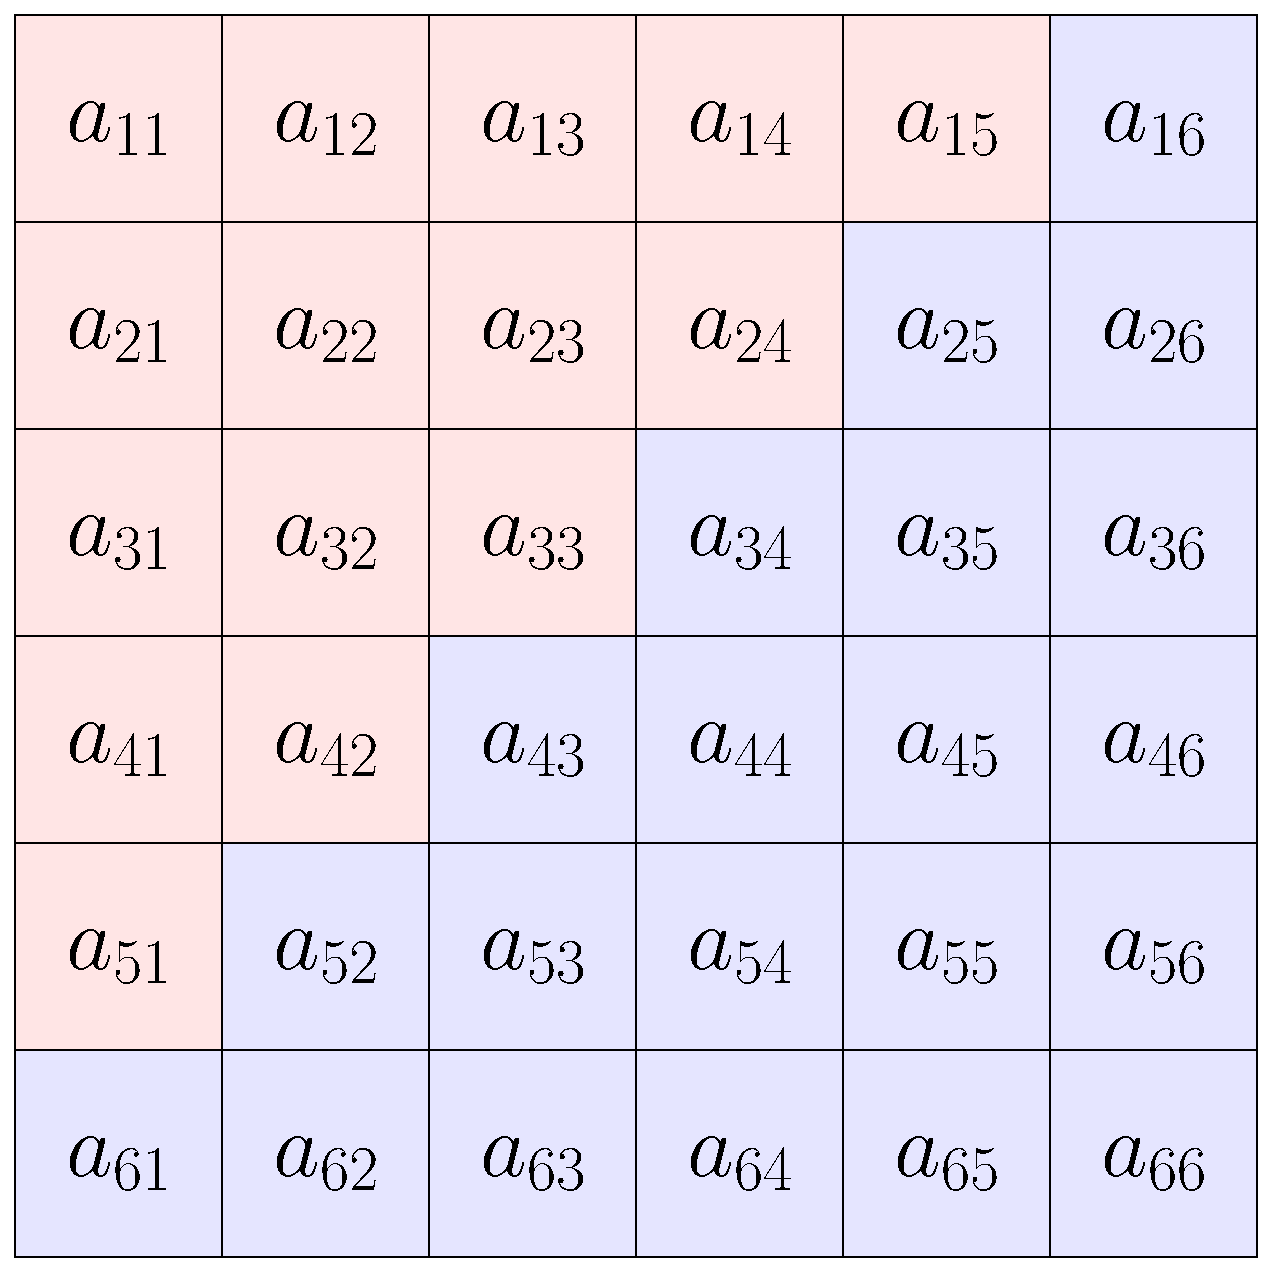
\includegraphics[width=0.5\textwidth]{UA_Figures/UA_ex2_8_6_fig_1.pdf}
            \caption{\( s_{66} - \textcolor{red}{\sum_{k=2}^6 d_k} = \textcolor{blue}{\sum_{i=1}^6 \sum_{j=7-i}^6 a_{ij}} \)}
            \label{fig:ex2.8.6_1}
        \end{figure}
        \noindent Similarly, letting
        \[
            e_k = \abs{a_{1,k-1}} + \abs{a_{2,k-2}} + \cdots + \abs{a_{k-1,1}}
        \]
        for \( k \geq 2 \), we find that
        \[
            t_{nn} - \sum_{k=2}^n e_k = \sum_{i=1}^n \sum_{j=n+1-i}^n \abs{a_{ij}}
        \]
        for each \( n \geq 2 \). It follows that
        \[
            \abs{s_{nn} - \sum_{k=2}^n d_k} = \abs{\sum_{i=1}^n \sum_{j=n+1-i}^n a_{ij}} \leq \sum_{i=1}^n \sum_{j=n+1-i}^n \abs{a_{ij}} = t_{nn} - \sum_{k=2}^n e_k. \tag{1}
        \]
        Let \( \epsilon > 0 \) be given. Since \( \lim_{n \to \infty} s_{nn} = S \) and \( (t_{nn}) \) is an increasing Cauchy sequence, there are positive integers \( N_1, N_2 \) such that
        \[
            n \geq N_1 \implies \abs{s_{nn} - S} < \frac{\epsilon}{2} \hspaceand n > m \geq N_2 \implies t_{nn} - t_{mm} < \frac{\epsilon}{2}. \tag{2}
        \]
        Set \( N = \max \{ N_1, 2 N_2 \} \) and suppose \( n \geq N \). Since \( n \geq 2 N_2 \), each term of \( t_{N_2 N_2} \) appears in \( \sum_{k=2}^n e_k \) (see \Cref{fig:ex2.8.6_2}, which has the special case \( n = 6 \) and \( N_2 = 3 \)).
        \begin{figure}[H]
            \centering
            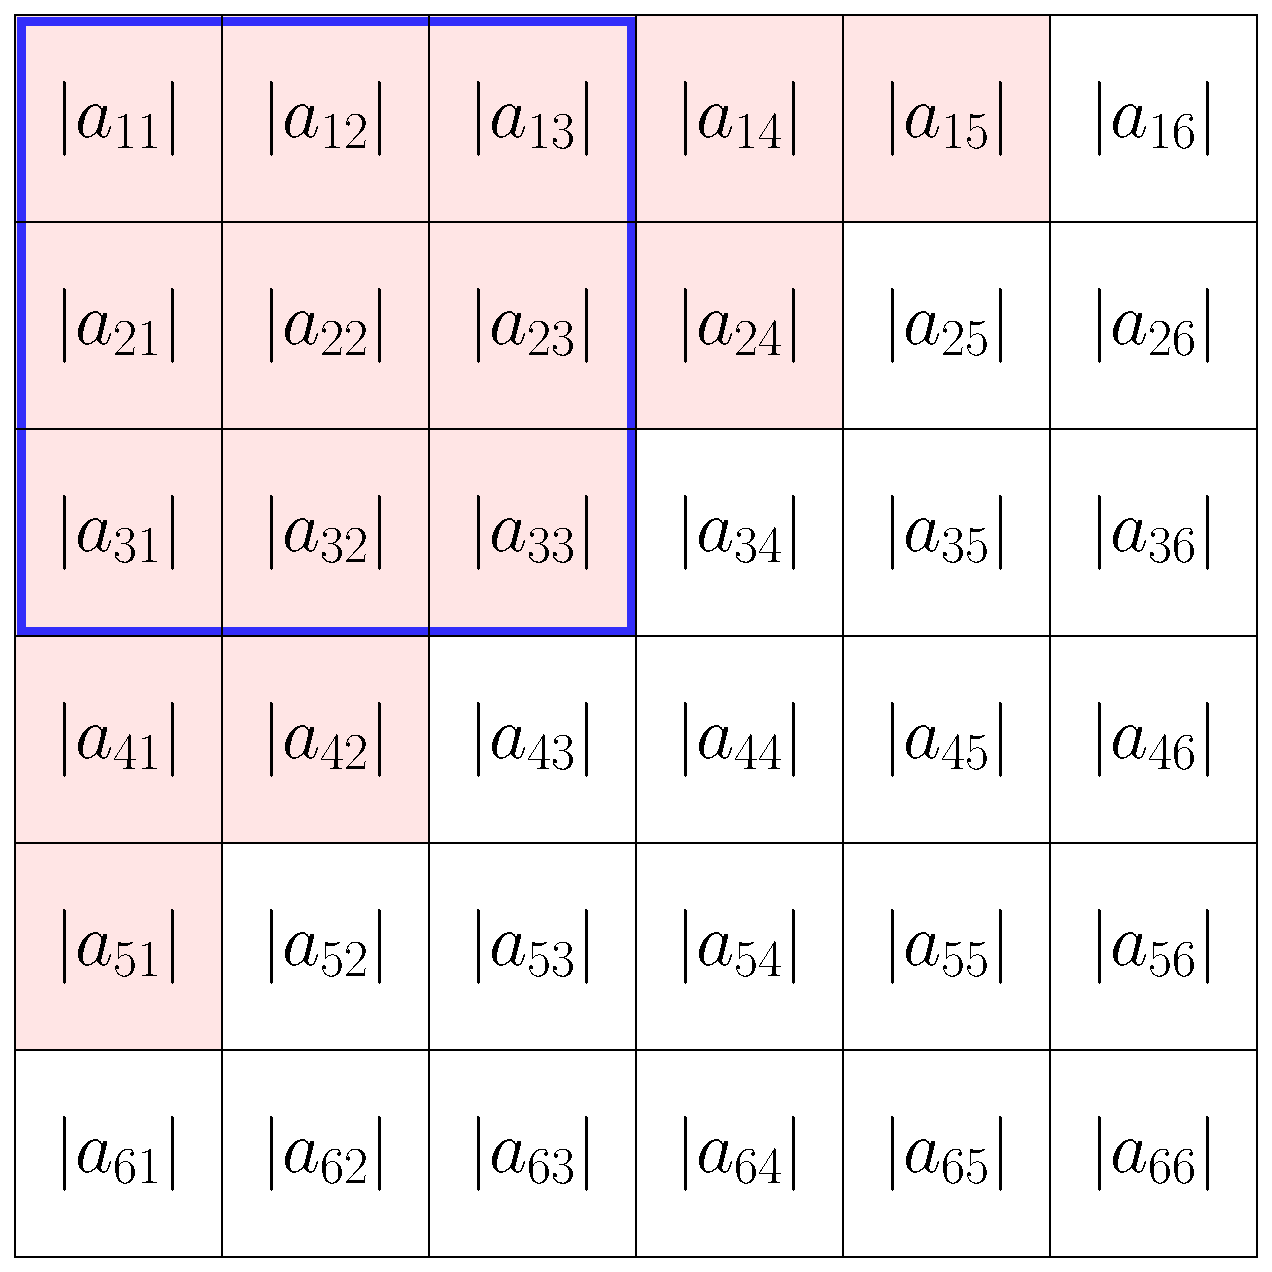
\includegraphics[width=0.5\textwidth]{UA_Figures/UA_ex2_8_6_fig_2.pdf}
            \caption{\( \textcolor{blue}{t_{33}} \leq \textcolor{red}{\sum_{k=2}^6 e_k} \)}
            \label{fig:ex2.8.6_2}
        \end{figure}
        \noindent It follows that \( t_{N_2 N_2} \leq \sum_{k=2}^n e_k \) and thus by (1) and (2) we have
        \[
            \abs{s_{nn} - \sum_{k=2}^n d_k} \leq t_{nn} - t_{N_2 N_2} < \frac{\epsilon}{2},
        \]
        which implies
        \[
            \abs{\sum_{k=2}^n d_k - S} \leq \abs{s_{nn} - S} + \abs{s_{nn} - \sum_{k=2}^n d_k} < \frac{\epsilon}{2} + \frac{\epsilon}{2} = \epsilon.
        \]
        We may conclude that \( \lim_{n \to \infty} \sum_{k=2}^n d_k = S \).
    \end{enumerate}
\end{solution}

\begin{exercise}
\label{ex:2.8.7}
    Assume that \( \sum_{i=1}^{\infty} a_i \) converges absolutely to \( A \), and \( \sum_{j=1}^{\infty} b_j \) converges absolutely to \( B \).
    \begin{enumerate}
        \item Show that the iterated sum \( \sum_{i=1}^{\infty} \sum_{j=1}^{\infty} \abs{a_i b_j} \) converges so that we may apply Theorem 2.8.1.

        \item Let \( s_{nn} = \sum_{i=1}^n \sum_{j=1}^n a_i b_j \), and prove that \( \lim_{n \to \infty} s_{nn} = AB \). Conclude that
        \[
            \sum_{i=1}^{\infty} \sum_{j=1}^{\infty} a_i b_j = \sum_{j=1}^{\infty} \sum_{i=1}^{\infty} a_i b_j = \sum_{k=2}^{\infty} d_k = AB,
        \]
        where, as before, \( d_k = a_1 b_{k-1} + a_2 b_{k-2} + \cdots + a_{k-1} b_1 \).
    \end{enumerate}
\end{exercise}

\begin{solution}
    \begin{enumerate}
        \item Let \( A' = \sum_{i=1}^{\infty} \abs{a_i} \) and \( B' = \sum_{j=1}^{\infty} \abs{b_j} \). Notice that for a fixed \( i \in \N \) we have
        \[
            \sum_{j=1}^n \abs{a_i b_j} = \abs{a_i} \sum_{j=1}^n \abs{b_j} \to \abs{a_i} B' \text{ as } n \to \infty.
        \]
        It follows that
        \[
            \sum_{i=1}^n \abs{a_i} B' = B' \sum_{i=1}^n \abs{a_i} \to A' B' \text{ as } n \to \infty,
        \]
        i.e.,
        \[
            \sum_{i=1}^{\infty} \sum_{j=1}^{\infty} \abs{a_i b_j} = A' B'.
        \]

        \item For each \( n \in \N \) we have
        \[
            s_{nn} = \sum_{i=1}^n \sum_{j=1}^n a_i b_j = \paren{ \sum_{i=1}^n a_i } \paren{ \sum_{j=1}^n b_j }.
        \]
        The Algebraic Limit Theorem (Theorem 2.3.3) now implies that \( \lim_{n \to \infty} s_{nn} = AB \), and Theorem 2.8.1 then gives the desired result.
    \end{enumerate}
\end{solution}

\chapter{Basic Topology of \texorpdfstring{\( \R \)}{}}
\label{chap:3}

\setcounter{section}{1}
\section{Open and Closed Sets}
\label{sec:3.2}

\begin{exercise}
\label{ex:3.2.1}
    \begin{enumerate}
        \item Where in the proof of Theorem 3.2.3 part (ii) does the assumption that the collection of open sets be \textit{finite} get used?

        \item Give an example of a countable collection of open sets \( \{ O_1, O_2, O_3, \ldots \} \) whose intersection \( \bigcap_{n=1}^{\infty} O_n \) is closed, not empty and not all of \( \R \).
    \end{enumerate}
\end{exercise}

\begin{solution}
    \begin{enumerate}
        \item This assumption is used when we let \( \epsilon = \min \{ \epsilon_1, \epsilon_2, \ldots, \epsilon_N \} \); this minimum is guaranteed to exist because the set \( \{ \epsilon_1, \epsilon_2, \ldots, \epsilon_N \} \) is finite (see \Cref{lem:ex1.3.2}). An infinite subset of \( \R \) does not necessarily have a minimum. For example, \( \set{ n^{-1} : n \in \N } \) has no minimum.

        \item If we let \( O_n = \paren{ -\tfrac{1}{n}, \tfrac{1}{n} } \) for \( n \in \N \), then each \( O_n \) is open by Example 3.2.2 (ii), the collection \( \{ O_1, O_2, O_3, \ldots \} \) is countable, and \( \bigcap_{n=1}^{\infty} O_n = \{ 0 \} = [0, 0] \), which is non-empty, not equal to \( \R \), and closed by Example 3.2.9 (ii).
    \end{enumerate}
\end{solution}

\begin{exercise}
\label{ex:3.2.2}
    Let
    \[
        A = \left\{ (-1)^n + \frac{2}{n} : n = 1, 2, 3, \ldots \right\} \hspaceand B = \{ x \in \Q : 0 < x < 1 \}.
    \]
    Answer the following questions for each set:
    \begin{enumerate}
        \item What are the limit points?

        \item Is the set open? Closed?

        \item Does the set contain any isolated points?

        \item Find the closure of the set.
    \end{enumerate}
\end{exercise}

\begin{solution}
    Let us consider the set \( A \) first.
    \begin{enumerate}
        \item Let \( L_A \) be the set of limit points of \( A \). We claim that \( L_A = \{ -1, 1 \} \). To see this, first let \( (x_n) \) be the sequence given by \( x_n = (-1)^n + \tfrac{2}{n} \) and notice that:
        \begin{itemize}
            \item \( A = \{ x_n : n \in \N \} \);

            \item \( \lim_{n \to \infty} x_{2n-1} = -1 \);

            \item \( x_{2n-1} \neq -1 \) for each \( n \in \N \);

            \item \( \lim_{n \to \infty} x_{2n} = 1 \);

            \item \( x_{2n} \neq 1 \) for each \( n \in \N \).
        \end{itemize}
        It follows from Theorem 3.2.5 that \( -1 \) and \( 1 \) are limit points of \( A \), i.e., \( \{ -1, 1 \} \subseteq L_A \).
        \begin{figure}[H]
            \centering
            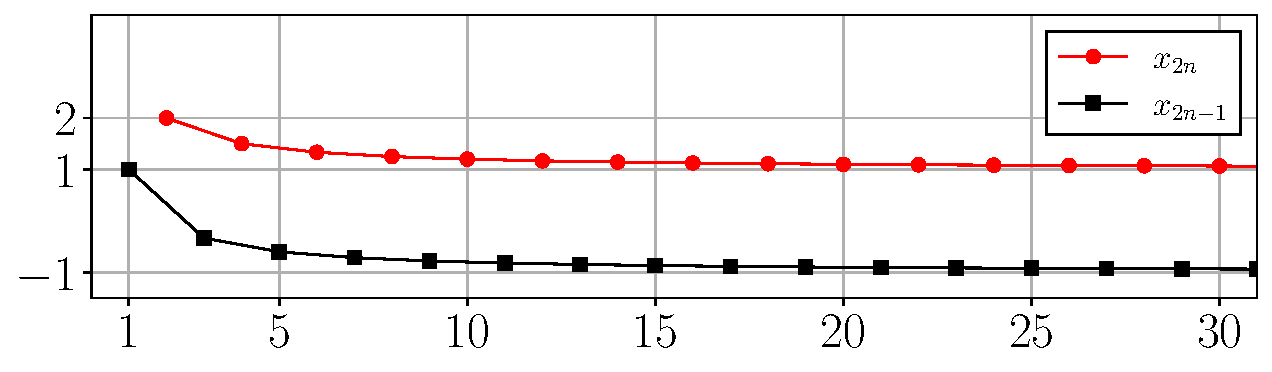
\includegraphics[width=0.85\textwidth]{UA_Figures/UA_ex3_2_2_fig_1.pdf}
            \caption{\( x_{2n} \) and \( x_{2n-1} \); \( A \) is the union of the red circles and the black squares}
            \label{fig:ex3.2.2_1}
        \end{figure}
        \noindent Now suppose that \( x \in \R \) is such that \( x \not\in \{ -1, 1 \} \); we claim that \( x \) is not a limit point of \( A \). First note that the distance from \( x \) to each of \( -1 \) and 1 is strictly positive, so that
        \[
            \epsilon := \min \{ \abs{x + 1}, \abs{x - 1} \} > 0.
        \]
        Since \( \lim x_{2n-1} = -1 \) and \( \lim x_{2n} = 1 \), the terms of \( (x_n) \) (i.e., the elements of \( A \)) must eventually be contained inside
        \[
            V_{\epsilon/2}(-1) \cup V_{\epsilon/2}(1) = \paren{ -1 - \frac{\epsilon}{2}, -1 + \frac{\epsilon}{2} } \cup \paren{ 1 - \frac{\epsilon}{2}, 1 + \frac{\epsilon}{2} }.
        \]
        Our choice of \( \epsilon \) is such that
        \[
            \bkt{ V_{\epsilon/2}(-1) \cup V_{\epsilon/2}(1) } \cap V_{\epsilon/2}(x) = \emptyset.
        \]
        \begin{figure}[H]
            \centering
            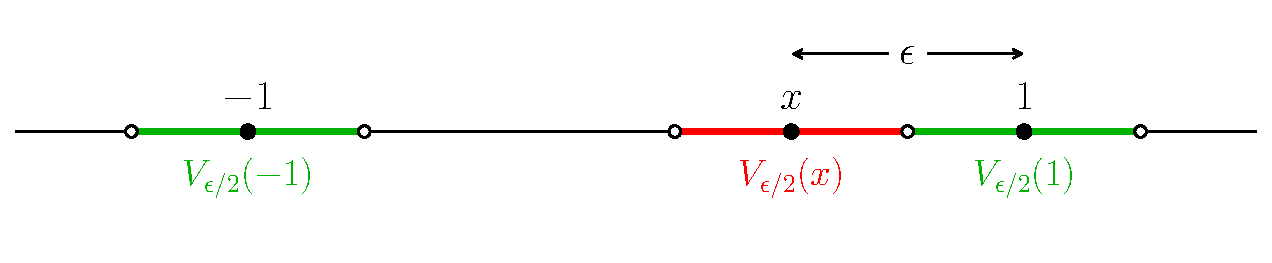
\includegraphics[width=0.85\textwidth]{UA_Figures/UA_ex3_2_2_fig_2.pdf}
            \caption{Special case where \( x \) is closer to 1 than to \( -1 \)}
            \label{fig:ex3.2.2_2}
        \end{figure}
        \noindent Thus there can be only finitely many elements of \( A \) in \( V_{\epsilon/2}(x) \); it follows that \( x \) cannot possibly be the limit of any sequence of elements of \( A \) distinct from \( x \), which by Theorem 3.2.5 is to say that \( x \) cannot be a limit point of \( A \). We may conclude that \( L_A = \{ -1, 1 \} \).

        \item \( A \) is not open. To see this, consider the point \( 2 \in A \). We claim that for any \( \epsilon > 0 \), the neighbourhood \( V_{\epsilon}(2) \) contains some \( x \not\in A \), so that \( V_{\epsilon}(2) \not\subseteq A \). It is straightforward to verify that every element \( a \in A \) satisfies \( a \leq 2 \) (see \Cref{fig:ex3.2.2_1}). Given this, if we let \( x = 2 + \tfrac{\epsilon}{2} \) then \( x \in V_{\epsilon}(2) \) and \( x \not\in A \).

        \( A \) is not closed either since it does not contain the limit point \( -1 \): for any \( n \in \N \) we have \( (-1)^n + \tfrac{2}{n} > -1 \) (see \Cref{fig:ex3.2.2_1}).

        \item Since \( L_A = \{ -1, 1 \}, 1 \in A \) and \( -1 \not\in A \), every point of \( A \) other than \( 1 \) is an isolated point of \( A \).

        \item The closure is
        \[
            \overline{A} = A \cup L_A = \{ -1 \} \cup \set{ (-1)^n + \frac{2}{n} : n = 1, 2, 3, \ldots }.
        \]
    \end{enumerate}

    Now let us consider the set \( B \).
    \begin{enumerate}
        \item Let \( L_B \) be the set of limit points of \( B \). We claim that \( L_B = [0, 1] \). To see this, first suppose that \( x \in [0, 1] \) and let \( \epsilon > 0 \) be given. Observe that
        \[
            V_{\epsilon}(x) \cap (0, 1) = (\max \{ x - \epsilon, 0 \}, \min \{ x + \epsilon, 1 \}).
        \]
        This is a proper interval contained in \( (0, 1) \) and hence, by the density of \( \Q \) in \( \R \), contains infinitely many elements of \( B \). It follows that \( x \) is a limit point of \( B \) and hence that \( [0, 1] \subseteq L_B \).
        
        If \( x \) is a limit point of \( B \) then by Theorem 3.2.5 it must be the case that \( x \) is the limit of a sequence of elements of \( B \). The Order Limit Theorem (Theorem 2.3.4) then implies that \( 0 \leq x \leq 1 \), so that \( L_B \subseteq [0, 1] \). We may conclude that \( L_B = [0, 1] \).

        \item \( B \) is not open, since for any \( x \in B \) and \( \epsilon > 0 \), the set \( V_{\epsilon}(x) \) will contain irrational numbers (Corollary 1.4.4) and hence cannot be contained in \( B \). \( B \) is also not closed, since it does not contain the limit point \( 0 \).

        \item \( B \) does not contain any isolated points, since \( B \subseteq L_B = [0, 1] \).

        \item We have \( \overline{B} = B \cup L_B = L_B = [0, 1] \).
    \end{enumerate}
\end{solution}

\begin{exercise}
\label{ex:3.2.3}
    Decide whether the following sets are open, closed, or neither. If a set is not open, find a point in the set for which there is no \( \epsilon \)-neighborhood contained in the set. If a set is not closed, find a limit point that is not contained in the set.
    \begin{enumerate}
        \item \( \Q \).

        \item \( \N \).

        \item \( \{ x \in \R : x \neq 0 \} \).

        \item \( \{ 1 + 1/4 + 1/9 + \cdots + 1/n^2 : n \in \N \} \).

        \item \( \{ 1 + 1/2 + 1/3 + \cdots + 1/n : n \in \N \} \).
    \end{enumerate}
\end{exercise}

\begin{solution}
    \begin{enumerate}
        \item \( \Q \) is neither open nor closed. To see that \( \Q \) fails to be open, observe that by Corollary 1.4.4, for any \( \epsilon > 0 \) there are infinitely many irrational numbers in \( V_{\epsilon}(0) = (-\epsilon, \epsilon) \); it follows that \( V_{\epsilon}(0) \) cannot be contained in \( \Q \). To see that \( \Q \) fails to be closed, observe that \( \sqrt{2} \not\in \Q \) is a limit point of \( \Q \) (Theorems 3.2.5 and 3.2.10).

        \item \( \N \) is closed but not open. To see that \( \N \) is not open, observe that for any \( \epsilon > 0 \) there are infinitely many non-integers in \( V_{\epsilon}(1) = (1 - \epsilon, 1 + \epsilon) \); it follows that \( V_{\epsilon}(1) \) cannot be contained in \( \N \). To see that \( \N \) is closed, we will show that \( \setcomp{\N} \) is open and appeal to Theorem 3.2.13. Note that
        \[
            \setcomp{\N} = (-\infty, 1) \cup \bigcup_{n=1}^{\infty} (n, n + 1) = \bigcup_{n=1}^{\infty} \paren{ (-n, -n + 2) \cup (n, n + 1) }.
        \]
        Since open intervals are open (Example 3.2.2 (ii)), we see that \( \setcomp{\N} \) is a union of open sets and hence is itself open (Theorem 3.2.3 (i)). (It is also straightforward to argue directly from Definition 3.2.1 that intervals of the form \( (-\infty, a) \) or \( (a, \infty) \) for \( a \in \R \) are open. Indeed, if \( x \in (-\infty, a) \), then observe that \( V_{\epsilon}(x) \subseteq (-\infty, a) \), where \( \epsilon = a - x \); a similar argument holds for \( (a, \infty) \).)

        \item If we let \( E \) be the set in question, then \( E \) is open since it is the union of two open sets, \( E = (-\infty, 0) \cup (0, \infty) \), but \( E \) is not closed: notice that \( \tfrac{1}{n} \in E \) for each \( n \in \N \) and \( \tfrac{1}{n} \to 0 \), so that 0 is a limit point of \( E \) (Theorem 3.2.5), but \( 0 \not\in E \).

        \item Let \( E \) be the set in question; we claim that \( E \) is not open. To see this, let \( \epsilon > 0 \) be given and note that each element \( x \in E \) satisfies \( x \geq 1 \). It follows that \( V_{\epsilon}(1) \) cannot be contained in \( E \), since it contains infinitely many real numbers \( x < 1 \).
        
        Now we claim that \( E \) is not closed. From Example 2.4.4, we know that \( 1 + \tfrac{1}{4} + \tfrac{1}{9} + \cdots \) converges to some \( L \in \R \). Observe that for any \( n \in \N \)
        \[
            L - \sum_{j=1}^n \frac{1}{j^2} = \sum_{j=n+1}^{\infty} \frac{1}{j^2} > \frac{1}{(n+1)^2} > 0,
        \]
        so that \( L \neq \sum_{j=1}^n \tfrac{1}{j^2} \) for any \( n \in \N \). This implies that \( L \) is a limit point of \( E \) (Theorem 3.2.5), and also that \( L \not\in E \); it follows that \( E \) is not closed.

        \item Let \( E \) be the set in question. As in part (d), we have \( V_{\epsilon}(1) \not\subseteq E \) for any \( \epsilon > 0 \) and thus \( E \) is not open. Unlike part (d), we claim that \( E \) is closed. Let \( s_n = \sum_{j=1}^n \tfrac{1}{n} \), so that \( E = \{ s_n : n \in \N \} \), and notice that if \( E \) had a limit point then the sequence \( (s_n) \) would contain a convergent subsequence (Theorem 3.2.5). However, from Example 2.4.5 we know that \( (s_n) \) is strictly increasing and unbounded. Since such sequences have no convergent subsequences (\Cref{lem:ex2.6.2}), we see that \( E \) has no limit points and hence is closed.
    \end{enumerate}
\end{solution}

\begin{exercise}
\label{ex:3.2.4}
    Let \( A \) be nonempty and bounded above so that \( s = \sup A \) exists.
    \begin{enumerate}
        \item Show that \( s \in \overline{A} \).

        \item Can an open set contain its supremum?
    \end{enumerate}
\end{exercise}

\begin{solution}
    \begin{enumerate}
        \item If \( s \in A \) then certainly \( s \in \overline{A} \), so suppose that \( s \not\in A \). For each \( n \in \N \) we may use Lemma 1.3.8 to choose some \( a_n \in A \) satisfying \( s - \tfrac{1}{n} < a_n < s \) (the last inequality is strict as \( s \not\in A \)). The Squeeze Theorem (\Cref{ex:2.3.3}) then implies that \( \lim a_n = s \) and thus \( s \) is a limit point of \( A \) by Theorem 3.2.5, whence \( s \in \overline{A} \).

        \item An open set cannot contain its supremum. To see this, suppose that \( A \) is open and \( x \) belongs to \( A \). There then exists an \( \epsilon > 0 \) such that \( V_{\epsilon}(x) \subseteq A \), which implies that \( x + \tfrac{\epsilon}{2} \in A \); it follows that \( x \) is not the supremum of \( A \).
    \end{enumerate}
\end{solution}

\begin{exercise}
\label{ex:3.2.5}
    Prove Theorem 3.2.8.
\end{exercise}

\begin{solution}
    Theorem 3.2.8 states that a set \( F \subseteq \R \) is closed if and only if every Cauchy sequence contained in \( F \) has a limit that is also an element of \( F \). 
    
    First suppose that every Cauchy sequence contained in \( F \) has a limit that is also an element of \( F \) and let \( x \in \R \) be a limit point of \( F \). By Theorem 3.2.5 there is a sequence \( (x_n) \) contained in \( F \) such that \( \lim x_n = x \); since convergent sequences are also Cauchy sequences (Theorem 2.6.4), our hypothesis then guarantees that \( x \in F \). Thus \( F \) contains each of its limit points, i.e., \( F \) is closed.

    Now suppose that there exists a Cauchy sequence \( (x_n) \) contained in \( F \) satisfying \( x := \lim x_n \not\in F \). As \( (x_n) \) is entirely contained in \( F \) and \( x \not\in F \), it must be the case that \( x_n \neq x \) for each \( n \in \N \); it follows from Theorem 3.2.5 that \( x \) is a limit point of \( F \). Thus \( F \) fails to contain one of its limit points, i.e., \( F \) is not closed.
\end{solution}

\begin{exercise}
\label{ex:3.2.6}
    Decide whether the following statements are true or false. Provide counterexamples for those that are false, and supply proofs for those that are true.
    \begin{enumerate}
        \item An open set that contains every rational number must necessarily be all of \( \R \).

        \item The Nested Interval Property remains true if the ``closed interval'' is replaced by ``closed set''.

        \item Every nonempty open set contains a rational number.

        \item Every bounded infinite closed set contains a rational number.

        \item The Cantor set is closed.
    \end{enumerate}
\end{exercise}

\begin{solution}
    \begin{enumerate}
        \item This is false. Consider the set \( \R \setminus \set{ \sqrt{2} } = \paren{ -\infty, \sqrt{2} } \cup \paren{ \sqrt{2}, \infty } \). This contains every rational number since \( \sqrt{2} \) is irrational and is an open set since it is the union of two open sets (Theorem 3.2.3 (i)).
        
        \item This is false. For a counterexample, consider the closed sets \( [n, \infty) \) for \( n \in \N \). These sets are nested, however the Archimedean Property (Theorem 1.4.2) shows that
        \[
            \bigcap_{n=1}^{\infty} [n, \infty) = \emptyset.
        \]

        \item This is true. Suppose that \( A \) is open and non-empty, so that there exists some \( x \in A \) and some \( \epsilon > 0 \) such that \( V_{\epsilon}(x) \subseteq A \). By the density of \( \Q \) in \( \R \) (Theorem 1.4.3), there are infinitely many rational numbers contained in \( V_{\epsilon}(x) \) and hence in \( A \).

        \item This is false. Consider the set
        \[
            E = \set{ \sqrt{2} } \cup \set{ \sqrt{2} + \frac{\sqrt{2}}{n} : n \in \N }.
        \]
        This is a bounded infinite set which contains only irrational numbers (notice that
        \[
            \sqrt{2} + \frac{\sqrt{2}}{n} = \sqrt{2} \paren{ \frac{n+1}{n} } \in \Q \implies \sqrt{2} \in \Q,
        \]
        which contradicts Theorem 1.1.1). An argument similar to the one given in \Cref{ex:3.2.2} (a) shows that \( \sqrt{2} \) is the only limit point of \( E \) and thus \( E \) is closed.

        \item This is true. Because each \( C_n \) is the union of \( 2^n \) closed intervals, Theorem 3.2.14 (i) implies that each \( C_n \) is closed. It follows that \( C = \bigcap_{n=1}^{\infty} C_n \) is an intersection of closed sets and hence is itself closed (Theorem 3.2.14 (ii)).
    \end{enumerate}
\end{solution}

\begin{exercise}
\label{ex:3.2.7}
    Given \( A \subseteq \R \), let \( L \) be the set of all limit points of \( A \).
    \begin{enumerate}
        \item Show that the set \( L \) is closed.

        \item Argue that if \( x \) is a limit point of \( A \cup L \), then \( x \) is a limit point of \( A \). Use this observation to furnish a proof for Theorem 3.2.12.
    \end{enumerate}
\end{exercise}

\begin{solution}
    \begin{enumerate}
        \item Suppose that \( x \in \R \) is a limit point of \( L \); we will show that \( x \) is a limit point of \( A \) also. Let \( \epsilon > 0 \) be given. Because \( x \) is a limit point of \( L \), there exists some \( y \in L \) such that \( 0 < \abs{x - y} < \tfrac{\epsilon}{2} \), and then since \( y \) is a limit point of \( A \), there exists some \( a \in A \) such that \( \abs{y - a} < \abs{x - y} \). Notice that:
        \begin{itemize}
            \item \( \abs{x - a} \leq \abs{x - y} + \abs{y - a} < 2 \abs{x - y} < \epsilon \), so that \( a \in V_{\epsilon}(x) \);

            \item \( \abs{x - a} \geq \abs{x - y} - \abs{y - a} > 0 \), so that \( a \neq x \).
        \end{itemize}
        Thus \( x \) is a limit point of \( A \), i.e., \( x \in L \). We may conclude that \( L \) is closed.

        \item Let \( \epsilon > 0 \) be given. Since \( x \) is a limit point of \( A \cup L \), the neighbourhood \( V_{\epsilon/2}(x) \) contains some \( y \in A \cup L \) such that \( y \neq x \). If \( y \in A \) then \( V_{\epsilon}(x) \) contains a point of \( A \) other than \( x \), and if \( y \in L \) then the argument given in part (a) shows that \( V_{\epsilon}(x) \) again contains a point of \( A \) other than \( x \); it follows that \( x \) is a limit point of \( A \).

        This shows that \( \overline{A} = A \cup L \) contains all of its limit points and hence is closed.
    \end{enumerate}
\end{solution}

\begin{exercise}
\label{ex:3.2.8}
    Assume \( A \) is an open set and \( B \) is a closed set. Determine if the following sets are definitely open, definitely closed, both, or neither.
    \begin{enumerate}
        \item \( \overline{A \cup B} \)

        \item \( A \setminus B = \{ x \in A : x \not\in B \} \)

        \item \( \setcomp{(\setcomp{A} \cup B)} \)

        \item \( (A \cap B) \cup (\setcomp{A} \cap B) \)

        \item \( \setcomp{\overline{A}} \cap \overline{\setcomp{A}} \)
    \end{enumerate}
\end{exercise}

\begin{solution}
    \begin{enumerate}
        \item \( \overline{A \cup B} \) is definitely closed, by Theorem 3.2.12. It may or may not be open. For example, if \( A = B = \R \), then \( \overline{A \cup B} = \R \) is open. If \( A = (0, 1) \) and \( B = [0, 1] \), then \( \overline{A \cup B} = [0, 1] \) is not open.

        \item Since \( A \setminus B = A \cap \setcomp{B} \) is the intersection of two open sets, \( A \setminus B \) is definitely open (Theorem 3.2.3 (ii)). It may or may not be closed. For example, if \( A = (0, 1) \) and \( B = [0, 1] \), then \( A \setminus B = \emptyset \) is closed. If \( A = (0, 1) \) and \( B = [2, 3] \), then \( A \setminus B = (0, 1) \) is not closed.

        \item \( \setcomp{A} \cup B \) is the union of two closed sets and hence is closed (Theorem 3.2.14 (i)). The complement \( \setcomp{(\setcomp{A} \cup B)} \) is then definitely open (Theorem 3.2.13). It may or may not be closed. For example, if \( A = B = \R \), then \( \setcomp{(\setcomp{A} \cup B)} = \setcomp{(\emptyset \cup \R)} = \setcomp{\R} = \emptyset \) is closed. If \( A = (0, 1) \) and \( B = \setcomp{A} = (-\infty, 0] \cup [1, \infty) \), then
        \[
            \setcomp{(\setcomp{A} \cup B)} = \setcomp{(\setcomp{A} \cup \setcomp{A})} = \setcomp{(\setcomp{A})} = A
        \]
        is not closed.

        \item This is simply the set \( B \), which is given as definitely closed. It may or may not be open; \( B = \R \) is closed and open, whereas \( B = [0, 1] \) is closed but not open.

        \item We claim that \( \setcomp{\overline{A}} \) is a subset of \( \overline{\setcomp{A}} \). To see this, let \( L_A \) be the set of limit points of \( A \) and let \( L_{\setcomp{A}} \) be the set of limit points of \( \setcomp{A} \). Notice that
        \[
            \setcomp{\overline{A}} = \setcomp{(A \cup L_A)} = \setcomp{A} \cap \setcomp{L_A} \hspaceand \overline{\setcomp{A}} = \setcomp{A} \cup L_{\setcomp{A}}.
        \]
        Our claim now follows since \( \setcomp{\overline{A}} \subseteq \setcomp{A} \subseteq \overline{\setcomp{A}} \). Given this, we have \( \setcomp{\overline{A}} \cap \overline{\setcomp{A}} = \setcomp{\overline{A}} \), which is the complement of a closed set and hence is definitely open (Theorem 3.2.13). It may or may not be closed. For example, if \( A = \emptyset \) then \( \setcomp{\overline{A}} = \setcomp{\emptyset} = \R \) is closed. If \( A = (-\infty, 0) \), then \( \setcomp{\overline{A}} = \setcomp{(-\infty, 0]} = (0, \infty) \) is not closed.
    \end{enumerate}
\end{solution}

\begin{exercise}[De Morgan's Laws]
\label{ex:3.2.9}
    A proof for De Morgan's Laws in the case of two sets is outlined in \Cref{ex:1.2.5}. The general argument is similar.
    \begin{enumerate}
        \item Given a collection of sets \( \{ E_{\lambda} : \lambda \in \Lambda \} \), show that
        \[
            \setcomp{\paren{ \bigcup_{\lambda \in \Lambda} E_{\lambda} }} = \bigcap_{\lambda \in \Lambda} \setcomp{E_{\lambda}} \hspaceand \setcomp{\paren{ \bigcap_{\lambda \in \Lambda} E_{\lambda} }} = \bigcup_{\lambda \in \Lambda} \setcomp{E_{\lambda}}.
        \]

        \item Now, provide the details for the proof of Theorem 3.2.14.
    \end{enumerate}
\end{exercise}

\begin{solution}
    \begin{enumerate}
        \item We have
        \begin{align*}
            x \in \setcomp{\paren{ \bigcup_{\lambda \in \Lambda} E_{\lambda} }} &\iff x \not\in \bigcup_{\lambda \in \Lambda} E_{\lambda} \\[2mm]
            &\iff x \not\in E_{\lambda} \text{ for all } \lambda \in \Lambda \\[2mm]
            &\iff x \in \setcomp{E_{\lambda}} \text{ for all } \lambda \in \Lambda \\[2mm]
            &\iff x \in \bigcap_{\lambda \in \Lambda} \setcomp{E_{\lambda}}.
        \end{align*}
        The equality \( \setcomp{\paren{ \bigcup_{\lambda \in \Lambda} E_{\lambda} }} = \bigcap_{\lambda \in \Lambda} \setcomp{E_{\lambda}} \) follows. Similarly,
        \begin{align*}
            x \in \setcomp{\paren{ \bigcap_{\lambda \in \Lambda} E_{\lambda} }} &\iff x \not\in \bigcap_{\lambda \in \Lambda} E_{\lambda} \\[2mm]
            &\iff x \not\in E_{\lambda'} \text{ for some } \lambda' \in \Lambda \\[2mm]
            &\iff x \in \setcomp{E_{\lambda'}} \text{ for some } \lambda' \in \Lambda \\[2mm]
            &\iff x \in \bigcup_{\lambda \in \Lambda} \setcomp{E_{\lambda}}.
        \end{align*}
        Thus \( \setcomp{\paren{ \bigcap_{\lambda \in \Lambda} E_{\lambda} }} = \bigcup_{\lambda \in \Lambda} \setcomp{E_{\lambda}} \).

        \item Suppose we have finitely many closed sets \( E_1, \ldots, E_n \) and let \( E = E_1 \cup \cdots \cup E_n \). It follows from part (a) that
        \[
            \setcomp{E} = \setcomp{(E_1 \cup \cdots \cup E_n)} = \setcomp{E_1} \cap \cdots \cap \setcomp{E_n}.
        \]
        Each \( \setcomp{E_i} \) is open, so Theorem 3.2.3 (ii) implies that \( \setcomp{E} \), which is a finite intersection of open sets, is also open; it then follows from Theorem 3.2.13 that \( E \) is closed.
        
        Now suppose that we have an arbitrary collection \( \{ E_{\lambda} : \lambda \in \Lambda \} \) of closed sets and let \( E = \bigcap_{\lambda \in \Lambda} E_{\lambda} \). By part (a), we have
        \[
            \setcomp{E} = \setcomp{\paren{ \bigcap_{\lambda \in \Lambda} E_{\lambda} }} = \bigcup_{\lambda \in \Lambda} \setcomp{E_{\lambda}}.
        \]
        Each \( \setcomp{E_{\lambda}} \) is open, so Theorem 3.2.3 (i) implies that \( \setcomp{E} \), which is an arbitrary union of open sets, is also open. Thus \( E \) is closed (Theorem 3.2.13).
    \end{enumerate}
\end{solution}

\begin{exercise}
\label{ex:3.2.10}
    Only one of the following three descriptions can be realized. Provide an example that illustrates the viable description, and explain why the other two cannot exist.
    \begin{enumerate}
        \item A countable set contained in \( [0, 1] \) with no limit points.

        \item A countable set contained in \( [0, 1] \) with no isolated points.

        \item A set with an uncountable number of isolated points.
    \end{enumerate}
\end{exercise}

\begin{solution}
    \begin{enumerate}
        \item This is impossible. Suppose that \( E \subseteq [0, 1] \) is countable, i.e., there is a bijection \( f : \N \to E \); for \( n \in \N \), let \( x_n = f(n) \). The sequence \( (x_n) \) is certainly bounded, so the Bolzano-Weierstrass Theorem (Theorem 2.5.5) implies that there is a convergent subsequence \( (x_{n_k}) \to x \) for some \( x \in [0, 1] \). It then follows from Theorem 3.2.5 that \( x \) is a limit point of \( E \). (If \( x_{n_k} = x \) for some \( k \in \N \), simply remove this term from the sequence; there can be at most one such \( k \) as \( f \) is injective, so this will not affect the convergence of the subsequence.)

        \item This is possible. Consider the countable set \( B = (0, 1) \cap \Q \) from \Cref{ex:3.2.2}: we showed there that \( B \) has no isolated points.

        \item This is impossible. Suppose that \( E \) is a subset of \( \R \) and let \( A \) be the set of isolated points of \( E \). If \( x \in A \), then there is an \( \epsilon > 0 \) such that \( V_{\epsilon}(x) \cap E = \{ x \} \). By the density of \( \Q \) in \( \R \), there exist rational numbers \( p, q \) such that \( x - \epsilon < p < x < q < x + \epsilon \). Thus, letting \( U_x = (p, q) \), we have \( U_x \cap E = \{ x \} \). Define \( f : A \to B \) by \( f(x) = U_x \), where
        \[
            B = \bigcup_{\substack{p, q \in \Q, \\ p < q}} \{ (p, q) \};
        \]
        Theorem 1.5.8 (ii) shows that \( B \) is a countable set. If we assume that \( A \) is uncountable, then the function \( f \) cannot possibly be injective. Therefore there must exist \( x \neq y \) in \( A \) such that \( f(x) = f(y) \), i.e., \( U_x = U_y \). This implies that
        \[
            \{ x \} = U_x \cap E = U_y \cap E = \{ y \} \implies x = y,
        \]
        contradicting \( x \neq y \). It follows that \( A \) cannot be uncountable.
    \end{enumerate}
\end{solution}

\begin{exercise}
\label{ex:3.2.11}
    \begin{enumerate}
        \item Prove that \( \overline{A \cup B} = \overline{A} \cup \overline{B} \).

        \item Does this result about closures extend to infinite unions of sets?
    \end{enumerate}
\end{exercise}

\begin{solution}
    \begin{enumerate}
        \item First, let us prove the following lemma.
        \begin{lemma}
        \label{lem:ex3.2.11}
            If \( A \) and \( B \) are subsets of \( \R \), then \( x \in \R \) is a limit point of \( A \cup B \) if and only if \( x \) is a limit point of \( A \) or \( x \) is a limit point of \( B \), i.e.,
            \[
                L_{A \cup B} = L_A \cup L_B,
            \]
            where \( L_{A \cup B}, L_A, \) and \( L_B \) are the collections of limit points of \( A \cup B, A, \) and \( B \).
        \end{lemma}
        \begin{proof}
            Suppose that \( x \in \R \) is a limit point of \( A \) and let \( \epsilon > 0 \) be given. Because \( x \in L_A \), there exists some \( a \in A \subseteq A \cup B \) such that \( a \in V_{\epsilon}(x) \) and \( a \neq x \). It follows that there is an element of \( A \cup B \) distinct from \( x \) and contained in \( V_{\epsilon}(x) \); as \( \epsilon \) was arbitrary, we see that \( x \) is also a limit point of \( A \cup B \). A similar argument shows that \( x \) is a limit point of \( A \cup B \) if \( x \) is a limit point of \( B \) and thus \( L_A \cup L_B \subseteq L_{A \cup B} \).

            Now suppose that \( x \) is not a limit point of \( A \) and not a limit point of \( B \), i.e., there exist positive real numbers \( \epsilon_1 \) and \( \epsilon_2 \) such that \( V_{\epsilon_1}(x) \cap A \subseteq \{ x \} \) and \( V_{\epsilon_2}(x) \cap B \subseteq \{ x \} \). If we let \( \epsilon = \min \{ \epsilon_1, \epsilon_2 \} \), then \( V_{\epsilon}(x) \cap (A \cup B) \subseteq \{ x \} \); it follows that \( x \) is not a limit point of \( A \cup B \). Thus
            \[
                x \not\in L_A \text{ and } x \not\in L_B \implies x \not\in L_{A \cup B}.
            \]
            The contrapositive of this implication gives us the inclusion \( L_{A \cup B} \subseteq L_A \cup L_B \).
        \end{proof}

        Now let us show that \( \overline{A \cup B} = \overline{A} \cup \overline{B} \). If \( x \in \overline{A \cup B} \), then either \( x \in A \cup B \) or \( x \) is a limit point of \( A \cup B \). If \( x \in A \cup B \) then certainly \( x \in \overline{A} \cup \overline{B} \), and if \( x \) is a limit point of \( A \cup B \) then by \Cref{lem:ex3.2.11} \( x \) is a limit point of \( A \) or a limit point of \( B \); in either case, \( x \in \overline{A} \cup \overline{B} \) and thus \( \overline{A \cup B} \subseteq \overline{A} \cup \overline{B} \).
        
        If \( x \in \overline{A} \cup \overline{B} \), then either \( x \in \overline{A} \) or \( x \in \overline{B} \). If \( x \in \overline{A} \), then either \( x \in A \) or \( x \) is a limit point of \( A \). If \( x \in A \), then certainly \( x \in \overline{A \cup B} \), and if \( x \) is a limit point of \( A \) then by \Cref{lem:ex3.2.11} \( x \) is a limit point of \( A \cup B \) and hence belongs to \( \overline{A \cup B} \). Similarly, if \( x \in \overline{B} \) then \( x \in \overline{A \cup B} \). Thus \( \overline{A} \cup \overline{B} \subseteq \overline{A \cup B} \) and we may conclude that \( \overline{A \cup B} = \overline{A} \cup \overline{B} \).

        \item The result does not extend to the infinite case. For a counterexample, consider the closed sets \( A_n := \bkt{ \tfrac{1}{n}, 1 } \) for \( n \in \N \):
        \[
            \overline{\bigcup_{n=1}^{\infty} A_n} = \overline{(0, 1]} = [0, 1] \quad \text{ but } \quad \bigcup_{n=1}^{\infty} \overline{A_n} = \bigcup_{n=1}^{\infty} A_n = (0, 1].
        \]
    \end{enumerate}
\end{solution}

\begin{exercise}
\label{ex:3.2.12}
    Let \( A \) be an uncountable set and let \( B \) be the set of real numbers that divides \( A \) into two uncountable sets; that is, \( s \in B \) if both \( \{ x : x \in A \text{ and } x < s \} \) and \( \{ x : x \in A \text{ and } x > s \} \) are uncountable. Show \( B \) is nonempty and open.
\end{exercise}

\begin{solution}
    Define the sets
    \begin{multline*}
        B_1 = \{ x \in \R : (-\infty, x) \cap A \text{ is uncountable} \} \\
        \text{and} \quad B_2 = \{ x \in \R : (x, \infty) \cap A \text{ is uncountable} \}.
    \end{multline*}
    We claim that \( B_1 \) is non-empty. To see this, suppose that \( B_1 = \emptyset \), i.e., for all \( x \in \R \) the intersection \( (-\infty, x) \cap A \) is either countable or finite, and observe that
    \[
        A = \R \cap A = \paren{ \bigcup_{n=1}^{\infty} (-\infty, n) } \cap A = \bigcup_{n=1}^{\infty} \big( (-\infty, n) \cap A \big).
    \]
    So we have expressed \( A \) as a countable union of countable or finite sets; it follows from Theorem 1.5.8 that \( A \) is countable or finite. Given that \( A \) is uncountable, it must be the case that \( B_1 \) is non-empty.

    Next we claim that \( B_1 \) is open. Let \( x \in B_1 \) be given, so that \( (-\infty, x) \cap A \) is uncountable. Note that for any \( y \in \R \) with \( y > x \) we must have \( y \in B_1 \) also, since
    \[
        \big( (-\infty, x) \cap A \big) \subseteq \big( (-\infty, y) \cap A \big).
    \]
    Given this, we would like to find an \( \epsilon > 0 \) such that \( x - \epsilon \in B_1 \); it will follow that \( (x - \epsilon, \infty) \subseteq B_1 \), so that \( V_{\epsilon}(x) \subseteq B_1 \). Seeking a contradiction, suppose that for every \( \epsilon > 0 \) it holds that \( x - \epsilon \not\in B_1 \). In particular we have \( x - \tfrac{1}{n} \not\in B_1 \) for each \( n \in \N \), so that \( \paren{ -\infty, x - \tfrac{1}{n} } \cap A \) is either countable or finite for each \( n \in \N \). Notice that
    \[
        (-\infty, x) \cap A = \bigcup_{n=1}^{\infty} \Big( \paren{ -\infty, x - \tfrac{1}{n} } \cap A \Big);
    \]
    it then follows from Theorem 1.5.8 that \( (-\infty, x) \cap A \) is countable or finite, which is a contradiction since \( x \in B_1 \). Thus there must exist an \( \epsilon > 0 \) such that \( x - \epsilon \in B_1 \). As noted above we then have \( V_{\epsilon}(x) \subseteq B_1 \) and so we may conclude that \( B_1 \) is open. Similar arguments show that \( B_2 \) is also non-empty and open.

    Now let us show that \( B_1 \cup B_2 = \R \). If \( x \in \R \) is such that \( x \not\in B_1 \) and \( x \not\in B_2 \), i.e., both \( (-\infty, x) \cap A \) and \( (x, \infty) \cap A \) are either countable or finite, then observe that
    \[
        A = \R \cap A = \big( (-\infty, x) \cap A \big) \cup \big( \{ x \} \cap A \big) \cup \big( (x, \infty) \cap A \big).
    \]
    Thus \( A \) is a union of three countable or finite sets and it follows from Theorem 1.5.8 that \( A \) is either countable or finite. Since \( A \) is given as uncountable, it must be the case that there is no such \( x \); that is, \( B_1 \cup B_2 = \R \).

    Finally, observe that \( B = B_1 \cap B_2 \). To see that \( B \) is non-empty, suppose otherwise, so that \( \setcomp{B_1} = B_2 \). This demonstrates that \( B_1 \) is closed as well as open (Theorem 3.2.13). However, since \( B_1 \) is non-empty and not equal to \( \R \) (since \( B_2 \) is non-empty), and these are the only sets which are both closed and open (see \Cref{ex:3.2.13}), this is a contradiction; it follows that \( B \) is non-empty. Furthermore, \( B \) is open since it is the union of two open sets (Theorem 3.2.3 (i)).
\end{solution}

\begin{exercise}
\label{ex:3.2.13}
    Prove that the only sets that are both open and closed are \( \R \) and the empty set \( \emptyset \).
\end{exercise}

\begin{solution}
    It will suffice to show that if \( E \subseteq \R \) is non-empty, open, and closed, then \( E = \R \). Since \( E \neq \emptyset \), there exists some \( x \in E \). Let
    \[
        S = \{ t \in \R : t \geq x \text{ and } [x, t] \subseteq E \}.
    \]
    Note that \( S \) is non-empty since \( x \in S \). We claim that \( S \) is unbounded above. To see this, suppose otherwise, so that \( s := \sup S \) exists. If \( s \in S \), then \( s \in E \). If \( s \not\in S \), then for any \( \epsilon > 0 \) there exists some \( t \in S \) such that \( s - \epsilon < t < s \) (Lemma 1.3.8; the second inequality is strict because \( s \not\in S \)). Since \( t \neq s \) and \( t \in S \) implies \( t \in E \), we see that for any \( \epsilon > 0, V_{\epsilon}(s) \cap E \) contains a point of \( E \) other than \( s \); that is, \( s \) is a limit point of \( E \). Since \( E \) is closed it follows that \( s \in E \).

    In either case, we have \( s \in E \). Since \( E \) is open, there exists an \( \epsilon > 0 \) such that \( (s - \epsilon, s + \epsilon) \subseteq E \). This implies that \( \bkt{ x, s + \tfrac{\epsilon}{2} } \subseteq E \), so that \( s + \tfrac{\epsilon}{2} \in S \), contradicting the fact that \( s \) is the supremum of \( S \). Hence \( S \) must be unbounded above and it follows that if \( t \geq x \), then \( t \in E \). A similar argument with the infimum of the set \( \{ t \in \R : t \leq x \text{ and } [t, x] \subseteq E \} \) shows that if \( t \leq x \), then \( t \in E \). Thus \( E = \R \).
\end{solution}

\begin{exercise}
\label{ex:3.2.14}
    A dual notion to the closure of a set is the interior of a set. The \textit{interior} of \( E \) is denoted \( \interior{E} \) and is defined as
    \[
        \interior{E} = \{ x \in E : \text{there exists } V_{\epsilon}(x) \subseteq E \}.
    \]
    Results about closures and interiors possess a useful symmetry.
    \begin{enumerate}
        \item Show that \( E \) is closed if and only if \( \overline{E} = E \). Show that \( E \) is open if and only if \( \interior{E} = E \).

        \item Show that \( \setcomp{\overline{E}} = \interior{(\setcomp{E})} \), and similarly that \( \setcomp{(\interior{E})} = \overline{\setcomp{E}} \).
    \end{enumerate}
\end{exercise}

\begin{solution}
    \begin{enumerate}
        \item Let \( L \) be the set of limit points of \( E \) and observe that \( E \cup L = E \) if and only if \( L \subseteq E \). This is exactly the statement that \( \overline{E} = E \) if and only if \( E \) is closed.

        Since \( \interior{E} \subseteq E \), it will suffice to show that \( E \) is open if and only if \( E \subseteq \interior{E} \). This is clear once we note that \( E \subseteq \interior{E} \) if and only if, for each \( x \in E \), there exists an \( \epsilon > 0 \) such that \( V_{\epsilon}(x) \subseteq E \).

        \item Let \( L \) be the set of limit points of \( E \) and observe that
        \begin{align*}
            x \in \setcomp{\overline{E}} &\iff x \in \setcomp{(E \cup L)} \\
            &\iff x \in \setcomp{E} \cap \setcomp{L} \\
            &\iff x \not\in E \text{ and } x \text{ is not a limit point of } E \\
            &\iff \text{there exists an } \epsilon > 0 \text{ such that } V_{\epsilon}(x) \cap E = \emptyset \\
            &\iff \text{there exists an } \epsilon > 0 \text{ such that } V_{\epsilon}(x) \subseteq \setcomp{E} \\
            &\iff x \in \interior{(\setcomp{E})}.
        \end{align*}
        Thus \( \setcomp{\overline{E}} = \interior{(\setcomp{E})} \). Similarly,
        \begin{align*}
            x \in \setcomp{(\interior{E})} &\iff x \not\in \interior{E} \\
            &\iff \text{for all } \epsilon > 0, V_{\epsilon}(x) \not\subseteq E \\
            &\iff \text{for all } \epsilon > 0, V_{\epsilon}(x) \cap \setcomp{E} \neq \emptyset \\
            &\iff (\text{for all } \epsilon > 0) (x \in \setcomp{E} \text{ or there exists } y \in V_{\epsilon}(x) \cap \setcomp{E} \text{ with } y \neq x) \\
            &\iff x \in \setcomp{E} \text{ or for all } \epsilon > 0 \text{ there exists } y \in V_{\epsilon}(x) \cap \setcomp{E} \text{ with } y \neq x \\
            &\iff x \in \setcomp{E} \text{ or } x \text{ is a limit point of } \setcomp{E} \\
            &\iff x \in \overline{\setcomp{E}}.
        \end{align*}
        Thus \( \setcomp{(\interior{E})} = \overline{\setcomp{E}} \).
    \end{enumerate}
\end{solution}

\begin{exercise}
\label{ex:3.2.15}
    A set \( A \) is called an \( F_{\sigma} \) set if it can be written as the countable union of closed sets. A set \( B \) is called a \( G_{\delta} \) set if it can be written as the countable intersection of open sets.
    \begin{enumerate}
        \item Show that a closed interval \( [a, b] \) is a \( G_{\delta} \) set.

        \item Show that the half-open interval \( (a, b] \) is both a \( G_{\delta} \) and an \( F_{\sigma} \) set.

        \item Show that \( \Q \) is an \( F_{\sigma} \) set, and the set of irrationals \( \I \) forms a \( G_{\delta} \) set. (We will see in Section 3.5 that \( \Q \) is \textit{not} a \( G_{\delta} \) set, nor is \( \I \) an \( F_{\sigma} \) set.)
    \end{enumerate}
\end{exercise}

\begin{solution}
    \begin{enumerate}
        \item Observe that
        \[
            [a, b] = \bigcap_{n=1}^{\infty} \paren{ a - \frac{1}{n}, b + \frac{1}{n} }.
        \]

        \item For any \( n \in \N \) the set \( \paren{ a - \tfrac{1}{n}, b + \tfrac{1}{n} } \setminus \{ a \} = \paren{ a - \tfrac{1}{n}, b + \tfrac{1}{n} } \cap \setcomp{\{ a \}} \) is the intersection of two open sets and hence is open. Observe that
        \[
            (a, b] = [a, b] \setminus \{ a \} = \paren{ \bigcap_{n=1}^{\infty} \paren{ a - \frac{1}{n}, b + \frac{1}{n} } } \setminus \{ a \} = \bigcap_{n=1}^{\infty} \paren{ \paren{ a - \frac{1}{n}, b + \frac{1}{n} } \setminus \{ a \} }.
        \]
        Thus \( (a, b] \) is a \( G_{\delta} \) set. Next, observe that for any \( n \in \N \) the set \( \bkt{ a + \tfrac{1}{n}, b - \tfrac{1}{n} } \cup \{ b \} \) is the union of two closed sets and hence is closed. Notice that
        \[
            (a, b] = \bigcup_{n=1}^{\infty} \paren{ \bkt{ a + \frac{1}{n}, b - \frac{1}{n} } \cup \{ b \} }.
        \]
        Thus \( (a, b] \) is an \( F_{\sigma} \) set.

        \item Observe that
        \[
            \Q = \bigcup_{r \in \Q} \{ r \}.
        \]
        Since \( \Q \) is countable, this demonstrates that \( \Q \) is an \( F_{\sigma} \) set. De Morgan's Laws (\Cref{ex:3.2.9}) imply that the complement of an \( F_{\sigma} \) set is a \( G_{\delta} \) set (and vice versa), so we have also shown that \( \I \) is a \( G_{\delta} \) set.
    \end{enumerate}
\end{solution}

\section{Compact Sets}
\label{sec:3.3}

\begin{exercise}
\label{ex:3.3.1}
    Show that if \( K \) is compact and nonempty, then \( \sup K \) and \( \inf K \) both exist and are elements of \( K \).
\end{exercise}

\begin{solution}
    \( K \) is given as non-empty and must be bounded by Theorem 3.3.8, so the Axiom of Completeness guarantees that \( \sup K \) and \( \inf K \) both exist. Suppose that \( \sup K \not\in K \). By Lemma 1.3.8, for each \( n \in \N \) there exists an \( x_n \in K \) satisfying
    \[
        \sup K - \frac{1}{n} < x_n < \sup K;
    \]
    the last inequality is strict as \( \sup K \not\in K \). The Squeeze Theorem (\Cref{ex:2.3.3}) and Theorem 3.2.5 now imply that \( \sup K \) is a limit point of \( K \); since \( \sup K \not\in K \), it follows that \( K \) is not closed, which contradicts Theorem 3.3.8. Thus \( \sup K \in K \), and a similar argument with the infimum and \Cref{ex:1.3.1} (b) shows that \( \inf K \in K \).
\end{solution}

\begin{exercise}
\label{ex:3.3.2}
    Decide which of the following sets are compact. For those that are not compact, show how Definition 3.3.1 breaks down. In other words, give an example of a sequence contained in the given set that does not possess a subsequence converging to a limit in the set.
    \begin{enumerate}
        \item \( \N \).

        \item \( \Q \cap [0, 1] \).

        \item The Cantor set.

        \item \( \{ 1 + 1/2^2 + 1/3^2 + \cdots + 1/n^2 : n \in \N \} \).

        \item \( \{ 1, 1/2, 2/3, 3/4, 4/5, \ldots \} \).
    \end{enumerate}
\end{exercise}

\begin{solution}
    \begin{enumerate}
        \item \( \N \) is not compact. Consider the sequence \( (1, 2, 3, \ldots) \), which is increasing and unbounded. As shown in \Cref{lem:ex2.6.2}, such sequences do not have convergent subsequences.

        \item \( \Q \cap [0, 1] \) is not compact. Let \( x = \tfrac{\sqrt{2}}{2} \in (0, 1) \). By Theorem 3.2.10, there is a sequence of rational numbers \( (x_n) \) converging to \( x \). Since \( 0 < x < 1 \), this sequence must eventually be contained in \( (0, 1) \). By removing a finite number of terms from the sequence if necessary, which will not affect convergence, we may assume that the sequence is entirely contained in \( \Q \cap [0, 1] \). It follows from Theorem 2.5.2 that every subsequence of \( (x_n) \) also converges to \( x \), which does not belong to \( \Q \cap [0, 1] \).

        \item The Cantor set \( C \) is compact by Theorem 3.3.8: \( C \) is closed by \Cref{ex:3.2.6} (e) and bounded as \( C \subseteq [0, 1] \).

        \item Let \( E \) be the set in question and let \( s_n = \sum_{j=1}^n \tfrac{1}{j^2} \). Certainly \( (s_n) \) is contained in \( E \) and from Example 2.4.4 we know that \( \lim s_n = L \) for some \( L \in \R \). As shown in \Cref{ex:3.2.3} (d), \( L \) does not belong to \( E \), and since all subsequences of \( s_n \) also converge to \( L \) (Theorem 2.5.2), we see that \( E \) is not compact.

        \item Let \( E \) be the set in question, i.e.,
        \[
            E = \{ 1 \} \cup \set{ 1 - \tfrac{1}{n} : n \in \N }.
        \]
        Using a similar argument to the one given in \Cref{ex:3.2.2}, we see that 1 is the only limit point of \( E \). It follows that \( E \) is closed and bounded, and hence compact (Theorem 3.3.8).
    \end{enumerate}
\end{solution}

\begin{exercise}
\label{ex:3.3.3}
    Prove the converse of Theorem 3.3.4 by showing that if a set \( K \subseteq \R \) is closed and bounded, then it is compact.
\end{exercise}

\begin{solution}
    Suppose that \( K \subseteq \R \) is closed and bounded. If \( (x_n) \) is an arbitrary sequence contained in \( K \), then \( (x_n) \) must be bounded and so the Bolzano-Weierstrass Theorem (Theorem 2.5.5) implies that there exists a subsequence \( (x_{n_k}) \) such that \( \lim_{k \to \infty} x_{n_k} = x \) for some \( x \in \R \); our aim is to show that \( x \in K \).
    
    If \( x \not\in K \) then \( x_{n_k} \neq x \) for each \( k \in \N \). It follows from Theorem 3.2.5 that \( x \) is a limit point of \( K \) which does not belong to \( K \), so that \( K \) is not closed. Thus
    \[
        x \not\in K \implies K \text{ not closed}.
    \]
    The contrapositive of this implication and the hypothesis that \( K \) is closed gives us \( x \in K \), as desired.
\end{solution}

\begin{exercise}
\label{ex:3.3.4}
    Assume \( K \) is compact and \( F \) is closed. Decide if the following sets are definitely compact, definitely closed, both, or neither.
    \begin{enumerate}
        \item \( K \cap F \)

        \item \( \overline{\setcomp{F} \cup \setcomp{K}} \)

        \item \( K \setminus F = \{ x \in K : x \not\in F \} \)

        \item \( \overline{K \cap \setcomp{F}} \)
    \end{enumerate}
\end{exercise}

\begin{solution}
    Throughout this exercise, we will repeatedly use that a subset of \( \R \) is compact if and only if it is closed and bounded (Theorem 3.3.8).
    \begin{enumerate}
        \item \( K \) is closed since it is compact, so \( K \cap F \) is the intersection of two closed sets and hence is definitely closed (Theorem 3.2.14 (ii)). Certainly the intersection of a bounded set with any other set is again bounded, so since \( K \) is bounded by virtue of being compact, we see that \( K \cap F \) is bounded as well as closed. It follows that \( K \cap F \) is definitely compact .

        \item The closure of any set is closed (Theorem 3.2.12), so \( \overline{\setcomp{F} \cup \setcomp{K}} \) is definitely closed. However, \( \overline{\setcomp{F} \cup \setcomp{K}} \) cannot be compact since it is unbounded. To see this, let us first show that if \( E \subseteq \R \) is bounded, then \( \setcomp{E} \) is unbounded. Since \( E \) is bounded, there exists an \( M > 0 \) such that \( E \subseteq [-M, M] \). It follows that \( ((-\infty, M) \cup (M, \infty)) \subseteq \setcomp{E} \), whence \( \setcomp{E} \) is unbounded. Returning to the set \( \overline{\setcomp{F} \cup \setcomp{K}} \), we have that \( K \) is bounded since it is compact and thus \( \setcomp{K} \) is unbounded. Since
        \[
            \setcomp{K} \subseteq \setcomp{F} \cup \setcomp{K} \subseteq \overline{\setcomp{F} \cup \setcomp{K}},
        \]
        we see that \( \overline{\setcomp{F} \cup \setcomp{K}} \) must also be unbounded. It follows that \( \overline{\setcomp{F} \cup \setcomp{K}} \) cannot be compact.

        \item Since \( K \) is bounded, \( K \setminus F \) must also be bounded, and hence \( K \setminus F \) is compact if and only if it is closed. \( K \setminus F \) could be compact/closed: for example, taking \( F = \emptyset \). \( K \setminus F \) could also fail to be compact/closed. For example, if we take \( K = [-2, 2] \) and \( F = [-1, 1] \), then \( K \setminus F = [-2, 1) \cup (1, 2] \), which is not compact/closed.

        \item First, notice that if \( E \subseteq \R \) is bounded by some \( M > 0 \), i.e., \( E \subseteq [-M, M] \), then since \( [-M, M] \) is closed it follows from Theorem 3.2.12 that \( \overline{E} \subseteq [-M, M] \) also, i.e., \( \overline{E} \) is also bounded by \( M \).

        Returning to the question, note that since \( K \) is bounded, \( K \cap \setcomp{F} \) must also be bounded. By the previous paragraph, it follows that \( \overline{K \cap \setcomp{F}} \) is bounded. Thus \( \overline{K \cap \setcomp{F}} \) is compact since it is closed and bounded.
    \end{enumerate}
\end{solution}

\begin{exercise}
\label{ex:3.3.5}
    Decide whether the following propositions are true or false. If the claim is valid, supply a short proof, and if the claim is false, provide a counterexample.
    \begin{enumerate}
        \item The arbitrary intersection of compact sets is compact.

        \item The arbitrary union of compact sets is compact.

        \item Let \( A \) be arbitrary, and let \( K \) be compact. Then, the intersection \( A \cap K \) is compact.

        \item If \( F_1 \supseteq F_2 \supseteq F_3 \supseteq F_4 \supseteq \cdots \) is a nested sequence of nonempty closed sets, then the intersection \( \bigcap_{n=1}^{\infty} F_n \neq \emptyset \).
    \end{enumerate}
\end{exercise}

\begin{solution}
    Throughout this exercise, we will repeatedly use that a subset of \( \R \) is compact if and only if it is closed and bounded (Theorem 3.3.8).
    \begin{enumerate}
        \item This is true. Suppose we have some collection \( \{ K_a : a \in A \} \) of compact sets. Each \( K_a \) must be closed and bounded and so the intersection \( K := \bigcap_{a \in A} K_a \) is also closed (Theorem 3.2.14 (ii)) and bounded. Thus \( K \) is compact.

        \item This is false. For each \( n \in \N \), let \( K_n = [0, n] \); each \( K_n \) is closed and bounded and hence compact. However, \( \bigcup_{n=1}^{\infty} K_n = [0, \infty) \), which is unbounded and hence not compact.

        \item This is false. If we let \( A = (0, 1) \) and \( K = [0, 1] \), then \( K \) is compact since it is closed and bounded but \( A \cap K = (0, 1) \), which is not closed and hence not compact.

        \item This is false; see \Cref{ex:3.2.6} (b) for a counterexample.
    \end{enumerate}
\end{solution}

\begin{exercise}
\label{ex:3.3.6}
    This exercise is meant to illustrate the point made in the opening paragraph to Section 3.3. Verify that the following three statements are true if every blank is filled in with the word ``finite.'' Which are true if every blank is filled in with the word ``compact''? Which are true if every blank is filled in with the word ``closed''?
    \begin{enumerate}
        \item Every \rule{1cm}{0.15mm} set has a maximum.

        \item If \( A \) and \( B \) are \rule{1cm}{0.15mm}, then \( A + B = \{ a + b : a \in A, b \in B \} \) is also \rule{1cm}{0.15mm}.

        \item If \( \{ A_n : n \in \N \} \) is a collection of \rule{1cm}{0.15mm} sets with the property that every finite subcollection has a nonempty intersection, then \( \bigcap_{n=1}^{\infty} A_n \) is nonempty as well.
    \end{enumerate}
\end{exercise}

\begin{solution}
    \begin{enumerate}
        \item Every non-empty finite set has a maximum by \Cref{lem:ex1.3.2}, and every non-empty compact set has a maximum by \Cref{ex:3.3.1}. However, not every closed set has a maximum: \( \R \) is closed but has no maximum element.

        \item If \( A \) is finite with \( m \) elements and \( B \) is finite with \( n \) elements, then \( A + B \) can have at most \( mn \) elements since the map \( A \times B \to A + B; \, (a, b) \mapsto a + b \) is a surjection. Thus \( A + B \) is also finite.

        If \( A \) and \( B \) are compact, then so is \( A + B \). To see this, let \( (x_n) \) be a sequence contained in \( A + B \), so that there are sequences \( (a_n) \) contained in \( A \) and \( (b_n) \) contained in \( B \) such that \( x_n = a_n + b_n \) for each \( n \in \N \). Since \( A \) is compact, the sequence \( (a_n) \) has a subsequence \( (a_{n_k}) \) such that \( \lim_{k \to \infty} a_{n_k} = a \) for some \( a \in A \). Since \( B \) is compact, the sequence \( (b_{n_k}) \) has a subsequence \( \paren{ b_{n_{k_{\ell}}} } \) such that \( \lim_{\ell \to \infty} b_{n_{k_{\ell}}} = b \) for some \( b \in B \). Observe that
        \[
            \lim_{\ell \to \infty} x_{n_{k_{\ell}}} = \lim_{\ell \to \infty} \paren{ a_{n_{k_{\ell}}} + b_{n_{k_{\ell}}} } = \lim_{\ell \to \infty} a_{n_{k_{\ell}}} + \lim_{\ell \to \infty} b_{n_{k_{\ell}}} = a + b \in A + B.
        \]
        It follows that \( A + B \) is compact.

        It is not necessarily the case that \( A + B \) is closed for closed sets \( A \) and \( B \). For a counterexample, let \( A = \N \) and let \( B = \set{ -n + \tfrac{1}{n} : n \in \N } \). For each \( n \in \N \), we have \( n + \paren{ -n + \tfrac{1}{n} } = \tfrac{1}{n} \in A + B \); it follows from Theorem 3.2.5 that 0 is a limit point of \( A + B \).
        
        Notice that, for \( n, k \in \Z \),
        \[
            n - k + \frac{1}{k} = 0 \iff k = 1 \text{ and } n = 0.
        \]
        Since any element of \( A + B \) is of the form \( n - k + \tfrac{1}{k} \) for some positive integers \( n, k \), we see that the limit point 0 fails to belong to \( A + B \). Thus \( A + B \) is not closed.

        \item Suppose \( \{ A_n : n \in \N \} \) is a collection of finite sets with the property that every finite subcollection has a non-empty intersection. For each \( k \in \N \), let \( m_k \) be the number of elements in \( \bigcap_{n=1}^k A_n \). By assumption, \( m_k \geq 1 \) for all \( k \in \N \). It is also clear that
        \[
            m_1 \geq m_2 \geq m_3 \geq \cdots \geq m_k \geq \cdots.
        \]
        By \Cref{lem:ex1.2.3}, this sequence must eventually be constant, i.e., there exists a positive integer \( K \) such that
        \[
            k \geq K \implies m_k = m_K \iff \bigcap_{n=1}^k A_n = \bigcap_{n=1}^K A_n.
        \]
        Since \( m_K \geq 1 \) there exists some \( x \in \bigcap_{n=1}^K A_n \), and since \( x \in \bigcap_{n=1}^k A_n \) for all \( k \geq K \) we then have \( x \in \bigcap_{n=1}^{\infty} A_n \).

        Suppose \( \{ A_n : n \in \N \} \) is a collection of compact sets with the property that every finite subcollection has a non-empty intersection. For \( m \in \N \) define \( K_m = \bigcap_{n=1}^m A_n \) and observe that each \( K_m \) is non-empty by assumption, each \( K_m \) is compact by \Cref{ex:3.3.5} (a), and the sequence \( (K_m) \) satisfies
        \[
            K_1 \supseteq K_2 \supseteq K_3 \supseteq \cdots \supseteq K_m \supseteq \cdots.
        \]
        It then follows from Theorem 3.3.5 that the intersection \( \bigcap_{m=1}^{\infty} K_m = \bigcap_{n=1}^{\infty} A_n \) is non-empty.

        For each \( n \in \N \), let \( A_n \) be the closed set \( [n, \infty) \). For a finite subcollection \( \{ A_{n_1}, \ldots, A_{n_m} \} \), we have
        \[
            \bigcap_{i=1}^m A_{n_i} = [N, \infty) \neq \emptyset,
        \]
        where \( N = \max_{1 \leq i \leq m} n_i \). However, \( \bigcap_{n=1}^{\infty} A_n = \emptyset \).
    \end{enumerate}
\end{solution}

\begin{exercise}
\label{ex:3.3.7}
    As some more evidence of the surprising nature of the Cantor set, follow these steps to show that the sum \( C + C = \{ x + y : x, y \in C \} \) is equal to the closed interval \( [0, 2] \). (Keep in mind that \( C \) has zero length and contains no intervals.)

    Because \( C \subseteq [0, 1], C + C \subseteq [0, 2], \) so we only need to prove the reverse inclusion \( [0, 2] \subseteq \{ x + y : x, y \in C \} \). Thus, given \( s \in [0, 2] \), we must find two elements \( x, y \in C \) satisfying \( x + y = s \).
    \begin{enumerate}
        \item Show that there exist \( x_1, y_1 \in C_1 \) for which \( x_1 + y_1 = s \). Show in general that, for an arbitrary \( n \in \N \), we can always find \( x_n, y_n \in C_n \) for which \( x_n + y_n = s \).

        \item Keeping in mind that the sequences \( (x_n) \) and \( (y_n) \) do not necessarily converge, show how they can nevertheless be used to produce the desired \( x \) and \( y \) in \( C \) satisfying \( x + y = s \).
    \end{enumerate}
\end{exercise}

\begin{solution}
    \begin{enumerate}
        \item If \( \tfrac{s}{2} \in C_1 = \bkt{ 0, \tfrac{1}{3} } \cup \bkt{ \tfrac{2}{3}, 1 } \) then take \( x_1 = y_1 = \tfrac{s}{2} \), and if \( \tfrac{s}{2} \in \paren{ \tfrac{1}{3}, \tfrac{2}{3} } \) then take \( x_1 = \tfrac{s}{2} - \tfrac{1}{3} \) and \( y_1 = \tfrac{s}{2} + \tfrac{1}{3} \). In either case, we have \( x_1, y_1 \in C_1 \) and \( x_1 + y_1 = s \). Geometrically, we have shown that for any \( s \in [0, 2] \), the line given by \( x + y = s \) must intersect the set \( C_1 \times C_1 \subseteq C_0 \times C_0 = [0, 1]^2 \); see \Cref{fig:ex3.3.7_1}, which shows the set \( C_1 \times C_1 \) as well as the lines \( x + y = s \) for several values of \( s \).

        \begin{figure}[H]
            \centering
            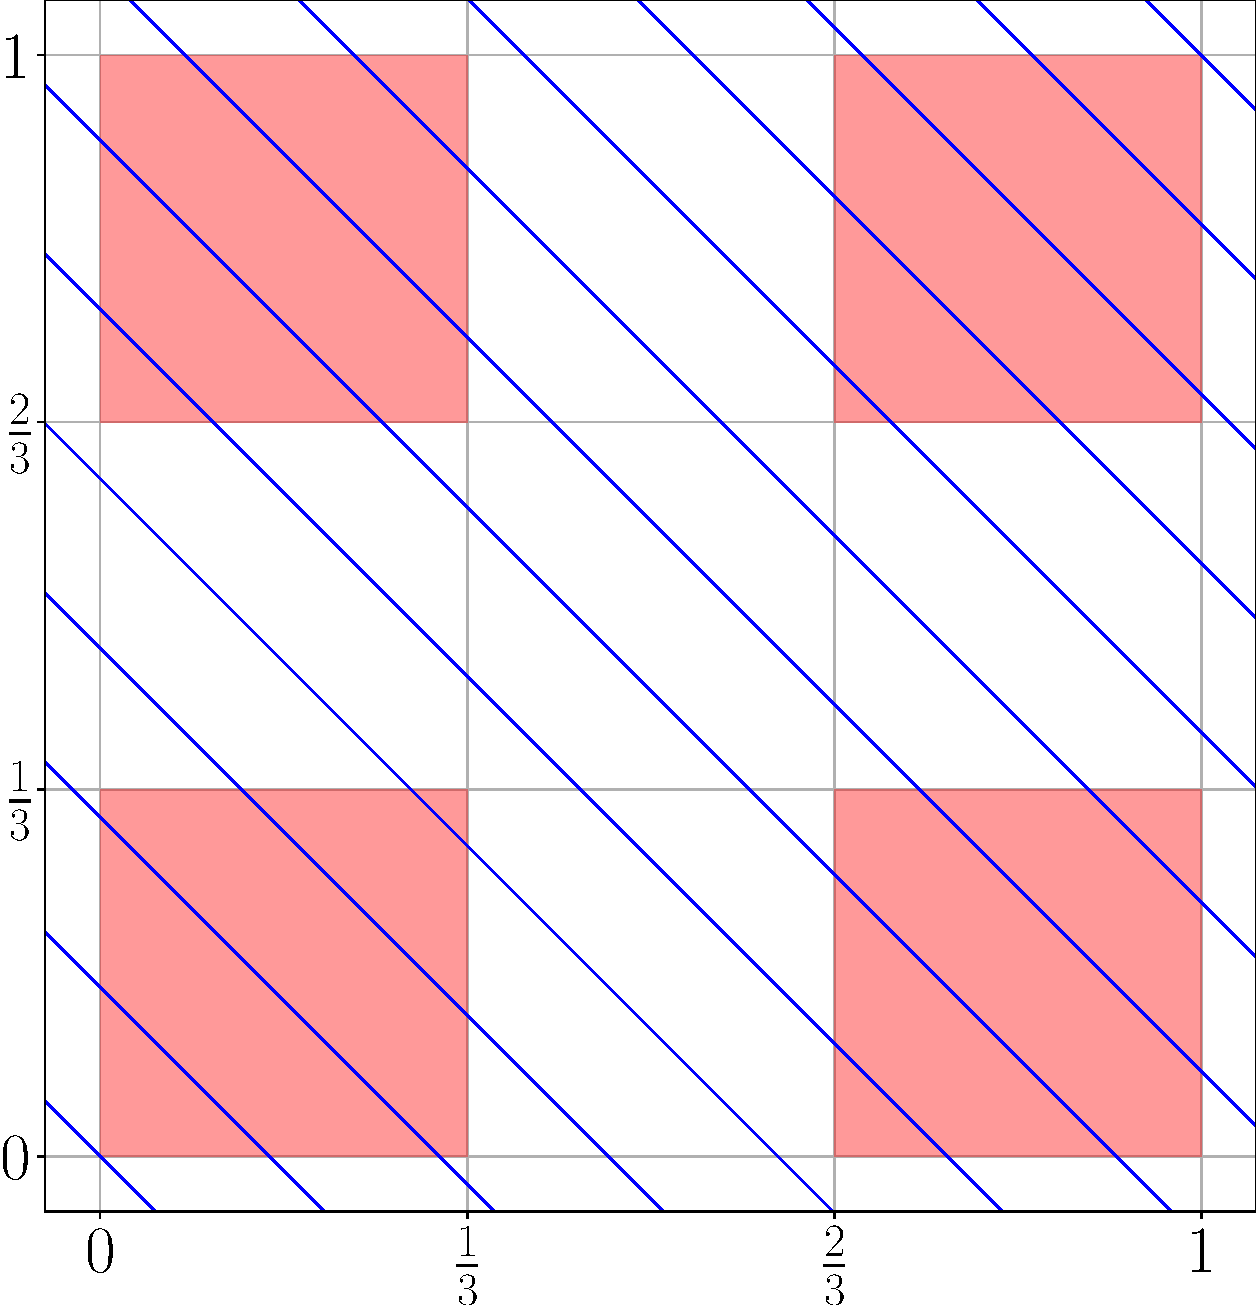
\includegraphics[width=0.6\textwidth]{UA_Figures/UA_ex3_3_7_fig_1.pdf}
            \caption{\( \textcolor{red}{C_1 \times C_1} \) and \( \textcolor{blue}{x + y = s} \) for various values of \( s \in [0, 2] \)}
            \label{fig:ex3.3.7_1}
        \end{figure}

        Let us argue inductively that for any \( n \in \N \) we can find \( x_n, y_n \in C_n \) such that \( x_n + y_n = s \). The base case \( n = 1 \) was handled above, so suppose that for some \( n \in \N \) we have \( x_n, y_n \in C_n \) such that \( x_n + y_n = s \). Since \( C_n \) consists of \( 2^n \) closed intervals each of length \( 3^{-n} \), the set \( C_n \times C_n \) consists of \( (2^n)^2 \) closed squares each with side length \( 3^{-n} \). Geometrically, the induction hypothesis guarantees that the line \( x + y = s \) intersects the set \( C_n \times C_n \) and thus must intersect one of the \( (2^n)^2 \) closed squares. Moving from \( C_n \) to \( C_{n+1} \), the middle third of each of the \( 2^n \) intervals is removed. This has the effect of splitting each of the \( (2^n)^2 \) squares of \( C_n \times C_n \) into four subsquares; see \Cref{fig:ex3.3.7_2}. \( C_{n+1} \times C_{n+1} \) then consists of the collection of these subsquares.
        
        Now we make the observation that this situation is essentially the same as in the base case: given that the line \( x + y = s \) intersects one of the squares of \( C_n \times C_n \), it must intersect at least one of the four subsquares after we remove the middle third of the sides of the square; see \Cref{fig:ex3.3.7_2} again. We are then guaranteed the existence of some \( x_{n+1}, y_{n+1} \in C_{n+1} \) such that \( x_{n+1} + y_{n+1} = s \). This completes the induction step.

        \begin{figure}[H]
            \centering
            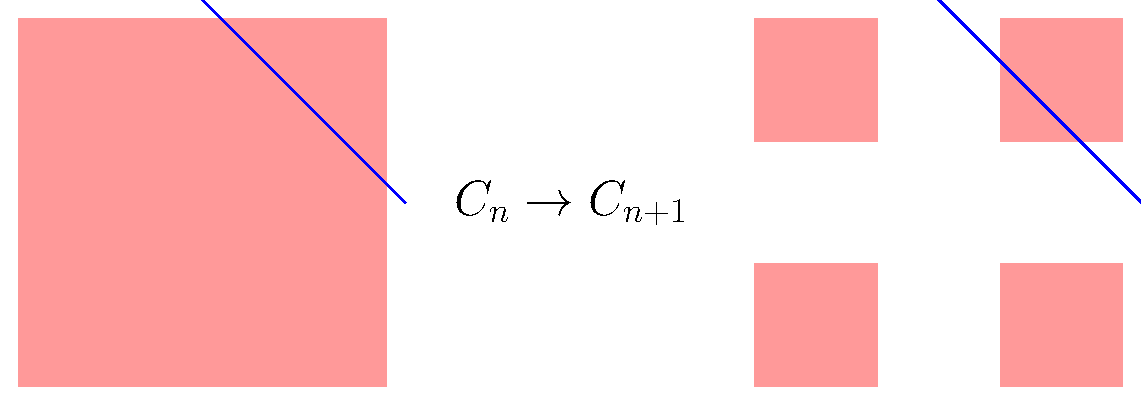
\includegraphics[width=0.8\textwidth]{UA_Figures/UA_ex3_3_7_fig_2.pdf}
            \caption{Subsquares of \( \textcolor{red}{C_n \times C_n} \) and \( \textcolor{red}{C_{n+1} \times C_{n+1}} \) intersecting the line \( \textcolor{blue}{x + y = s} \)}
            \label{fig:ex3.3.7_2}
        \end{figure}

        \item The sequence \( (x_n) \) is certainly bounded, so by the Bolzano-Weierstrass Theorem (Theorem 2.5.5) it has a convergent subsequence \( (x_{n_k}) \to x \) for some \( x \in \R \). Similarly, the sequence \( (y_{n_k}) \) is bounded and hence has a convergent subsequence \( \paren{ y_{n_{k_{\ell}}} } \to y \) for some \( y \in \R \). Since the sequence \( (C_n) \) is nested, we have \( x_{n_{k_{\ell}}} \in C_1 \) for all \( \ell \in \N \); it follows that \( x \in C_1 \) since \( C_1 \) is closed. The terms \( x_{n_{k_{\ell}}} \) belong to \( C_2 \) provided \( n_{k_{\ell}} \geq 2 \), i.e., all but a finite number of terms of \( \paren{ x_{n_{k_{\ell}}} } \) belong to \( C_2 \). Since \( C_2 \) is closed, it must then be the case that \( x \in C_2 \). Continuing in this fashion, we see that \( x \in C_n \) for all \( n \in \N \), i.e., \( x \in C \). Similarly, we obtain \( y \in C \). Now observe that on one hand,
        \[
            \lim_{\ell \to \infty} \paren{ x_{n_{k_{\ell}}} + y_{n_{k_{\ell}}} } = x + y.
        \]
        On the other hand,
        \[
            \lim_{\ell \to \infty} \paren{ x_{n_{k_{\ell}}} + y_{n_{k_{\ell}}} } = \lim_{\ell \to \infty} s = s.
        \]
        Since limits are unique (Theorem 2.2.7), we may conclude that \( x + y = s \).
    \end{enumerate}
\end{solution}

\begin{exercise}
\label{ex:3.3.8}
    Let \( K \) and \( L \) be nonempty compact sets, and define
    \[
        d = \inf \{ \abs{x - y} : x \in K \text{ and } y \in L \}.
    \]
    This turns out to be a reasonable definition for the \textit{distance} between \( K \) and \( L \).
    \begin{enumerate}
        \item If \( K \) and \( L \) are disjoint, show \( d > 0 \) and that \( d = \abs{x_0 - y_0} \) for some \( x_0 \in K \) and \( y_0 \in L \).

        \item Show that it's possible to have \( d = 0 \) if we assume only that the disjoint sets \( K \) and \( L \) are closed.
    \end{enumerate}
\end{exercise}

\begin{solution}
    \begin{enumerate}
        \item Let \( E = \{ \abs{x - y} : x \in K \text{ and } y \in L \} \) and notice that \( E \) is non-empty (since \( K \) and \( L \) are non-empty) and bounded below by 0; it follows that \( d = \inf E \) exists. By \Cref{ex:1.3.1} (b), for each \( n \in \N \) there exist elements \( x_n \in K \) and \( y_n \in L \) such that
        \[
            d \leq \abs{x_n - y_n} < d + \frac{1}{n}. \tag{1}
        \]
        Since \( (x_n) \) is entirely contained in the compact set \( K \), we are guaranteed the existence of a convergent subsequence \( (x_{n_k}) \to x_0 \) for some \( x_0 \in K \). Similarly, since the sequence \( (y_{n_k}) \) is entirely contained in the compact set \( L \), we are guaranteed the existence of a convergent subsequence \( \paren{ y_{n_{k_{\ell}}} } \to y_0 \) for some \( y_0 \in L \). We then have, by Theorem 2.5.2,
        \[
            \lim_{\ell \to \infty} \abs{x_{n_{k_{\ell}}} - y_{n_{k_{\ell}}}} = \abs{x_0 - y_0}.
        \]
        However, inequality (1) and the Squeeze Theorem (\Cref{ex:2.3.3}) imply that
        \[
            \lim_{\ell \to \infty} \abs{x_{n_{k_{\ell}}} - y_{n_{k_{\ell}}}} = d.    
        \]
        It follows from the uniqueness of limits (Theorem 2.2.7) that \( \abs{x_0 - y_0} = d \). Since \( K \) and \( L \) are disjoint, it must be the case that \( x_0 \neq y_0 \) and hence \( d > 0 \).

        \item Let \( K = \N \) and \( L = \set{ n + \tfrac{1}{n} : n \geq 2 } \) and observe that \( K \) and \( L \) are non-empty and disjoint. Furthermore, since
        \[
            \setcomp{K} = (-\infty, 1) \cup \bigcup_{n=1}^{\infty} (n, n + 1) \hspaceand \setcomp{L} = \paren{ -\infty, \frac{5}{2} } \cup \bigcup_{n=2}^{\infty} \paren{ n + \frac{1}{n}, n + 1 + \frac{1}{n + 1} },
        \]
        we see that \( \setcomp{K} \) and \( \setcomp{L} \) are both open (Theorem 3.2.3 (i)) and hence that \( K \) and \( L \) are both closed (Theorem 3.2.13). Letting \( E = \{ \abs{x - y} : x \in K \text{ and } y \in L \} \) again, note that for each \( n \geq 2 \), by taking \( n \in K \) and \( n + \tfrac{1}{n} \in L \), we have \( \tfrac{1}{n} \in E \). It follows that \( d = \inf E = 0 \).
    \end{enumerate}
\end{solution}

\begin{exercise}
\label{ex:3.3.9}
    Follow these steps to prove the final implication in Theorem 3.3.8.

    Assume \( K \) satisfies (i) and (ii), and let \( \{ O_{\lambda} : \lambda \in \Lambda \} \) be an open cover for \( K \). For contradiction, let's assume that no finite subcover exists. Let \( I_0 \) be a closed interval containing \( K \).
    \begin{enumerate}
        \item Show that there exists a nested sequence of closed intervals \( I_0 \supseteq I_1 \supseteq I_2 \supseteq \cdots \) with the property that, for each \( n \), \( I_n \cap K \) cannot be finitely covered and \( \lim \abs{I_n} = 0 \).

        \item Argue that there exists an \( x \in K \) such that \( x \in I_n \) for all \( n \).

        \item Because \( x \in K \), there must exist an open set \( O_{\lambda_0} \) from the original collection that contains \( x \) as an element. Explain how this leads to the desired contradiction.
    \end{enumerate}
\end{exercise}

\begin{solution}
    \begin{enumerate}
        \item Let us proceed by induction. For the base case, \( I_0 \cap K = K \) cannot be covered by any finite subcollection of \( \{ O_{\lambda} : \lambda \in \Lambda \} \) and we have \( \abs{I_0} = 2^0 \abs{I_0} \).
        
        Suppose that after \( n \) steps we have chosen nested closed intervals \( I_0 \supseteq I_1 \supseteq I_2 \supseteq \cdots \supseteq I_{n-1} \) such that, for each \( 0 \leq m \leq n - 1 \), \( I_m \cap K \) cannot be covered by any finite subcollection of \( \{ O_{\lambda} : \lambda \in \Lambda \} \) and \( \abs{I_m} = 2^{-m} \abs{I_0} \). Suppose that \( I_{n-1} = [a, c] \) and let \( b = \tfrac{a + c}{2} \). Note that if both of the sets \( [a, b] \cap K \) and \( [b, c] \cap K \) could be covered by a finite subcollection of \( \{ O_{\lambda} : \lambda \in \Lambda \} \), then \( I_{n-1} \cap K \) could also be finitely covered. By assumption this is not the case, so at least one of the intervals \( [a, b] \) or \( [b, c] \) must have the property that its intersection with \( K \) cannot be finitely covered. Let \( I_n \) be this interval and note that \( I_n \subseteq I_{n-1} \). Furthermore, since \( \abs{I_{n-1}} = 2^{-n + 1} \abs{I_0} \), we have \( \abs{I_n} = 2^{-n} \abs{I_0} \). This completes the induction step and we obtain the desired sequence of nested closed intervals.

        \item For each \( n \in \N, I_n \cap K \) is the intersection of two compact sets and hence is itself compact (\Cref{ex:3.3.5} (a)). Furthermore, since the sequence \( (I_n) \) is nested, the sequence \( (I_n \cap K) \) is also nested. It follows from Theorem 3.3.5 that there exists some \( x \in \bigcap_{n=1}^{\infty} (I_n \cap K) = K \cap \bigcap_{n=1}^{\infty} I_n \).

        \item Because \( x \) belongs to the open set \( O_{\lambda_0} \), there exists an \( \epsilon > 0 \) such that \( V_{\epsilon}(x) \subseteq O_{\lambda_0} \), and since \( \lim \abs{I_n} = 0 \) there exists an \( N \in \N \) such that \( \abs{I_N} < \tfrac{\epsilon}{2} \). Thus, since \( x \in I_N \), we must have \( I_N \subseteq V_{\epsilon}(x) \) and hence \( \paren{ I_N \cap K } \subseteq V_{\epsilon}(x) \). This implies that \( I_N \cap K \subseteq O_{\lambda_0} \), contradicting the fact that \( I_N \cap K \) cannot be covered by any finite subcollection of \( \{ O_{\lambda} : \lambda \in \Lambda \} \).
        \begin{center}
            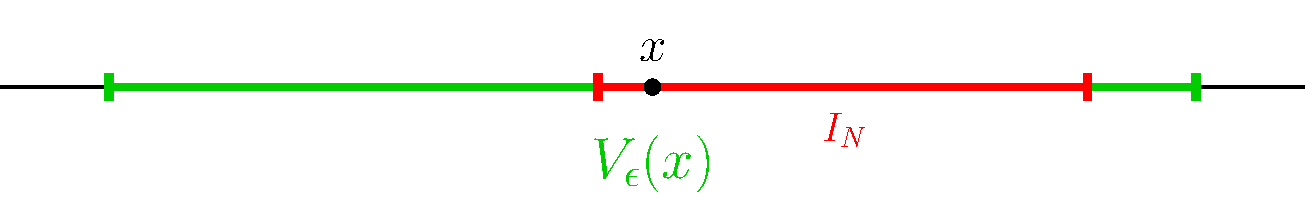
\includegraphics[width=0.69\textwidth]{UA_Figures/UA_ex3_3_9_fig.pdf}
        \end{center}
    \end{enumerate}
\end{solution}

\begin{exercise}
\label{ex:3.3.10}
    Here is an alternate proof to the one given in \Cref{ex:3.3.9} for the final implication in the Heine-Borel Theorem.

    Consider the special case where \( K \) is a closed interval. Let \( \{ O_{\lambda} : \lambda \in \Lambda \} \) be an open cover for \( [a, b] \) and define \( S \) to be the set of all \( x \in [a, b] \) such that \( [a, x] \) has a finite subcover from \( \{ O_{\lambda} : \lambda \in \Lambda \} \).
    \begin{enumerate}
        \item Argue that \( S \) is nonempty and bounded, and thus \( s = \sup S \) exists.

        \item Now show \( s = b \), which implies \( [a, b] \) has a finite subcover.

        \item Finally, prove the theorem for an arbitrary closed and bounded set \( K \).
    \end{enumerate}
\end{exercise}

\begin{solution}
    \begin{enumerate}
        \item Since \( a \in [a, b] \) there must be some \( O_{\lambda_0} \) such that \( a \in O_{\lambda_0} \), so that \( [a, a] \) is finitely covered; it follows that \( a \in S \). Evidently, \( S \) is bounded above by \( b \). Thus \( s = \sup S \) exists.

        \item Seeking a contradiction, suppose that \( s < b \), so that \( \epsilon_1 := \tfrac{b - s}{2} > 0 \). Since \( s \in [a, b] \), there exists some \( O_{\lambda_0} \) such that \( s \in O_{\lambda_0} \) and thus there is an \( \epsilon_2 > 0 \) such that \( V_{\epsilon_2}(s) \subseteq O_{\lambda_0} \). Let \( \epsilon := \min \{ \epsilon_1, \epsilon_2 \} > 0 \). By Lemma 1.3.8 there exists an \( x \in S \) such that \( s - \epsilon < x \leq s \), so that \( x \in V_{\epsilon}(s) \) and
        \[
            [a, x] \subseteq O_{\lambda_1} \cup \cdots \cup O_{\lambda_n}
        \]
        for some finite subcollection \( \{ O_{\lambda_1}, \ldots, O_{\lambda_n} \} \). Observe that \( s + \tfrac{\epsilon}{2} \leq s + \tfrac{\epsilon_1}{2} = \tfrac{s + b}{2} \in [a, b] \) and
        \[
            \bkt{ a, s + \tfrac{\epsilon}{2} } \subseteq V_{\epsilon}(s) \cup [a, x] \subseteq V_{\epsilon_2}(s) \cup [a, x] \subseteq O_{\lambda_0} \cup O_{\lambda_1} \cup \cdots \cup O_{\lambda_n}.
        \]
        It follows that \( s + \tfrac{\epsilon}{2} \in S \), contradicting the fact that \( s \) is the supremum of \( S \). Hence it must be the case that \( s = b \).

        This implies that \( [a, b] \) has a finite subcover: since \( b \in [a, b] \) there must be some \( O_{\lambda_0} \) such that \( b \in O_{\lambda_0} \) and hence some \( \epsilon > 0 \) such that \( V_{\epsilon}(b) \subseteq O_{\lambda_0} \), and since \( \sup S = b \) there is some \( x \in S \) such that \( b - \epsilon < x \leq b \) and
        \[
            [a, x] \subseteq O_{\lambda_1} \cup \cdots \cup O_{\lambda_n}
        \]
        for some finite subcollection \( \{ O_{\lambda_1}, \ldots, O_{\lambda_n} \} \). It follows that
        \[
            [a, b] \subseteq V_{\epsilon}(b) \cup [a, x] \subseteq O_{\lambda_0} \cup O_{\lambda_1} \cup \cdots \cup O_{\lambda_n}.
        \]

        \item Let \( \{ O_{\lambda} : \lambda \in \Lambda \} \) be an arbitrary open cover of \( K \). Since \( K \) is bounded, it is contained in some closed interval \( [a, b] \). Note that since \( K \) is closed, the collection \( \{ \setcomp{K} \} \cup \{ O_{\lambda} : \lambda \in \Lambda \} \) is an open cover of \( \R \) and hence of \( [a, b] \); by part (b), there then exists a finite subcover of \( [a, b] \). Since \( K \) is contained in \( [a, b] \), this finite subcover must also cover \( K \), and since \( \setcomp{K} \) evidently does not cover \( K \), this finite subcover must contain some sets \( O_{\lambda_1}, \ldots, O_{\lambda_n} \). It follows that \( K \) is covered by the finite collection \( O_{\lambda_1}, \ldots, O_{\lambda_n} \).
    \end{enumerate}
\end{solution}

\begin{exercise}
\label{ex:3.3.11}
    Consider each of the sets listed in \Cref{ex:3.3.2}. For each one that is not compact, find an open cover for which there is no finite subcover.
\end{exercise}

\begin{solution}
    The sets from \Cref{ex:3.3.2} which are not compact are \( \N, \Q \cap [0, 1], \) and
    \[
        E = \set{ 1 + \frac{1}{2^2} + \frac{1}{3^2} + \cdots + \frac{1}{k^2} : k \in \N }.
    \]
    Let us consider \( \N \) first. For each \( n \in \N \), let \( O_n = \paren{ n - 1, n + 1 } \), so that the collection \( \{ O_n : n \in \N \} \) covers \( \N \). Since each \( n \in \N \) belongs to exactly the set \( O_n \) and no others, there are in fact no proper subcovers, finite or otherwise.

    Next, let us consider \( \Q \cap [0, 1] \). Let \( y \) be the irrational number \( \tfrac{\sqrt{2}}{2} \in (0, 1) \). For each \( n \in \N \), define
    \[
        O_n = \paren{ -\infty, y - \frac{1}{n} } \cup \paren{ y + \frac{1}{n}, \infty }
    \]
    and notice that \( \bigcup_{n=1}^{\infty} O_n = \R \setminus \{ y \} \); it follows that the collection \( \{ O_n : n \in \N \} \) covers \( \Q \cap [0, 1] \) since \( y \) is irrational. We claim that there can be no finite subcover. If \( \{ O_{n_1}, \ldots, O_{n_m} \} \) is some finite subcollection, then let \( N = \max \{ n_1, \ldots, n_m \} \) and observe that
    \[
        \bigcup_{i=1}^m O_{n_i} = \paren{ -\infty, y - \frac{1}{N} } \cup \paren{ y + \frac{1}{N}, \infty }.
    \]
    Since
    \[
        \bkt{ y - \frac{1}{N}, y + \frac{1}{N} } \cap [0, 1] = \bkt{ \max \set{ 0, y - \tfrac{1}{N} }, \min \set{ 1, y + \tfrac{1}{N} } },
    \]
    which is a proper interval, we are guaranteed by the density of \( \Q \) in \( \R \) (Theorem 1.4.3) the existence of a rational number \( p \in \bkt{ y - \tfrac{1}{N}, y + \tfrac{1}{N} } \cap [0, 1] \). It follows that \( \Q \cap [0, 1] \not\subseteq \bigcup_{i=1}^m O_{n_i} \).

    Now let us consider the set \( E = \{ s_k : k \in \N \} \), where \( s_k = \sum_{j=1}^k \tfrac{1}{j^2} \). We know by the Monotone Convergence Theorem (Theorem 2.4.2) that \( L := \lim s_k \) is the supremum of \( E \). Furthermore, as noted in \Cref{ex:3.2.2}, \( L \) does not belong to \( E \). For each \( n \in \N \), let \( O_n = \paren{ -\infty, L - \tfrac{1}{n} } \) and note that
    \[
        \bigcup_{n=1}^{\infty} O_n = (-\infty, L),
    \]
    which must cover \( E \) since \( L \) is the supremum of \( E \) but does not belong to \( E \). We claim that there cannot exist a finite subcover. If \( \{ O_{n_1}, \ldots, O_{n_m} \} \) is some finite subcollection, then let \( N = \max \{ n_1, \ldots, n_m \} \) and observe that
    \[
        \bigcup_{i=1}^m O_{n_i} = \paren{ -\infty, L - \tfrac{1}{N} }.
    \]
    Since \( \lim s_k = L \), the sequence \( (s_k) \) must eventually be contained in the interval \( \paren{ L - \tfrac{1}{N}, L + \tfrac{1}{N} } \) and it follows that \( \{ O_{n_1}, \ldots, O_{n_m} \} \) cannot cover \( E \).
\end{solution}

\begin{exercise}
\label{ex:3.3.12}
    Using the concept of open covers (and explicitly avoiding the Bolzano-Weierstrass Theorem), prove that every bounded infinite set has a limit point.
\end{exercise}

\begin{solution}
    We will prove the contrapositive statement. That is, if \( E \subseteq \R \) is bounded, then
    \[
        E \text{ has no limit points} \implies E \text{ is finite}.
    \]
    If \( E \) is empty, we are done. Otherwise, each \( x \in E \) must be an isolated point, i.e., there exists some \( \epsilon_x > 0 \) such that \( V_{\epsilon_x}(x) \cap E = \{ x \} \). Notice that the collection \( \{ V_{\epsilon_x}(x) : x \in E \} \) is an open cover of \( E \). Since \( E \) has no limit points, \( E \) must be closed; the Heine-Borel Theorem (Theorem 3.3.8) then implies that there exist finitely many points \( \{ x_1, \ldots, x_n \} \) such that
    \[
        E \subseteq V_{\epsilon_{x_1}}(x_1) \cup \cdots \cup V_{\epsilon_{x_n}}(x_n).
    \]
    This implies that
    \begin{multline*}
        E = E \cap (V_{\epsilon_{x_1}}(x_1) \cup \cdots \cup V_{\epsilon_{x_n}}(x_n)) = (V_{\epsilon_{x_1}}(x_1) \cap E) \cup \cdots \cup (V_{\epsilon_{x_n}}(x_n) \cap E) \\[2mm]
        = \{ x_1 \} \cup \cdots \cup \{ x_n \} = \{ x_1, \ldots, x_n \}.
    \end{multline*}
    Thus \( E \) is finite.
\end{solution}

\begin{exercise}
\label{ex:3.3.13}
    Let's call a set \textit{clompact} if it has the property that every \textit{closed} cover (i.e., a cover consisting of closed sets) admits a finite subcover. Describe all of the clompact subsets of \( \R \).
\end{exercise}

\begin{solution}
    Let \( E \) be a subset of \( \R \). Suppose that \( E \) is finite. If \( E \) is empty then certainly \( E \) is clompact, so suppose that \( E = \{ x_1, \ldots, x_n \} \) and let \( \{ F_{\lambda} : \lambda \in \Lambda \} \) be a closed cover of \( E \). For each \( x_i \in E \), there is some \( F_{\lambda_i} \) such that \( x_i \in F_{\lambda_i} \); it follows that \( \{ F_{\lambda_1}, \ldots, F_{\lambda_n} \} \) is a finite subcover of \( E \) and hence that \( E \) is clompact.

    Now suppose that \( E \) is infinite and consider the closed cover \( \{ \{ x \} : x \in E \} \) of \( E \). Since \( E \) is infinite, finitely many singletons cannot possibly cover \( E \). So we have found a closed cover of \( E \) which cannot have a finite subcover and hence \( E \) is not clompact.

    To conclude, the clompact subsets of \( \R \) are precisely the finite subsets of \( \R \).
\end{solution}

\section{Perfect Sets and Connected Sets}
\label{sec:3.4}

\begin{exercise}
\label{ex:3.4.1}
    If \( P \) is a perfect set and \( K \) is compact, is the intersection \( P \cap K \) always compact? Always perfect?
\end{exercise}

\begin{solution}
    \( P \) is closed, so \( P \cap K \) must be compact (\Cref{ex:3.3.4} (a)). However, \( P \cap K \) need not be perfect. For a counterexample, consider \( P = [0, 1] \) and \( K = \{ 0 \} \).
\end{solution}

\begin{exercise}
\label{ex:3.4.2}
    Does there exist a perfect set consisting of only rational numbers?
\end{exercise}

\begin{solution}
    No. By Theorem 3.4.3, a non-empty perfect set must be uncountable, but any subset of \( \Q \) is either finite or countably infinite (Theorem 1.5.6 (i) and Theorem 1.5.7). (Strictly speaking, the empty set is both perfect and a subset of the rationals; I suspect this is not what Abbott had in mind.)
\end{solution}

\begin{exercise}
\label{ex:3.4.3}
    Review the portion of the proof given in Example 3.4.2 and follow these steps to complete the argument.
    \begin{enumerate}
        \item Because \( x \in C_1 \), argue that there exists an \( x_1 \in C \cap C_1 \) with \( x_1 \neq x \) satisfying \( \abs{x - x_1} \leq 1/3 \).

        \item Finish the proof by showing that for each \( n \in \N \), there exists \( x_n \in C \cap C_n \), different from \( x \) satisfying \( \abs{x - x_n} \leq 1/3^n \).
    \end{enumerate}
\end{exercise}

\begin{solution}
    \begin{enumerate}
        \item We have \( C_1 = \bkt{ 0, \tfrac{1}{3} } \cup \bkt{ \tfrac{2}{3}, 1 } \). The endpoints of these intervals are never removed at any subsequent stage of the construction of the Cantor set, so they belong to \( C \). Since \( x \in C_1 \), it must belong to one of these intervals, say the interval \( \bkt{ 0, \tfrac{1}{3} } \). If \( 0 \leq x < \tfrac{1}{3} \), then take \( x_1 = \tfrac{1}{3} \), and if \( x = \tfrac{1}{3} \), then take \( x_1 = 0 \). We can make similar choices if \( x \in \bkt{ \tfrac{2}{3}, 1 } \). In any case, we have chosen an \( x_1 \in C \cap C_1 \) with \( x_1 \neq x \) satisfying \( \abs{x - x_1} \leq \tfrac{1}{3} \).

        \item Let \( n \in \N \) be given. The set \( C_n \) consists of \( 2^n \) disjoint closed intervals each of length \( \tfrac{1}{3^n} \). The endpoints of these intervals are never removed at any subsequent stage of the construction of the Cantor set, so they belong to \( C \). Since \( x \in C \), we have \( x \in C_n \) and hence \( x \) must belong to one of the disjoint closed intervals, say \( I = [a, b] \) where \( b - a = \tfrac{1}{3^n} \). If \( a \leq x < b \), then let \( x_n = b \), and if \( x = b \) then let \( x_n = a \). In either case, we have chosen an \( x_n \in C \cap C_n \) such that \( x \neq x_n \) and \( \abs{x - x_n} \leq b - a = \tfrac{1}{3^n} \).

        Thus, by the Squeeze Theorem (\Cref{ex:2.3.3}), \( x \) is the limit of a sequence \( (x_n) \) contained in \( C \) such that \( x_n \neq x \) for all \( n \in \N \). It follows from Theorem 3.2.5 that \( x \) is a limit point of \( C \) and hence that \( C \) contains no isolated points.
    \end{enumerate}
\end{solution}

\begin{exercise}
\label{ex:3.4.4}
    Repeat the Cantor construction from Section 3.1 starting with the interval \( [0, 1] \). This time, however, remove the open middle \textit{fourth} from each component.
    \begin{enumerate}
        \item Is the resulting set compact? Perfect?

        \item Using the algorithms from Section 3.1, compute the length and dimension of this Cantor-like set.
    \end{enumerate}
\end{exercise}

\begin{solution}
    We begin with \( B_0 := [0, 1] \) and remove the open middle fourth to obtain \( B_1 = \bkt{ 0, \tfrac{3}{8} } \cup \bkt{ \tfrac{5}{8}, 1 } \). Notice that each interval has length \( \tfrac{3}{8} \). Next we remove the open middle fourth from each of the two intervals of \( B_1 \) to obtain
    \[
        B_2 = \paren{ \bkt{ 0, \frac{9}{64} } \cup \bkt{ \frac{15}{64}, \frac{24}{64} } } \cup \paren{ \bkt{ \frac{40}{64}, \frac{49}{64} } \cup \bkt{ \frac{55}{64}, 1 } }.
    \]
    Notice that each interval has length \( \paren{ \tfrac{3}{8} }^2 \). We continue in this fashion, obtaining sets \( B_n \) consisting of \( 2^n \) disjoint closed intervals each of length \( \paren{ \tfrac{3}{8} }^n \), and define our Cantor-like set \( B := \bigcap_{n=0}^{\infty} B_n \).
    \begin{enumerate}
        \item The set \( B \) is compact and perfect; the arguments used for the Cantor set work equally well for \( B \). Each \( B_n \) is closed, being a finite union of closed intervals, and thus \( B \) is an intersection of closed sets and hence is itself closed. Certainly \( B \) is bounded and so it follows from the Heine-Borel Theorem (Theorem 3.3.8) that \( B \) is compact.
        
        As in \Cref{ex:3.4.3}, given any \( x \in B \) we can find a sequence of endpoints \( (x_n) \) such that \( x_n \in B, x_n \neq x, \) and \( \abs{x - x_n} \leq \paren{ \tfrac{3}{8} }^n \) for each \( n \in \N \). It follows from the Squeeze Theorem (\Cref{ex:2.3.3}) and Theorem 3.2.5 that \( x \) is a limit point of \( B \) and hence that \( B \) has no isolated points. Since \( B \) is also closed, we see that \( B \) is a perfect set.

        \item At the first stage, we remove an interval of length \( \tfrac{1}{4} \). At the \( n \)\ts{th} stage (\( n = 2, 3, 4 \ldots \)), we remove \( 2^{n-1} \) intervals each of length \( \tfrac{1}{4} \paren{ \tfrac{3}{8} }^{n-1} \). Thus the length of \( B \) is
        \begin{multline*}
            1 - \paren{ \frac{1}{4} + 2 \cdot \frac{1}{4} \cdot \frac{3}{8} + 2^2 \cdot \frac{1}{4} \cdot \paren{ \frac{3}{8} }^2 + \cdots } \\[2mm]
            = 1 - \frac{1}{4} \paren{ 1 + \frac{3}{4} + \paren{ \frac{3}{4} }^2 + \cdots } = 1 - \frac{\tfrac{1}{4}}{1 - \tfrac{3}{4}} = 0.
        \end{multline*}
        To calculate the dimension of \( B \), we magnify the set by a factor of \( \tfrac{8}{3} \), so that \( B_0 \) becomes the closed interval \( \bkt{ 0, \tfrac{8}{3} } \). When we remove the open middle fourth of this interval, we are left with two intervals of length 1:
        \[
            B_1 = [0, 1] \cup \bkt{ \frac{5}{3}, \frac{8}{3} }.
        \]
        Thus we will obtain two copies of \( B \). The dimension \( x \) of \( B \) is then given by solving \( 2 = \paren{ \tfrac{8}{3} }^x \), which gives
        \[
            x = \frac{\log(2)}{\log(8) - \log(3)} \approx 0.7067.
        \]
    \end{enumerate}
\end{solution}

\begin{exercise}
\label{ex:3.4.5}
    Let \( A \) and \( B \) be nonempty subsets of \( \R \). Show that if there exist disjoint open sets \( U \) and \( V \) with \( A \subseteq U \) and \( B \subseteq V \), then \( A \) and \( B \) are separated.
\end{exercise}

\begin{solution}
    Observe that \( \setcomp{V} \) is a closed set which contains \( A \) (since \( U \cap V = \emptyset \) implies that \( A \cap V = \emptyset \)). Since \( \overline{A} \) is the smallest closed set containing \( A \) (Theorem 3.2.12), we must have \( \overline{A} \subseteq \setcomp{V} \), which gives
    \[
        \overline{A} \subseteq \setcomp{V} \implies \overline{A} \cap V = \emptyset \implies \overline{A} \cap B = \emptyset.
    \]
    Similarly, \( A \cap \overline{B} = \emptyset \). Thus \( A \) and \( B \) are separated.
\end{solution}

\begin{exercise}
\label{ex:3.4.6}
    Prove Theorem 3.4.6.
\end{exercise}

\begin{solution}
    Suppose we have non-empty subsets \( A, B \subseteq \R \) such that every convergent sequence contained in one of the subsets has a limit which does not belong to the other subset. Since a limit point of \( A \) is the limit of a sequence contained in \( A \) (Theorem 3.2.5) and an element of \( A \) is the limit of a constant sequence contained in \( A \), and by assumption these limits do not belong to \( B \), we see that \( \overline{A} \cap B = \emptyset \). Similarly, \( A \cap \overline{B} = \emptyset \). Thus \( A \) and \( B \) are separated.

    Conversely, suppose that \( A \) and \( B \) are separated. If \( (x_n) \to x \) is a convergent sequence contained in \( A \), then \( x \in \overline{A} \). It follows that \( x \not\in B \) since \( \overline{A} \cap B = \emptyset \). Similarly, the limit of any convergent sequence contained in \( B \) must not belong to \( A \).

    We have now shown that for non-empty subsets \( A, B \subseteq \R \), \( A \) and \( B \) being separated is equivalent to the condition that every convergent sequence contained in one of the subsets has a limit which does not belong to the other subset.

    Proving Theorem 3.4.6 is equivalent to showing that a subset \( E \subseteq \R \) is disconnected if and only if there exist non-empty subsets \( A, B \subseteq E \) such that \( E = A \cup B \) and every convergent sequence contained in one of the subsets has a limit which does not belong to the other subset. By the previous discussion, such subsets are separated. So the theorem follows by the definition of disconnectedness.
\end{solution}

\begin{exercise}
\label{ex:3.4.7}
    A set \( E \) is \textit{totally disconnected} if, given any two distinct points \( x, y \in E \), there exist separated sets \( A \) and \( B \) with \( x \in A, y \in B \), and \( E = A \cup B \).
    \begin{enumerate}
        \item Show that \( \Q \) is totally disconnected.
        
        \item Is the set of irrational numbers totally disconnected?
    \end{enumerate}
\end{exercise}

\begin{solution}
    \begin{enumerate}
        \item Suppose that \( p < q \) are rational numbers. By the density of \( \I \) in \( \R \), there exists an irrational number \( y \) such that \( p < y < q \). Define the sets
        \[
            A = (-\infty, y) \cap \Q \hspaceand B = (y, \infty) \cap \Q.
        \]
        Notice that \( p \in A, q \in B \), and since \( y \not\in \Q \), we have \( A \cup B = \Q \). By the density of \( \Q \) in \( \R \), we have \( \overline{A} = (-\infty, y] \) and \( \overline{B} = [y, \infty) \). It follows that \( \overline{A} \cap B = A \cap \overline{B} = \emptyset \) and hence that \( A \) and \( B \) are separated. Thus \( \Q \) is totally disconnected.

        \item \( \I \) is also totally disconnected. To see this, reverse the roles of \( \Q \) and \( \I \) in the solution to part (a).
    \end{enumerate}
\end{solution}

\begin{exercise}
\label{ex:3.4.8}
    Follow these steps to show that the Cantor set is totally disconnected in the sense described in \Cref{ex:3.4.7}.

    Let \( C = \bigcap_{n=0}^{\infty} C_n \), as defined in Section 3.1.
    \begin{enumerate}
        \item Given \( x, y \in C \), with \( x < y \), set \( \epsilon = y - x \). For each \( n = 0, 1, 2, \ldots, \) the set \( C_n \) consists of a finite number of closed intervals. Explain why there must exist an \( N \) large enough so that it is impossible for \( x \) and \( y \) both to belong to the same closed interval of \( C_N \).

        \item Show that \( C \) is totally disconnected.
    \end{enumerate}
\end{exercise}

\begin{solution}
    \begin{enumerate}
        \item If \( I \) is an interval of length \( \delta \), then any \( a, b \in I \) must satisfy \( \abs{a - b} \leq \delta \). In the construction of \( C \), each \( C_n \) consists of \( 2^n \) disjoint closed intervals each of length \( 3^{-n} \). Thus we can find an \( N \) large enough so that \( C_N \) consists of closed intervals each of length \( 3^{-N} < \epsilon = y - x \), i.e., whose length is smaller than the distance between \( x \) and \( y \). It follows that \( x \) and \( y \) cannot possibly belong to the same interval of \( C_N \).

        \item Let \( [a, b] \) be the closed interval of \( C_N \) which contains \( x \) and note that the open interval \( \paren{ b, b + \tfrac{1}{3^N} } \) was either removed at the \( N \)\ts{th} stage of construction or is a subset of an open interval which was removed at some previous stage of construction. It follows that \( t := b + \tfrac{1}{2 \cdot 3^N} \not\in C \). Since \( y \not\in [a, b] \) and \( y > x \), we must have \( y > t \). Define
        \[
            A = (-\infty, t) \cap C \hspaceand B = (t, \infty) \cap C.  
        \]
        Notice that \( x \in A, y \in B \), and since \( t \not\in C \), we have \( A \cup B = C \). If \( (z_n) \to z \) is a convergent sequence contained in \( A \), then the Order Limit Theorem (Theorem 2.3.4) implies that \( z \leq t \) and hence \( z \not\in B \). Similarly, the limit of any convergent sequence contained in \( B \) cannot belong to \( A \). Thus \( A \) and \( B \) are separated by Theorem 3.4.6 (see \Cref{ex:3.4.6}) and it follows that \( C \) is totally disconnected.
        \begin{figure}[H]
            \centering
            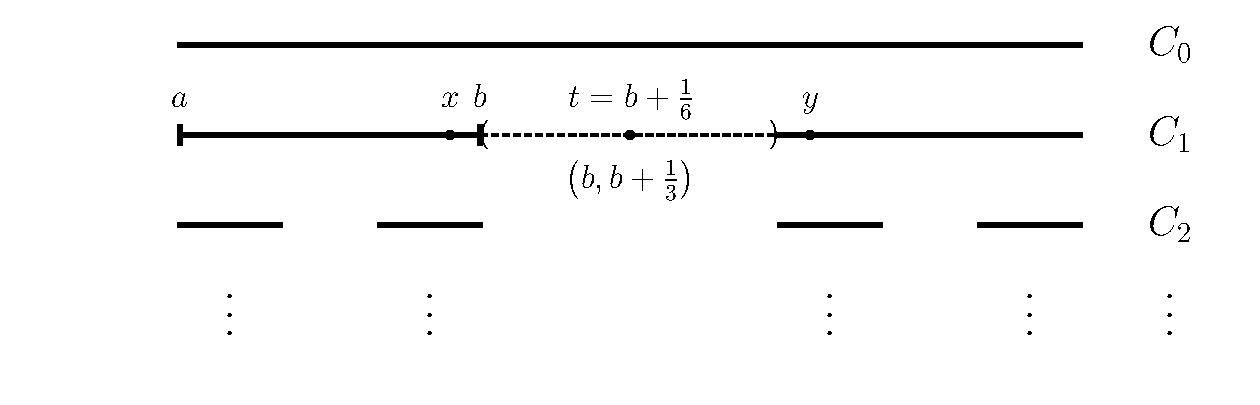
\includegraphics[width=\textwidth]{UA_Figures/UA_ex3_4_8_fig.pdf}
            \caption{Example construction of \( t \); here \( N = 1 \), but notice that any \( N \geq 1 \) would also work}
            \label{fig:ex3.4.8}
        \end{figure}
    \end{enumerate}
\end{solution}

\begin{exercise}
\label{ex:3.4.9}
    Let \( \{ r_1, r_2, r_3, \ldots \} \) be an enumeration of the rational numbers, and for each \( n \in \N \) set \( \epsilon_n = 1/2^n \). Define \( O = \bigcup_{n=1}^{\infty} V_{\epsilon_n}(r_n) \) and let \( F = \setcomp{O} \).
    \begin{enumerate}
        \item Argue that \( F \) is a closed, nonempty set consisting only of irrational numbers.

        \item Does \( F \) contain any nonempty open intervals? Is \( F \) totally disconnected? (See \Cref{ex:3.4.7} for the definition.)

        \item Is it possible to know whether \( F \) is perfect? If not, can we modify this construction to produce a nonempty perfect set of irrational numbers?
    \end{enumerate}
\end{exercise}

\begin{solution}
    \begin{enumerate}
        \item \( O \) is an open set since it is a union of open intervals, so \( F = \setcomp{O} \) must be closed. To see that \( F \) is non-empty, suppose otherwise, so that \( O = \R \). It follows that the collection \( \{ V_{\epsilon_n}(r_n) : n \in \N \} \) is an open cover of the compact set \( [0, 10] \). Thus, by Theorem 3.3.8, there exist finitely many indices \( n_1 < \cdots < n_K \) such that
        \[
            [0, 10] \subseteq V_{\epsilon_{n_1}}(r_{n_1}) \cup \cdots \cup V_{\epsilon_{n_K}}(r_{n_K}).
        \]
        However, the interval \( [0, 10] \) has length 10, whereas the set \( V_{\epsilon_{n_1}}(r_{n_1}) \cup \cdots \cup V_{\epsilon_{n_K}}(r_{n_K}) \) has total length at most
        \[
            \sum_{k=1}^K \frac{1}{2^{n_k - 1}} \leq \sum_{n=0}^{\infty} \frac{1}{2^n} = 2,
        \]
        since \( \abs{V_{\epsilon_{n_k}}(r_{n_k})} = 2 \epsilon_{n_k} = 2^{-n_k + 1} \). So we have a set of length 10 contained inside a set of length 2, which is a contradiction; it follows that \( F \) is non-empty. Finally, since \( \Q \subseteq O \), we see that \( F = \setcomp{O} \) can contain only irrational numbers.

        \item \( F \) cannot contain any non-empty open intervals, since this would imply that \( F \) contains a rational number (indeed, infinitely many rational numbers), but by part (a) \( F \) contains only irrational numbers.

        To see that \( F \) is totally disconnected, let us prove the following lemma.

        \begin{lemma}
        \label{lem:ex3.4.9}
            Suppose \( G \subseteq \R \) is totally disconnected. If \( E \) is a non-empty subset of \( G \), then \( E \) is also totally disconnected.
        \end{lemma}
        \begin{proof}
            Let \( x, y \in E \) be given. Since \( x \) and \( y \) belong to the totally disconnected set \( G \), there exist separated sets \( A \) and \( B \) such that \( x \in A, y \in B, \) and \( G = A \cup B \). Set \( A' = A \cap E \) and \( B' = B \cap E \) and note that \( x \in A' \) and \( y \in B' \). Furthermore, \( A' \subseteq A \) and \( B' \subseteq B \), so
            \[
                \overline{A'} \subseteq \overline{A} \implies \paren{ \, \overline{A'} \cap B' \, } \subseteq \paren{ \, \overline{A} \cap B' \, } \subseteq \paren{ \, \overline{A} \cap B \, } = \emptyset.
            \]
            Thus \( \overline{A'} \cap B' = \emptyset \), and similarly \( A' \cap \overline{B'} = \emptyset \); it follows that \( A' \) and \( B' \) are separated. Finally,
            \[
                E = E \cap G = E \cap (A \cup B) = (A \cap E) \cup (B \cap E) = A' \cup B'.
            \]
            Thus \( E \) is totally disconnected.
        \end{proof}
        
        Since \( F \) is a subset of \( \I \), which we showed was totally disconnected in \Cref{ex:3.4.7}, it follows from \Cref{lem:ex3.4.9} that \( F \) is totally disconnected.

        \item There are enumerations of \( \Q \) which, when used in this construction, will result in an \( F \) which is not perfect, i.e., an \( F \) with at least one isolated point. We will construct such an enumeration \( (r_n) \), which gives an \( F \) with \( \sqrt{2} \) as an isolated point, via the following four step process. (Any irrational number would also work in place of \( \sqrt{2} \). \href{https://math.stackexchange.com/questions/2854900/constructing-perfect-set-without-rationals-by-removing-open-neighborhood-around/2857460#2857460}{This construction is due to math.SE user Ingix}, however the exposition given here is my own; what follows is lengthy and involved.)
        \begin{description}
            \item[Step 1.] We will first construct a strictly increasing sequence \( (p_n) \) of distinct rational numbers such that:
            \begin{enumerate}[itemsep=8pt, leftmargin=44pt, label=(1.\arabic*)]
                \item \( p_1 < p_2 < p_3 < \cdots < \sqrt{2} \);

                \item \( \paren{ \sqrt{2} - \tfrac{1}{16}, \sqrt{2} } \subseteq \bigcup_{n=1}^{\infty} V_{\epsilon_{4n}}(p_n) \);

                \item \( \sqrt{2} \not\in \bigcup_{n=1}^{\infty} V_{\epsilon_{4n}}(p_n) \).
            \end{enumerate}
            This sequence will be placed in the final enumeration \( (r_n) \) as \( r_{4n} = p_n \), so that
            \[
                r_4 = p_1, r_8 = p_2, r_{12} = p_3, \ldots
            \]

            \item[Step 2.] Mirroring Step 1, we will construct a strictly decreasing sequence \( (q_n) \) of distinct rational numbers such that:
            \begin{enumerate}[itemsep=8pt, leftmargin=44pt, label=(2.\arabic*)]
                \item \( \sqrt{2} < \cdots < q_3 < q_2 < q_1 \);

                \item \( \paren{ \sqrt{2}, \sqrt{2} + \tfrac{1}{16} } \subseteq \bigcup_{n=1}^{\infty} V_{\epsilon_{4n-2}}(q_n) \);

                \item \( \sqrt{2} \not\in \bigcup_{n=1}^{\infty} V_{\epsilon_{4n-2}}(q_n) \).
            \end{enumerate}
            This sequence will be placed in the final enumeration \( (r_n) \) as \( r_{4n-2} = q_n \), so that
            \[
                r_2 = q_1, r_6 = q_2, r_{10} = q_3, \ldots
            \]

            \item[Step 3.] There are infinitely many rational numbers which belong to neither of the sequences \( (p_n) \) nor \( (q_n) \) from Steps 1 and 2. We will construct a sequence \( (a_n) \) which enumerates these remaining rational numbers in such a way that \( \sqrt{2} \) will not be excluded from \( F \) in the final construction, i.e., a sequence \( (a_n) \) such that:
            \begin{enumerate}[itemsep=8pt, leftmargin=44pt, label=(3.\arabic*)]
                \item \( a_m \neq a_n \) for \( m \neq n \);

                \item for each rational \( r \in \setcomp{(\{ p_1, p_2, \ldots \} \cup \{ q_1, q_2, \ldots \})}, \) there exists an \( n \in \N \) such that \( a_n = r \).

                \item \( \sqrt{2} \not\in \bigcup_{n=1}^{\infty} V_{\epsilon_{2n-1}}(a_n) \).
            \end{enumerate}
            This sequence will be placed in the final enumeration \( (r_n) \) as \( r_{2n-1} = a_n \), so that
            \[
                r_1 = a_1, r_3 = a_2, r_5 = a_3, \ldots
            \]

            \item[Step 4.] We will combine the sequences \( (p_n), (q_n), \) and \( (a_n) \) to obtain an enumeration \( (r_n) \) of \( \Q \) given by
            \[
                a_1, q_1, a_2, p_1, a_3, q_2, a_4, p_2, \ldots
            \]
            Letting \( O = \bigcup_{n=1}^{\infty} V_{\epsilon_n}(r_n) \) and \( F = \setcomp{O} \), we will have
            \[
                \paren{ \sqrt{2} - \tfrac{1}{16}, \sqrt{2} } \cup \paren{ \sqrt{2}, \sqrt{2} + \tfrac{1}{16} } \subseteq O \hspaceand \sqrt{2} \not\in O,
            \]
            so that \( \paren{ \sqrt{2} - \tfrac{1}{16}, \sqrt{2} + \tfrac{1}{16} } \cap F = \set{ \sqrt{2} } \). Thus \( \sqrt{2} \) will be an isolated point of \( F \).
        \end{description}

        \noindent \hrulefill

        \noindent {\Large \textbf{Step 1.}}

        \noindent For each \( n \in \N \), let \( p_n \) be a rational number satisfying
        \[
            \sqrt{2} - \frac{1}{2^{4n}} - \frac{1}{2^{4n + 4}} < p_n < \sqrt{2} - \frac{1}{2^{4n}} < \sqrt{2};
        \]
        the existence of such a rational number is guaranteed by the density of \( \Q \) in \( \R \). From this definition, it is straightforward to verify that the sequence \( (p_n) \) satisfies condition (1.1). Observe that for any \( n \in \N \) we have
        \[
            p_n < p_{n+1} < p_n + \frac{1}{2^{4n}} < \sqrt{2};
        \]
        it follows that \( \sqrt{2} \not\in V_{\epsilon_{4n}}(p_n) \) for each \( n \in \N \), so that the sequence \( (p_n) \) satisfies condition (1.3). Furthermore, \( p_{n+1} \in \paren{ p_n, p_n + 2^{-4n} } \subseteq V_{\epsilon_{4n}}(p_n) \), i.e., the centre of \( V_{\epsilon_{4n+4}}(p_{n+1}) \) is contained in \( V_{\epsilon_{4n}}(p_n) \). Thus, for any \( N \in \N \), the union \( \bigcup_{n=1}^N V_{\epsilon_{4n}}(p_n) \) must be an open interval:
        \[
            \bigcup_{n=1}^N V_{\epsilon_{4n}}(p_n) = \paren{ p_1 - \frac{1}{16}, B },
        \]
        where \( B = \max \{ p_n + 2^{-4n} : 1 \leq n \leq N \} \) (the exact value of \( B \) is not important, but note that it must be strictly less than \( \sqrt{2} \)). Since
        \[
            \sqrt{2} - \frac{1}{16} \in \paren{ p_1 - \frac{1}{16}, p_1 + \frac{1}{16} } = V_{\epsilon_4}(p_1),
        \]
        we have \( \sqrt{2} - \tfrac{1}{16} \in \bigcup_{n=1}^N V_{\epsilon_{4n}}(p_n) \) for any \( N \in \N \). Let \( y \in \R \) be such that \( \sqrt{2} - \tfrac{1}{16} < y < \sqrt{2} \). Because \( (p_n) \) converges to \( \sqrt{2} \) (by the Squeeze Theorem), we can find an \( N \in \N \) such that \( y < p_N < \sqrt{2} \). It follows that \( \sqrt{2} - \tfrac{1}{16} \) and \( p_N \) both belong to the open interval \( \bigcup_{n=1}^N V_{\epsilon_{4n}}(p_n) \); since \( y \) lies between these two values, we must then have \( y \in \bigcup_{n=1}^N V_{\epsilon_{4n}}(p_n) \subseteq \bigcup_{n=1}^{\infty} V_{\epsilon_{4n}}(p_n) \). Thus the sequence \( (p_n) \) satisfies condition (1.2).

        \noindent \hrulefill

        \noindent {\Large \textbf{Step 2.}}

        \noindent The construction of the sequence \( (q_n) \) is analogous to the construction given in Step 1; for each \( n \in \N \), let \( q_n \) be a rational number satisfying
        \[
            \sqrt{2} + \frac{1}{2^{4n - 2}} < q_n <  \sqrt{2} + \frac{1}{2^{4n - 2}} + \frac{1}{2^{4n + 2}}.
        \]
        Arguing as in Step 1, we see that the sequence \( (q_n) \) satisfies condition (2.1), and furthermore that \( \paren{ \sqrt{2}, \sqrt{2} + \tfrac{1}{4} } \subseteq \bigcup_{n=1}^{\infty} V_{\epsilon_{4n-2}}(q_n) \), which gives us condition (2.2). Condition (2.3) follows since \( \sqrt{2} < q_n - \tfrac{1}{2^{4n - 2}} \) for all \( n \in \N \).

        \noindent \hrulefill

        \noindent {\Large \textbf{Step 3.}}

        \noindent Since the sequences \( (p_n) \) and \( (q_n) \) constructed in Steps 1 and 2 are entirely contained inside the interval \( [p_1, q_1] \), we still have infinitely many rational numbers left to enumerate. That is, letting
        \[
            E = \Q \cap \setcomp{(\{ p_1, p_2, \ldots \} \cup \{ q_1, q_2, \ldots \})},
        \]
        we have that \( E \) is countably infinite. However, enumerating \( E \) carelessly might exclude \( \sqrt{2}\) from \( F \) in Step 4, since there are rational numbers in \( E \) arbitrarily close to \( \sqrt{2} \); placing one of these rational numbers ``too early'' in the sequence \( (r_n) \) will include \( \sqrt{2} \) in some \( V_{\epsilon_n}(r_n) \). To surmount this problem, we will first partition \( E \) as follows. Let
        \[
            A_n = \begin{cases}
                \set{ x \in \R : \epsilon_1 < \abs{x - \sqrt{2}} } & \text{if } n = 1, \\
                \set{ x \in \R : \epsilon_{2n - 1} < \abs{x - \sqrt{2}} < \epsilon_{2n - 3} } & \text{if } n \geq 2.
            \end{cases}
        \]
        Equivalently,
        \[
            A_n = \begin{cases}
                \paren{ -\infty, \sqrt{2} - \epsilon_1 } \cup \paren{ \sqrt{2} + \epsilon_1, \infty } & \text{if } n = 1, \\
                \paren{ \sqrt{2} - \epsilon_{2n - 3}, \sqrt{2} - \epsilon_{2n - 1} } \cup \paren{ \sqrt{2} + \epsilon_{2n - 1}, \sqrt{2} + \epsilon_{2n - 3} } & \text{if } n \geq 2.
            \end{cases}
        \]
        Now set \( E_n = E \cap A_n \) for each \( n \in \N \).
        \begin{center}
            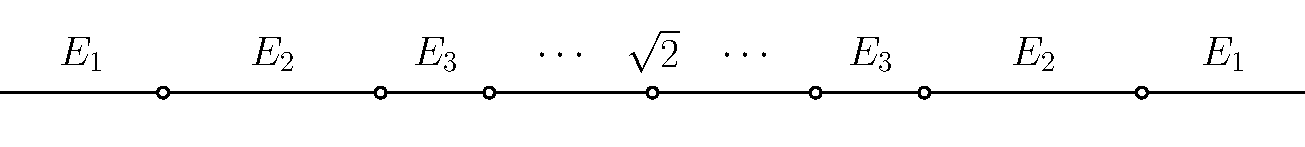
\includegraphics[width=0.8\textwidth]{UA_Figures/UA_ex3_4_9_fig_1.pdf}
        \end{center}
        
        We have \( \bigcup_{n=1}^{\infty} E_n = E \) since the only real numbers not contained in \( \bigcup_{n=1}^{\infty} A_n \) are \( \sqrt{2} \) and those of the form \( \sqrt{2} \pm \epsilon_{2n - 1} \) for some \( n \in \N \), none of which are rational, and the collection \( \{ E_n : n \in \N \} \) is evidently pairwise disjoint; it follows that this collection is a partition of \( E \).

        Since \( \lim_{n \to \infty} p_n = \lim_{n \to \infty} q_n = \sqrt{2} \) and \( \sqrt{2} \not\in \overline{A_n} \) for any \( n \in \N \), we see that there can be only finitely many terms of the sequences \( (p_n) \) and \( (q_n) \) contained in each \( A_n \); it follows that each \( E_n \) is countably infinite. We can then enumerate each \( E_n \):
        \[
            E_n = \{ e_{1,n}, e_{2,n}, e_{3,n}, \ldots \}.
        \]
        These enumerations can be combined to form an enumeration \( (a_n) \) of \( E \) using the same method of the proof that a countable union of countable sets is itself countable (see, for example, \Cref{ex:1.5.3} (c)). To be precise, consider the following ``infinite arrays''.
        \[
            \begin{array}{cccccc}
                E_1 & E_2 & E_3 & E_4 & E_5 & \cdots \\
                \hline
                e_{1,1} & e_{1,2} & e_{1,3} & e_{1,4} & e_{1,5} & \cdots \\[2mm]
                e_{2,1} & e_{2,2} & e_{2,3} & e_{2,4} & e_{2,5} & \cdots \\[2mm]
                e_{3,1} & e_{3,2} & e_{3,3} & e_{3,4} & e_{3,5} & \cdots \\[2mm]
                e_{4,1} & e_{4,2} & e_{4,3} & e_{4,4} & e_{4,5} & \cdots \\[2mm]
                e_{5,1} & e_{5,2} & e_{5,3} & e_{5,4} & e_{5,5} & \cdots \\[2mm]
                \vdots & \vdots & \vdots & \vdots & \vdots & \ddots
            \end{array}
            \qquad
            \begin{array}{cccccc}
                1 & 2 & 3 & 4 & 5 & \cdots \\
                \hline
                a_1 & a_3 & a_6 & a_{10} & a_{15} & \cdots \\[2mm]
                a_2 & a_5 & a_9 & a_{14} & a_{20} & \cdots \\[2mm]
                a_4 & a_8 & a_{13} & a_{19} & a_{26} & \cdots \\[2mm]
                a_7 & a_{12} & a_{18} & a_{25} & a_{33} & \cdots \\[2mm]
                a_{11} & a_{17} & a_{24} & a_{32} & a_{41} & \cdots \\[2mm]
                \vdots & \vdots & \vdots & \vdots & \vdots & \ddots
            \end{array}
        \]
        The enumeration of \( E_n \) is the \( n \)\ts{th} column of the left-hand array. The enumeration of \( E \) is obtained by letting \( a_N \) in the right-hand array be the element \( e_{m,n} \) in the corresponding position of the left-hand array, so that
        \[
            a_1 = e_{1,1}, a_2 = e_{2,1}, a_3 = e_{1,2}, a_4 = e_{3,1}, \ldots
        \]
        This mapping is bijective because the collection \( \{ E_n : n \in \N \} \) is a partition of \( E \) and thus the sequence \( (a_n) \) satisfies conditions (3.1) and (3.2).

        To show that the sequence \( (a_n) \) satisfies condition (3.3), we need to show that for all \( n \in \N, \sqrt{2} \not\in V_{\epsilon_{2n - 1}}(a_n) \). Let \( n \in \N \) be given. The element \( a_n \) belongs to some column of the right-hand array above, say the \( N \)\ts{th} column. From the definition of our enumeration \( (a_n) \), we have \( a_n = e_{m,N} \) for some \( m \in \N \). It follows that \( a_n \in E_N \) and hence that \( \abs{a_n - \sqrt{2}} > \epsilon_{2N - 1} \), which gives \( \sqrt{2} \not\in V_{\epsilon_{2N - 1}}(a_n) \).
        
        If we examine the right-hand array, we see that the element at the top of the \( N \)\ts{th} column is \( a_{N(N+1)/2} \) (the \( N \)\ts{th} triangular number), and furthermore that \( n \geq N(N+1)/2 \). Thus
        \[
            2n - 1 \geq 2N - 1 \implies \epsilon_{2n-1} \leq \epsilon_{2N-1} \implies V_{\epsilon_{2n - 1}}(a_n) \subseteq V_{\epsilon_{2N - 1}}(a_n).
        \]
        Combining this with \( \sqrt{2} \not\in V_{\epsilon_{2N - 1}}(a_n) \), we see that \( \sqrt{2} \not\in V_{\epsilon_{2n - 1}}(a_n) \); it follows that the sequence \( (a_n) \) satisfies condition (3.3).

        \noindent \hrulefill

        \noindent {\Large \textbf{Step 4.}}

        \noindent We can now form our final enumeration \( (r_n) \), by letting
        \[
            r_{2n-1} = a_n, \quad r_{4n-2} = q_n, \hspaceand r_{4n} = p_n,
        \]
        so that \( (r_n) \) is the sequence
        \[
            a_1, q_1, a_2, p_1, a_3, q_2, a_4, p_2, \ldots
        \]
        Let \( O = \bigcup_{n=1}^{\infty} V_{\epsilon_n}(r_n) \) and \( F = \setcomp{O} \). By condition (1.2), we have
        \[
            \paren{ \sqrt{2} - \frac{1}{16}, \sqrt{2} } \subseteq \bigcup_{n=1}^{\infty} V_{\epsilon_{4n}}(p_n) = \bigcup_{n=1}^{\infty} V_{\epsilon_{4n}}(r_{4n}) \subseteq \bigcup_{n=1}^{\infty} V_{\epsilon_n}(r_n) = O,
        \]
        and by condition (2.2), we have
        \[
            \paren{ \sqrt{2}, \sqrt{2} + \frac{1}{16} } \subseteq \bigcup_{n=1}^{\infty} V_{\epsilon_{4n-2}}(q_n) = \bigcup_{n=1}^{\infty} V_{\epsilon_{4n-2}}(r_{4n-2}) \subseteq \bigcup_{n=1}^{\infty} V_{\epsilon_n}(r_n) = O.
        \]
        Thus \( \paren{ \sqrt{2} - \tfrac{1}{16}, \sqrt{2} } \cup \paren{ \sqrt{2}, \sqrt{2} + \tfrac{1}{16} } \subseteq O \). Furthermore, since
        \begin{align*}
            O &= \bigcup_{n=1}^{\infty} V_{\epsilon_n}(r_n) \\[2mm]
            &= \bigcup_{n=1}^{\infty} V_{\epsilon_{4n}}(r_{4n}) \cup \bigcup_{n=1}^{\infty} V_{\epsilon_{4n-2}}(r_{4n-2}) \cup \bigcup_{n=1}^{\infty} V_{\epsilon_{2n-1}}(r_{2n-1}) \\[2mm]
            &= \bigcup_{n=1}^{\infty} V_{\epsilon_{4n}}(p_n) \cup \bigcup_{n=1}^{\infty} V_{\epsilon_{4n-2}}(q_n) \cup \bigcup_{n=1}^{\infty} V_{\epsilon_{2n-1}}(a_n),
        \end{align*}
        conditions (1.3), (2.3), and (3.3) imply that \( \sqrt{2} \not\in O \). It follows that
        \[
            \paren{ \sqrt{2} - \frac{1}{16}, \sqrt{2} + \frac{1}{16} } \cap F = \set{ \sqrt{2} },
        \]
        so that \( \sqrt{2} \) is an isolated point of \( F \). We may conclude that \( F \) is not a perfect set.

        \noindent \hrulefill

        \noindent Regarding the second half of the question, it is possible to modify the construction to produce a non-empty perfect set consisting of only irrational numbers. To do this, we start with any enumeration \( (r_n) \) of \( \Q \) and recursively define a sequence of non-negative real numbers \( (\epsilon_n) \) in such a way that if we set
        \[
            O = \bigcup_{n=1}^{\infty} V_{\epsilon_n}(r_n) \hspaceand F = \setcomp{O},
        \]
        then \( F \) will be a non-empty perfect of irrational numbers. Intuitively, we will recursively construct \( O \) as a union of disjoint open intervals, with no pair of these intervals sharing an endpoint. (In what follows, we adopt the convention that \( V_{\epsilon}(x) = \emptyset \) if \( \epsilon = 0 \).)

        Suppose that after \( N \) steps we have chosen \( \epsilon_1, \ldots, \epsilon_N \) such that:
        \begin{enumerate}[leftmargin=40pt, label=(IH\arabic*)]
            \item \( \{ r_1, \ldots, r_N \} \subseteq \bigcup_{n=1}^{N} V_{\epsilon_n}(r_n) \);

            \item for all \( 1 \leq n \leq N \), either \( \epsilon_n = 0 \) or \( \epsilon_n \) is positive, irrational, and satisfies \( \epsilon_n \leq \tfrac{\sqrt{2}}{2^n} \);

            \item \( \overline{V_{\epsilon_m}(r_m)} \cap \overline{V_{\epsilon_n}(r_n)} = \emptyset \) for all \( m, n \in \N \) with \( 1 \leq m < n \leq N \).
        \end{enumerate}
        
        Let \( U = \bigcup_{n=1}^N V_{\epsilon_n}(r_n) \). There are two cases.
        \begin{description}
            \item[Case 1.] This is the easier case. If \( r_{N+1} \in U \), then let \( \epsilon_{N+1} = 0 \), so that \( V_{\epsilon_{N+1}}(r_{N+1}) = \emptyset \). (IH1) combined with \( r_{N+1} \in U \) gives us
            \[
                \{ r_1, \ldots, r_N, r_{N+1} \} \subseteq U = \bigcup_{n=1}^N V_{\epsilon_n}(r_n) = \bigcup_{n=1}^{N+1} V_{\epsilon_n}(r_n),
            \]
            where the last equality follows because \( V_{\epsilon_{N+1}}(r_{N+1}) = \emptyset \).
            
            Combining (IH2) with \( \epsilon_{N+1} = 0 \), we see that for all \( 1 \leq n \leq N + 1 \), either \( \epsilon_n = 0 \) or \( \epsilon_n \) is positive, irrational, and satisfies \( \epsilon_n \leq \tfrac{\sqrt{2}}{2^n} \).

            Similarly, combining (IH3) with \( V_{\epsilon_{N+1}}(r_{N+1}) = \emptyset \), we have \( \overline{V_{\epsilon_m}(r_m)} \cap \overline{V_{\epsilon_n}(r_n)} = \emptyset \) for all \( m, n \in \N \) with \( 1 \leq m < n \leq N + 1 \).

            \item[Case 2.] This is the harder case. If \( r_{N+1} \not\in U \) then let \( \epsilon_{n_1}, \ldots, \epsilon_{n_J} \) be those \( \epsilon \)'s from \( \epsilon_1, \ldots, \epsilon_N \) which are non-zero; there must be at least one such \( \epsilon_{n_j} \) by (IH1) and each \( \epsilon_{n_j} \) must be positive and irrational by (IH2). Observe that
            \[
                U = \bigcup_{n=1}^N V_{\epsilon_n}(r_n) = \bigcup_{j=1}^J V_{\epsilon_{n_j}}(r_{n_j}),
            \]
            where each \( V_{\epsilon_{n_j}}(r_{n_j}) \) is a proper open interval. For each \( 1 \leq j \leq J \), note that since \( r_{N+1} \not\in U \), we must have \( r_{N+1} \not\in V_{\epsilon_{n_j}}(r_{n_j}) \). Both of the endpoints of \( V_{\epsilon_{n_j}}(r_{n_j}) \) are the sum of a rational number and an irrational number and hence are irrational; since \( r_{N+1} \) is rational, we see that \( r_{N+1} \not\in [r_{n_j} - \epsilon_{n_j}, r_{n_j} + \epsilon_{n_j}] \). Given this, if we let \( d \) be the minimum of the distances from \( r_{N+1} \) to the endpoints of each \( V_{\epsilon_{n_j}} \), i.e.,
            \[
                d = \min \set{ \abs{r_{n_j} - \epsilon_{n_j} - r_{N+1}}, \abs{r_{n_j} + \epsilon_{n_j} - r_{N+1}} : 1 \leq j \leq J },
            \]
            then \( d \) must be positive. Furthermore, \( d \) must be irrational since it is the sum of a rational number and an irrational number, and for each \( 1 \leq j \leq J \), we have
            \[
                \bkt{ r_{N+1} - \tfrac{d}{2}, r_{N+1} + \tfrac{d}{2} } \cap [r_{n_j} - \epsilon_{n_j}, r_{n_j} + \epsilon_{n_j}] = \emptyset. \tag{\dag}
            \]

            Let \( \epsilon_{N+1} = \min \set{ \tfrac{\sqrt{2}}{2^{N+1}}, \tfrac{d}{2} } \) and note that \( \epsilon_{N+1} \) is positive, so that \( r_{N+1} \in V_{\epsilon_{N+1}}(r_{N+1}) \). Combining this with (IH1) gives us
            \[
                \{ r_1, \ldots, r_N, r_{N+1} \} \subseteq \bigcup_{n=1}^{N+1} V_{\epsilon_n}(r_n).
            \]
            As noted before, \( d \) is positive and irrational, so \( \epsilon_{N+1} \) is positive, irrational, and satisfies \( \epsilon_{N+1} \leq \tfrac{\sqrt{2}}{2^{N+1}} \); combining this with (IH2) shows that for all \( 1 \leq n \leq N + 1 \), either \( \epsilon_n = 0 \) or \( \epsilon_n \) is positive, irrational, and satisfies \( \epsilon_n \leq \tfrac{\sqrt{2}}{2^n} \).

            Let \( 1 \leq n \leq N \) be given. If \( \epsilon_n = 0 \), then the identity \( \overline{V_{\epsilon_n}(r_n)} \cap \overline{V_{\epsilon_{N+1}}(r_{N+1})} = \emptyset \) is clear, since \( V_{\epsilon_n}(r_n) = \emptyset \). If \( \epsilon_n \neq 0 \), then \( n = n_j \) for some \( 1 \leq j \leq J \). In this case, we have
            \begin{multline*}
                \overline{V_{\epsilon_n}(r_n)} = \overline{V_{\epsilon_{n_j}}(r_{n_j})} = [r_{n_j} - \epsilon_{n_j}, r_{n_j} + \epsilon_{n_j}] \quad \text{and} \\[2mm]
                \overline{V_{\epsilon_{N+1}}(r_{N+1})} = [r_{N+1} - \epsilon_{N+1}, r_{N+1} + \epsilon_{N+1}] \subseteq \bkt{ r_{N+1} - \tfrac{d}{2}, r_{N+1} + \tfrac{d}{2} }.
            \end{multline*}
            By equation \( (\dag) \), we see that \( \overline{V_{\epsilon_n}(r_n)} \cap \overline{V_{\epsilon_{N+1}}(r_{N+1})} = \emptyset \). Combining this with (IH3), we see that \( \overline{V_{\epsilon_m}(r_m)} \cap \overline{V_{\epsilon_n}(r_n)} = \emptyset \) for all \( m, n \in \N \) with \( 1 \leq m < n \leq N + 1 \).
        \end{description}
        This completes the recursive step; for the base case, simply let \( \epsilon_1 = \tfrac{\sqrt{2}}{2} \). Thus we obtain a sequence \( (\epsilon_n) \) which satisfies (IH1), (IH2), and (IH3) for all \( N \in \N \). In other words, the sequence \( (\epsilon_n) \) has the following properties:
        \begin{enumerate}[itemsep=8pt, leftmargin=44pt, label=(A\arabic*)]
            \item \( \Q \subseteq \bigcup_{n=1}^{\infty} V_{\epsilon_n}(r_n) \);

            \item for all \( n \in \N \), either \( \epsilon_n = 0 \) or \( \epsilon_n \) is positive, irrational, and satisfies \( \epsilon_n \leq \tfrac{\sqrt{2}}{2^n} \);

            \item \( \overline{V_{\epsilon_m}(r_m)} \cap \overline{V_{\epsilon_n}(r_n)} = \emptyset \) for all \( m, n \in \N \) with \( m < n \).
        \end{enumerate}
        Let \( O = \bigcup_{n=1}^{\infty} V_{\epsilon_n}(r_n) \) and \( F = \setcomp{O} \). As in part (a), \( F \) is closed and, by (A1), consists solely of irrational numbers. By (A2), we have \( \epsilon_n \leq \tfrac{\sqrt{2}}{2^n} \) for each \( n \in \N \); a similar argument as in part (a) shows that \( O \) cannot be the entire real line and thus \( F \) is non-empty.
        
        To see that \( F \) is perfect, suppose by way of contradiction that \( x \in F \) is isolated, i.e., there exists a \( \delta > 0 \) such that \( (x - \delta, x + \delta) \cap F = \{ x \} \). This implies that the intervals \( (x - \delta, x) \) and \( (x, x + \delta) \) are contained in \( O \). We claim that if an interval such as \( (x - \delta, x) \) is to be contained in \( O \), then it must be entirely contained inside a single \( V_{\epsilon_n}(r_n) \). To see this, suppose by way of contradiction that \( a, b \in (x - \delta, x) \) are such that \( a < b, a \in V_{\epsilon_m}(r_m), \) and \( b \in V_{\epsilon_n}(r_n) \), with \( m \neq n \). By (A3), it must then be the case that
        \[
            a < r_m + \epsilon_m < r_n - \epsilon_n < b.
        \]
        \begin{center}
            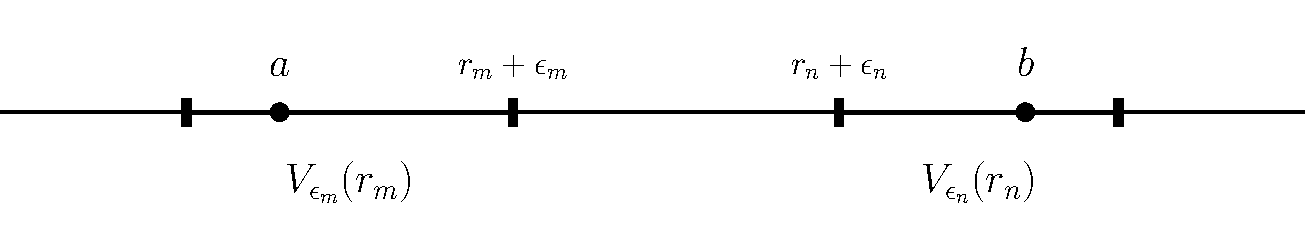
\includegraphics[width=0.9\textwidth]{UA_Figures/UA_ex3_4_9_fig_2.pdf}
        \end{center}
        So \( r_m + \epsilon_m \in (a, b) \subseteq (x - \delta, x) \subseteq O = \bigcup_{n=1}^{\infty} V_{\epsilon_n}(r_n) \); it follows that there exists a \( k \in \N \) such that \( r_m + \epsilon_m \) belongs to \( V_{\epsilon_k}(r_k) \). If \( k = m \), this says that an open interval contains one of its endpoints, and if \( k \neq m \) then this violates (A3). In either case, we have a contradiction.

        Thus if an interval such as \( (x - \delta, x) \) is to be contained in \( O \), it must be entirely contained inside a single \( V_{\epsilon_n}(r_n) \). Since \( (x - \delta, x) \) and \( (x, x + \delta) \) are disjoint, there exist positive integers \( m \neq n \) such that
        \[
            (x - \delta, x) \subseteq V_{\epsilon_m}(r_m) \hspaceand (x, x + \delta) \subseteq V_{\epsilon_n}(r_n).
        \]
        This implies that
        \[
            [x - \delta, x] \subseteq \overline{V_{\epsilon_m}(r_m)} \hspaceand[8mm] [x, x + \delta] \subseteq \overline{V_{\epsilon_n}(r_n)},
        \]
        which in turn gives \( x \in \overline{V_{\epsilon_m}(r_m)} \cap \overline{V_{\epsilon_n}(r_n)} \), contradicting (A3). We may conclude that \( F \) is a perfect set.
    \end{enumerate}
\end{solution}

\section{Baire's Theorem}
\label{sec:3.5}

\begin{exercise}
\label{ex:3.5.1}
    Argue that a set \( A \) is a \( G_{\delta} \) set if and only if its complement is an \( F_{\sigma} \) set.
\end{exercise}

\begin{solution}
    This is immediate from De Morgan's Laws (see \Cref{ex:3.2.9}).
\end{solution}

\begin{exercise}
\label{ex:3.5.2}
    Replace each \rule{1cm}{0.15mm} with the word \textit{finite} or \textit{countable} depending on which is more appropriate.
    \begin{enumerate}
        \item The \rule{1cm}{0.15mm} union of \( F_{\sigma} \) sets is an \( F_{\sigma} \) set.

        \item The \rule{1cm}{0.15mm} intersection of \( F_{\sigma} \) sets is an \( F_{\sigma} \) set.

        \item The \rule{1cm}{0.15mm} union of \( G_{\delta} \) sets is a \( G_{\delta} \) set.

        \item The \rule{1cm}{0.15mm} intersection of \( G_{\delta} \) sets is a \( G_{\delta} \) set.
    \end{enumerate}
\end{exercise}

\begin{solution}
    \begin{enumerate}
        \item The countable union of \( F_{\sigma} \) sets is an \( F_{\sigma} \) set. Suppose we have a countable collection \( \{ A_m : m \in \N \} \) of \( F_{\sigma} \) sets, i.e., for each \( m \in \N \) there is a countable collection \( \{ B_{m,n} : n \in \N \} \) of closed sets such that \( A_m = \bigcup_{n=1}^{\infty} B_{m,n} \). Notice that
        \[
            \bigcup_{m=1}^{\infty} A_m = \bigcup_{m=1}^{\infty} \bigcup_{n=1}^{\infty} B_{m,n} = \bigcup_{(m, n) \in \N^2} B_{m,n}.
        \]
        Since \( \N^2 \) is countable (\Cref{lem:ex1.5.9}), we have expressed \( \bigcup_{m=1}^{\infty} A_m \) as a countable union of closed sets; it follows that \( \bigcup_{m=1}^{\infty} A_m \) is an \( F_{\sigma} \) set.

        \item The finite intersection of \( F_{\sigma} \) sets is an \( F_{\sigma} \) set. To see this, it will suffice to show that if \( A \) and \( B \) are \( F_{\sigma} \) sets, then \( A \cap B \) is an \( F_{\sigma} \) set; the general case will then follow from a straightforward induction argument. Suppose therefore that \( A = \bigcup_{m=1}^{\infty} A_m \) and \( B = \bigcup_{n=1}^{\infty} B_n \), where \( \{ A_m : m \in \N \} \) and \( \{ B_n : n \in \N \} \) are countable collections of closed sets, and observe that
        \[
            A \cap B = \paren{ \bigcup_{m=1}^{\infty} A_m } \cap \paren{ \bigcup_{n=1}^{\infty} B_n } = \bigcup_{(m, n) \in \N^2} (A_m \cap B_n).
        \]
        Since each \( A_m \cap B_n \) is closed (being an intersection of closed sets) and \( \N^2 \) is countable (\Cref{lem:ex1.5.9}), we have expressed \( A \cap B \) as a countable union of closed sets; it follows that \( A \cap B \) is an \( F_{\sigma} \) set.

        The countable intersection of \( F_{\sigma} \) sets need not be an \( F_{\sigma} \) set. For a counterexample, let \( \{ r_1, r_2, \ldots \} \) be an enumeration of \( \Q \) and for positive integers \( m, n \), let
        \[
            B_{m, n} := \left( -\infty, r_m - \frac{1}{n} \right] \cup \left[ r_m + \frac{1}{n}, \infty \right).
        \]
        Each \( B_{m, n} \) is a closed set, so if we let \( A_m := \bigcup_{n=1}^{\infty} B_{m, n} \) for each \( m \in \N \), then each \( A_m \) is an \( F_{\sigma} \) set. We claim that \( \bigcap_{m=1}^{\infty} A_m = \I \), the set of irrational numbers. To see this, we will show that \( \setcomp{(\bigcap_{m=1}^{\infty} A_m)} = \Q \). By De Morgan's Laws (\Cref{ex:3.2.9}), we have
        \begin{multline*}
            \setcomp{\paren{ \bigcap_{m=1}^{\infty} A_m }} = \bigcup_{m=1}^{\infty} \setcomp{A_m} = \bigcup_{m=1}^{\infty} \setcomp{\paren{ \bigcup_{n=1}^{\infty} B_{m, n} }} \\[4mm]
            = \bigcup_{m=1}^{\infty} \bigcap_{n=1}^{\infty} \setcomp{B_{m, n}} = \bigcup_{m=1}^{\infty} \bigcap_{n=1}^{\infty} \paren{ r_m - \frac{1}{n}, r_m + \frac{1}{n} } = \bigcup_{m=1}^{\infty} \{ r_m \} = \Q.
        \end{multline*}
        Thus \( \bigcap_{m=1}^{\infty} A_m = \I \). As we will show in \Cref{ex:3.5.6}, \( \I \) is not an \( F_{\sigma} \) set.

        \item The finite union of \( G_{\delta} \) sets is a \( G_{\delta} \) set, but the countable union of \( G_{\delta} \) sets need not be a \( G_{\delta} \) set; these statements follow from part (b) of this exercise, \Cref{ex:3.5.1}, and De Morgan's Laws (\Cref{ex:3.2.9}).

        \item The countable intersection of \( G_{\delta} \) sets is a \( G_{\delta} \) set. Again, this follows from part (a) of this exercise, \Cref{ex:3.5.1}, and De Morgan's Laws (\Cref{ex:3.2.9}).
    \end{enumerate}
\end{solution}

\begin{exercise}
\label{ex:3.5.3}
    (This exercise has already appeared as \Cref{ex:3.2.15}.)
    \begin{enumerate}
        \item Show that a closed interval \( [a, b] \) is a \( G_{\delta} \) set.
        
        \item Show that the half-open interval \( (a, b] \) is both a \( G_{\delta} \) and an \( F_{\sigma} \) set.

        \item Show that \( \Q \) is an \( F_{\sigma} \) set, and the set of irrationals \( \I \) forms a \( G_{\delta} \) set.
    \end{enumerate}
\end{exercise}

\begin{solution}
    See \Cref{ex:3.2.15}.
\end{solution}

\begin{exercise}
\label{ex:3.5.4}
    Starting with \( n = 1 \), inductively construct a nested sequence of \textit{closed} intervals \( I_1 \supseteq I_2 \supseteq I_3 \supseteq \cdots \) satisfying \( I_n \subseteq G_n \). Give special attention to the issue of the endpoints of each \( I_n \). Show how this leads to a proof of the theorem.
\end{exercise}

\begin{solution}
    Since \( G_1 \) is dense, it must be non-empty, i.e., there exists some \( x_1 \in G_1 \), and then since \( G_1 \) is open there exists an \( \epsilon_1 > 0 \) such that \( (x_1 - \epsilon_1, x_1 + \epsilon_1) \subseteq G_1 \). Let
    \[
        a_1 := x_1 - \frac{\epsilon_1}{2}, \qquad b_1 := x_1 + \frac{\epsilon_1}{2}, \hspaceand I_1 := [a_1, b_1],
    \]
    and note that \( I_1 \subseteq (x_1 - \epsilon_1, x_1 + \epsilon_1) \subseteq G_1 \). This handles the base case.
    
    \begin{center}
        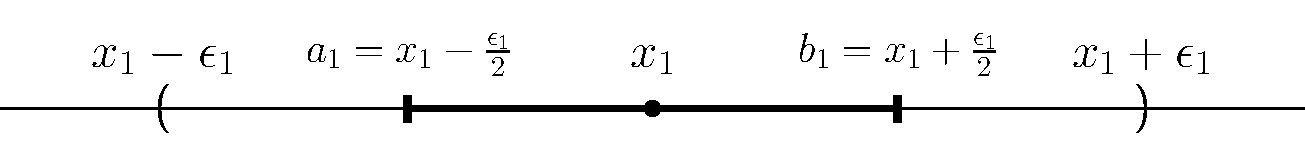
\includegraphics[width=0.9\textwidth]{UA_Figures/UA_ex3_5_4_fig.pdf}
    \end{center}

    Suppose that after \( n \) steps we have chosen nested, closed intervals \( I_1 = [a_1, b_1] \supseteq \cdots \supseteq I_n = [a_n, b_n] \) such that \( I_1 \subseteq G_1, \ldots, I_n \subseteq G_n \) and \( a_1 < b_1, \ldots, a_n < b_n \). Since \( G_{n+1} \) is dense, there exists some \( x_{n+1} \in G_{n+1} \) such that \( a_n < x_{n+1} < b_n \), and since \( G_{n+1} \) is open there exists some \( \epsilon_{n+1} > 0 \) such that \( (x_{n+1} - \epsilon_{n+1}, x_{n+1} + \epsilon_{n+1}) \subseteq G_{n+1} \). Let \( \delta = \min \set{ \tfrac{\epsilon_{n+1}}{2}, x_{n+1} - a_n, b_n - x_{n+1} } \), and define
    \[
        a_{n+1} := x_{n+1} - \delta, \qquad b_{n+1} := x_{n+1} + \delta, \hspaceand I_{n+1} := [a_{n+1}, b_{n+1}].
    \]
    Note that \( a_{n+1} < b_{n+1} \), and since \( \delta \leq x_{n+1} - a_n \) and \( \delta \leq b_n - x_{n+1} \), we have \( I_{n+1} \subseteq I_n \). Moreover, because \( \delta \leq \tfrac{\epsilon_{n+1}}{2} \), we also have \( I_{n+1} \subseteq (x_{n+1} - \epsilon_{n+1}, x_{n+1} + \epsilon_{n+1}) \subseteq G_{n+1} \). This completes the induction step.

    We then obtain a nested sequence of closed intervals \( (I_n)_{n=1}^{\infty} \) such that \( I_n \subseteq G_n \) for each \( n \in \N \). We may now appeal to the Nested Interval Property (Theorem 1.4.1) to obtain some \( x \in \bigcap_{n=1}^{\infty} I_n \), which must also belong to \( \bigcap_{n=1}^{\infty} G_n \).
\end{solution}

\begin{exercise}
\label{ex:3.5.5}
    Show that it is impossible to write
    \[
        \R = \bigcup_{n=1}^{\infty} F_n,
    \]
    where for each \( n \in \N, F_n \) is a closed set containing no nonempty open intervals.
\end{exercise}

\begin{solution}
    Suppose that \( \{ F_n : n \in \N \} \) is a collection of closed sets, each of which contains no non-empty open intervals. Let \( n \in \N \) be given and let \( x < z \) be arbitrary real numbers. By assumption \( (x, z) \not\subseteq F_n \), so there must exist some \( y \in (x, z) \cap \setcomp{F_n} \); it follows that \( \setcomp{F_n} \) is dense.

    Thus \( \{ \setcomp{F_n} : n \in \N \} \) is a collection of open, dense sets. Theorem 3.5.2 (\Cref{ex:3.5.4}) and De Morgan's Laws (\Cref{ex:3.2.9}) now imply that
    \[
        \bigcap_{n=1}^{\infty} \setcomp{F_n} \neq \emptyset \iff \bigcup_{n=1}^{\infty} F_n \neq \R.
    \]
\end{solution}

\begin{exercise}
\label{ex:3.5.6}
    Show how the previous exercise implies that the set \( \I \) of irrationals cannot be an \( F_{\sigma} \) set, and \( \Q \) cannot be a \( G_{\delta} \) set.
\end{exercise}

\begin{solution}
    We will argue by contradiction. Suppose that \( \I \) is an \( F_{\sigma} \) set, so that \( \I = \bigcup_{m=1}^{\infty} F_m \), where each \( F_m \) is closed. Note that for any \( m \in \N \), it must be the case that \( F_m \) contains no non-empty open interval; otherwise, \( F_m \) would contain infinitely many rational numbers. Let \( \{ r_1, r_2, \ldots \} \) be an enumeration of \( \Q \), so that \( \Q = \bigcup_{n=1}^{\infty} \{ r_n \} \), and note that each singleton \( \{ r_n \} \) is closed and contains no non-empty interval. Observe that
    \[
        \R = \I \cup \Q = \paren{ \bigcup_{m=1}^{\infty} F_m } \cup \paren{ \bigcup_{n=1}^{\infty} \{ r_n \} } = \bigcup_{(m, n) \in \N^2} (F_m \cup \{ r_n \}).
    \]
    For any \( (m, n) \in \N^2 \), the union \( F_m \cup \{ r_n \} \) is closed and contains no non-empty intervals. However, since \( \N^2 \) is countable (\Cref{lem:ex1.5.9}), this expression for \( \R \) contradicts \Cref{ex:3.5.5}. Thus it must be that \( \I \) is not an \( F_{\sigma} \) set, which by \Cref{ex:3.5.1} implies that \( \Q \) cannot be a \( G_{\delta} \) set.
\end{solution}

\begin{exercise}
\label{ex:3.5.7}
    Using \Cref{ex:3.5.6} and versions of the statements in \Cref{ex:3.5.2}, construct a set that is neither in \( F_{\sigma} \) nor in \( G_{\delta} \).
\end{exercise}

\begin{solution}
    Define \( E := (\I \cap (-\infty, 0]) \cup (\Q \cap [0, \infty)) \); we claim that \( E \) is neither an \( F_{\sigma} \) nor a \( G_{\delta} \) set. Seeking a contradiction, suppose that \( E \) is an \( F_{\sigma} \) set. Any interval is an \( F_{\sigma} \) set (see \Cref{ex:3.5.3}), so by \Cref{ex:3.5.2} (b) we have that
    \[
        E \cap (-\infty, 0) = \I \cap (-\infty, 0)
    \]
    is an \( F_{\sigma} \) set, i.e., there is a countable collection \( \{ F_m : m \in \N \} \) of closed sets such that
    \[
        \I \cap (-\infty, 0) = \bigcup_{m=1}^{\infty} F_m.  
    \]
    For \( m \in \N \), let \( -F_m = \{ -x : x \in F_m \} \). Since \( (x_n) \to x \) implies \( (-x_n) \to -x \), each \( -F_m \) is also closed. Furthermore, we have
    \[
        \I \cap (0, \infty) = \bigcup_{m=1}^{\infty} -F_m.
    \]
    It follows that \( \I \cap (0, \infty) \) is an \( F_{\sigma} \) set. However, \Cref{ex:3.5.2} (a) now implies that
    \[
        \I = (\I \cap (-\infty, 0)) \cup (\I \cap (0, \infty))
    \]
    is an \( F_{\sigma} \) set, contradicting \Cref{ex:3.5.6}. Thus \( E \) cannot be an \( F_{\sigma} \) set and a similar argument with \( \Q \) shows that \( E \) cannot be a \( G_{\delta} \) set either.
\end{solution}

\begin{exercise}
\label{ex:3.5.8}
    Show that a set \( E \) is nowhere-dense in \( \R \) if and only if the complement of \( \overline{E} \) is dense in \( \R \).
\end{exercise}

\begin{solution}
    We will show that \( A \subseteq \R \) contains no non-empty open intervals if and only if \( \setcomp{A} \) is dense in \( \R \). By \( A \) containing no non-empty open intervals, we mean that for all \( x, y \in \R \) such that \( x < y \), we have \( (x, y) \not\subseteq A \). This is equivalent to saying that for all \( x, y \in \R \) such that \( x < y \), there exists some \( t \in \R \) such that \( x < t < y \) and \( t \not\in A \). In other words, \( \setcomp{A} \) is dense in \( \R \).
\end{solution}

\begin{exercise}
\label{ex:3.5.9}
    Decide whether the following sets are dense in \( \R \), nowhere-dense in \( \R \), or somewhere in between.
    \begin{enumerate}
        \item \( A = \Q \cap [0, 5] \).

        \item \( B = \{ 1/n : n \in \N \} \).

        \item the set of irrationals.

        \item the Cantor set.
    \end{enumerate}
\end{exercise}

\begin{solution}
    \begin{enumerate}
        \item We have \( \overline{A} = [0, 5] \), which is not the entire real line and also contains non-empty open intervals. Thus \( A \) is neither dense nor nowhere-dense.

        \item We have \( \overline{B} = \{ 0 \} \cup B \neq \R \), so that \( B \) is not dense. Note that if \( \overline{B} \) contained a non-empty open interval then \( \overline{B} \) would contain at least one irrational number, but \( \overline{B} \subseteq \Q \). Thus \( \overline{B} \) contains no non-empty open intervals and it follows that \( B \) is nowhere-dense.

        \item \( \I \) is dense in \( \R \) (see \Cref{ex:1.4.5}) and hence cannot be nowhere-dense (a dense subset \( E \subseteq \R \) certainly cannot be nowhere-dense; \( \overline{E} = \R \) contains every non-empty open interval).

        \item The Cantor set is closed, so \( \overline{C} = C \neq \R \); it follows that \( C \) is not dense in \( \R \). \( C \) also does not contain any non-empty open intervals; given any \( x < y \) in \( C \), it is always possible to find some \( t \not\in C \) such that \( x < t < y \) (see \Cref{ex:3.4.8}). Thus \( C \) is nowhere-dense in \( \R \).
    \end{enumerate}
\end{solution}

\begin{exercise}
\label{ex:3.5.10}
    Finish the proof by finding a contradiction to the results in this section.
\end{exercise}

\begin{solution}
    Since \( E_n \subseteq \overline{E_n} \) for each \( n \in \N \), we have \( \R = \bigcup_{n=1}^{\infty} \overline{E_n} \). However, each \( \overline{E_n} \) is closed and by assumption contains no non-empty open intervals, so this contradicts \Cref{ex:3.5.5}.
\end{solution}

\chapter{Functional Limits and Continuity}
\label{chap:4}

\setcounter{section}{1}
\section{Functional Limits}
\label{sec:4.2}

\begin{exercise}
\label{ex:4.2.1}
    \begin{enumerate}
        \item Supply the details for how Corollary 4.2.4 part (ii) follows from the Sequential Criterion for Functional Limits in Theorem 4.2.3 and the Algebraic Limit Theorem for sequences proved in Chapter 2.

        \item Now, write another proof of Corollary 4.2.4 part (ii) directly from Definition 4.2.1 without using the sequential criterion in Theorem 4.2.3.

        \item Repeat (a) and (b) for Corollary 4.2.4 part (iii).
    \end{enumerate}
\end{exercise}

\begin{solution}
    \begin{enumerate}
        \item Suppose \( (x_n) \) is a sequence contained in \( A \), satisfying \( x_n \neq c \) and \( \lim_{n \to \infty} x_n = c \). The sequential criterion (Theorem 4.2.3) implies that
        \[
            \lim_{n \to \infty} f(x_n) = L \hspaceand \lim_{n \to \infty} g(x_n) = M,
        \]
        and thus the Algebraic Limit Theorem (for sequences, Theorem 2.3.3) gives
        \[
            \lim_{n \to \infty} [f(x_n) + g(x_n)] = L + M.
        \]
        The sequential criterion allows us to conclude that \( \lim_{x \to c} [f(x) + g(x)] = L + M \).

        \item Let \( \epsilon > 0 \) be given. Since \( \lim_{x \to c} f(x) = L \) and \( \lim_{x \to c} g(x) = M \), there exist positive real numbers \( \delta_1 \) and \( \delta_2 \) such that
        \begin{gather*}
            0 < \abs{x - c} < \delta_1 \text{ and } x \in A \implies \abs{f(x) - L} < \frac{\epsilon}{2}, \\[2mm]
            0 < \abs{x - c} < \delta_2 \text{ and } x \in A \implies \abs{g(x) - M} < \frac{\epsilon}{2}.
        \end{gather*}
        Set \( \delta := \min \{ \delta_1, \delta_2 \} \) and suppose that \( x \in A \) is such that \( 0 < \abs{x - c} < \delta \). Observe that
        \[
            \abs{f(x) + g(x) - (L + M)} \leq \abs{f(x) - L} + \abs{g(x) - M} < \frac{\epsilon}{2} + \frac{\epsilon}{2} = \epsilon.
        \]
        Thus \( \lim_{x \to c} [f(x) + g(x)] = L + M \).

        \item Suppose \( (x_n) \) is a sequence contained in \( A \), satisfying \( x_n \neq c \) and \( \lim_{n \to \infty} x_n = c \). The sequential criterion (Theorem 4.2.3) implies that
        \[
            \lim_{n \to \infty} f(x_n) = L \hspaceand \lim_{n \to \infty} g(x_n) = M,
        \]
        and thus the Algebraic Limit Theorem (Theorem 2.3.3) gives
        \[
            \lim_{n \to \infty} [f(x_n) g(x_n)] = LM.
        \]
        The sequential criterion allows us to conclude that \( \lim_{x \to c} [f(x) g(x)] = LM \).

        Let \( \epsilon > 0 \) be given. Since \( \lim_{x \to c} f(x) = L \) and \( \lim_{x \to c} g(x) = M \), there exist positive real numbers \( \delta_1, \delta_2, \) and \( \delta_3 \) such that
        \begin{gather*}
            0 < \abs{x - c} < \delta_1 \text{ and } x \in A \implies \abs{f(x) - L} < \frac{\epsilon}{2(\abs{M} + 1)}, \\[2mm]
            0 < \abs{x - c} < \delta_2 \text{ and } x \in A \implies \abs{g(x) - M} < \frac{\epsilon}{2(\abs{L} + 1)}, \\[2mm]
            0 < \abs{x - c} < \delta_3 \text{ and } x \in A \implies \abs{g(x) - M} < 1 \implies \abs{g(x)} < \abs{M} + 1.
        \end{gather*}
        Let \( \delta := \min \{ \delta_1, \delta_2, \delta_3 \} \), suppose that \( x \in A \) is such that \( 0 < \abs{x - c} < \delta \), and observe that
        \begin{align*}
            \abs{f(x)g(x) - LM} &= \abs{f(x)g(x) - Lg(x) + Lg(x) - LM} \\[2mm]
            &= \abs{g(x)[f(x) - L] + L[g(x) - M]} \\[2mm]
            &\leq \abs{g(x)} \abs{f(x) - L} + \abs{L} \abs{g(x) - M} \\[2mm]
            &< (\abs{M} + 1) \frac{\epsilon}{2(\abs{M} + 1)} + \abs{L} \frac{\epsilon}{2(\abs{L} + 1)} \\[2mm]
            &< \frac{\epsilon}{2} + \frac{\epsilon}{2} = \epsilon.
        \end{align*}
        Thus \( \lim_{x \to c} [f(x)g(x)] = LM \).
    \end{enumerate}
\end{solution}

\begin{exercise}
\label{ex:4.2.2}
    For each stated limit, find the largest possible \( \delta \)-neighborhood that is a proper response to the given \( \epsilon \) challenge.
    \begin{enumerate}
        \item \( \lim_{x \to 3} (5x - 6) = 9 \), where \( \epsilon = 1 \).

        \item \( \lim_{x \to 4} \sqrt{x} = 2 \), where \( \epsilon = 1 \).

        \item \( \lim_{x \to \pi} [[x]] = 3 \), where \( \epsilon = 1 \). (The function \( [[x]] \) returns the greatest integer less than or equal to \( x \).)

        \item \( \lim_{x \to \pi} [[x]] = 3 \), where \( \epsilon = .01 \).
    \end{enumerate}
\end{exercise}

\begin{solution}
    \begin{enumerate}
        \item Observe that
        \[
            \abs{5x - 6 - 9} = 5 \abs{x - 3} < 1 \iff \abs{x - 3} < \tfrac{1}{5}.
        \]
        Thus \( \delta = \tfrac{1}{5} \) is the largest possible value we can take.

        \item It is straightforward to verify that \( x \in (1, 7) = (4 - 3, 4 + 3) \) gives us \( \sqrt{x} \in (1, 3) = (2 - 1, 2 + 1) \), so that \( \delta = 3 \) is a valid response. No larger value of \( \delta \) will work, since this would give us an \( x \in [0, 1) \), which implies that \( \sqrt{x} \in [0, 1) \not\subseteq (1, 3) \).
        \begin{center}
            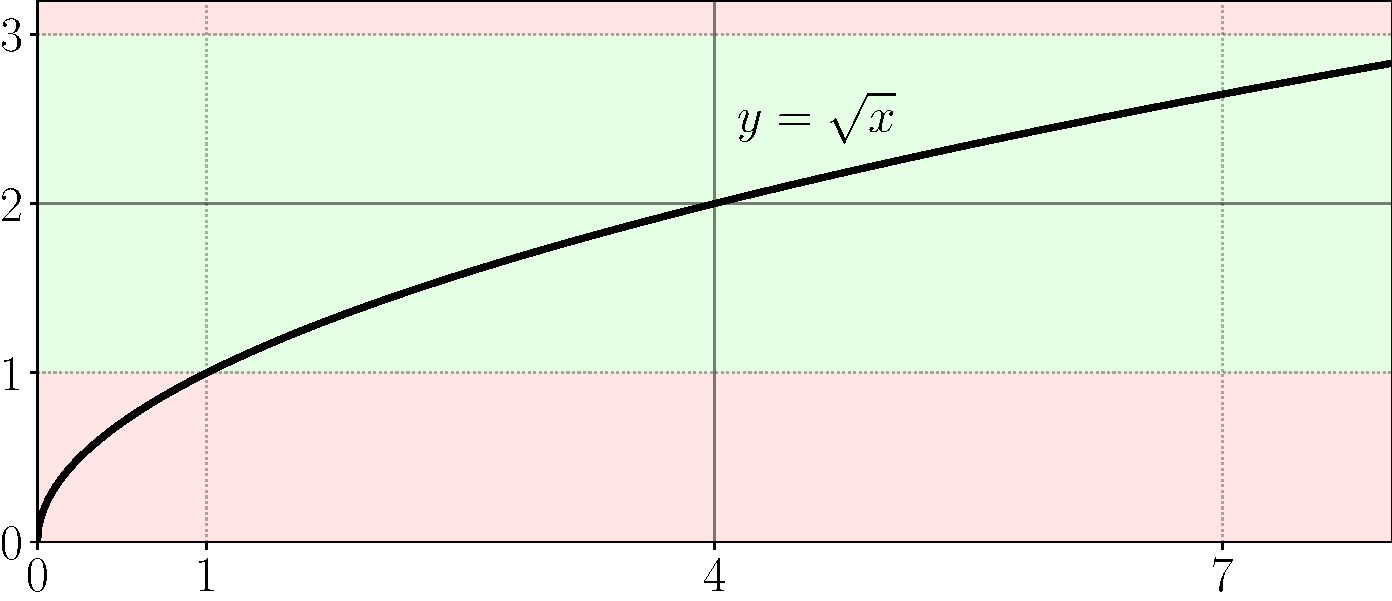
\includegraphics[width=0.9\textwidth]{UA_Figures/UA_ex4_2_2_fig_1.pdf}
        \end{center}

        \item Since \( [[x]] \) is always an integer, we have \( \abs{[[x]] - 3} < 1 \) if and only if \( [[x]] = 3 \), which is the case if and only if \( 3 \leq x < 4 \). So we should choose the largest possible \( \delta \) such that \( V_{\delta}(\pi) \subseteq [3, 4) \), which is
        \[
            \delta = \min \{ \pi - 3, 4 - \pi \} = \pi - 3.
        \]
        \begin{center}
            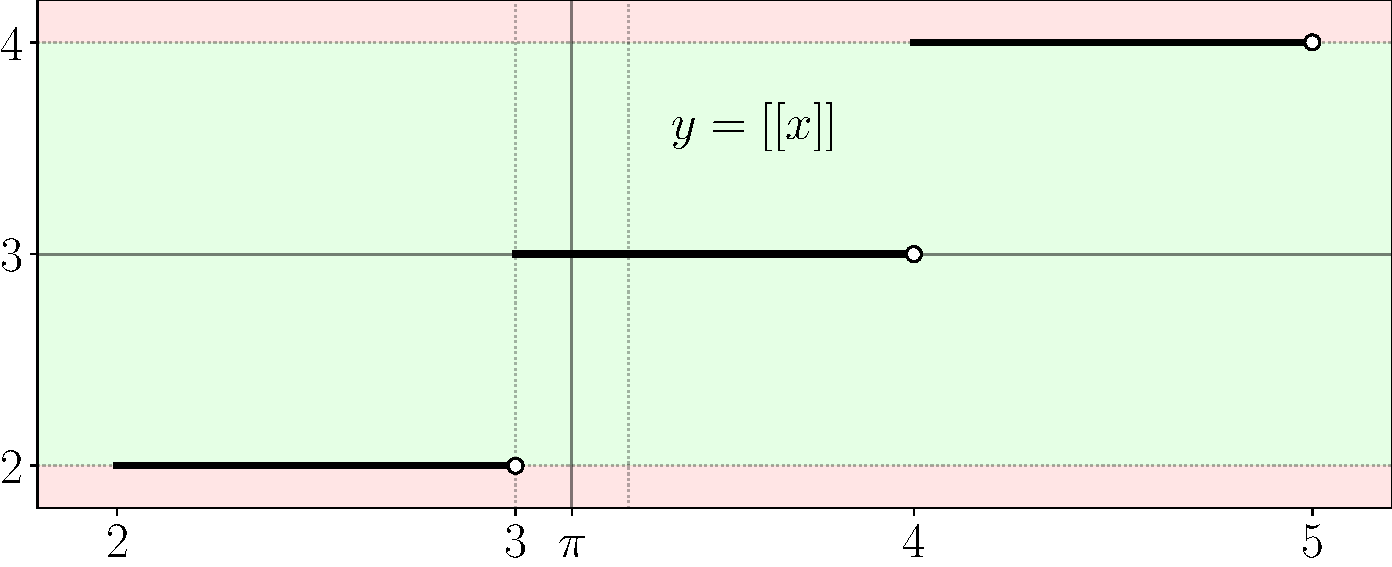
\includegraphics[width=0.9\textwidth]{UA_Figures/UA_ex4_2_2_fig_2.pdf}
        \end{center}

        \item As in part (c), we have \( \abs{[[x]] - 3} < 0.01 \) if and only if \( [[x]] = 3 \), so the largest possible choice is \( \delta = \pi - 3 \). (The following graph is not to scale.)
        \begin{center}
            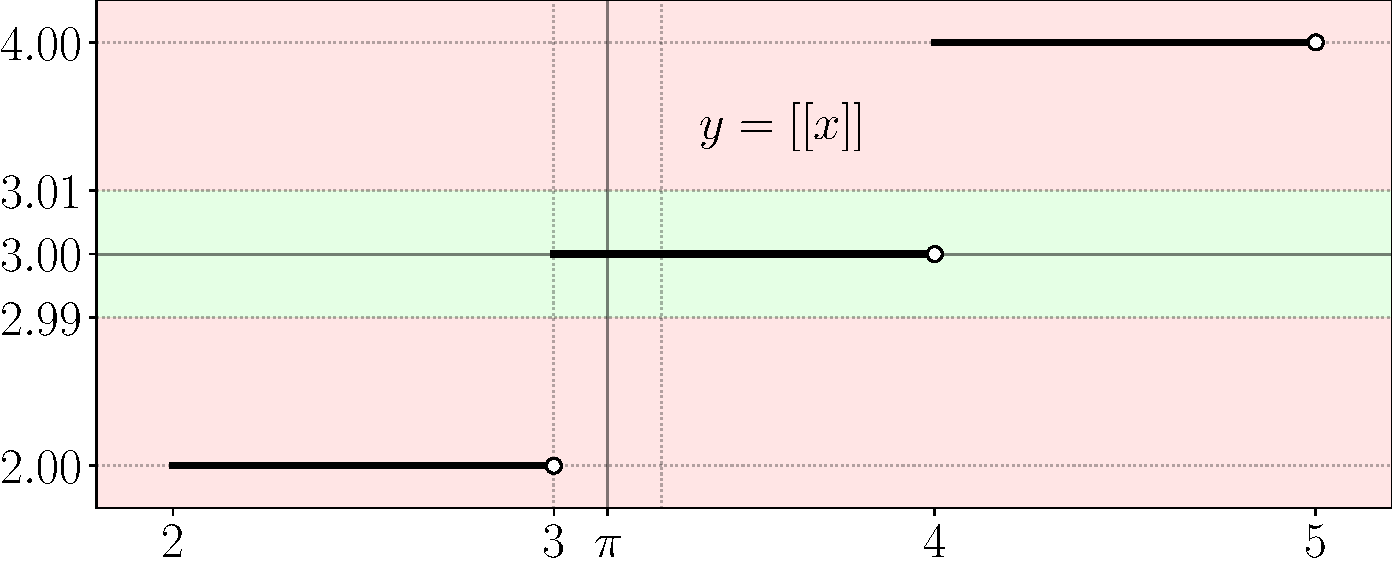
\includegraphics[width=0.9\textwidth]{UA_Figures/UA_ex4_2_2_fig_3.pdf}
        \end{center}
    \end{enumerate}
\end{solution}

\begin{exercise}
\label{ex:4.2.3}
    Review the definition of Thomae's function \( t(x) \) from Section 4.1.
    \begin{enumerate}
        \item Construct three different sequences \( (x_n), (y_n), \) and \( (z_n) \), each of which converges to 1 without using the number 1 as a term in the sequence.

        \item Now, compute \( \lim t(x_n), \lim t(y_n), \) and \( \lim t(z_n) \).

        \item Make an educated conjecture for \( \lim_{x \to 1} t(x) \), and use Definition 4.2.1B to verify the claim. (Given \( \epsilon > 0 \), consider the set of points \( \{ x \in \R : t(x) \geq \epsilon \} \). Argue that all the points in this set are isolated.)
    \end{enumerate}
\end{exercise}

\begin{solution}
    \begin{enumerate}
        \item Take
        \[
            x_n = 1 + \frac{1}{n}, \quad y_n = 1 - \frac{1}{n}, \hspaceand z_n = 1 + \frac{\sqrt{2}}{n}.
        \]

        \item Since \( x_n = \tfrac{n+1}{n} \), we have \( t(x_n) = \tfrac{1}{n} \) and thus \( \lim t(x_n) = 0 \). Similarly, \( y_n = \tfrac{n-1}{n} \), so \( t(y_1) = t(0) = 1 \) and \( t(y_n) = \tfrac{1}{n} \) for \( n \geq 2 \), so that \( \lim t(y_n) = 0 \) also. Finally, since \( z_n \in \I \) for each \( n \in \N \), we have \( \lim t(z_n) = 0 \).

        \item We conjecture that \( \lim_{x \to 1} t(x) = 0 \). To see this, first let us prove the following lemma.

        \begin{lemma}
        \label{lem:ex4.2.3}
            Suppose \( x \in \R \) and \( n \in \N \). There exists a \( \delta > 0 \) such that if \( \tfrac{a}{b} \neq x \) is a rational number contained in \( V_{\delta}(x) \) with \( b > 0 \), then \( b > n \).

        \end{lemma}
        \begin{proof}
            Suppose \( b \in \N \) is such that \( 1 \leq b \leq n \). Since \( I := \bkt{ x - 1, x + 1 } \) is an interval of length 2, there are either \( 2b \) or \( 2b + 1 \) rationals of the form \( \tfrac{a}{b} \) contained in \( I \). (To fit the most rationals inside \( I \), we should place the first such rational \( \tfrac{a}{b} \) on the left endpoint \( x - 1 \); then \( \tfrac{a + 2b}{b} = \tfrac{a}{b} + 2 = x + 1 \) is the right endpoint. Thus we have the \( 2b + 1 \) rational numbers \( \tfrac{a}{b}, \tfrac{a + 1}{b}, \ldots, \tfrac{a + 2b}{b} \) contained in \( I \). In the general case, the left endpoint will not be of the form \( \tfrac{a}{b} \) and so there will be only \( 2b \) rationals of this form contained in \( I \).) Given this, the set
            \[
                A = \set{ \abs{x - \frac{a}{b}} : \frac{a}{b} \in I, \frac{a}{b} \neq x, 1 \leq b \leq n }
            \]
            is non-empty and finite, so that \( \delta := \min A \) exists (\Cref{lem:ex1.3.2}); notice that \( \delta > 0 \) since each element of \( A \) is strictly positive. It follows that \( V_{\delta}(x) \) can contain only rationals \( \tfrac{a}{b} \) with denominators \( b > n \), other than possibly \( x \) itself.
        \end{proof}

        Now we can prove that \( \lim_{x \to 1} t(x) = 0 \). Let \( \epsilon > 0 \) be given and let \( n \in \N \) be such that \( \tfrac{1}{n} < \epsilon \). By \Cref{lem:ex4.2.3}, there exists a \( \delta > 0 \) such that if \( \tfrac{a}{b} \neq 1 \) is a rational number contained in \( V_{\delta}(1) \), then \( b > n \). Suppose \( x \in V_{\delta}(1) \). If \( x \) is irrational then \( t(x) = 0 \in V_{\epsilon}(0) \), and if \( x = \tfrac{a}{b} \neq 1 \) is rational then
        \[
            0 \leq t(x) = \frac{1}{b} < \frac{1}{n} < \epsilon \implies t(x) \in V_{\epsilon}(0).
        \]
        In either case, \( x \in V_{\delta}(1) \setminus \{ 1 \} \) implies that \( t(x) \in V_{\epsilon}(0) \) and thus \( \lim_{x \to 1} t(x) = 0 \).
    \end{enumerate}
\end{solution}

\begin{exercise}
\label{ex:4.2.4}
    Consider the reasonable but erroneous claim that
    \[
        \lim_{x \to 10} 1/[[x]] = 1/10.
    \]
    \begin{enumerate}
        \item Find the largest \( \delta \) that represents a proper response to the challenge of \( \epsilon = 1/2 \).

        \item Find the largest \( \delta \) that represents a proper response to \( \epsilon = 1/50 \).

        \item Find the largest \( \epsilon \) challenge for which there is no suitable \( \delta \) response possible.
    \end{enumerate}
\end{exercise}

\begin{solution}
    Let \( f(x) = \tfrac{1}{[[x]]} \), which is defined provided \( [[x]] \neq 0 \), which is the case if and only if \( x < 0 \) or \( x \geq 1 \). Thus the domain of \( f \) is \( A = (-\infty, 0) \cup [1, \infty) \).
    \begin{enumerate}
        \item Let \( \delta = 8 \) and observe that
        \[
            x \in V_{\delta}(10) = (2, 18) \implies f(x) \in \bkt{ \frac{1}{17}, \frac{1}{2} } \subseteq \paren{ -\frac{2}{5}, \frac{3}{5} } = V_{1/2}\paren{ \frac{1}{10} }.
        \]
        Thus \( \delta = 8 \) is a valid response to the challenge of \( \epsilon = \tfrac{1}{2} \). If \( \delta > 8 \), then there exists an \( x \in V_{\delta}(10) \) such that \( 1 \leq x < 2 \), which gives \( f(x) = 1 \not\in \paren{ -\tfrac{2}{5}, \tfrac{3}{5} } = V_{1/2} \paren{ \tfrac{1}{10} } \). Hence \( \delta = 8 \) is the largest proper response to the challenge of \( \epsilon = \tfrac{1}{2} \).
        \begin{center}
            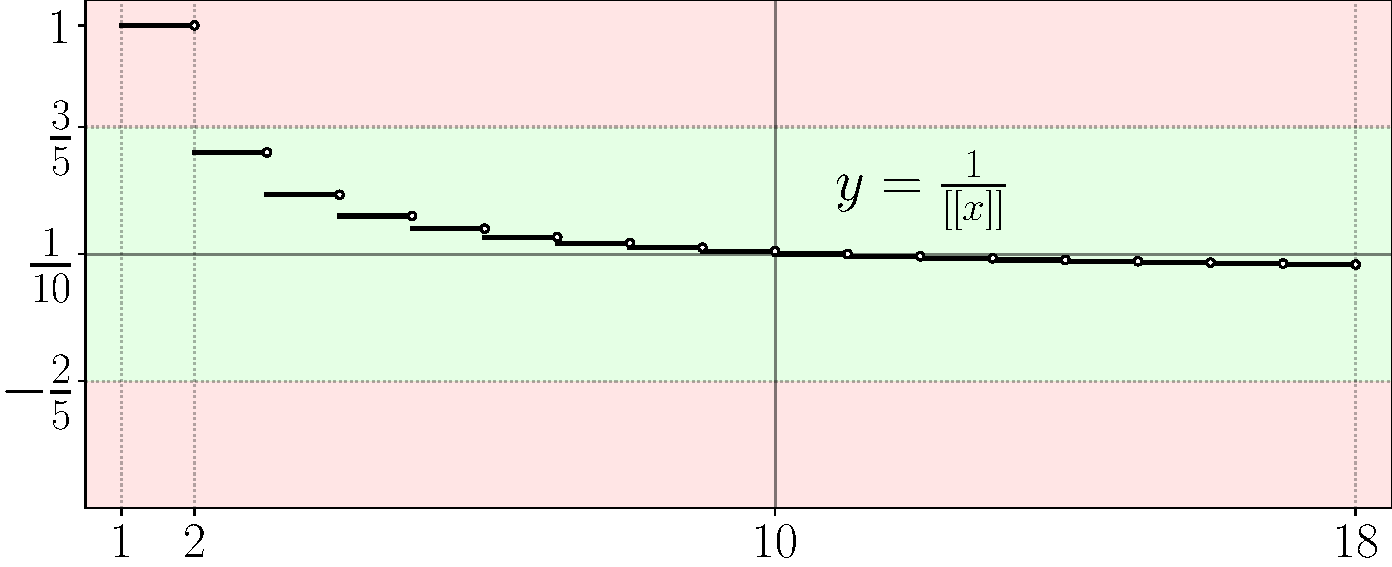
\includegraphics[width=0.9\textwidth]{UA_Figures/UA_ex4_2_4_fig_1.pdf}
        \end{center}

        \item Let \( \delta = 1 \) and observe that
        \[
            x \in V_{\delta}(10) = (9, 11) \implies f(x) \in \bkt{ \frac{1}{10}, \frac{1}{9} } \subseteq \paren{ \frac{2}{25}, \frac{3}{25} } = V_{1/50} \paren{ \frac{1}{10} }.
        \]
        Thus \( \delta = 1 \) is a valid response to the challenge of \( \epsilon = \tfrac{1}{50} \). If \( \delta > 1 \), then there exists an \( x \in V_{\delta}(10) \) such that \( 8 \leq x < 9 \), which gives \( f(x) = \tfrac{1}{8} \not\in \paren{ \tfrac{2}{25}, \tfrac{3}{25} } = V_{1/50} \paren{ \tfrac{1}{10} } \). Hence \( \delta = 1 \) is the largest proper response to the challenge of \( \epsilon = \tfrac{1}{50} \).
        \begin{center}
            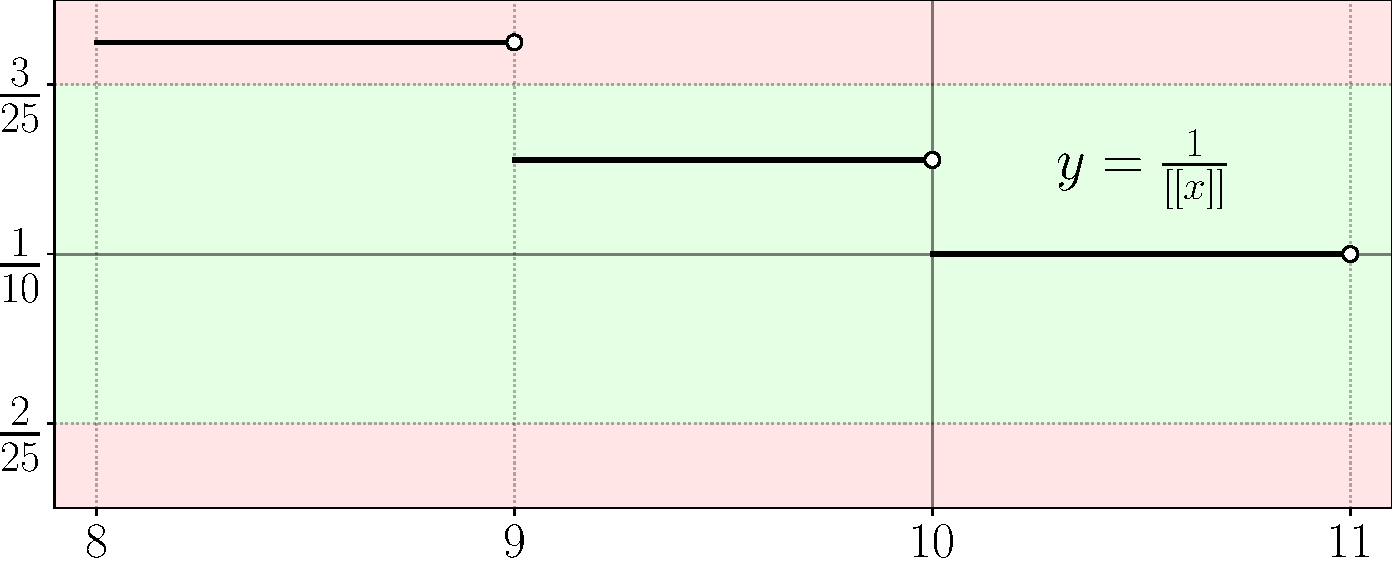
\includegraphics[width=0.9\textwidth]{UA_Figures/UA_ex4_2_4_fig_2.pdf}
        \end{center}

        \item Suppose that \( \epsilon = \tfrac{1}{90} \) and \( \delta > 0 \). Notice that there exists an \( x \in V_{\delta}(10) \) such that \( 9 \leq x < 10 \), which gives \( f(x) = \tfrac{1}{9} \not\in \paren{ \tfrac{4}{45}, \tfrac{1}{9} } = V_{\epsilon} \paren{ \tfrac{1}{10} } \). Thus there is no valid \( \delta \) response to the challenge of \( \epsilon = \tfrac{1}{90} \).
        
        Now suppose \( \epsilon > \tfrac{1}{90} \), let \( \delta = 1 \), and observe that
        \[
            x \in V_{\delta}(10) = (9, 11) \implies f(x) \in \bkt{ \frac{1}{10}, \frac{1}{9} } \subseteq V_{\epsilon} \paren{ \frac{1}{10} }.
        \]
        Thus \( \delta = 1 \) is a valid response to this \( \epsilon \).

        We may conclude that \( \epsilon = \tfrac{1}{90} \) is the largest challenge for which there is no suitable \( \delta \) response possible.
        \begin{center}
            \includegraphics[width=0.9\textwidth]{UA_Figures/UA_ex4_2_4_fig_3.pdf}
        \end{center}
    \end{enumerate}
\end{solution}

\begin{exercise}
\label{ex:4.2.5}
    Use Definition 4.2.1 to supply a proper proof for the following limit statements.
    \begin{enumerate}
        \item \( \lim_{x \to 2} (3x + 4) = 10 \).

        \item \( \lim_{x \to 0} x^3 = 0 \).

        \item \( \lim_{x \to 2} (x^2 + x - 1) = 5 \).

        \item \( \lim_{x \to 3} 1/x = 1/3 \).
    \end{enumerate}
\end{exercise}

\begin{solution}
    \begin{enumerate}
        \item Let \( \epsilon > 0 \) be given and let \( \delta = \tfrac{\epsilon}{3} \). If \( x \in \R \) is such that \( 0 < \abs{x - 2} < \delta \), then
        \[
            \abs{(3x + 4) - 10} = \abs{3x - 6} = 3 \abs{x - 2} < 3 \delta = \epsilon.
        \]
        Thus \( \lim_{x \to 2} (3x + 4) = 10 \).

        \item Let \( \epsilon > 0 \) be given and let \( \delta = \epsilon^{1/3} \). If \( x \in \R \) is such that \( 0 < \abs{x} < \delta \), then
        \[
            \abs{x^3} = \abs{x}^3 < \delta^3 = \epsilon.
        \]
        Thus \( \lim_{x \to 0} x^3 = 0 \).

        \item Let \( \epsilon > 0 \) be given. Observe that if \( \abs{x - 2} < 1 \), i.e., \( x \in (1, 3) \), then \( x + 3 \in (4, 7) \). Let \( \delta = \min \set{ \tfrac{\epsilon}{7}, 1 } \). If \( x \in \R \) is such that \( 0 < \abs{x - 2} < \delta \), then
        \[
            \abs{x^2 + x - 1 - 5} = \abs{x + 3} \abs{x - 2} < 7 \delta \leq \epsilon.
        \]
        Thus \( \lim_{x \to 2} (x^2 + x - 1) = 5 \).

        \item Let \( \epsilon > 0 \) be given. Observe that if \( \abs{x - 3} < 1 \), i.e., \( x \in (2, 4) \), then \( \tfrac{1}{3x} \in \paren{ \tfrac{1}{12}, \tfrac{1}{6} } \). Let \( \delta = \min \{ 6 \epsilon, 1 \} \) and note that if \( x \in \R \setminus \{ 0 \} \) is such that \( 0 < \abs{x - 3} < \delta \), then
        \[
            \abs{\frac{1}{x} - \frac{1}{3}} = \frac{\abs{x - 3}}{\abs{3x}} < \frac{\delta}{6} \leq \epsilon.
        \]
        Thus \( \lim_{x \to 3} \tfrac{1}{x} = \tfrac{1}{3} \).
    \end{enumerate}
\end{solution}

\begin{exercise}
\label{ex:4.2.6}
    Decide if the following claims are true or false, and give short justifications of each conclusion.
    \begin{enumerate}
        \item If a particular \( \delta \) has been constructed as a suitable response to a particular \( \epsilon \) challenge, then any smaller positive \( \delta \) will also suffice.

        \item If \( \lim_{x \to a} f(x) = L \) and \( a \) happens to be in the domain of \( f \), then \( L = f(a) \).

        \item If \( \lim_{x \to a} f(x) = L \), then \( \lim_{x \to a} 3[f(x) - 2]^2 = 3(L - 2)^2 \).

        \item If \( \lim_{x \to a} f(x) = 0 \), then \( \lim_{x \to a} f(x) g(x) = 0 \) for any function \( g \) (with domain equal to the domain of \( f \).)
    \end{enumerate}
\end{exercise}

\begin{solution}
    \begin{enumerate}
        \item This is true, since if \( 0 < \delta' < \delta \) then \( V_{\delta'}(c) \subseteq V_{\delta}(c) \) for any \( c \in \R \).

        \item This is false. For a counterexample, consider Thomae's function \( t \). In \Cref{ex:4.2.3} we showed that \( \lim_{x \to 1} t(x) = 0 \), but \( t(1) = 1 \).

        \item This is true and follows from several applications of the Algebraic Limit Theorem for Functional Limits (Corollary 4.2.4).

        \item This is false. Define \( f, g : \R \setminus \{ 0 \} \to \R \) by \( f(x) = x \) and \( g(x) = \tfrac{1}{x} \). It is straightforward to verify that \( \lim_{x \to 0} f(x) = 0 \), but \( \lim_{x \to 0} f(x) g(x) = \lim_{x \to 0} 1 = 1 \).
    \end{enumerate}
\end{solution}

\begin{exercise}
\label{ex:4.2.7}
    Let \( g : A \to \R \) and assume that \( f \) is a bounded function on \( A \) in the sense that there exists \( M > 0 \) satisfying \( \abs{f(x)} \leq M \) for all \( x \in A \).

    Show that if \( \lim_{x \to c} g(x) = 0 \), then \( \lim_{x \to c} g(x) f(x) = 0 \) as well.
\end{exercise}

\begin{solution}
    Let \( \epsilon > 0 \) be given. Since \( \lim_{x \to c} g(x) = 0 \), there is a \( \delta > 0 \) such that \( 0 < \abs{x - c} < \delta \) and \( x \in A \) implies that \( \abs{g(x)} < \tfrac{\epsilon}{M} \). Observe that for such \( x \) we have
    \[
        \abs{f(x) g(x)} = \abs{f(x)} \abs{g(x)} < M \frac{\epsilon}{M} = \epsilon.
    \]
    Thus \( \lim_{x \to c} g(x) f(x) = 0 \).
\end{solution}

\begin{exercise}
\label{ex:4.2.8}
    Compute each limit or state that it does not exist. Use the tools developed in this section to justify each conclusion.
    \begin{enumerate}
        \item \( \lim_{x \to 2} \tfrac{\abs{x-2}}{x-2} \)

        \item \( \lim_{x \to 7/4} \tfrac{\abs{x-2}}{x-2} \)

        \item \( \lim_{x \to 0} (-1)^{[[1/x]]} \)

        \item \( \lim_{x \to 0} \sqrt[3]{x} (-1)^{[[1/x]]} \)
    \end{enumerate}
\end{exercise}

\begin{solution}
    \begin{enumerate}
        \item Let \( f : \R \setminus \{ 2 \} \to \R \) be given by \( f(x) = \tfrac{\abs{x-2}}{x-2} \). Observe that
        \[
            f(x) = \begin{cases}
                1 & \text{if } x > 2, \\
                -1 & \text{if } x < 2.
            \end{cases}
        \]
        We claim that \( \lim_{x \to 2} f(x) \) does not exist. To see this, consider the sequences \( (x_n) \) and \( (y_n) \) given by \( x_n = 2 + \tfrac{1}{n} \) and \( y_n = 2 - \tfrac{1}{n} \), which satisfy \( \lim_{n \to \infty} x_n = \lim_{n \to \infty} y_n = 2 \). However,
        \[
            \lim_{n \to \infty} f(x_n) = \lim_{n \to \infty} 1 = 1 \neq -1 = \lim_{n \to \infty} -1 = \lim_{n \to \infty} f(y_n).
        \]
        Our claim now follows from Corollary 4.2.5.

        \item Define \( f \) as in part (a). We claim that \( \lim_{x \to 7/4} f(x) = -1 \). To see this, let \( \epsilon > 0 \) be given. If \( x \in \R \setminus \{ 2 \} \) is such that \( 0 < \abs{x - \tfrac{7}{4}} < \tfrac{1}{4} \), i.e., \( x \in \paren{ \tfrac{3}{2}, 2 } \), then
        \[
            \abs{f(x) - (-1)} = \abs{-1 + 1} = 0 < \epsilon.
        \]
        Thus \( \lim_{x \to 7/4} f(x) = -1 \).

        \item We claim that \( \lim_{x \to 0} (-1)^{[[1/x]]} \) does not exist. To see this, consider the sequences \( (x_n) \) and \( (y_n) \) given by \( x_n = \tfrac{1}{2n} \) and \( y_n = \tfrac{1}{2n+1} \), which satisfy \( \lim_{n \to \infty} x_n = \lim_{n \to \infty} y_n = 0 \). However,
        \begin{multline*}
            \lim_{n \to \infty} (-1)^{[[1/x_n]]} = \lim_{n \to \infty} (-1)^{[[2n]]} = \lim_{n \to \infty} 1 = 1 \\[2mm]
            \neq -1 = \lim_{n \to \infty} -1 = \lim_{n \to \infty} (-1)^{[[2n+1]]} = \lim_{n \to \infty} (-1)^{[[1/y_n]]}.
        \end{multline*}
        Our claim now follows from Corollary 4.2.5.

        \item Let \( \epsilon > 0 \) be given and let \( \delta = \epsilon^3 \). If \( x \in \R \) is such that \( 0 < \abs{x} < \delta \), then
        \[
            \abs{\sqrt[3]{x}} = \sqrt[3]{\abs{x}} < \sqrt[3]{\delta} = \epsilon.
        \]
        Thus \( \lim_{x \to 0} \sqrt[3]{x} = 0 \). Since the function \( (-1)^{[[1/x]]} \) is evidently bounded, we may apply \Cref{ex:4.2.7} to conclude that \( \lim_{x \to 0} \sqrt[3]{x} (-1)^{[[1/x]]} = 0 \).
    \end{enumerate}
\end{solution}

\begin{exercise}[Infinite Limits]
\label{ex:4.2.9}
    The statement \( \lim_{x \to 0} 1/x^2 = \infty \) certainly makes intuitive sense. To construct a rigorous definition in the challenge-response style of Definition 4.2.1 for an infinite limit statement of this form, we replace the (arbitrarily small) \( \epsilon > 0 \) challenge with an (arbitrarily large) \( M > 0 \) challenge:

    \textit{Definition}: \( \lim_{x \to c} f(x) = \infty \) means that for all \( M > 0 \) we can find a \( \delta > 0 \) such that whenever \( 0 < \abs{x - c} < \delta \), it follows that \( f(x) > M \).
    \begin{enumerate}
        \item Show \( \lim_{x \to 0} 1/x^2 = \infty \) in the sense described in the previous definition.

        \item Now, construct a definition for the statement \( \lim_{x \to \infty} f(x) = L \). Show \( \lim_{x \to \infty} 1/x = 0 \).

        \item What would a rigorous definition for \( \lim_{x \to \infty} f(x) = \infty \) look like? Give an example of such a limit.
    \end{enumerate}
\end{exercise}

\begin{solution}
    \begin{enumerate}
        \item Let \( M > 0 \) be given and let \( \delta = \tfrac{1}{\sqrt{M}} > 0 \). If \( x \in \R \) is such that \( 0 < \abs{x} < \delta \), then observe that
        \[
            \frac{1}{\abs{x}} > \sqrt{M} > 0 \implies \frac{1}{x^2} > M.
        \]
        It follows that \( \lim_{x \to 0} \tfrac{1}{x^2} = \infty \).

        \item The statement \( \lim_{x \to \infty} f(x) = L \) means that for all \( \epsilon > 0 \) we can find an \( M > 0 \) such that whenever \( x > M \), it follows that \( \abs{f(x) - L} < \epsilon \).

        To see that \( \lim_{x \to \infty} \tfrac{1}{x} = 0 \), let \( \epsilon > 0 \) be given, let \( M = \tfrac{1}{\epsilon} \), and observe that
        \[
            x > M = \frac{1}{\epsilon} \implies \frac{1}{x} < \epsilon.
        \]

        \item The statement \( \lim_{x \to \infty} f(x) = \infty \) means that for all \( M > 0 \) we can find a \( K > 0 \) such that whenever \( x > K \), it follows that \( f(x) > M \); it is straightforward to verify that \( \lim_{x \to \infty} x = \infty \), for example.
    \end{enumerate}
\end{solution}

\begin{exercise}[Right and Left Limits]
\label{ex:4.2.10}
    Introductory calculus courses typically refer to the \textit{right-hand limit} of a function as the limit obtained by ``letting \( x \) approach \( a \) from the right-hand side.''
    \begin{enumerate}
        \item Give a proper definition in the style of Definition 4.2.1 for the right-hand and left-hand limit statements:
        \[
            \lim_{x \to a^+} f(x) = L \hspaceand \lim_{x \to a^-} f(x) = M.
        \]

        \item Prove that \( \lim_{x \to a} f(x) = L \) if and only if both the right and left-hand limits equal \( L \).
    \end{enumerate}
\end{exercise}

\begin{solution}
    \begin{enumerate}
        \item Suppose we have a function \( f : A \to \R \) and \( a \in \R \) is a limit point of \( A \cap (a, \infty) \). We say that \( \lim_{x \to a^+} f(x) = L \) provided that, for all \( \epsilon > 0 \), there exists a \( \delta > 0 \) such that whenever \( a < x < a + \delta \) and \( x \in A \), it follows that \( \abs{f(x) - L} < \epsilon \). Similarly, if \( a \in \R \) is a limit point of \( A \cap (-\infty, a) \), we say that \( \lim_{x \to a^-} f(x) = M \) provided that, for all \( \epsilon > 0 \), there exists a \( \delta > 0 \) such that whenever \( a - \delta < x < a \) and \( x \in A \), it follows that \( \abs{f(x) - M} < \epsilon \).

        \item If \( \lim_{x \to a} f(x) = L \), then certainly \( \lim_{x \to a^+} f(x) = \lim_{x \to a^-} f(x) = L \), since both of the statements \( a < x < a + \delta \) and \( a - \delta < x < a \) imply that \( 0 < \abs{x - a} < \delta \). Suppose therefore that \( \lim_{x \to a^+} f(x) = \lim_{x \to a^-} f(x) = L \) and let \( \epsilon > 0 \) be given. There are positive real numbers \( \delta_1 \) and \( \delta_2 \) such that
        \[
            a < x < a + \delta_1 \implies \abs{f(x) - L} < \epsilon \hspaceand a - \delta_2 < x < a \implies \abs{f(x) - L} < \epsilon.
        \]
        Let \( \delta = \min \{ \delta_1, \delta_2 \} \). If \( x \in \R \) is such that \( 0 < \abs{x - a} < \delta \), then either
        \begin{gather*}
            a < x < a + \delta < a + \delta_1 \implies \abs{f(x) - L} < \epsilon, \text{ or} \\[2mm]
            a - \delta_2 < a - \delta < x < a \implies \abs{f(x) - L} < \epsilon.
        \end{gather*}
        In either case we have \( \abs{f(x) - L} < \epsilon \) and hence \( \lim_{x \to a} f(x) = L \).
    \end{enumerate}
\end{solution}

\begin{exercise}[Squeeze Theorem]
\label{ex:4.2.11}
    Let \( f, g, \) and \( h \) satisfy \( f(x) \leq g(x) \leq h(x) \) for all \( x \) in some common domain \( A \). If \( \lim_{x \to c} f(x) = L \) and \( \lim_{x \to c} h(x) = L \) at some limit point \( c \) of \( A \), show \( \lim_{x \to c} g(x) = L \).
\end{exercise}

\begin{solution}
    Suppose \( (x_n) \) is a sequence contained in \( A \) satisfying \( x_n \neq c \) and \( \lim_{n \to \infty} x_n = c \). By assumption, we have \( f(x_n) \leq g(x_n) \leq h(x_n) \) for all \( n \in \N \), and Theorem 4.2.3 guarantees that \( \lim_{n \to \infty} f(x_n) = \lim_{n \to \infty} h(x_n) = L \). We may now apply the Squeeze Theorem for sequences (\Cref{ex:2.3.3}) to see that \( \lim_{n \to \infty} g(x_n) = L \), and Theorem 4.2.3 then allows us to conclude that \( \lim_{x \to c} g(x) = L \).
\end{solution}

\section{Continuous Functions}
\label{sec:4.3}

\begin{exercise}
\label{ex:4.3.1}
    Let \( g(x) = \sqrt[3]{x} \).
    \begin{enumerate}
        \item Prove that \( g \) is continuous at \( c = 0 \).

        \item Prove that \( g \) is continuous at a point \( c \neq 0 \). (The identity \( a^3 - b^3 = (a - b)(a^2 + ab + b^2) \) will be helpful.)
    \end{enumerate}
\end{exercise}

\begin{solution}
    \begin{enumerate}
        \item Let \( \epsilon > 0 \) be given and let \( \delta = \epsilon^3 \). If we take \( x \in \R \) such that \( \abs{x} < \delta \), then we will have
        \[
            \abs{\sqrt[3]{x}} = \sqrt[3]{\abs{x}} < \sqrt[3]{\delta} = \epsilon.
        \]
        Thus \( g \) is continuous at \( c = 0 \).

        \item Taking \( a = x^{1/3} \) and \( b = c^{1/3} \) in the identity \( a^3 - b^3 = (a - b)(a^2 + ab + b^2) \) gives
        \begin{align*}
            x - c &= \paren{ x^{1/3} - c^{1/3} } \paren{ x^{2/3} + (xc)^{1/3} + c^{2/3} } \\[2mm]
            \implies \abs{x - c} &= \abs{x^{1/3} - c^{1/3}} \abs{x^{2/3} + (xc)^{1/3} + c^{2/3}}.
        \end{align*}
        If we take \( x \) close enough to \( c \) so that \( x \) and \( c \) have the same sign, i.e., take \( x \) such that \( \abs{x - c} < \abs{c} \), then \( xc > 0 \) and so
        \[
            \abs{x^{2/3} + (xc)^{1/3} + c^{2/3}} = x^{2/3} + (xc)^{1/3} + c^{2/3} \geq c^{2/3}.
        \]
        Let \( \delta = \min \{ \abs{c}, c^{2/3} \epsilon \} \) and suppose \( x \in \R \) is such that \( \abs{x - c} < \delta \). By the previous discussion, we then have
        \[
            \abs{x^{1/3} - c^{1/3}} \leq \frac{\abs{x - c}}{c^{2/3}} < \frac{\delta}{c^{2/3}} < \epsilon.
        \]
        Thus \( g \) is continuous at \( c \).
    \end{enumerate}
\end{solution}

\begin{exercise}
\label{ex:4.3.2}
    To gain a deeper understanding of the relationship between \( \epsilon \) and \( \delta \) in the definition of continuity, let's explore some modest variations of Definition 4.3.1. In all of these, let \( f \) be a function defined on all of \( \R \).
    \begin{enumerate}
        \item Let's say \( f \) is \textit{onetinuous} at \( c \) if for all \( \epsilon > 0 \) we can choose \( \delta = 1 \) and it follows that \( \abs{f(x) - f(c)} < \epsilon \) whenever \( \abs{x - c} < \delta \). Find an example of a function that is onetinuous on all of \( \R \).

        \item Let's say \( f \) is \textit{equaltinuous} at \( c \) if for all \( \epsilon > 0 \) we can choose \( \delta = \epsilon \) and it follows that \( \abs{f(x) - f(c)} < \epsilon \) whenever \( \abs{x - c} < \delta \). Find an example of a function that is equaltinuous on \( \R \) that is nowhere onetinuous, or explain why there is no such function.
        
        \item Let's say \( f \) is \textit{lesstinuous} at \( c \) if for all \( \epsilon > 0 \) we can choose \( 0 < \delta < \epsilon \) and it follows that \( \abs{f(x) - f(c)} < \epsilon \) whenever \( \abs{x - c} < \delta \). Find an example of a function that is lesstinuous on \( \R \) that is nowhere equaltinuous, or explain why there is no such function.

        \item Is every lesstinuous function continuous? Is every continuous function lesstinuous? Explain.
    \end{enumerate}
\end{exercise}

\begin{solution}
    \begin{enumerate}
        \item Let \( f \) be given by \( f(x) = 0 \) for all \( x \in \R \). Fix \( c \in \R \) and let \( \epsilon > 0 \) be given. If \( x \in \R \) is such that \( \abs{x - c} < 1 \), then
        \[
            \abs{f(x) - f(c)} = \abs{0 - 0} = 0 < \epsilon.
        \]
        Thus \( f \) is onetinuous on \( \R \).

        \item Let \( f \) be given by \( f(x) = x \) for all \( x \in \R \). Fix \( c \in \R \) and let \( \epsilon > 0 \) be given. If \( x \in \R \) is such that \( \abs{x - c} < \epsilon \), then
        \[
            \abs{f(x) - f(c)} = \abs{x - c} < \epsilon.
        \]
        Thus \( f \) is equaltinuous on \( \R \). However, \( f \) is nowhere onetinuous. Fix \( c \in \R \) again and consider \( \epsilon = \tfrac{1}{4} \). Note that \( x = c + \tfrac{1}{2} \) satisfies \( \abs{x - c} = \abs{c + \tfrac{1}{2} - c} = \tfrac{1}{2} < 1 \), however
        \[
            \abs{f(x) - f(c)} = \abs{x - c} = \frac{1}{2} > \frac{1}{4} = \epsilon.
        \]
        Thus \( f \) is nowhere onetinuous.

        \item Let \( f \) be given by \( f(x) = 2x \) for all \( x \in \R \). Fix \( c \in \R \), let \( \epsilon > 0 \) be given, and let \( \delta = \tfrac{\epsilon}{2} < \epsilon \). If \( x \in \R \) is such that \( \abs{x - c} < \delta \), then
        \[
            \abs{f(x) - f(c)} = 2 \abs{x - c} < 2 \delta = \epsilon.
        \]
        Thus \( f \) is lesstinuous on \( \R \). However, \( f \) is nowhere equaltinuous. Fix \( c \in \R \) again and let \( \epsilon = 1 \). Note that \( x = c + \tfrac{3}{4} \) satisfies \( \abs{x - c} = \tfrac{3}{4} < \epsilon \), however
        \[
            \abs{f(x) - f(c)} = 2 \abs{x - c} = \frac{3}{2} > \epsilon.
        \]
        Thus \( f \) is nowhere equaltinuous.

        \item It is clear that every lesstinuous function is continuous. We claim that every continuous function is lesstinuous. To see this, let \( f \) be a continuous function. Fix \( c \in \R \) and \( \epsilon > 0 \). Since \( f \) is continuous at \( c \), there is a \( \delta' > 0 \) such that \( \abs{f(x) - f(c)} < \epsilon \) whenever \( \abs{x - c} < \delta' \). Let \( \delta = \min \{ \delta', \tfrac{\epsilon}{2} \} \), so that \( 0 < \delta < \epsilon \), and observe that if \( x \in \R \) is such that \( \abs{x - c} < \delta \) then \( x \) also satisfies \( \abs{x - c} < \delta' \), whence \( \abs{f(x) - f(c)} < \epsilon \).
    \end{enumerate}
\end{solution}

\begin{exercise}
\label{ex:4.3.3}
    \begin{enumerate}
        \item Supply a proof for Theorem 4.3.9 using the \( \epsilon \)-\( \delta \) characterization of continuity.

        \item Give another proof of this theorem using the sequential characterization of continuity (from Theorem 4.3.2 (iii)).
    \end{enumerate}
\end{exercise}

\begin{solution}
    \begin{enumerate}
        \item Let \( a \in A \) and \( \epsilon > 0 \) be given. By assumption we have \( f(a) \in B \), so \( g \) is continuous at \( f(a) \). There then exists a \( \delta_1 > 0 \) such that
        \begin{equation}
            \abs{y - f(a)} < \delta_1 \text{ and } y \in B \implies \abs{g(y) - g(f(a))} < \epsilon.
        \end{equation}
        Since \( f \) is continuous at \( a \), there exists a \( \delta_2 > 0 \) such that
        \begin{equation}
            \abs{x - a} < \delta_2 \text{ and } x \in A \implies \abs{f(x) - f(a)} < \delta_1.
        \end{equation}
        Combining (1) and (2), we have
        \begin{multline*}
            \abs{x - a} < \delta_2 \text{ and } x \in A \implies \abs{f(x) - f(a)} < \delta_1 \text{ and } f(x) \in B \\ \implies \abs{g(f(x)) - g(f(a))} < \epsilon.
        \end{multline*}
        Thus \( g \circ f \) is continuous at \( a \).

        \item Let \( a \in A \) be given and suppose \( (a_n)_{n=1}^{\infty} \) is contained in \( A \) and satisfies \( \lim_{n \to \infty} a_n = a \). Since \( f \) is continuous at \( a \), Theorem 4.3.2 (iii) gives us \( \lim_{n \to \infty} f(a_n) = f(a) \). By assumption \( g \) is continuous at \( f(a) \in B \) and \( (f(a_n))_{n=1}^{\infty} \) is contained in \( B \), so Theorem 4.3.2 (iii) gives us \( \lim_{n \to \infty} g(f(a_n)) = g(f(a)) \). One more application of Theorem 4.3.2 (iii) allows us to conclude that \( g \circ f \) is continuous at \( a \).
    \end{enumerate}
\end{solution}

\begin{exercise}
\label{ex:4.3.4}
    Assume \( f \) and \( g \) are defined on all of \( \R \) and that \( \lim_{x \to p} f(x) = q \) and \( \lim_{x \to q} g(x) = r \).
    \begin{enumerate}
        \item Give an example to show that it may not be true that
        \[
            \lim_{x \to p} g(f(x)) = r.
        \]

        \item Show that the result in (a) does follow if we assume \( f \) and \( g \) are continuous.

        \item Does the result in (a) hold if we only assume \( f \) is continuous? How about if we only assume that \( g \) is continuous?
    \end{enumerate}
\end{exercise}

\begin{solution}
    \begin{enumerate}
        \item Let \( f \) be given by \( f(x) = 0 \) for all \( x \in \R \) and let \( g \) be given by
        \[
            g(x) = \begin{cases}
                0 & \text{if } x \neq 0, \\
                1 & \text{if } x = 0.
            \end{cases}
        \]
        We have \( \lim_{x \to 0} f(x) = \lim_{x \to 0} g(x) = 0 \), however note that \( g(f(x)) = g(0) = 1 \) for all \( x \in \R \). It follows that
        \[
            \lim_{x \to 0} g(f(x)) = 1 \neq 0.
        \]

        \item By Theorem 4.3.9, the composition \( g \circ f \) is continuous. Since \( f \) and \( g \) are defined on all of \( \R \), Theorem 4.3.2 (iv) lets us write
        \[
            \lim_{x \to p} g(f(x)) = g(f(p)) = g \paren{ \lim_{x \to p} f(x) } = g(q) = \lim_{x \to q} g(x).
        \]

        \item As the counterexample in part (a) shows, the result does not hold if we only assume that \( f \) is continuous. However, it does hold if we assume that \( g \) is continuous. To see this, let \( (x_n) \) be some sequence satisfying \( \lim_{n \to \infty} x_n = p \) and \( x_n \neq p \). Theorem 4.2.3 shows that \( \lim f(x_n) = q \), and since \( g \) is continuous the sequential characterization of continuity (Theorem 4.3.2 (iii)) implies that
        \[
            \lim g(f(x_n)) = g(q) = r,
        \]
        where the last equality also follows from the continuity of \( g \). Theorem 4.2.3 allows us to conclude that
        \[
            \lim_{x \to p} g(f(x)) = r.
        \]
    \end{enumerate}
\end{solution}

\begin{exercise}
\label{ex:4.3.5}
    Show using Definition 4.3.1 that if \( c \) is an isolated point of \( A \subseteq \R \), then \( f : A \to \R \) is continuous at \( c \).
\end{exercise}

\begin{solution}
    Since \( c \) is an isolated point of \( A \), there exists a \( \delta > 0 \) such that \( (c - \delta, c + \delta) \cap A = \{ c \} \). Let \( \epsilon > 0 \) be given. If \( x \in A \) is such that \( \abs{x - c} < \delta \), then it must be the case that \( x = c \), which gives us
    \[
        \abs{f(x) - f(c)} = \abs{f(c) - f(c)} = 0 < \epsilon.
    \]
    Thus \( f \) is continuous at \( c \).
\end{solution}

\begin{exercise}
\label{ex:4.3.6}
    Provide an example of each or explain why the request is impossible.
    \begin{enumerate}
        \item Two functions \( f \) and \( g \), neither of which is continuous at 0 such that \( f(x)g(x) \) and \( f(x) + g(x) \) are continuous at 0.

        \item A function \( f(x) \) continuous at 0 and \( g(x) \) not continuous at 0 such that \( f(x) + g(x) \) is continuous at 0.

        \item A function \( f(x) \) continuous at 0 and \( g(x) \) not continuous at 0 such that \( f(x)g(x) \) is continuous at 0.

        \item A function \( f(x) \) not continuous at 0 such that \( f(x) + \tfrac{1}{f(x)} \) is continuous at 0.

        \item A function \( f(x) \) not continuous at 0 such that \( [f(x)]^3 \) is continuous at 0.
    \end{enumerate}
\end{exercise}

\begin{solution}
    \begin{enumerate}
        \item Let \( f, g : \R \to \R \) be given by
        \[
            f(x) = \begin{cases}
                0 & \text{if } x \neq 0, \\
                1 & \text{if } x = 0,
            \end{cases}
            \quad\quad\quad
            g(x) = \begin{cases}
                1 & \text{if } x \neq 0, \\
                0 & \text{if } x = 0.
            \end{cases}
        \]
        Neither \( f \) nor \( g \) is continuous at 0, however note that for all \( x \in \R \) we have
        \[
            f(x)g(x) = 0 \hspaceand f(x) + g(x) = 1.
        \]
        Thus \( fg \) and \( f + g \) are continuous at 0.

        \item This is impossible. If \( f \) and \( f + g \) are continuous at 0 then Theorem 4.3.4 implies that \( g = f + g - f \) is continuous at 0.

        \item If we take \( g \) as in part (a) and let \( f(x) = 0 \) for all \( x \in \R \), then \( g \) is not continuous at 0 but \( f = fg \) is continuous at 0.

        \item Let \( f : \R \to \R \) be given by
        \[
            f(x) = \begin{cases}
                \sqrt{2} - 1 & \text{if } x \neq 0, \\
                \sqrt{2} + 1 & \text{if } x = 0,
            \end{cases}
        \]
        and note that \( f \) is discontinuous at 0. Note further that \( f(x) + \tfrac{1}{f(x)} = 2 \sqrt{2} \) for all \( x \in \R \); it follows that \( f + \tfrac{1}{f} \) is continuous at 0.

        \item This is impossible. As we showed in \Cref{ex:4.3.1}, the function \( g(x) = \sqrt[3]{x} \) is continuous everywhere. Thus if \( [f(x)]^3 \) is continuous at 0, then by Theorem 4.3.9 the composition
        \[
            f(x) = \sqrt[3]{[f(x)]^3}
        \]
        must also be continuous at 0.
    \end{enumerate}
\end{solution}

\begin{exercise}
\label{ex:4.3.7}
    \begin{enumerate}
        \item Referring to the proper theorems, give a formal argument that Dirichlet's function from Section 4.1 is nowhere-continuous on \( \R \).

        \item Review the definition of Thomae's function in Section 4.1 and demonstrate that it fails to be continuous at every rational point.

        \item Use the characterization of continuity in Theorem 4.3.2 (iii) to show that Thomae's function is continuous at every irrational point in \( \R \). (Given \( \epsilon > 0 \), consider the set of points \( \{ x \in \R : t(x) \geq \epsilon \} \).)
    \end{enumerate}
\end{exercise}

\begin{solution}
    \begin{enumerate}
        \item Let \( g : \R \to \R \) be Dirichlet's function, i.e.,
        \[
            g(x) = \begin{cases}
                1 & \text{if } x \in \Q, \\
                0 & \text{if } x \not\in \Q.
            \end{cases}
        \]
        Suppose \( c \in \Q \). By the density of \( \I \) in \( \R \), for any \( \delta > 0 \) there is an irrational number \( x \in \I \) such that \( x \in V_{\delta}(c) \); it follows that \( g(x) = 0 \not\in V_1(1) = V_1(g(c)) \). Thus by (the negation of) Theorem 4.3.2 (ii), \( g \) is not continuous at \( c \).

        Similarly, suppose \( c \in \I \). By the density of \( \Q \) in \( \R \), for any \( \delta > 0 \) there is a rational number \( x \in \Q \) such that \( x \in V_{\delta}(c) \); it follows that \( g(x) = 1 \not\in V_1(0) = V_1(g(c)) \). Thus by (the negation of) Theorem 4.3.2 (ii), \( g \) is not continuous at \( c \).

        We have now shown that \( g \) fails to be continuous at each \( c \in \R \), i.e., \( g \) is nowhere-continuous on \( \R \).

        \item Let \( t : \R \to \R \) be Thomae's function, i.e.,
        \[
            t(x) = \begin{cases}
                1 & \text{if } x = 0, \\
                \tfrac{1}{n} & \text{if } x = \tfrac{m}{n} \in \Q \setminus \{ 0 \} \text{ is in lowest terms with } n > 0, \\
                0 & \text{if } x \not\in \Q.
            \end{cases}
        \]
        Suppose \( c \in \Q \). The density of \( \I \) in \( \R \) allows us to pick a sequence of irrational numbers \( (x_n) \) such that \( \lim_{n \to \infty} x_n = c \). We then have \( t(x_n) = 0 \) for each \( n \in \N \) and so \( \lim_{n \to \infty} t(x_n) = 0 \). However, \( t(c) \) is strictly positive; it follows that \( \lim_{n \to \infty} t(x_n) \neq t(c) \) and so Corollary 4.3.3 allows us to conclude that \( t \) is not continuous at \( c \in \Q \). Thus \( t \) fails to be continuous on \( \Q \).

        \item Suppose \( c \in \I \) and suppose we have a sequence \( (x_n) \) such that \( \lim_{n \to \infty} x_n = c \). Our aim is to show that \( \lim_{n \to \infty} t(x_n) = t(c) = 0 \). Let \( \epsilon > 0 \) be given and choose \( K \in \N \) such that \( \tfrac{1}{K} < \epsilon \). By \Cref{lem:ex4.2.3}, there exists a \( \delta > 0 \) such that if \( y = \tfrac{a}{b} \) is a rational number contained in \( V_{\delta}(c) \) with \( b > 0 \), then \( b > K \). For such a \( y \), we then have \( t(y) = \tfrac{1}{b} < \tfrac{1}{K} < \epsilon \). Since \( \lim_{n \to \infty} x_n = c \), there is an \( N \in \N \) such that \( x_n \in V_{\delta}(c) \) for all \( n \geq N \). Suppose \( n \in \N \) satisfies \( n \geq N \). There are two cases.
        \begin{description}
            \item[Case 1.] If \( x_n \in \I \), then \( \abs{t(x_n)} = 0 < \epsilon \).
            
            \item[Case 2.] If \( x_n \in \Q \), then since \( x_n \in V_{\delta}(c) \)  we have \( \abs{t(x_n)} < \tfrac{1}{K} < \epsilon \).
        \end{description}
        In either case we have \( \abs{t(x_n)} < \epsilon \) and thus \( \lim_{n \to \infty} t(x_n) = t(c) = 0 \) as desired. Theorem 4.3.2 (iii) allows us to conclude that \( t \) is continuous at \( c \in \I \) and hence that \( t \) is continuous on \( \I \).
    \end{enumerate}
\end{solution}

\begin{exercise}
\label{ex:4.3.8}
    Decide if the following claims are true or false, providing either a short proof or counterexample to justify each conclusion. Assume throughout that \( g \) is defined and continuous on all of \( \R \).
    \begin{enumerate}
        \item If \( g(x) \geq 0 \) for all \( x < 1 \), then \( g(1) \geq 0 \) as well.

        \item If \( g(r) = 0 \) for all \( r \in \Q \), then \( g(x) = 0 \) for all \( x \in \R \).

        \item If \( g(x_0) > 0 \) for a single point \( x_0 \in \R \), then \( g(x) \) is in fact strictly positive for uncountably many points.
    \end{enumerate}
\end{exercise}

\begin{solution}
    \begin{enumerate}
        \item This is true. Let \( (x_n) \) be the sequence given by \( x_n = 1 - \tfrac{1}{n} \). Since \( g \) is continuous at 1 and \( \lim_{n \to \infty} x_n = 1 \), Theorem 4.3.2 (iii) implies that \( \lim_{n \to \infty} g(x_n) = g(1) \). Note that \( x_n < 1 \) for each \( n \in \N \), so that \( g(x_n) \geq 0 \) for each \( n \in \N \). The Order Limit Theorem (Theorem 2.3.4) allows us to conclude that \( \lim_{n \to \infty} g(x_n) = g(1) \geq 0 \) also.

        \item This is true. Let \( x \in \R \) be given. By the density of \( \Q \) in \( \R \), there is a sequence \( (r_n) \) of rational numbers such that \( \lim_{n \to \infty} r_n = x \). On the one hand, by the continuity of \( g \) at \( x \), we must have \( \lim_{n \to \infty} g(r_n) = g(x) \) (Theorem 4.3.2 (iii)). On the other hand, \( g(r_n) = 0 \) for all \( n \in \N \) and thus \( \lim_{n \to \infty} g(r_n) = 0 \). Since the limit of a sequence is unique (Theorem 2.2.7), we see that \( g(x) = 0 \).
        
        \item This is true. Since \( g \) is continuous at \( x_0 \), for \( \epsilon = g(x_0) > 0 \) there is a \( \delta > 0 \) such that \( g(x) \in V_{\epsilon}(g(x_0)) = (0, 2 g(x_0)) \) whenever \( x \in V_{\delta}(x_0) \). In other words, for each of the uncountably many \( x \in (x_0 - \delta, x_0 + \delta) \), we have \( g(x) > 0 \).
    \end{enumerate}
\end{solution}

\begin{exercise}
\label{ex:4.3.9}
    Assume \( h : \R \to \R \) is continuous on \( \R \) and let \( K = \{ x : h(x) = 0 \} \). Show that \( K \) is a closed set.
\end{exercise}

\begin{solution}
    Suppose that \( (x_n) \) is a convergent sequence contained in \( K \) with \( \lim_{n \to \infty} x_n = x \) for some \( x \in \R \); the continuity of \( h \) implies that \( \lim_{n \to \infty} h(x_n) = h(x) \). Since each \( x_n \in K \), we have \( h(x_n) = 0 \) for each \( n \in \N \) and thus \( \lim_{n \to \infty} h(x_n) = 0 \). The uniqueness of the limit of a sequence (Theorem 2.2.7) now implies that \( h(x) = 0 \), i.e., \( x \in K \). Theorem 3.2.8 allows us to conclude that \( K \) is closed.
\end{solution}

\begin{exercise}
\label{ex:4.3.10}
    Observe that if \( a \) and \( b \) are real numbers, then
    \[
        \max \{ a, b \} = \frac{1}{2} [(a + b) + \abs{a - b}].
    \]
    \begin{enumerate}
        \item Show that if \( f_1, f_2, \ldots, f_n \) are continuous functions, then
        \[
            g(x) = \max \{ f_1(x), f_2(x), \ldots, f_n(x) \}
        \]
        is a continuous function.

        \item Let's explore whether the result in (a) extends to the infinite case. For each \( n \in \N \), define \( f_n \) on \( \R \) by
        \[
            f_n(x) = \begin{cases}
                1 & \text{if } \abs{x} \geq 1/n \\
                n \abs{x} & \text{if } \abs{x} < 1/n.
            \end{cases}
        \]
        Now explicitly compute \( h(x) = \sup \{ f_1(x), f_2(x), f_3(x), \ldots \} \).
    \end{enumerate}
\end{exercise}

\begin{solution}
    \begin{enumerate}
        \item First, let us show that the function \( x \mapsto \abs{x} \) is continuous. If \( y \in \R \) and \( \epsilon > 0 \), let \( \delta = \epsilon \) and suppose that \( \abs{x - y} < \delta \). By the reverse triangle inequality (\Cref{ex:1.2.6} (d)), we have
        \[
            \abs{\abs{x} - \abs{y}} \leq \abs{x - y} < \delta = \epsilon.
        \]
        It follows that \( x \mapsto \abs{x} \) is continuous on \( \R \).
        
        Now suppose that \( f_1, f_2 : A \to \R \) are two continuous functions defined on some domain \( A \subseteq \R \). For any \( x \in A \), note that
        \[
            g(x) = \max \{ f_1(x), f_2(x) \} = \frac{1}{2}[(f_1(x) + f_2(x)) + \abs{f_1(x) - f_2(x)}].
        \]
        Since \( f_1 \) and \( f_2 \) are continuous on \( A \), and we showed that \( x \mapsto \abs{x} \) is continuous everywhere, Theorem 4.3.9 and several applications of Theorem 4.3.4 show that \( g \) is also continuous on \( A \).

        Using the observation that
        \[
            \max \{ f_1(x), f_2(x), \ldots, f_n(x) \} = \max \{ \max \{ f_1(x), f_2(x), \ldots, f_{n-1}(x) \}, f_n(x) \},
        \]
        a straightforward induction argument on \( n \) (the base case was handled in the previous paragraph) shows that the maximum of \( n \) continuous functions is a continuous function.

        \item If \( x = 0 \), then for each \( n \in \N \) we have \( f_n(0) = 0 \) and thus \( h(0) = 0 \). If \( x \neq 0 \), then choose \( n \in \N \) such that \( \tfrac{1}{n} < \abs{x} \). It follows that \( f_n(x) = 1 \) and thus \( h(x) = 1 \). So \( h \) is the function
        \[
            h(x) = \begin{cases}
                1 & \text{if } x \neq 0, \\
                0 & \text{if } x = 0,
            \end{cases}
        \]
        which is not continuous at 0.
    \end{enumerate}
\end{solution}

\begin{exercise}[Contraction Mapping Theorem]
\label{ex:4.3.11}
    Let \( f \) be a function defined on all of \( \R \), and assume there is a constant \( c \) such that \( 0 < c < 1 \) and
    \[
        \abs{f(x) - f(y)} \leq c \abs{x - y}
    \]
    for all \( x, y \in \R \).
    \begin{enumerate}
        \item Show that \( f \) is continuous on \( \R \).

        \item Pick some point \( y_1 \in \R \) and construct the sequence
        \[
            (y_1, f(y_1), f(f(y_1)), \ldots).
        \]
        In general, if \( y_{n+1} = f(y_n) \), show that the resulting sequence \( (y_n) \) is a Cauchy sequence. Hence we may let \( y = \lim y_n \).

        \item Prove that \( y \) is a fixed point of \( f \) (i.e., \( f(y) = y \)) and that it is unique in this regard.

        \item Finally, prove that if \( x \) is \textit{any} arbitrary point in \( \R \), then the sequence \( (x, f(x), f(f(x)), \ldots) \) converges to \( y \) defined by (b).
    \end{enumerate}
\end{exercise}

\begin{solution}
    \begin{enumerate}
        \item Let \( y \in \R \) and \( \epsilon > 0 \) be given. Let \( \delta = \tfrac{\epsilon}{c} \), suppose that \( x \in \R \) is such that \( \abs{x - y} < \delta \), and observe that
        \[
            \abs{f(x) - f(y)} \leq c \abs{x - y} < c \delta = \epsilon.
        \]
        Thus \( f \) is continuous at each \( y \in \R \).

        \item Suppose \( n > m \) are positive integers. Repeatedly applying the triangle inequality yields
        \[
            \abs{y_n - y_m} \leq \abs{y_n - y_{n-1}} + \cdots + \abs{y_{m+1} - y_m} = \sum_{k=m}^{n-1} \abs{y_{k+1} - y_k}.
        \]
        Now we use the hypothesis that \( \abs{f(x) - f(y)} \leq c \abs{x - y} \) for all \( x, y \in \R \) and the definition of the sequence \( y_n = f(y_{n-1}) \) to see that
        \[
            \sum_{k=m}^{n-1} \abs{y_{k+1} - y_k} \leq \sum_{k=m}^{n-1} c \abs{y_k - y_{k-1}} \leq \cdots \leq \sum_{k=m}^{n-1} c^{k-1} \abs{y_2 - y_1} = c^{-2} \abs{y_2 - y_1} \sum_{k=m+1}^n c^k.
        \]
        If we let \( s_n = \sum_{k=0}^n c^k \), then we have shown that for all positive integers \( n > m \) we have the inequality
        \[
            \abs{y_n - y_m} \leq c^{-2} \abs{y_2 - y_1} (s_n - s_m). \tag{1}
        \]
        Let \( \epsilon > 0 \) be given. The series \( \sum_{k=0}^{\infty} c^k \) is convergent since \( 0 < c < 1 \), so the sequence \( (s_n) \) is Cauchy. There then exists an \( N \in \N \) such that
        \[
            n > m \geq N \implies \abs{s_n - s_m} = s_n - s_m < \frac{c^2}{\abs{y_2 - y_1} + 1} \epsilon. \tag{2}
        \]
        Suppose \( n, m \) are positive integers such that \( n > m \geq N \). By (1) and (2) we then have
        \[
            \abs{y_n - y_m} \leq c^{-2} \abs{y_2 - y_1} \frac{c^2}{\abs{y_2 - y_1} + 1} \epsilon < \epsilon.
        \]
        Thus \( (y_n) \) is a Cauchy sequence.

        \item Since \( f \) is continuous at \( y \) (part (a)), we have \( \lim_{n \to \infty} f(y_n) = f(y) \). It follows that
        \[
            y = \lim_{n \to \infty} y_{n+1} = \lim_{n \to \infty} f(y_n) = f(y).
        \]
        For uniqueness, observe that for any \( x \in \R \) such that \( x = f(x) \) we have
        \[
            \abs{x - y} = \abs{f(x) - f(y)} \leq c \abs{x - y}.
        \]
        If \( \abs{x - y} \) were not zero, this would imply that \( c \geq 1 \). Since \( 0 < c < 1 \), it must be the case that \( \abs{x - y} = 0 \), i.e., \( x = y \).

        \item Let \( x_1 = x \) and \( x_{n+1} = f(x_n) \). As we just proved, \( (x_n) \) converges to some \( y' \in \R \) such that \( f(y') = y' \). The uniqueness part of (c) then implies that \( y' = y \).
    \end{enumerate}
\end{solution}

\begin{exercise}
\label{ex:4.3.12}
    Let \( F \subseteq \R \) be a nonempty closed set and define \( g(x) = \inf \{ \abs{x - a} : a \in F \} \). Show that \( g \) is continuous on all of \( \R \) and \( g(x) \neq 0 \) for all \( x \not\in F \).
\end{exercise}

\begin{solution}
    If \( A \) and \( B \) are non-empty and bounded below subsets of \( \R \) such that \( a \leq b \) for all \( a \in A \) and \( b \in B \), then it is straightforward to verify that \( \inf A \leq \inf B \).
    
    Fix \( c \in \R \) and note that for any \( x \in \R \) and \( a \in F \), we have \( \abs{x - a} \leq \abs{x - c} + \abs{c - a} \). By the previous paragraph, this implies that
    \[
        \inf \{ \abs{x - a} : a \in F \} \leq \inf \{ \abs{x - c} + \abs{c - a} : a \in F \}.
    \]
    A statement analogous to Example 1.3.7 for infima then gives us
    \[
        \inf \{ \abs{x - a} : a \in F \} \leq \abs{x - c} + \inf \{ \abs{c - a} : a \in F \},
    \]
    or equivalently \( g(x) - g(c) \leq \abs{x - c} \). We can similarly derive \( g(c) - g(x) \leq \abs{x - c} \) and hence
    \[
        \abs{g(x) - g(c)} \leq \abs{x - c}.
    \]
    Thus for any \( \epsilon > 0 \) we can take \( \delta = \epsilon \) and obtain
    \[
        \abs{x - c} < \delta \implies \abs{g(x) - g(c)} < \epsilon.
    \]
    It follows that \( g \) is continuous at each \( c \in \R \).

    Suppose that \( g(x) = 0 \). Using \Cref{ex:1.3.1} (b), we can choose a sequence \( (a_n) \) contained in \( F \) and satisfying \( \lim_{n \to \infty} \abs{x - a_n} = g(x) = 0 \), which is equivalent to \( \lim_{n \to \infty} a_n = x \). Since \( F \) is closed, Theorem 3.2.8 then implies that \( x \in F \). Thus if \( x \not\in F \), it must be the case that \( g(x) \neq 0 \).
\end{solution}

\begin{exercise}
\label{ex:4.3.13}
    Let \( f \) be a function defined on all of \( \R \) that satisfies the additive condition \( f(x + y) = f(x) + f(y) \) for all \( x, y \in \R \).
    \begin{enumerate}
        \item Show that \( f(0) = 0 \) and that \( f(-x) = -f(x) \) for all \( x \in \R \).

        \item Let \( k = f(1) \). Show that \( f(n) = kn \) for all \( n \in \N \), and then prove that \( f(z) = kz \) for all \( z \in \Z \). Now, prove that \( f(r) = kr \) for any rational number \( r \).

        \item Show that if \( f \) is continuous at \( x = 0 \), then \( f \) is continuous at every point in \( \R \) and conclude that \( f(x) = kx \) for all \( x \in \R \). Thus, any additive function that is continuous at \( x = 0 \) must necessarily be a linear function through the origin.
    \end{enumerate}
\end{exercise}

\begin{solution}
    \begin{enumerate}
        \item We have \( f(0) = f(0 + 0) = f(0) + f(0) \) and so \( f(0) = 0 \). Furthermore, for any \( x \in \R \),
        \[
            0 = f(0) = f(x - x) = f(x) + f(-x) \implies f(-x) = -f(x).
        \]

        \item We will show that \( f(n) = kn \) for all \( n \in \N \) by induction on \( n \). The base case is clear, so suppose that \( f(n) = kn \) for some \( n \in \N \) and observe that
        \[
            f(n + 1) = f(n) + f(1) = kn + k = k(n + 1).
        \]
        This completes the induction step and the proof.

        Combining the identity \( f(n) = kn \) with \( f(-x) = -f(x) \) from part (a), we see that \( f(z) = kz \) for all \( z \in \Z \).

        Now suppose that \( r = \tfrac{m}{n} \) is a rational number. On one hand, using what we just proved,
        \[
            f \paren{ n \cdot \frac{m}{n} } = f(m) = km.
        \]
        On the other hand, using the additivity of \( f \),
        \[
            f \paren{ n \cdot \frac{m}{n} } = f \paren{ \sum_{j=1}^n \frac{m}{n} } = \sum_{j=1}^n f \paren{ \frac{m}{n} } = n f \paren{ \frac{m}{n} }.
        \]
        Thus \( n f \paren{ \tfrac{m}{n} } = km \), i.e., \( f(r) = kr \).

        \item Let \( c \in \R \) be given and suppose \( (x_n) \) is a convergent sequence satisfying \( \lim_{n \to \infty} x_n = c \). Since \( \lim_{n \to \infty} (x_n - c) = 0 \) and \( f \) is continuous at 0, we must have \( \lim_{n \to \infty} f(x_n - c) = f(0) = 0 \). By the additivity of \( f \), for each \( n \in \N \) we have \( f(x_n - c) = f(x_n) - f(c) \). It follows that
        \[
            0 = \lim_{n \to \infty} f(x_n - c) = \lim_{n \to \infty} (f(x_n) - f(c)) = \paren{ \lim_{n \to \infty} f(x_n) } - f(c),
        \]
        which implies that \( \lim_{n \to \infty} f(x_n) = f(c) \). Thus \( f \) is continuous at each \( c \in \R \).

        By Theorem 4.3.4, the function \( f(x) - kx \) is continuous on all of \( \R \) and, by part (b), satisfies \( f(r) - kr = 0 \) for each \( r \in \Q \). \Cref{ex:4.3.8} (b) allows us to conclude that \( f(x) - kx = 0 \), i.e., \( f(x) = kx \), for all \( x \in \R \).
    \end{enumerate}
\end{solution}

\begin{exercise}
\label{ex:4.3.14}
    \begin{enumerate}
        \item Let \( F \) be a closed set. Construct a function \( f : \R \to \R \) such that the set of points where \( f \) fails to be continuous is precisely \( F \). (The concept of the interior of a set, discussed in \Cref{ex:3.2.14}, may be useful.)

        \item Now consider an open set \( O \). Construct a function \( g : \R \to \R \) whose set of discontinuous points is precisely \( O \). (For this problem, the function in \Cref{ex:4.3.12} may be useful.)
    \end{enumerate}
\end{exercise}

\begin{solution}
    \begin{enumerate}
        \item Define \( f : \R \to \R \) by
        \[
            f(x) = \begin{cases}
                1 & \text{if } x \in \Q \cap F, \\
                -1 & \text{if } x \in \I \cap F, \\
                0 & \text{if } x \not\in F.
            \end{cases}
        \]
        If \( x \not\in F \), then \( x \) belongs to the open set \( \setcomp{F} \) and so there exists a \( \delta > 0 \) such that \( (x - \delta, x + \delta) \subseteq \setcomp{F} \). Since \( f \) vanishes on this proper interval, we see that \( f \) is continuous at \( x \).

        Suppose \( x \in \Q \cap F \) and let \( \delta > 0 \) be given. We consider two cases.
        \begin{description}
            \item[Case 1.] If \( (x - \delta, x + \delta) \subseteq F \), then we can find an irrational \( y \in (x - \delta, x + \delta) \). It follows that
            \[
                f(y) = -1 \not\in (0, 2) = (f(x) - 1, f(x) + 1).
            \]

            \item[Case 2.] If \( (x - \delta, x + \delta) \not\subseteq F \), then we can find some \( y \in (x - \delta, x + \delta) \) such that \( y \not\in F \). It follows that
            \[
                f(y) = 0 \not\in (0, 2) = (f(x) - 1, f(x) + 1).
            \]
        \end{description}
        Thus \( f \) is not continuous at \( x \) and a similar argument shows that \( f \) is not continuous at any \( x \in \I \cap F \) either. We may conclude that the set of points where \( f \) fails to be continuous is precisely \( F \).

        \item Let \( d : \R \to \R \) be Dirichlet's function and let \( h : \R \to \R \) be the function given by
        \[
            h(x) = \inf \{ \abs{x - a} : a \in \setcomp{O} \}.
        \]
        In \Cref{ex:4.3.12} we showed that \( h \) is continuous everywhere. Furthermore, since \( \setcomp{O} \) is closed, \Cref{ex:4.3.12} also shows that \( h \) satisfies \( h(x) > 0 \) for all \( x \in O \) and \( h(x) = 0 \) for all \( x \not\in O \). Define \( g : \R \to \R \) by \( g(x) = d(x) h(x) \) and suppose that \( x \in O \). Since \( h(x) > 0 \) and \( h \) is continuous at \( x \), by \Cref{ex:4.3.8} (c) there is some \( \delta > 0 \) such that \( h \) is strictly positive on the interval \( I = (x - \delta, x + \delta) \). It follows that for all \( t \in I \) we have \( d(t) = \tfrac{g(t)}{h(t)} \). If \( g \) were continuous at \( x \) then Theorem 4.3.4 would imply that \( d \) is continuous at \( x \); since Dirichlet's function is nowhere-continuous, it must then be the case that \( g \) fails to be continuous at \( x \). Thus \( g \) is discontinuous on \( O \).

        Now suppose that \( x \not\in O \), so that \( h(x) = 0 \) and thus \( g(x) = 0 \). For any \( y \in \R \), we then have
        \[
            \abs{g(y) - g(x)} = \abs{g(y)} = \abs{d(y)h(y)} = \abs{d(y)} \abs{h(y)} \leq \abs{h(y)}.
        \]
        Since \( h \) is continuous at \( x \) and \( h(x) = 0 \), for any \( \epsilon > 0 \) there exists a \( \delta > 0 \) such that
        \[
            \abs{y - x} < \delta \implies \abs{h(y)} < \epsilon.
        \]
        It follows that \( \abs{g(y)} < \epsilon \) for such \( y \) and thus \( g \) is continuous at \( x \). We may conclude that the set of points where \( g \) fails to be continuous is precisely \( O \).
    \end{enumerate}
\end{solution}

\section{Continuous Functions on Compact Sets}
\label{sec:4.4}

\begin{exercise}
\label{ex:4.4.1}
    \begin{enumerate}
        \item Show that \( f(x) = x^3 \) is continuous on all of \( \R \).

        \item Argue, using Theorem 4.4.5, that \( f \) is not uniformly continuous on \( \R \).

        \item Show that \( f \) is uniformly continuous on any bounded subset of \( \R \).
    \end{enumerate}
\end{exercise}

\begin{solution}
    \begin{enumerate}
        \item As Example 4.3.5 shows, any polynomial is continuous on all of \( \R \).

        \item Define sequences \( (x_n) \) and \( (y_n) \) by \( x_n = n + \tfrac{1}{n} \) and \( y_n = n \), and observe that
        \[
            \abs{x_n - y_n} = \frac{1}{n} \to 0 \hspaceand \abs{f(x_n) - f(y_n)} = 3n + \frac{3}{n} + \frac{1}{n^3} > 3.
        \]
        Theorem 4.4.5 allows us to conclude that \( f \) is not uniformly continuous on \( \R \).

        \item Suppose that \( A \subseteq \R \) is a bounded subset of \( \R \), so that there is an \( M > 0 \) such that \( A \subseteq [-M, M] \). For any \( x, y \in A \), it follows that
        \[
            \abs{x^2 + xy + y^2} \leq \abs{x}^2 + \abs{x} \abs{y} + \abs{y}^2 \leq 3M^2.
        \]
        Let \( \epsilon > 0 \) be given and let \( \delta = \tfrac{\epsilon}{3M^2} \). For any \( x, y \in A \) we then have
        \[
            \abs{x^3 - y^3} = \abs{x - y} \abs{x^2 + xy + y^2} \leq 3M^2 \delta = \epsilon.
        \]
        Thus \( f \) is uniformly continuous on \( A \).
    \end{enumerate}
\end{solution}

\begin{exercise}
\label{ex:4.4.2}
    \begin{enumerate}
        \item Is \( f(x) = 1 / x \) uniformly continuous on \( (0, 1) \)?

        \item Is \( g(x) = \sqrt{x^2 + 1} \) uniformly continuous on \( (0, 1) \)?

        \item Is \( h(x) = x \sin (1 / x) \) uniformly continuous on \( (0, 1) \)?
    \end{enumerate}
\end{exercise}

\begin{solution}
    \begin{enumerate}
        \item Define sequences \( (x_n) \) and \( (y_n) \) by \( x_n = \tfrac{1}{n} \) and \( y_n = \tfrac{1}{n+1} \). Observe that
        \[
            \abs{x_n - y_n} = \frac{1}{n} - \frac{1}{n+1} \to 0 \hspaceand \abs{f(x_n) - f(y_n)} = 1.
        \]
        Theorem 4.4.5 allows us to conclude that \( f \) is not uniformly continuous on \( \R \).

        \item If a function is uniformly continuous on some \( B \subseteq \R \), then it is also uniformly continuous on any subset \( A \subseteq B \). The function \( g(x) = \sqrt{x^2 + 1} \) is continuous on all of \( \R \), hence uniformly continuous on the compact set \( [0, 1] \) (Theorem 4.4.7), and hence uniformly continuous on the subset \( (0, 1) \).

        \item Define \( h : \R \to \R \) by
        \[
            h(x) = \begin{cases}
                x \sin \paren{ \tfrac{1}{x} } & \text{if } x \neq 0, \\
                0 & \text{if } x = 0.
            \end{cases}
        \]
        The continuity of \( h \) away from the origin is clear. As shown in Example 4.3.6, \( h \) is also continuous at the origin and thus continuous on all of \( \R \). It follows that \( h \) is uniformly continuous on the compact set \( [0, 1] \) (Theorem 4.4.7) and hence uniformly continuous on the subset \( (0, 1) \).
        \begin{center}
            \includegraphics[width=0.85\textwidth]{UA_Figures/UA_ex4_4_2_fig.pdf}
        \end{center}
    \end{enumerate}
\end{solution}

\begin{exercise}
\label{ex:4.4.3}
    Show that \( f(x) = 1/x^2 \) is uniformly continuous on the set \( [1, \infty) \) but not on the set \( (0, 1] \).
\end{exercise}

\begin{solution}
    For any \( x, y \in [1, \infty) \), we have
    \[
        \abs{\frac{1}{x^2} - \frac{1}{y^2}} = \abs{\frac{y^2 - x^2}{x^2 y^2}} = \frac{x + y}{x^2 y^2} \abs{x - y} = \paren{ \frac{1}{x y^2} + \frac{1}{x^2 y} } \abs{x - y} \leq 2 \abs{x - y}.
    \]
    Let \( \epsilon > 0 \) be given and let \( \delta = \tfrac{\epsilon}{2} \). For any \( x, y \in [1, \infty) \) such that \( \abs{x - y} < \delta \), we then have
    \[
        \abs{\frac{1}{x^2} - \frac{1}{y^2}} \leq 2 \abs{x - y} < 2 \delta = \epsilon.
    \]
    Thus \( f \) is uniformly continuous on \( [1, \infty) \).

    Define the sequences \( (x_n) \) and \( (y_n) \) in \( (0, 1] \) by \( x_n = \tfrac{1}{\sqrt{n}} \) and \( y_n = \tfrac{1}{\sqrt{n+1}} \). Observe that
    \[
        \abs{x_n - y_n} = \frac{1}{\sqrt{n}} - \frac{1}{\sqrt{n+1}} \to 0 \hspaceand \abs{f(x_n) - f(y_n)} = 1.
    \]
    It follows from Theorem 4.4.5 that \( f \) is not uniformly continuous on \( (0, 1] \).
\end{solution}

\begin{exercise}
\label{ex:4.4.4}
    Decide whether each of the following statements is true or false, justifying each conclusion.
    \begin{enumerate}
        \item If \( f \) is continuous on \( [a, b] \) with \( f(x) > 0 \) for all \( a \leq x \leq b \), then \( 1/f \) is bounded on \( [a, b] \) (meaning \( 1/f \) has bounded range).

        \item If \( f \) is uniformly continuous on a bounded set \( A \), then \( f(A) \) is bounded.

        \item If \( f \) is defined on \( \R \) and \( f(K) \) is compact whenever \( K \) is compact, then \( f \) is continuous on \( \R \).
    \end{enumerate}
\end{exercise}

\begin{solution}
    \begin{enumerate}
        \item This is true. Since \( f \) is continuous on the compact set \( [a, b] \), Theorem 4.4.2 implies that there exist \( x_0, x_1 \in [a, b] \) such that \( f(x_0) \leq f(x) \leq f(x_1) \) for all \( x \in [a, b] \). By assumption we have \( f(x_0) > 0 \) and so
        \[
            0 < f(x_0) \leq f(x) \leq f(x_1) \iff 0 < \frac{1}{f(x_1)} \leq \frac{1}{f(x)} \leq \frac{1}{f(x_0)}
        \]
        for all \( x \in [a, b] \), i.e., \( 1/f \) is bounded on \( [a, b] \).

        \item This is true. Since \( A \) is bounded, there is a \( K > 0 \) such that \( A \subseteq [-K, K] \), and since \( f \) is uniformly continuous on \( A \), there is a \( \delta > 0 \) such that
        \[
            x, y \in A \text{ and } \abs{x - y} < \delta \implies \abs{f(x) - f(y)} < 1.
        \]
        Let \( N \in \N \) be such that \( \tfrac{2K}{N} < \delta \) and for each \( j \in \{ 1, 2, \ldots, N \} \) define
        \[
            I_j = \bkt{ -K + (j - 1) \frac{2K}{N}, -K + j \frac{2K}{N} },
        \]
        so that \( I_1 \cup \cdots \cup I_N = [-K, K] \). For \( j \in \{ 1, 2, \ldots, N \} \), if \( I_j \cap A \neq \emptyset \), then there exists some \( a_j \in I_j \cap A \). Let
        \[
            M = \max \set{ 1 + \abs{f(a_j)} : j \in \{ 1, 2, \ldots, N \} \text{ and } I_j \cap A \neq \emptyset };
        \]
        we are justified by \Cref{lem:ex1.3.2} in taking the maximum of this set as it is finite and must be non-empty, since if \( A \) is non-empty (which we may as well assume) there must be some \( j \) such that \( I_j \cap A \neq \emptyset \).

        Suppose \( x \in A \). Since \( I_1 \cup \cdots \cup I_N = [-K, K] \) and \( A \subseteq [-K, K] \), there must be some \( j \in \{ 1, 2, \ldots, N \} \) such that \( x \in I_j \cap A \). Since \( x, a_j \in I_j \cap A \), we then have \( \abs{x - a_j} \leq \abs{I_j} = \tfrac{2K}{N} < \delta \) and thus
        \[
            \abs{f(x) - f(a_j)} < 1 \implies \abs{f(x)} < 1 + \abs{f(a_j)} \leq M.
        \]
        It follows that \( f(A) \subseteq [-M, M] \), i.e., \( f(A) \) is bounded.

        \item This is false. Let \( f : \R \to \R \) be Dirichlet's function, i.e.,
        \[
            f(x) = \begin{cases}
                1 & \text{if } x \in \Q, \\
                0 & \text{if } x \not\in \Q.
            \end{cases}
        \]
        For any subset \( A \subseteq \R \), the only possibilities for \( f(A) \) are \( \emptyset, \{ 0 \}, \{ 1 \}, \) and \( \{ 0, 1 \} \); each of these is compact. However, \( f \) is nowhere-continuous.
    \end{enumerate}
\end{solution}

\begin{exercise}
\label{ex:4.4.5}
    Assume that \( g \) is defined on an open interval \( (a, c) \) and it is known to be uniformly continuous on \( (a, b] \) and \( [b, c) \), where \( a < b < c \). Prove that \( g \) is uniformly continuous on \( (a, c) \).
\end{exercise}

\begin{solution}
    Let \( \epsilon > 0 \) be given. There exist positive reals \( \delta_1 \) and \( \delta_2 \) such that
    \begin{gather*}
        x, y \in (a, b] \text{ and } \abs{x - y} < \delta_1 \implies \abs{g(x) - g(y)} < \frac{\epsilon}{2}, \\[2mm]
        x, y \in [b, c) \text{ and } \abs{x - y} < \delta_2 \implies \abs{g(x) - g(y)} < \frac{\epsilon}{2}.
    \end{gather*}
    Let \( \delta = \min \{ \delta_1, \delta_2 \} \) and suppose that \( x, y \in (a, c) \) are such that \( \abs{x - y} < \delta \). There are four cases.
    \begin{description}
        \item[Case 1.] If \( x, y \in (a, b] \), then since \( \abs{x - y} < \delta \leq \delta_1 \), we have \( \abs{g(x) - g(y)} < \tfrac{\epsilon}{2} < \epsilon \).
        
        \item[Case 2.] If \( x, y \in [b, c) \), then since \( \abs{x - y} < \delta \leq \delta_2 \), we have \( \abs{g(x) - g(y)} < \tfrac{\epsilon}{2} < \epsilon \).

        \item[Case 3.] If \( x \in (a, b] \) and \( y \in [b, c) \), then note that \( \abs{x - b} \leq \abs{x - y} < \delta \leq \delta_1 \) and \( \abs{b - y} \leq \abs{x - y} < \delta \leq \delta_2 \). It follows that \( \abs{g(x) - g(b)} < \tfrac{\epsilon}{2} \) and that \( \abs{g(b) - g(y)} < \tfrac{\epsilon}{2} \), which gives us
        \[
            \abs{g(x) - g(y)} \leq \abs{g(x) - g(b)} + \abs{g(b) - g(y)} < \frac{\epsilon}{2} + \frac{\epsilon}{2} = \epsilon.
        \]

        \item[Case 4.] The case where \( x \in [b, c) \) and \( y \in (a, b] \) is handled similarly to Case 3.
    \end{description}
    In any case, we have \( \abs{g(x) - g(y)} < \epsilon \). It follows that \( g \) is uniformly continuous on \( (a, c) \).
\end{solution}

\begin{exercise}
\label{ex:4.4.6}
    Give an example of each of the following, or state that such a request is impossible. For any that are impossible, supply a short explanation for why this is the case.
    \begin{enumerate}
        \item A continuous function \( f : (0, 1) \to \R \) and a Cauchy sequence \( (x_n) \) such that \( f(x_n) \) is not a Cauchy sequence;

        \item A uniformly continuous function \( f : (0, 1) \to \R \) and a Cauchy sequence \( (x_n) \) such that \( f(x_n) \) is not a Cauchy sequence;

        \item A continuous function \( f : [0, \infty) \to \R \) and a Cauchy sequence \( (x_n) \) such that \( f(x_n) \) is not a Cauchy sequence.
    \end{enumerate}
\end{exercise}

\begin{solution}
    \begin{enumerate}
        \item Let \( f : (0, 1) \to \R \) be given by \( f(x) = \tfrac{1}{x} \) and consider the Cauchy sequence \( (x_n) \) given by \( x_n = \tfrac{1}{n+1} \). Notice that \( f(x_n) = n + 1 \), which is not convergent and hence not Cauchy.

        \item This is impossible, as we will show in \Cref{ex:4.4.13} (a).

        \item This is impossible. Let \( f : [0, \infty) \to \R \) be continuous and let \( (x_n) \) be a Cauchy sequence contained in \( [0, \infty) \); by Theorem 2.6.4 we must have \( \lim_{n \to \infty} x_n = x \) for some \( x \in \R \). Since \( [0, \infty) \) is a closed set, we have \( x \in [0, \infty) \), and because \( f \) is continuous at \( x \) it follows that \( \lim_{n \to \infty} f(x_n) = f(x) \). Thus \( (f(x_n)) \) is a Cauchy sequence (Theorem 2.6.4).
    \end{enumerate}
\end{solution}

\begin{exercise}
\label{ex:4.4.7}
    Prove that \( f(x) = \sqrt{x} \) is uniformly continuous on \( [0, \infty) \).
\end{exercise}

\begin{solution}
    \( f \) is continuous on the compact set \( [0, 1] \) and hence is uniformly continuous on \( [0, 1] \) (Theorem 4.4.7). Note that for any \( x, y \in [1, \infty) \) we have
    \[
        \abs{\sqrt{x} - \sqrt{y}} = \frac{\abs{x - y}}{\sqrt{x} + \sqrt{y}} \leq \frac{1}{2} \abs{x - y}.
    \]
    It is now straightforward to show that \( f \) is uniformly continuous on \( [1, \infty) \) (see \Cref{ex:4.4.9}). By an argument analogous to the one given in \Cref{ex:4.4.5}, we may now conclude that \( f \) is uniformly continuous on \( [0, \infty) \).
\end{solution}

\begin{exercise}
\label{ex:4.4.8}
    Give an example of each of the following, or provide a short argument for why the request is impossible.
    \begin{enumerate}
        \item A continuous function defined on \( [0, 1] \) with range \( (0, 1) \).

        \item A continuous function defined on \( (0, 1) \) with range \( [0, 1] \).

        \item A continuous function defined on \( (0, 1] \) with range \( (0, 1) \).
    \end{enumerate}
\end{exercise}

\begin{solution}
    \begin{enumerate}
        \item This is impossible. If \( f : [0, 1] \to \R \) is continuous, then since \( [0, 1] \) is compact, the image of \( f \) must be compact (Theorem 4.4.1). However, \( (0, 1) \) is not a compact set.

        \item Consider \( f : (0, 1) \to \R \) given by \( f(x) = \tfrac{1}{2} \sin (2 \pi x) + \tfrac{1}{2} \); the image of \( f \) is then \( [0, 1] \).

        \item Consider \( f : (0, 1] \to \R \) given by \( f(x) = \tfrac{1}{2} (1 - x) \sin \paren{ \tfrac{1}{x} } + \tfrac{1}{2} \); the image of \( f \) is then \( (0, 1) \).
    \end{enumerate}
\end{solution}

\begin{exercise}[Lipschitz Functions]
\label{ex:4.4.9}
    A function \( f : A \to \R \) is called \textit{Lipschitz} if there exists a bound \( M > 0 \) such that
    \[
        \abs{\frac{f(x) - f(y)}{x - y}} \leq M
    \]
    for all \( x \neq y \in A \). Geometrically speaking, a function \( f \) is Lipschitz if there is a uniform bound on the magnitude of the slopes of lines drawn through any two points on the graph of \( f \).
    \begin{enumerate}
        \item Show that if \( f : A \to \R \) is Lipschitz, then it is uniformly continuous on \( A \).

        \item Is the converse statement true? Are all uniformly continuous functions necessarily Lipschitz?
    \end{enumerate}
\end{exercise}

\begin{solution}
    \begin{enumerate}
        \item Since \( f \) is Lipschitz, there is an \( M > 0 \) such that
        \[
            \abs{f(x) - f(y)} \leq M \abs{x - y}
        \]
        for all \( x, y \in A \). Let \( \epsilon > 0 \) be given and let \( \delta = \tfrac{\epsilon}{M} \). For any \( x, y \in A \) satisfying \( \abs{x - y} < \delta \), we then have
        \[
            \abs{f(x) - f(y)} \leq M \abs{x - y} < M \delta = \epsilon.
        \]
        It follows that \( f \) is uniformly continuous on \( A \).

        \item The converse statement is not true. Consider \( f : [0, \infty) \to \R \) given by \( f(x) = \sqrt{x} \). As we showed in \Cref{ex:4.4.7}, this function is uniformly continuous on \( [0, \infty) \). However, we claim that \( f \) is not Lipschitz on \( [0, \infty) \). To show this, for each \( M > 0 \) we need to find some \( x \neq y \in [0, \infty) \) such that
        \[
            \abs{\frac{f(x) - f(y)}{x - y}} > M.
        \]
        So, for \( M > 0 \), let \( x = \tfrac{1}{4M^2} \) and \( y = 0 \), and observe that
        \[
            \abs{\frac{f(x) - f(y)}{x - y}} = \abs{\frac{\tfrac{1}{2M}}{\tfrac{1}{4M^2}}} = 2M > M.
        \]
    \end{enumerate}
\end{solution}

\begin{exercise}
\label{ex:4.4.10}
    Assume that \( f \) and \( g \) are uniformly continuous functions defined on a common domain \( A \). Which of the following combinations are necessarily uniformly continuous on \( A \):
    \[
        f(x) + g(x), \quad f(x)g(x), \quad \frac{f(x)}{g(x)}, \quad f(g(x)) \, ?
    \]
    (Assume that the quotient and the composition are properly defined and thus at least continuous.)
\end{exercise}

\begin{solution}
    We claim that \( f + g \) is uniformly continuous on \( A \). To see this, let \( \epsilon > 0 \) be given. There exist \( \delta_1, \delta_2 > 0 \) such that
    \begin{gather*}
        x, y \in A \text{ and } \abs{x - y} < \delta_1 \implies \abs{f(x) - f(y)} < \frac{\epsilon}{2}, \\[2mm]
        x, y \in A \text{ and } \abs{x - y} < \delta_2 \implies \abs{g(x) - g(y)} < \frac{\epsilon}{2}.
    \end{gather*}
    Let \( \delta = \min \{ \delta_1, \delta_2 \} \) and observe that for any \( x, y \in A \) satisfying \( \abs{x - y} < \delta \), we then have
    \[
        \abs{f(x) + g(x) - f(y) - g(y)} \leq \abs{f(x) - f(y)} + \abs{g(x) - g(y)} < \frac{\epsilon}{2} + \frac{\epsilon}{2} = \epsilon.
    \]
    Thus \( f + g \) is uniformly continuous on \( A \).

    The product \( fg \) need not be uniformly continuous. For a counterexample, consider \( f, g : \R \to \R \) given by \( f(x) = g(x) = x \). This function is clearly Lipschitz and hence uniformly continuous on all of \( \R \) (\Cref{ex:4.4.9}). However, the product \( f(x)g(x) = x^2 \) is not uniformly continuous on \( \R \); this can be seen using the same sequences as in \Cref{ex:4.4.1} (b) and appealing to Theorem 4.4.5.

    The quotient \( \tfrac{f}{g} \) need not be uniformly continuous. For a counterexample, consider \( f, g : (0, 1] \to \R \) given by \( f(x) = 1 \) and \( g(x) = x \). Both are uniformly continuous, but the quotient \( \tfrac{f(x)}{g(x)} = \tfrac{1}{x} \) is not (\Cref{ex:4.4.2} (a)).

    Suppose that \( g(A) \subseteq A \), so that the composition \( f \circ g : A \to \R \) is well-defined. We claim that this composition is also uniformly continuous. To see this, let \( \epsilon > 0 \) be given. There exists a \( \delta_2 > 0 \) such that
    \[
        s, t \in A \text{ and } \abs{s - t} < \delta_2 \implies \abs{f(s) - f(t)} < \epsilon.
    \]
    There then exists a \( \delta_1 > 0 \) such that
    \[
        x, y \in A \text{ and } \abs{x - y} < \delta_1 \implies \abs{g(x) - g(y)} < \delta_2.
    \]
    By assumption, if \( x, y \in A \) then \( g(x), g(y) \in A \). Thus
    \begin{multline*}
        x, y \in A \text{ and } \abs{x - y} < \delta_1 \implies g(x), g(y) \in A \text{ and } \abs{g(x) - g(y)} < \delta_2 \\
        \implies \abs{f(g(x)) - f(g(y))} < \epsilon.
    \end{multline*}
    Thus \( f \circ g \) is uniformly continuous on \( A \).
\end{solution}

\begin{exercise}[Topological Characterization of Continuity]
\label{ex:4.4.11}
    Let \( g \) be defined on all of \( \R \). If \( B \) is a subset of \( \R \), define the set \( g^{-1}(B) \) by
    \[
        g^{-1}(B) = \{ x \in \R : g(x) \in B \}.
    \]
    Show that \( g \) is continuous if and only if \( g^{-1}(O) \) is open whenever \( O \subseteq \R \) is an open set.
\end{exercise}

\begin{solution}
    Suppose \( g \) is continuous and \( O \subseteq \R \) is an open set. Fix \( c \in g^{-1}(O) \), so that \( g(c) \in O \). Since \( O \) is open, there exists an \( \epsilon > 0 \) such that \( V_{\epsilon}(g(c)) \subseteq O \), and since \( g \) is continuous at \( c \), there is a \( \delta > 0 \) such that \( x \in V_{\delta}(c) \) implies that \( g(x) \in V_{\epsilon}(g(c)) \subseteq O \) (Theorem 4.3.2 (ii)). In other words, any \( x \in V_{\delta}(c) \) also belongs to \( g^{-1}(O) \), so that \( V_{\delta}(c) \subseteq g^{-1}(O) \). It follows that \( g^{-1}(O) \) is an open set.

    Now suppose that \( g^{-1}(O) \) is open whenever \( O \subseteq \R \) is an open set. Fix \( c \in \R \) and let \( \epsilon > 0 \) be given. The set \( V_{\epsilon}(g(c)) \) is open, so by assumption the set \( g^{-1}[V_{\epsilon}(g(c))] \) is also open. Certainly we have \( c \in g^{-1}[V_{\epsilon}(g(c))] \), so there exists a \( \delta > 0 \) such that \( V_{\delta}(c) \subseteq g^{-1}[V_{\epsilon}(g(c))] \). It follows that if \( x \in V_{\delta}(c) \), then \( g(x) \in V_{\epsilon}(g(c)) \) and so Theorem 4.3.2 (ii) allows us to conclude that \( g \) is continuous at each \( c \in \R \).
\end{solution}

\begin{exercise}
\label{ex:4.4.12}
    Review \Cref{ex:4.4.11}, and then determine which of the following statements is true about a continuous function defined on \( \R \):
    \begin{enumerate}
        \item \( f^{-1}(B) \) is finite whenever \( B \) is finite.

        \item \( f^{-1}(K) \) is compact whenever \( K \) is compact.

        \item \( f^{-1}(A) \) is bounded whenever \( A \) is bounded.

        \item \( f^{-1}(F) \) is closed whenever \( F \) is closed.
    \end{enumerate}
\end{exercise}

\begin{solution}
    \begin{enumerate}
        \item This is false. Consider the function \( f : \R \to \R \) given by \( f(x) = 0 \), which satisfies \( f^{-1}(\{ 0 \}) = \R \).

        \item This is false; see part (a) for a counterexample.

        \item This is false; see part (a) for a counterexample.

        \item This is true. If \( F \) is closed, then \( \setcomp{F} \) is open. Since \( f \) is continuous, we have that \( f^{-1}(\setcomp{F}) \) is also open (\Cref{ex:4.4.11}) and it follows that \( \setcomp{(f^{-1}(\setcomp{F}))} \) is closed. This set is nothing but \( f^{-1}(F) \):
        \[
            x \in \setcomp{(f^{-1}(\setcomp{F}))} \iff x \not\in f^{-1}(\setcomp{F}) \iff f(x) \not\in \setcomp{F} \iff f(x) \in F \iff x \in f^{-1}(F).
        \]
    \end{enumerate}
\end{solution}

\begin{exercise}[Continuous Extension Theorem]
\label{ex:4.4.13}
    \begin{enumerate}
        \item Show that a uniformly continuous function preserves Cauchy sequences; that is, if \( f : A \to \R \) is uniformly continuous and \( (x_n) \subseteq A \) is a Cauchy sequence, then show \( f(x_n) \) is a Cauchy sequence.

        \item Let \( g \) be a continuous function on the open interval \( (a, b) \). Prove that \( g \) is uniformly continuous on \( (a, b) \) if and only if it is possible to define values \( g(a) \) and \( g(b) \) at the endpoints so that the extended function \( g \) is continuous on \( [a, b] \). (In the forward direction, first produce candidates for \( g(a) \) and \( g(b) \), and then show the extended \( g \) is continuous.)
    \end{enumerate}
\end{exercise}

\begin{solution}
    \begin{enumerate}
        \item Let \( \epsilon > 0 \) be given. Since \( f \) is uniformly continuous, there is a \( \delta > 0 \) such that for any \( x, y \in A \) satisfying \( \abs{x - y} < \delta \), we have \( \abs{f(x) - f(y)} < \epsilon \). Since \( (x_n) \subseteq A \) is a Cauchy sequence, there is an \( N \in \N \) such that for all \( n > m \geq N \), we have \( \abs{x_n - x_m} < \delta \), which implies that \( \abs{f(x_n) - f(x_m)} < \epsilon \). Thus \( (f(x_n)) \) is also a Cauchy sequence.

        \item Suppose that \( g \) is uniformly continuous on \( (a, b) \). Define a sequence \( a_n = a + \tfrac{b - a}{2n} \), so that \( (a_n) \) is contained in \( (a, b) \) and satisfies \( \lim_{n \to \infty} a_n = a \). Because \( (a_n) \) is Cauchy, part (a) implies that the sequence \( (g(a_n)) \) is also Cauchy and hence convergent, say \( \lim_{n \to \infty} g(a_n) = y \in \R \). Define \( g(a) := y \). 
        
        We claim that this extended \( g \) is continuous at \( a \). Let \( (x_n) \) be a sequence contained in \( (a, b) \) such that \( \lim_{n \to \infty} x_n = a \) and let \( \epsilon > 0 \) be given. Since \( g \) is uniformly continuous on \( (a, b) \), there is a \( \delta > 0 \) such that for any \( x, y \in (a, b) \) satisfying \( \abs{x - y} < \delta \), we have \( \abs{g(x) - g(y)} < \epsilon \). Note that \( \lim_{n \to \infty} \abs{x_n - a_n} = 0 \) since \( \lim_{n \to \infty} x_n = \lim_{n \to \infty} a_n = a \), so there is an \( N \in \N \) such that \( n \geq N \) implies that \( \abs{x_n - a_n} < \delta \), which gives us \( \abs{g(x_n) - g(a_n)} < \epsilon \). Thus \( \lim_{n \to \infty} \abs{g(x_n) - g(a_n)} = 0 \). Combining this with \( \lim_{n \to \infty} g(a_n) = g(a) \), we see that \( \lim_{n \to \infty} g(x_n) = g(a) \) also and hence \( g \) is continuous at \( a \).

        An analogous argument shows that we can also continuously extend \( g \) to be defined at \( b \) by considering the sequence \( b_n = b - \tfrac{b - a}{2n} \).

        For the converse implication, we apply Theorem 4.4.7 to see that \( g \) is uniformly continuous on the compact set \( [a, b] \) and hence uniformly continuous on the subset \( (a, b) \).
    \end{enumerate}
\end{solution}

\begin{exercise}
\label{ex:4.4.14}
    Construct an alternate proof of Theorem 4.4.7 using the open cover characterization of compactness from the Heine-Borel Theorem (Theorem 3.3.8 (iii)).
\end{exercise}

\begin{solution}
    Suppose \( f : K \to \R \) is continuous, where \( K \) is compact. Let \( \epsilon > 0 \) be given. Since \( f \) is continuous on \( K \), for each \( t \in K \) there exists a \( \delta_t > 0 \) such that
    \[
        x \in K \text{ and } \abs{x - t} < \delta_t \implies \abs{f(x) - f(t)} < \frac{\epsilon}{2}.
    \]
    Observe that the collection \( \{ V_{\delta_t/2}(t) : t \in K \} \) forms an open cover of \( K \). Since \( K \) is compact, there exists a finite subcover \( \{ V_{\delta_{t_1}/2}(t_1), \ldots, V_{\delta_{t_n}/2}(t_n) \} \). Let \( \delta = \min \{ \delta_{t_1}, \ldots, \delta_{t_n} \} \) and suppose that \( x, y \in K \) are such that \( \abs{x - y} < \frac{\delta}{2} \). There is a \( j \in \{ 1, \ldots, n \} \) such that \( x \in V_{\delta_{t_j}/2}(t_j) \), so that \( \abs{x - t_j} < \frac{\delta_{t_j}}{2} < \delta_{t_j} \) and thus \( \abs{f(x) - f(t_j)} < \tfrac{\epsilon}{2} \). Note that
    \[
        \abs{y - t_j} \leq \abs{x - y} + \abs{x - t_j} < \frac{\delta}{2} + \frac{\delta_{t_j}}{2} \leq \frac{\delta_{t_j}}{2} + \frac{\delta_{t_j}}{2} = \delta_{t_j}.
    \]
    It follows that \( \abs{f(y) - f(t_j)} < \tfrac{\epsilon}{2} \) and hence that
    \[
        \abs{f(x) - f(y)} \leq \abs{f(x) - f(t_j)} + \abs{f(y) - f(t_j)} < \frac{\epsilon}{2} + \frac{\epsilon}{2} = \epsilon.
    \]
    Thus \( f \) is uniformly continuous on \( K \).
\end{solution}

\section{The Intermediate Value Theorem}
\label{sec:4.5}

\begin{exercise}
\label{ex:4.5.1}
    Show how the Intermediate Value Theorem follows as a corollary to Theorem 4.5.2.
\end{exercise}

\begin{solution}
    Let \( f : [a, b] \to \R \) be continuous and let \( L \in \R \) be such that either \( f(a) < L < f(b) \) or \( f(b) < L < f(a) \); our aim is to show that there exists \( c \in (a, b) \) such that \( f(c) = L \). Theorem 3.4.7 shows that \( [a, b] \) is connected and hence Theorem 4.5.2 implies that the image \( f([a, b]) \) is also connected. Clearly \( f(a), f(b) \in f([a, b]) \), so Theorem 3.4.7 implies that \( L \in f([a, b]) \), i.e., there exists \( c \in [a, b] \) such that \( f(c) = L \). In fact, since \( f(a) \neq L \) and \( f(b) \neq L \) we have \( c \in (a, b) \).
\end{solution}

\begin{exercise}
\label{ex:4.5.2}
    Provide an example of each of the following, or explain why the request is impossible.
    \begin{enumerate}
        \item A continuous function defined on an open interval with range equal to a closed interval.

        \item A continuous function defined on a closed interval with range equal to an open interval.

        \item A continuous function defined on an open interval with range equal to an unbounded closed set different from \( \R \).

        \item A continuous function defined on all of \( \R \) with range equal to \( \Q \).
    \end{enumerate}
\end{exercise}

\begin{solution}
    (I am not sure if Abbott allows unbounded intervals here.)
    \begin{enumerate}
        \item If we allow unbounded intervals, then \( f : \R \to \R \) given by \( f(x) = x \) is an example of such a function. For bounded intervals, see \Cref{ex:4.4.8} (b) for an example of such a function.
        
        \item If we allow unbounded intervals, then \( f : \R \to \R \) given by \( f(x) = x \) is an example of such a function. If we do not allow unbounded intervals, then such a function cannot exist by Theorem 4.4.1 (Preservation of Compact Sets).

        \item If we allow unbounded intervals, then \( f : \R \to \R \) given by \( f(x) = \max \{ 0, x \} \) is an example of such a function; the image of \( f \) is \( [0, \infty) \). For bounded intervals, consider the function \( f : (0, 2) \to \R \) given by \( f(x) = \tfrac{1}{x(2 - x)} \); the image of \( f \) is \( [1, \infty) \).
        \begin{center}
            \includegraphics[width=0.45\textwidth]{UA_Figures/UA_ex4_5_2_fig_1.pdf}
            \hspace{2mm}
            \includegraphics[width=0.45\textwidth]{UA_Figures/UA_ex4_5_2_fig_2.pdf}
        \end{center}

        \item This is impossible. \( \R \) is connected (Theorem 3.4.7) and so its image under a continuous function must also be connected (Theorem 4.5.2), but \( \Q \) is not connected (Theorem 3.4.7).
    \end{enumerate}
\end{solution}

\begin{exercise}
\label{ex:4.5.3}
    A function \( f \) is \textit{increasing} on \( A \) if \( f(x) \leq f(y) \) for all \( x < y \) in \( A \). Show that if \( f \) is increasing on \( [a, b] \) and satisfies the intermediate value property (Definition 4.5.3), then \( f \) is continuous on \( [a, b] \).
\end{exercise}

\begin{solution}
    First, let us prove the following lemma.

    \begin{lemma}
    \label{lem:ex4.5.3} 
        Suppose \( a < b \) and \( f : [a, b] \to \R \) is increasing.
        \begin{enumerate}[label = (\roman*)]
            \item If \( c \in (a, b] \), then
            \[
                \lim_{x \to c^-} f(x) = \sup \{ f(x) : a < x < c \}.
            \]

            \item If \( c \in [a, b) \), then
            \[
                \lim_{x \to c^+} f(x) = \inf \{ f(x) : c < x < b \}.
            \]
        \end{enumerate}
    \end{lemma}

    \begin{proof}
        \begin{enumerate}[label = (\roman*)]
            \item Fix \( c \in (a, b] \). Note that since \( f \) is increasing, we have \( f([a, b]) \subseteq [f(a), f(b)] \); it follows that \( \{ f(x) : a < x < c \} \) is bounded and non-empty, so \( S := \sup \{ f(x) : a < x < c \} \) exists. Let \( \epsilon > 0 \) be given.  By Lemma 1.3.8, there exists a \( y \in (a, c) \) such that \( S - \epsilon < f(y) \leq S \). Since \( f \) is increasing, we then have
            \[
                x \in (y, c) \implies S - \epsilon < f(y) \leq f(x) \leq S.
            \]
            In other words, letting \( \delta = c - y \), for any \( x \) satisfying \( c - \delta < x < c \) we have \( \abs{f(x) - S} < \epsilon \). It follows that \( \lim_{x \to c^-} f(x) = S \).

            \item The proof is similar to part (i). \qedhere
        \end{enumerate}
    \end{proof}

    Returning to the exercise, we will now prove the contrapositive statement: if \( f \) is increasing and not continuous on \( [a, b] \), then \( f \) does not satisfy the intermediate value property. Suppose therefore that \( f \) is not continuous at some \( c \in [a, b] \) i.e., suppose that \( \lim_{x \to c} f(x) \neq f(c) \) (Theorem 4.3.2 (iv)).
    \begin{description}
        \item[Case 1.] Suppose \( c \in (a, b) \). Since \( f \) is increasing on \( [a, b] \), \Cref{lem:ex4.5.3} implies that both of the one-sided limits exist:
        \begin{gather*}
            \alpha := \lim_{x \to c^-} f(x) = \sup \{ f(x) : a < x < c \}, \\[2mm]
            \beta := \lim_{x \to c^+} f(x) = \inf \{ f(x) : c < x < b \}.
        \end{gather*}
        By \Cref{ex:4.2.10} (b), it must be the case that at least one of these limits is not equal to \( f(c) \). Since \( f \) is increasing, we must then have \( \alpha < \beta \); it follows that the infinite set \( (\alpha, \beta) \setminus \{ f(c) \} \), which is contained in \( [f(a), f(b)] \), does not intersect the image of \( f \). Thus \( f \) does not satisfy the intermediate value property on \( [a, b] \).

        \item[Case 2.] Suppose \( c = a \), i.e., \( f \) is not continuous at \( a \). Since \( f \) is increasing on \( [a, b] \), \Cref{lem:ex4.5.3} implies that the limit from the right exists:
        \[
            \beta := \lim_{x \to a^+} f(x) = \inf \{ f(x) : a < x < b \}.
        \]
        Since \( a \) is the minimum element of the domain of \( f \), we have \( \lim_{x \to a} f(x) = \lim_{x \to a^+} f(x) = \beta \), and since \( f \) is not continuous at \( a \) and increasing on \( [a, b] \), it must then be the case that \( f(a) < \beta \). It follows that the infinite set \( (f(a), \beta) \), which is contained in \( [f(a), f(b)] \), does not intersect the image of \( f \). Thus \( f \) does not satisfy the intermediate value property on \( [a, b] \).

        \item[Case 3.] If \( f \) fails to be continuous at \( b \), then an argument similar to the one given in Case 2, this time using the limit from the left, shows that \( f \) does not satisfy the intermediate value property on \( [a, b] \).
    \end{description}
\end{solution}

\begin{exercise}
\label{ex:4.5.4}
    Let \( g \) be continuous on an interval \( A \) and let \( F \) be the set of points where \( g \) fails to be one-to-one; that is,
    \[
        F = \{ x \in A : f(x) = f(y) \text{ for some } y \neq x \text{ and } y \in A \}.
    \]
    Show \( F \) is either empty or uncountable.
\end{exercise}

\begin{solution}
    It will suffice to show that if \( F \) is not empty then \( F \) is uncountable. Suppose therefore that there exist \( x < y \) in \( A \) such that \( g(x) = g(y) \). If \( g \) is constant on \( [x, y] \), then \( F \) contains the uncountable subset \( [x, y] \) and so must itself be uncountable. Otherwise, there exists some \( a \in (x, y) \) such that \( g(a) \neq g(x) \). Let
    \[
        I := \big( \min \{ g(x), g(a) \}, \max \{ g(x), g(a) \} \big)
    \]
    and note that \( I \) is non-empty since \( g(a) \neq g(x) \). Since \( g \) is continuous on \( A \), the Intermediate Value Theorem (Theorem 4.5.1) implies that for each \( t \in I \) there exist \( x_t \in (x, a) \) and \( y_t \in (a, y) \) such that \( g(x_t) = g(y_t) = t \), so that \( x_t \in F \). Because \( g \) is a function, each \( t \in I \) gives rise to a distinct \( x_t \in F \), i.e., the map \( I \to F \) given by \( t \mapsto x_t \) is injective; since \( I \) is uncountable, it then follows that \( F \) is uncountable.
\end{solution}

\begin{exercise}
\label{ex:4.5.5}
    \begin{enumerate}
        \item Finish the proof of the Intermediate Value Theorem using the Axiom of Completeness started previously.

        \item Finish the proof of the Intermediate Value Theorem using the Nested Interval Property started previously.
    \end{enumerate}
\end{exercise}

\begin{solution}
    \begin{enumerate}
        \item (Here is the start of the proof from the textbook.) To simplify matters a bit, let's consider the special case where \( f \) is a continuous function satisfying \( f(a) < 0 < f(b) \) and show that \( f(c) = 0 \) for some \( c \in (a, b) \). First let
        \[
            K = \{ x \in [a, b] : f(x) \leq 0 \}.
        \]
        Notice that \( K \) is bounded above by \( b \), and \( a \in K \) so \( K \) is not empty. Thus we may appeal to the Axiom of Completeness to assert that \( c = \sup K \) exists.

        There are three cases to consider:
        \[
            f(c) > 0, \,\, f(c) < 0, \text{  and  } f(c) = 0.
        \]
        \begin{description}
            \item[Case 1.] Suppose that \( f(c) > 0 \). Since \( f \) is continuous at \( c \), there is a \( \delta > 0 \) such that \( f(x) > 0 \) for all \( x \in (c - \delta, c + \delta) \cap [a, b] \) (see \Cref{ex:4.3.8} (c)). This implies the existence of a \( t \in (c - \delta, c) \cap [a, b] \) such that \( t \) is an upper bound of \( K \), which contradicts that \( c \) is the supremum of \( K \).

            \item[Case 2.] Suppose that \( f(c) < 0 \). Since \( f \) is continuous at \( c \), there is a \( \delta > 0 \) such that \( f(x) < 0 \) for all \( x \in (c - \delta, c + \delta) \cap [a, b] \) (see \Cref{ex:4.3.8} (c)). This implies the existence of a \( t \in (c, c + \delta) \cap [a, b] \) such that \( t \) belongs to \( K \), which contradicts that \( c \) is the supremum of \( K \).
        \end{description}
        So the only possibility is that \( f(c) = 0 \); note that \( c \) lies strictly between \( a \) and \( b \) since \( f(a) < 0 < f(b) \).

        The more general statement of the Intermediate Value Theorem can be obtained from this special case by considering either the function \( g(x) = f(x) - L \) if \( f(a) < f(b) \) or the function \( g(x) = L - f(x) \) if \( f(a) > f(b) \).

        \item (Here is the start of the proof from the textbook.) Again, consider the special case where \( L = 0 \) and \( f(a) < 0 < f(b) \). Let \( I_0 = [a, b] \), and consider the midpoint
        \[
            z = (a + b)/2.
        \]
        If \( f(z) \geq 0 \), then set \( a_1 = a \) and \( b_1 = z \). If \( f(z) < 0 \), then set \( a_1 = z \) and \( b_1 = b \). In either case, the interval \( I_1 = [a_1, b_1] \) has the property that \( f \) is negative at the left endpoint and nonnegative at the right. 

        We repeat this procedure inductively, obtaining a sequence \( (I_n = [a_n, b_n])_{n=1}^{\infty} \) of nested intervals such that \( f(a_n) < 0, f(b_n) \geq 0 \), and \( \abs{I_n} = 2^{-n}(b - a) \) for all \( n \in \N \). We can now appeal to the Nested Interval Property (Theorem 1.4.1) to assert that \( \bigcap_{n=1}^{\infty} I_n = \{ c \} \) for some \( c \in [a, b] \) (the intersection is non-empty as the intervals are closed and nested, and the intersection is a singleton since \( \lim_{n \to \infty} \abs{I_n} = 0 \)); furthermore, we have \( \lim_{n \to \infty} a_n = \lim_{n \to \infty} b_n = c \). Since \( f \) is continuous at \( c \), it follows that \( \lim_{n \to \infty} f(a_n) = \lim_{n \to \infty} f(b_n) = f(c) \). The Order Limit Theorem (Theorem 2.3.4) implies that \( f(c) \leq 0 \), since \( f(a_n) < 0 \) for all \( n \in \N \), and that \( f(c) \geq 0 \), since \( f(b_n) \geq 0 \) for all \( n \in \N \). Thus \( f(c) = 0 \). 
        
        Again, \( c \) lies strictly between \( a \) and \( b \) since \( f(a) < 0 < f(b) \), and the more general statement of the Intermediate Value Theorem can be obtained from this special case by considering either the function \( g(x) = f(x) - L \) if \( f(a) < f(b) \) or the function \( g(x) = L - f(x) \) if \( f(a) > f(b) \).
    \end{enumerate}
\end{solution}

\begin{exercise}
\label{ex:4.5.6}
    Let \( f : [0, 1] \to \R \) be continuous with \( f(0) = f(1) \).
    \begin{enumerate}
        \item Show that there must exist \( x, y \in [0, 1] \) satisfying \( \abs{x - y} = 1/2 \) and \( f(x) = f(y) \).

        \item Show that for each \( n \in \N \) there exist \( x_n, y_n \in [0, 1] \) with \( \abs{x_n - y_n} = 1/n \) and \( f(x_n) = f(y_n) \).

        \item If \( h \in (0, 1/2) \) is not of the form \( 1/n \), there does not necessarily exist \( \abs{x - y} = h \) satisfying \( f(x) = f(y) \). Provide an example that illustrates this using \( h = 2/5 \).
    \end{enumerate}
\end{exercise}

\begin{solution}
    \begin{enumerate}
        \item Define \( g : \bkt{0, \tfrac{1}{2}} \to \R \) by \( g(x) = f(x) - f \paren{x + \tfrac{1}{2}} \) and note that \( g \) is continuous by Theorems 4.3.4 and 4.3.9. If \( g(0) = 0 \) then \( f(0) = f \paren{\tfrac{1}{2}} \) and we are done. Otherwise, note that
        \[
            g(0) = f(0) - f \paren{\tfrac{1}{2}} = f(1) - f \paren{\tfrac{1}{2}} = -\paren{f \paren{\tfrac{1}{2}} - f(1)} = -g \paren{\tfrac{1}{2}}.
        \]
        It follows that \( g(0) \) and \( g \paren{ \tfrac{1}{2} } \) have opposite signs. The Intermediate Value Theorem (Theorem 4.5.1) now implies that there exists a \( c \in \paren{ 0, \tfrac{1}{2} } \) such that \( g(c) = 0 \), i.e., \( f(c) = f \paren{ c + \tfrac{1}{2} } \).

        \item For \( n = 1 \), we can take \( x_1 = 0 \) and \( y_1 = 1 \). For \( n \geq 2 \), define \( g : \bkt{0, \tfrac{n-1}{n}} \to \R \) by \( g(x) = f(x) - f \paren{x + \tfrac{1}{n}} \) and note that \( g \) is continuous by Theorems 4.3.4 and 4.3.9. If \( g(0) = 0 \) then \( f(0) = f \paren{\tfrac{1}{n}} \) and we are done. Otherwise, note that
        \begin{align*}
            g(0) &= f(0) - f \paren{\tfrac{1}{n}}, \\[2mm]
            g \paren{\tfrac{1}{n}} &= f \paren{\tfrac{1}{n}} - f \paren{\tfrac{2}{n}}, \\[2mm]
            g \paren{\tfrac{2}{n}} &= f \paren{\tfrac{2}{n}} - f \paren{\tfrac{3}{n}}, \\[2mm]
            \vdots & \\[2mm]
            g \paren{\tfrac{n-1}{n}} &= f \paren{\tfrac{n-1}{n}} - f(1).
        \end{align*}
        Since \( f(0) = f(1) \), this implies that
        \[
            g(0) + g \paren{\tfrac{1}{n}} + g \paren{\tfrac{2}{n}} + \cdots + g \paren{\tfrac{n-1}{n}} = 0.
        \]
        Because \( g(0) \neq 0 \), there must exist some \( k \in \{ 1, \ldots, n - 1 \} \) such that \( g \paren{\tfrac{k}{n}} \) has the opposite sign to \( g(0) \). The Intermediate Value Theorem (Theorem 4.5.1) now implies that there exists a \( c \in \paren{0, \tfrac{k}{n}} \) such that \( g(c) = 0 \), i.e., \( f(c) = f \paren{c + \tfrac{1}{n}} \). Thus we can take \( x_n = c \) and \( y_n = c + \tfrac{1}{n} \).

        \item Consider the following piecewise linear function \( f : [0, 1] \to \R \):
        \begin{center}
            \includegraphics[width=0.6\textwidth]{UA_Figures/UA_ex4_5_6_fig.pdf}
        \end{center}
        This function has the property that \( f \paren{x + \tfrac{2}{5}} - f(x) = 1 \) for every \( x \in \bkt{0, \tfrac{3}{5}} \), so that there cannot possibly exist \( x, y \in [0, 1] \) satisfying \( \abs{x - y} = \tfrac{2}{5} \) and \( f(x) = f(y) \).
    \end{enumerate}
\end{solution}

\begin{exercise}
\label{ex:4.5.7}
    Let \( f \) be a continuous function on the closed interval \( [0, 1] \) with range also contained in \( [0, 1] \). Prove that \( f \) must have a fixed point; that is, show \( f(x) = x \) for at least one value of \( x \in [0, 1] \).
\end{exercise}

\begin{solution}
    Define \( g : [0, 1] \to \R \) by \( g(x) = f(x) - x \) and note that \( g \) is continuous by Theorem 4.3.4. Furthermore, fixed points of \( f \) correspond precisely to zeros of \( g \). If \( g(0) = 0 \) or \( g(1) = 0 \), then we are done. Suppose therefore that \( g(0) \neq 0 \) and \( g(1) \neq 0 \). Since \( 0 \leq f(x) \leq 1 \) for all \( x \in [0, 1] \), it must then be the case that \( 0 < f(0) \leq 1 \) and \( 0 \leq f(1) < 1 \), which implies that \( g(0) \) is positive and \( g(1) \) is negative. The Intermediate Value Theorem (Theorem 4.5.1) can now be applied to obtain some \( x \in (0, 1) \) such that \( g(x) = 0 \).
\end{solution}

\begin{exercise}[Inverse functions]
\label{ex:4.5.8}
    If a function \( f : A \to \R \) is one-to-one, then we can define the inverse function \( f^{-1} \) on the range of \( f \) in the natural way: \( f^{-1}(y) = x \) where \( y = f(x) \).

    Show that if \( f \) is continuous on an interval \( [a, b] \) and one-to-one, then \( f^{-1} \) is also continuous.
\end{exercise}

\begin{solution}
    Here are a couple of useful lemmas.

    \begin{lemma}
    \label{lem:ex4.5.8_1}
        If \( f : A \to \R \) is continuous and injective, then \( f \) is strictly monotone, i.e., \( f \) is either strictly increasing or strictly decreasing.
    \end{lemma}

    \begin{proof}
        We will prove the contrapositive result: if \( f \) is continuous and neither strictly increasing nor strictly decreasing, then \( f \) is not injective.

        Since \( f \) is not strictly increasing, there exist \( x < y \) in \( A \) such that \( f(y) \leq f(x) \), and since \( f \) is not strictly decreasing, there exist \( s < t \) in \( A \) such that \( f(s) \leq f(t) \). There are a number of cases to check. We will check one case only; the others are handled similarly.

        Suppose that \( x < s < t \) and \( f(s) < f(x) < f(t) \). Since \( f \) is continuous, the Intermediate Value Theorem (Theorem 4.5.1) implies the existence of some \( c \in (s, t) \), so that \( c \neq x \), such that \( f(c) = f(x) \). Thus \( f \) is not injective.
    \end{proof}

    \begin{lemma}
    \label{lem:ex4.5.8_2}
        If \( g : A \to I \) is a strictly monotone surjection, where \( I \) is an interval, then \( g \) is continuous.
    \end{lemma}

    \begin{proof}
        The cases where \( I \) is empty or a singleton (which are precisely the cases where \( A \) is empty or a singleton) are easily handled, so we may assume that \( I \) is a proper interval. We may also assume that \( g \) is strictly increasing (if \( g \) is strictly decreasing, consider the function \( -g \) instead).

        Fix \( b \in A \) and \( \epsilon > 0 \). We consider four cases.
        \begin{description}
            \item[Case 1.] Suppose \( g(b) - \epsilon \) and \( g(b) + \epsilon \) both belong to \( I \). Since \( g \) is a surjection, there exist \( a, c \in A \) such that \( g(a) = g(b) - \epsilon \) and \( g(c) = g(b) + \epsilon \), and since \( g \) is strictly increasing it must be the case that \( a < b < c \). Let \( \delta = \min \{ b - a, c - b \} \) and observe that, because \( g \) is strictly increasing,
            \[
                x \in (b - \delta, b + \delta) \cap A \implies g(x) \in (g(b) - \epsilon, g(b) + \epsilon).
            \]

            \item[Case 2.] Suppose \( g(b) - \epsilon \in I \) and \( g(b) + \epsilon \not\in I \). Since \( g \) is a surjection, there is an \( a \in A \) such that \( g(a) = g(b) - \epsilon \), and since \( I \) is an interval it must be the case that \( I \) is bounded above by \( g(b) + \epsilon \), so that \( \sup I \) exists and is less than or equal to \( g(b) + \epsilon \).

            If \( g(b) = \sup I \), then let \( \delta = b - a \) and note that \( \delta \) is positive since \( g(a) = g(b) - \epsilon < g(b) \) implies \( a < b \) by the monotonicity of \( g \). Since \( g(b) \) is the supremum of the image of \( g \) and \( g \) is strictly increasing, we then have
            \[
                x \in (b - \delta, b + \delta) \cap A \implies g(x) \in (g(b) - \epsilon, g(b)] \subseteq (g(b) - \epsilon, g(b) + \epsilon).
            \]
            
            If \( g(b) < \sup I \) then since \( I \) is an interval we must have \( s := \tfrac{g(b) + \sup I}{2} \in I \). The surjectivity of \( g \) then implies that there exists a \( c \in A \) such that \( g(c) = s \). Since \( g \) is strictly increasing and \( g(b) - \epsilon < g(b) < s \), we must have \( a < b < c \). Let \( \delta = \min \{ b - a, c - b \} \) and observe that, because \( g \) is strictly increasing,
            \[
                x \in (b - \delta, b + \delta) \cap A \implies g(x) \in (g(b) - \epsilon, g(b) + \epsilon).
            \]

            \item[Case 3.] The case where \( g(b) - \epsilon \not\in I \) and \( g(b) + \epsilon \in I \) is handled similarly to Case 2, this time by considering the infimum of \( I \).

            \item[Case 4.] The case where neither one of \( g(b) - \epsilon \) and \( g(b) + \epsilon \) belongs to \( I \) is handled similarly to Cases 2 and 3, by considering both the infimum and supremum of \( I \). Note that since \( I \) is a proper interval, we must have \( \inf I < \sup I \), so that \( g(b) \) could never be equal to both \( \inf I \) and \( \sup I \).
        \end{description}

        In any case, we obtain a \( \delta > 0 \) such that
        \[
            x \in (b - \delta, b + \delta) \cap A \implies g(x) \in (g(b) - \epsilon, g(b) + \epsilon),
        \]
        so that \( g \) is continuous at \( b \).
    \end{proof}

    Returning to the exercise, we have a continuous and bijective function \( f : [a, b] \to f([a, b]) \) defined on the compact and connected set \( [a, b] \) (we may as well assume \( a < b \)); the image of \( f \) must be compact and connected (Theorems 4.4.1 and 4.5.2). The only possibility is \( f([a, b]) = [c, d] \) for some \( c < d \) (Theorems 3.3.8 and 3.4.7; it must be the case that \( c \) is strictly less than \( d \) since \( f \) is injective).

    Now let \( g : [c, d] \to [a, b] \) be the inverse of \( f \). By \Cref{lem:ex4.5.8_1}, \( f \) must be strictly monotone and thus its inverse \( g \) must also be strictly monotone. Since the image of \( g \) is the interval \( [a, b] \), we may now apply \Cref{lem:ex4.5.8_2} to conclude that \( g \) is continuous.
\end{solution}

\section{Sets of Discontinuity}
\label{sec:4.6}

\begin{exercise}
\label{ex:4.6.1}
    Using modifications of these functions, construct a function \( f : \R \to \R \) so that
    \begin{enumerate}
        \item \( D_f = \setcomp{\Z} \).

        \item \( D_f = \set{x : 0 < x \leq 1} \).
    \end{enumerate}
\end{exercise}

\begin{solution}
    \begin{enumerate}
        \item Since \( \setcomp{\Z} \) is an open set, the construction given in \Cref{ex:4.3.14} (b) will result in an \( f \) such that \( D_f = \setcomp{\Z} \).

        \item By \Cref{ex:4.3.14}, there exist functions \( g, h : \R \to \R \) such that \( D_g = \paren{0, \tfrac{1}{2}} \) and \( D_h = \bkt{\tfrac{1}{2}, 1} \). Define \( f : \R \to \R \) by \( f(x) = g(x) + h(x) \); it follows from Theorem 4.3.4 that \( D_f = (0, 1] \).
    \end{enumerate}
\end{solution}

\begin{exercise}
\label{ex:4.6.2}
    Given a countable set \( A = \{ a_1, a_2, a_3, \ldots \} \), define \( f(a_n) = 1/n \) and \( f(x) = 0 \) for all \( x \not\in A \). Find \( D_f \).
\end{exercise}

\begin{solution}
    Our claim is that \( D_f = A \). First, fix \( c \not\in A \); we will show that \( f \) is continuous at \( c \). Let \( \epsilon > 0 \) be given and let \( N \in \N \) be such that \( \tfrac{1}{N} < \epsilon \). Consider the set
    \[
        E = \set{ \abs{c - a_n} : 1 \leq n \leq N }.
    \]
    This set is non-empty and finite, so we are justified (by \Cref{lem:ex1.3.2}) in letting \( \delta = \min E \). Each element of \( E \) must be strictly positive as \( c \not\in A \) and hence \( \delta \) is also strictly positive. Furthermore, the interval \( (c - \delta, c + \delta) \) has the property that if \( a_n \in (c - \delta, c + \delta) \), then \( n > N \). It follows that
    \[
        \abs{f(a_n) - f(c)} = \frac{1}{n} < \frac{1}{N} < \epsilon.
    \]
    Additionally, if \( x \in (c - \delta, c + \delta) \) and \( x \not\in A \), then \( \abs{f(x) - f(c)} = 0 < \epsilon \).
    
    We have now shown that for any \( \epsilon > 0 \) there is a \( \delta > 0 \) such that
    \[
        x \in (c - \delta, c + \delta) \implies f(x) \in (f(c) - \epsilon, f(c) + \epsilon).
    \]
    Thus \( f \) is continuous at each \( c \not\in A \).

    Now fix \( a_n \in A \); we will show that \( f \) is not continuous at \( a_n \). Let \( \epsilon = \tfrac{1}{n} > 0 \) and let \( \delta > 0 \) be given. Since the interval \( (a_n - \delta, a_n + \delta) \) is uncountable and \( A \) is countable, it must be the case that there exists an \( x \in (a_n - \delta, a_n + \delta) \) such that \( x \not\in A \). It follows that
    \[
        \abs{f(x) - f(a_n)} = \frac{1}{n} = \epsilon.
    \]
    Thus \( f \) is not continuous at \( a_n \) and our claim follows.
\end{solution}

\begin{exercise}
\label{ex:4.6.3}
    State a similar definition for the left-hand limit
    \[
        \lim_{x \to c^-} f(x) = L.
    \]
\end{exercise}

\begin{solution}
    See \Cref{ex:4.2.10} (a).
\end{solution}

\begin{exercise}
\label{ex:4.6.4}
    Supply a proof for this proposition.
\end{exercise}

\begin{solution}
    See \Cref{ex:4.2.10} (b).
\end{solution}

\begin{exercise}
\label{ex:4.6.5}
    Prove that the only type of discontinuity a monotone function can have is a jump discontinuity.
\end{exercise}

\begin{solution}
    Suppose \( f : \R \to \R \) is monotone. (For simplicity, we will assume that the domain of \( f \) is all of \( \R \). A more general statement can certainly be made for monotone functions \( A \to \R \) defined on any domain \( A \subseteq \R \), but Abbott's definitions of left- and right-hand limits are slightly awkward here. For example, if \( f : [0, 1] \to \R \) is a function, then Abbott's definition of the left-hand limit of \( f \) at 0 implies that \( \lim_{x \to 0^-} f(x) = L \) for \textit{any} \( L \in \R \); we may choose any \( \delta > 0 \) we like and obtain a statement beginning with \( \paren{\forall x \in \emptyset} \), which is always true. It would be better not to talk about \( \lim_{x \to 0^-} f(x) \) at all in such a case.)

    First, note that a small modification of \Cref{lem:ex4.5.3} shows that if \( f \) is increasing then for each \( c \in \R \),
    \[
        \lim_{x \to c^-} f(x) = \sup \{ f(x) : x < c \} \hspaceand \lim_{x \to c^+} f(x) = \inf \{ f(x) : c < x \}.
    \]
    (If \( f \) is decreasing, then the supremum and the infimum should be swapped.) So for a monotone function \( f : \R \to \R \), the left- and right-hand limits at some point \( c \in \R \) always exist. It follows that if \( f \) is discontinuous at \( c \), it must be the case that these left- and right-hand limits are not equal (Theorem 4.6.3/\Cref{ex:4.6.4}), i.e., \( f \) has a jump discontinuity at \( c \).
\end{solution}

\begin{exercise}
\label{ex:4.6.6}
    Construct a bijection between the set of jump discontinuities of a monotone function \( f \) and a subset of \( \Q \). Conclude that \( D_f \) for a monotone function \( f \) must either be finite or countable, but not uncountable.
\end{exercise}

\begin{solution}
    Suppose \( f : \R \to \R \) is monotone increasing (the case where \( f \) is decreasing is handled similarly) and let \( D_f \) be the set of jump discontinuities of \( f \) (by \Cref{ex:4.6.5}, \( D_f \) is the set of all discontinuities of \( f \)). Fix \( c \in D_f \). As we showed in \Cref{ex:4.6.5}, we have
    \[
        \ell_c := \lim_{x \to c^-} f(x) = \sup \{ f(x) : x < c \} \hspaceand u_c := \lim_{x \to c^+} f(x) = \inf \{ f(x) : c < x \}.
    \]
    Since \( f \) is discontinuous at \( c \) and increasing, we must have \( \ell_c < u_c \) and hence \( (\ell_c, u_c) \) is a proper open interval. If \( d \in D_f \) is such that \( c < d \), then \( u_c \leq f \paren{\tfrac{c + d}{2}} \leq \ell_d \), so that the open intervals \( (\ell_c, u_c) \) and \( (\ell_d, u_d) \) are disjoint. It follows that the set
    \[
        \{ (\ell_c, u_c) : c \in D_f \}
    \]
    consists of pairwise disjoint open intervals. Given this, for each \( c \in D_f \) we can choose a rational number \( r_c \in (\ell_c, u_c) \) and be sure that the function \( g : D_f \to \Q \) mapping \( c \mapsto r_c \) is injective. This sets up a bijection between \( D_f \) and \( g(D_f) \subseteq \Q \). It follows from Theorem 1.5.6 and Theorem 1.5.7 (i) that \( D_f \) is finite or countable, but not uncountable.
\end{solution}

\begin{exercise}
\label{ex:4.6.7}
    \begin{enumerate}
        \item Show that in each of the above cases we get an \( F_{\sigma} \) set as the set where the function is discontinuous.

        \item Show that the two sets of discontinuity in \Cref{ex:4.6.1} are \( F_{\sigma} \) sets.
    \end{enumerate}
\end{exercise}

\begin{solution}
    \begin{enumerate}
        \item For Dirichlet's function, \( \R \) is a closed set. For the modified Dirichlet function, we have
        \[
            \R \setminus \{ 0 \} = \bigcup_{n=1}^{\infty} \left( -\infty, -\frac{1}{n} \right] \cup \left[ \frac{1}{n}, \infty \right).
        \]
        For Thomae's function, we have
        \[
            \Q = \bigcup_{q \in \Q} \{ q \}.
        \]

        \item Observe that
        \[
            \setcomp{\Z} = \bigcup_{(m, n) \in \Z \times \N} \bkt{m + \frac{1}{n + 1}, m + 1 - \frac{1}{n + 1}} \hspaceand (0, 1] = \bigcup_{n=1}^{\infty} \bkt{\frac{1}{n}, 1}.
        \]
    \end{enumerate}
\end{solution}

\begin{exercise}
\label{ex:4.6.8}
    Prove that, for a fixed \( \alpha > 0 \), the set \( D_f^{\alpha} \) is closed.
\end{exercise}

\begin{solution}
    First, let us write down the negation of \( \alpha \)-continuity. A function \( f \) is not \( \alpha \)-continuous at a point \( x \in \R \) if for all \( \delta > 0 \) there exist \( y, z \in (x - \delta, x + \delta) \) such that \( \abs{f(y) - f(z)} \geq \alpha \).

    Now, to show that \( D_f^{\alpha} \) is closed, let \( (x_n) \) be a sequence contained in \( D_f^{\alpha} \) such that \( \lim_{n \to \infty} x_n = x \) for some \( x \in \R \). Our aim is to show that \( f \) is not \( \alpha \)-continuous at \( x \). Let \( \delta > 0 \) be given. Since \( \lim_{n \to \infty} x_n = x \), there is an \( N \in \N \) such that \( x_N \in \paren{x - \tfrac{\delta}{2}, x + \tfrac{\delta}{2}} \), and since \( f \) is not \( \alpha \)-continuous at \( x_N \), there exist \( y, z \in \paren{x_N - \tfrac{\delta}{2}, x_N + \tfrac{\delta}{2}} \) such that \( \abs{f(y) - f(z)} \geq \alpha \). In fact, the triangle inequality implies that \( y, z \in (x - \delta, x + \delta) \) and thus \( f \) is not \( \alpha \)-continuous at \( x \).

    It follows that \( D_f^{\alpha} \) contains its limit points and hence that \( D_f^{\alpha} \) is a closed set.
\end{solution}

\begin{exercise}
\label{ex:4.6.9}
    If \( \alpha < \alpha' \), show that \( D_f^{\alpha'} \subseteq D_f^{\alpha} \).
\end{exercise}

\begin{solution}
    A function \( f \) is not \( \alpha' \)-continuous at a point \( x \in \R \) if for all \( \delta > 0 \) there exist \( y, z \in (x - \delta, x + \delta) \) such that \( \abs{f(y) - f(z)} \geq \alpha' > \alpha \); it follows that \( f \) is also not \( \alpha \)-continuous at \( x \).
\end{solution}

\begin{exercise}
\label{ex:4.6.10}
    Let \( \alpha > 0 \) be given. Show that if \( f \) is continuous at \( x \), then it is \( \alpha \)-continuous at \( x \) as well. Explain how it follows that \( D_f^{\alpha} \subseteq D_f \).
\end{exercise}

\begin{solution}
    Since \( f \) is continuous at \( x \), there is a \( \delta > 0 \) such that
    \[
        y \in (x - \delta, x + \delta) \implies \abs{f(y) - f(x)} < \frac{\alpha}{2}.
    \]
    If \( y, z \in (x - \delta, x + \delta) \), then
    \[
        \abs{f(y) - f(z)} \leq \abs{f(y) - f(x)} + \abs{f(z) - f(x)} < \frac{\alpha}{2} + \frac{\alpha}{2} = \alpha.
    \]
    Thus \( f \) is \( \alpha \)-continuous at \( x \). The contrapositive of this result states that if \( f \) is not \( \alpha \)-continuous at \( x \), then \( f \) is not continuous at \( x \). It follows that \( D_f^{\alpha} \subseteq D_f \).
\end{solution}

\begin{exercise}
\label{ex:4.6.11}
    Show that if \( f \) is not continuous at \( x \), then \( f \) is not \( \alpha \)-continuous for some \( \alpha > 0 \). Now explain why this guarantees that
    \[
        D_f = \bigcup_{n=1}^{\infty} D_f^{\alpha_n},
    \]
    where \( \alpha_n = 1/n \).
\end{exercise}

\begin{solution}
    If \( f \) is not continuous at \( x \), then there exists an \( \epsilon > 0 \) such that for all \( \delta > 0 \), there is a \( y \in (x - \delta, x + \delta) \) such that \( \abs{f(y) - f(x)} \geq \epsilon \). It follows that \( f \) is not \( \alpha \)-continuous at \( x \), where we take \( \alpha = \epsilon \).

    Suppose \( x \in D_f \). As we just showed, there exists an \( \alpha > 0 \) such that \( x \in D_f^{\alpha} \). Let \( n \in \N \) be such that \( \tfrac{1}{n} < \alpha \). We then have \( D_f^{\alpha} \subseteq D_f^{\alpha_n} \) (\Cref{ex:4.6.9}) and so \( x \in D_f^{\alpha_n} \). It follows that
    \[
        D_f \subseteq \bigcup_{n=1}^{\infty} D_f^{\alpha_n}.
    \]
    For the reverse inclusion, note that for each \( n \in \N \), we have \( D_f^{\alpha_n} \subseteq D_f \) by \Cref{ex:4.6.10}. We may conclude that
    \[
        D_f = \bigcup_{n=1}^{\infty} D_f^{\alpha_n}.
    \]
\end{solution}

\chapter{The Derivative}
\label{chap:5}

\setcounter{section}{1}
\section{Derivatives and the Intermediate Value Property}
\label{sec:5.2}

\begin{exercise}
\label{ex:5.2.1}
    Supply proofs for parts (i) and (ii) of Theorem 5.2.4.
\end{exercise}

\begin{solution}
    \begin{enumerate}[label = (\roman*)]
        \item Observe that
        \[
            \lim_{x \to c} \frac{(f + g)(x) - (f + g)(c)}{x - c} = \lim_{x \to c} \paren{\frac{f(x) - f(c)}{x - c} + \frac{g(x) - g(c)}{x - c}} = f'(c) + g'(c),
        \]
        where we have used Corollary 4.2.4 (ii).

        \item Observe that
        \[
            \lim_{x \to c} \frac{(kf)(x) - (kf)(c)}{x - c} = \lim_{x \to c} k \paren{\frac{f(x) - f(c)}{x - c}} = k f'(c),
        \]
        where we have used Corollary 4.2.4 (i).
    \end{enumerate}
\end{solution}

\begin{exercise}
\label{ex:5.2.2}
    Exactly one of the following requests is impossible. Decide which it is, and provide examples for the other three. In each case, let's assume the functions are defined on all of \( \R \).
    \begin{enumerate}
        \item Functions \( f \) and \( g \) not differentiable at zero but where \( fg \) is differentiable at zero.

        \item A function \( f \) not differentiable at zero and a function \( g \) differentiable at zero where \( fg \) is differentiable at zero.

        \item A function \( f \) not differentiable at zero and a function \( g \) differentiable at zero where \( f + g \) is differentiable at zero.

        \item A function \( f \) differentiable at zero but not differentiable at any other point.
    \end{enumerate}
\end{exercise}

\begin{solution}
    \begin{enumerate}
        \item Let \( f, g : \R \to \R \) be given by
        \[
            f(x) = g(x) = \begin{cases}
                -1 & \text{if } x < 0, \\
                1 & \text{if } x \geq 0.
            \end{cases}
        \]
        Notice that \( f \) and \( g \) are not continuous at zero and hence not differentiable at zero (Theorem 5.2.3), however the product \( fg \) is given by \( (fg)(x) = 1 \) for all \( x \in \R \), which is differentiable everywhere.

        \item Let \( f, g : \R \to \R \) be given by
        \[
            f(x) = \begin{cases}
                -1 & \text{if } x < 0, \\
                1 & \text{if } x \geq 0
            \end{cases}
        \]
        and \( g(x) = 0 \) for all \( x \in \R \). Notice that \( f \) is not continuous at zero and hence not differentiable at zero (Theorem 5.2.3), however we have \( (fg)(x) = g(x) = 0 \) for all \( x \in \R \), which is differentiable everywhere.

        \item This is impossible. If \( g \) and \( f + g \) are differentiable at zero, then \( f = f + g - g \) must be differentiable at zero by Theorem 5.2.4.

        \item Consider the function \( f : \R \to \R \) given by
        \[
            f(x) = \begin{cases}
                x^2 & \text{if } x \in \Q, \\
                0 & \text{if } x \in \I.
            \end{cases}
        \]
        This function is only continuous at zero and hence fails to be differentiable at each non-zero point. We claim that \( f'(0) = 0 \), i.e., that
        \[
            \lim_{x \to 0} \frac{f(x) - f(0)}{x - 0} = \lim_{x \to 0} \frac{f(x)}{x} = 0.
        \]
        For any given \( \epsilon > 0 \), let \( \delta = \epsilon \) and suppose that \( x \in \R \) satisfies \( 0 < \abs{x} < \delta \). If \( x \in \I \), then \( \abs{\tfrac{f(x)}{x}} = 0 < \epsilon \), and if \( x \in \Q \), then \( \abs{\tfrac{f(x)}{x}} = \abs{x} < \delta = \epsilon \). Thus \( f'(0) = 0 \).
    \end{enumerate}
\end{solution}

\begin{exercise}
\label{ex:5.2.3}
    \begin{enumerate}
        \item Use Definition 5.2.1 to produce the proper formula for the derivative of \( h(x) = 1/x \).

        \item Combine the result of part (a) with the Chain Rule (Theorem 5.2.5) to supply a proof for part (iv) of Theorem 5.2.4.

        \item Supply a direct proof of Theorem 5.2.4 (iv) by algebraically manipulating the difference quotient for \( (f/g) \) in a style similar to the proof of Theorem 5.2.4 (iii).
    \end{enumerate}
\end{exercise}

\begin{solution}
    \begin{enumerate}
        \item Suppose \( x \neq 0 \) and observe that
        \[
            h'(x) = \lim_{t \to x} \frac{h(t) - h(x)}{t - x} = \lim_{t \to x} \bkt{ \paren{ \frac{1}{t} - \frac{1}{x} } \frac{1}{t - x} } = \lim_{t \to x} \bkt{ \paren{ \frac{x - t}{tx} } \frac{1}{t - x} } = \lim_{t \to x} \frac{-1}{tx} = \frac{-1}{x^2},
        \]
        where we have used Corollary 4.2.4 (iv).

        \item Keeping the definition of \( h \) from part (a), note that \( \tfrac{f(x)}{g(x)} = f(x) h(g(x)) \) for any \( x \) such that \( g(x) \neq 0 \). It follows from Theorem 5.2.4 (iii) and the Chain Rule (Theorem 5.2.5) that
        \[
            (f/g)'(x) = f'(x) h(g(x)) + f(x) h'(g(x)) g'(x).
        \]
        We can use the result from part (a) to rewrite this as
        \[
            (f/g)'(x) = \frac{f'(x)}{g(x)} - \frac{f(x) g'(x)}{[g(x)]^2} = \frac{f'(x) g(x) - f(x) g'(x)}{[g(x)]^2}.
        \]

        \item Suppose \( x \in \R \) is such that \( g(x) \neq 0 \). For any \( t \neq x \) (and such that \( g(t) \neq 0 \); since \( g(x) \neq 0 \), the continuity of \( g \) at \( x \) (Theorem 5.2.3) implies that there is some neighbourhood of \( x \) where \( g \) is non-zero), we have
        \begin{align*}
            \frac{\frac{f(t)}{g(t)} - \frac{f(x)}{g(x)}}{t - x} &= \frac{f(t)g(x) - f(x)g(t)}{(t - x)[g(t)g(x)]} \\[2mm]
            &= \frac{f(t)g(x) - f(x)g(x) + f(x)g(x) - f(x)g(t)}{(t - x)[g(t)g(x)]} \\[2mm]
            &= \frac{f(t) - f(x)}{t - x} \frac{g(x)}{g(t)g(x)} - \frac{g(t) - g(x)}{t - x} \frac{f(x)}{g(t)g(x)}.
        \end{align*}
        It follows that
        \begin{multline*}
            (f/g)'(x) = \lim_{t \to x} \frac{\frac{f(t)}{g(t)} - \frac{f(x)}{g(x)}}{t - x} = \lim_{t \to x} \paren{\frac{f(t) - f(x)}{t - x}} \lim_{t \to x} \paren{\frac{g(x)}{g(t)g(x)}} \\[3mm]
            - \lim_{t \to x} \paren{\frac{g(t) - g(x)}{t - x}} \lim_{t \to x} \paren{\frac{f(x)}{g(t)g(x)}} = \frac{f'(x) g(x) - g'(x) f(x)}{[g(x)]^2},
        \end{multline*}
        where we have used that \( f \) and \( g \) are differentiable at \( x \), the continuity of \( g \) at \( x \) (Theorem 5.2.3), and several algebraic properties of functional limits (Corollary 4.2.4).
    \end{enumerate}
\end{solution}

\begin{exercise}
\label{ex:5.2.4}
    Follow these steps to provide a slightly modified proof of the Chain Rule.
    \begin{enumerate}
        \item Show that a function \( h : A \to \R \) is differentiable at \( a \in A \) if and only if there exists a function \( l : A \to \R \) which is continuous at \( a \) and satisfies
        \[
            h(x) - h(a) = l(x) (x - a) \qquad \text{for all } x \in A.
        \]

        \item Use this criterion for differentiablilty (in both directions) to prove Theorem 5.2.5.
    \end{enumerate}
\end{exercise}

\begin{solution}
    \begin{enumerate}
        \item Suppose there exists such a function \( l : A \to \R \), so that for all \( x \in A \) such that \( x \neq a \) we have
        \[
            \frac{h(x) - h(a)}{x - a} = l(x).
        \]
        It follows that \( h'(a) = l(a) \) since \( l \) is continuous at \( a \).

        Now suppose that \( h : A \to \R \) is differentiable at \( a \). Define \( l : A \to \R \) by
        \[
            l(x) = \begin{cases}
                \frac{h(x) - h(a)}{x - a} & \text{if } x \neq a, \\
                h'(a) & \text{if } x = a.
            \end{cases}
        \]
        Notice that \( l \) satisfies \( h(x) - h(a) = l(x) (x - a) \) for all \( x \in A \), and furthermore \( l \) is continuous at \( a \):
        \[
            \lim_{x \to a} l(x) = \lim_{x \to a} \frac{h(x) - h(a)}{x - a} = h'(a) = l(a).
        \]

        \item Suppose \( f : A \to \R \) and \( g : B \to \R \) are functions such that \( f(A) \subseteq B \), so that the composition \( g \circ f : A \to \R \) is defined. Suppose \( f \) is differentiable at \( c \in A \) and \( g \) is differentiable at \( f(c) \in B \). By part (a), there exist functions \( l : A \to \R \) and \( L : B \to \R \) such that \( l \) is continuous at \( c, L \) is continuous at \( f(c) \), and
        \begin{gather*}
            f(x) - f(c) = l(x)(x - a) \qquad \text{for all } x \in A, \\[2mm]
            g(y) - g(f(c)) = L(y)(y - f(c)) \qquad \text{for all } y \in B.
        \end{gather*}
        In particular, we have for all \( x \in A \):
        \[
            g(f(x)) - g(f(c)) = L(f(x))(f(x) - f(c)) = L(f(x))l(x)(x - a).
        \]
        Since \( f \) is differentiable at \( c \), it is also continuous at \( c \) (Theorem 5.2.3), and since \( L \) is continuous at \( f(c) \), the composition \( L \circ f \) is continuous at \( c \) (Theorem 4.3.9). Thus the product \( (L \circ f) l \) is continuous at \( c \) (Theorem 4.3.4 (iii)). It follows from part (a) that \( g \circ f \) is differentiable at \( c \) and furthermore that
        \[
            (g \circ f)'(c) = L(f(c))l(c) = g'(f(c)) f'(c).
        \]
    \end{enumerate}
\end{solution}

\begin{exercise}
\label{ex:5.2.5}
    Let \( f_a(x) = \begin{cases}
        x^a & \text{if } x > 0 \\
        0 & \text{if } x \leq 0.
    \end{cases} \)
    \begin{enumerate}
        \item For which values of \( a \) is \( f \) continuous at zero?

        \item For which values of \( a \) is \( f \) differentiable at zero? In this case, is the derivative function continuous?

        \item For which values of \( a \) is \( f \) twice-differentiable?
    \end{enumerate}
\end{exercise}

\begin{solution}
    \begin{enumerate}
        \item For \( a > 0 \), we have \( \lim_{x \to 0} f_a(x) = 0 = f_a(0) \) and thus \( f_a \) is continuous at zero. For \( a = 0 \), we have
        \[
            \lim_{x \to 0^+} f_a(x) = 1 \neq 0 = \lim_{x \to 0^-} f_a(x)
        \]
        and thus \( f_a \) is not continuous at zero. For \( a < 0 \), we have
        \[
            \lim_{x \to 0^+} f_a(x) = +\infty \neq 0 = \lim_{x \to 0^-} f_a(x)
        \]
        and thus \( f_a \) is not continuous at zero. We may conclude that \( f_a \) is continuous at zero if and only if \( a > 0 \).

        \item As we showed in part (a), \( f_a \) is not continuous, and hence not differentiable, at zero for \( a \leq 0 \). For \( 0 < a < 1 \), observe that
        \[
            \lim_{x \to 0^+} \frac{f_a(x) - f_a(0)}{x - 0} = \lim_{x \to 0^+} x^{a - 1} = +\infty \neq 0 = \lim_{x \to 0^-} \frac{f_a(x) - f_a(0)}{x - 0}.
        \]
        Thus \( f_a \) is not differentiable at zero. For \( a = 1 \), we have
        \[
            \lim_{x \to 0^+} \frac{f_a(x) - f_a(0)}{x - 0} = 1 \neq 0 = \lim_{x \to 0^-} \frac{f_a(x) - f_a(0)}{x - 0}
        \]
        and thus \( f_a \) is not differentiable at zero. For \( a > 1 \), we have
        \[
            \lim_{x \to 0^+} \frac{f_a(x) - f_a(0)}{x - 0} = \lim_{x \to 0^+} x^{a - 1} = 0 = \lim_{x \to 0^-} \frac{f_a(x) - f_a(0)}{x - 0}
        \]
        and so \( f_a'(0) = 0 \). The derivative function \( f_a' : \R \to \R \) is given by
        \[
            f_a'(x) = \begin{cases}
                a x^{a - 1} & \text{if } x > 0, \\
                0 & \text{if } x \leq 0,
            \end{cases}
        \]
        which is continuous since \( a > 1 \).

        \item Similarly to part (b), \( f_a \) is twice-differentiable if and only if \( a > 2 \), and the second derivative function \( f_a'' : \R \to \R \) is given by
        \[
            f_a''(x) = \begin{cases}
                a (a - 1) x^{a - 2} & \text{if } x > 0, \\
                0 & \text{if } x \leq 0.
            \end{cases}
        \]
    \end{enumerate}
    \begin{center}
        \includegraphics[width=0.5\textwidth]{UA_Figures/UA_ex5_2_5_fig.pdf}
    \end{center}
\end{solution}

\begin{exercise}
\label{ex:5.2.6}
    Let \( g \) be defined on an interval \( A \), and let \( c \in A \).
    \begin{enumerate}
        \item Explain why \( g'(c) \) in Definition 5.2.1 could have been given by
        \[
            g'(c) = \lim_{h \to 0} \frac{g(c + h) - g(c)}{h}.
        \]

        \item Assume \( A \) is open. If \( g \) is differentiable at \( c \in A \), show
        \[
            g'(c) = \lim_{h \to 0} \frac{g(c + h) - g(c - h)}{2h}.
        \]
    \end{enumerate}
\end{exercise}

\begin{solution}
    \begin{enumerate}
        \item Taking \( x = c + h \) gives
        \[
            \lim_{x \to c} \frac{g(x) - g(c)}{x - c} = \lim_{h \to 0} \frac{g(c + h) - g(c)}{h}.
        \]

        \item Let \( \epsilon \) be given. By part (a), there is a \( \delta > 0 \) such that
        \[
            0 < \abs{h} < \delta \implies \abs{\frac{g(c + h) - g(c)}{h} - g'(c)}< \epsilon.
        \]
        Note that since \( \abs{-h} = \abs{h} \), we also have
        \[
            0 < \abs{h} < \delta \implies \abs{\frac{g(c - h) - g(c)}{-h} - g'(c)}< \epsilon.
        \]
        For any \( h \) such that \( 0 < \abs{h} < \delta \), it follows that
        \begin{align*}
            \abs{\frac{g(c + h) - g(c - h)}{2h} - g'(c)} &= \abs{\frac{g(c + h) - g(c) + g(c) - g(c - h)}{2h} - \frac{2 g'(c)}{2}} \\[2mm]
            &\leq \frac{1}{2} \abs{\frac{g(c + h) - g(c)}{h} - g'(c)} + \frac{1}{2} \abs{\frac{g(c - h) - g(c)}{-h} - g'(c)} \\[2mm]
            &< \frac{\epsilon}{2} + \frac{\epsilon}{2} \\
            &= \epsilon.
        \end{align*}
        Thus
        \[
            \lim_{h \to 0} \frac{g(c + h) - g(c - h)}{2h} = g'(c).
        \]
    \end{enumerate}
\end{solution}

\begin{exercise}
\label{ex:5.2.7}
    Let
    \[
        g_a(x) = \begin{cases}
            x^a \sin(1/x) & \text{if } x \neq 0 \\
            0 & \text{if } x = 0.
        \end{cases}
    \]
    Find a particular (potentially noninteger) value for \( a \) so that
    \begin{enumerate}
        \item \( g_a \) is differentiable on \( \R \) but such that \( g_a' \) is unbounded on \( [0, 1] \).

        \item \( g_a \) is differentiable on \( \R \) with \( g_a' \) continuous but not differentiable at zero.

        \item \( g_a \) is differentiable on \( \R \) and \( g_a' \) is differentiable on \( \R \), but such that \( g_a'' \) is not continuous at zero.
    \end{enumerate}
\end{exercise}

\begin{solution}
    \begin{enumerate}
        \item Take \( a = \tfrac{5}{3} \). For \( x \neq 0 \), we have by the usual rules of differentiation that
        \[
            g_a'(x) = \frac{5 x \sin \paren{\tfrac{1}{x}} - 3 \cos \paren{\tfrac{1}{x}}}{3 \sqrt[3]{x}}.
        \]
        For \( x = 0 \), we have
        \[
            g_a'(0) = \lim_{t \to 0} \frac{g_a(t)}{t} = \lim_{t \to 0} t^{2/3} \sin \paren{\tfrac{1}{t}}. 
        \]
        Since \( -t^{2/3} \leq t^{2/3} \sin \paren{\tfrac{1}{t}} \leq t^{2/3} \) for every \( t \in \R \), the Squeeze Theorem implies that \( g_a'(0) = 0 \). Thus the derivative function \( g_a' : \R \to \R \) is given by
        \[
            g_a'(x) = \begin{cases}
                \frac{5 x \sin \paren{\tfrac{1}{x}} - 3 \cos \paren{\tfrac{1}{x}}}{3 \sqrt[3]{x}} & \text{if } x \neq 0, \\
                0 & \text{if } x = 0.
            \end{cases}
        \]
        Consider the sequence \( (x_n) \) contained in \( [0, 1] \) given by \( x_n = \tfrac{1}{\pi (1 + 2n)} \). Observe that
        \[
            g_a'(x_n) = \frac{5 x_n \sin \paren{\pi (1 + 2n)} - 3 \cos \paren{\pi (1 + 2n)}}{3 \sqrt[3]{x_n}} = \frac{1}{\sqrt[3]{x_n}}.
        \]
        It follows that \( \lim_{n \to \infty} g_a'(x_n) = +\infty \) since the sequence \( x_n \) is positive and satisfies \( \lim_{n \to \infty} x_n = 0 \). Thus \( g_a' \) is unbounded on \( [0, 1] \).
        \begin{center}
            \includegraphics[width=0.45\textwidth]{UA_Figures/UA_ex5_2_7_fig_1.pdf}
            \hspace{4mm}
            \includegraphics[width=0.45\textwidth]{UA_Figures/UA_ex5_2_7_fig_2.pdf}
        \end{center}

        \item Take \( a = 3 \). For \( x \neq 0 \), we have by the usual rules of differentiation that
        \[
            g_a'(x) = 3 x^2 \sin \paren{\frac{1}{x}} - x \cos \paren{\frac{1}{x}}.
        \]
        For \( x = 0 \), we have
        \[
            g_a'(0) = \lim_{t \to 0} \frac{g_a(t)}{t} = \lim_{t \to 0} t^2 \sin \paren{\frac{1}{t}} = 0,
        \]
        where we have used the Squeeze Theorem as in part (a). Thus the derivative function \( g_a' : \R \to \R \) is given by
        \[
            g_a'(x) = \begin{cases}
                3 x^2 \sin \paren{\frac{1}{x}} - x \cos \paren{\frac{1}{x}} & \text{if } x \neq 0, \\
                0 & \text{if } x = 0.
            \end{cases}
        \]
        Note that for \( x \neq 0 \), the function \( g_a' \) is given by various sums, products, and compositions of continuous functions and hence is itself continuous. For \( x = 0 \), the Squeeze Theorem shows that \( \lim_{x \to 0} g_a'(x) = 0 = g_a'(0) \) and thus \( g_a' \) is continuous everywhere.

        To see that \( g_a' \) is not differentiable at zero, observe that
        \[
            \lim_{t \to 0} 3 t \sin \paren{\frac{1}{t}} = 0 \hspaceand \lim_{t \to 0} \cos \paren{\frac{1}{t}} \text{ does not exist}.
        \]
        It follows from Corollary 4.2.4 that
        \[
            \lim_{t \to 0} \frac{3 t^2 \sin \paren{\tfrac{1}{t}} - t \cos \paren{\tfrac{1}{t}}}{t} = \lim_{t \to 0} \paren{ 3 t \sin \paren{\tfrac{1}{t}} - \cos \paren{\tfrac{1}{t}} }
        \]
        does not exist, i.e., \( g_a' \) is not differentiable at zero.
        \begin{center}
            \includegraphics[width=0.45\textwidth]{UA_Figures/UA_ex5_2_7_fig_3.pdf}
            \hspace{4mm}
            \includegraphics[width=0.45\textwidth]{UA_Figures/UA_ex5_2_7_fig_4.pdf}
        \end{center}

        \item Take \( a = 4 \). For \( x \neq 0 \), we have by the usual rules of differentiation that
        \[
            g_a'(x) = 4 x^3 \sin \paren{\frac{1}{x}} - x^2 \cos \paren{\frac{1}{x}}. 
        \]
        For \( x = 0 \), we have
        \[
            g_a'(0) = \lim_{t \to 0} t^3 \sin \paren{\frac{1}{t}} = 0,
        \]
        where we have used the Squeeze Theorem as in parts (a) and (b). The derivative function is given by
        \[
            g_a'(x) = \begin{cases}
                4 x^3 \sin \paren{\tfrac{1}{x}} - x^2 \cos \paren{\tfrac{1}{x}} & \text{if } x \neq 0, \\
                0 & \text{if } x = 0.
            \end{cases}
        \]
        For \( x \neq 0 \), we have by the usual rules of differentiation that
        \[
            g_a''(x) = (12 x^2 - 1) \sin \paren{\frac{1}{x}} - 6 x \cos \paren{\frac{1}{x}}. 
        \]
        For \( x = 0 \), we have
        \[
            g_a''(0) = \lim_{t \to 0} \paren{4 t^2 \sin \paren{\frac{1}{t}} - t \cos \paren{\frac{1}{t}}} = 0,
        \]
        where we have again used the Squeeze Theorem. Thus the second derivative function is given by
        \[
            g_a''(x) = \begin{cases}
                (12 x^2 - 1) \sin \paren{\tfrac{1}{x}} - 6 x \cos \paren{\tfrac{1}{x}} & \text{if } x \neq 0, \\
                0 & \text{if } x = 0.
            \end{cases}
        \]
        To see that \( g_a'' \) is not continuous at zero, note that
        \[
            \lim_{x \to 0} 12 x^2 \sin \paren{\frac{1}{x}} = 0, \quad \lim_{x \to 0} 6 x \cos \paren{\frac{1}{x}} \hspaceand \lim_{x \to 0} \sin \paren{\frac{1}{x}} \text{ does not exist}.
        \]
        It follows from Corollary 4.2.4 that
        \[
            \lim_{x \to 0} g_a''(x) = \lim_{x \to 0} \paren{ 12 x^2 \sin \paren{\frac{1}{x}} - 6 x \cos \paren{\frac{1}{x}} - \sin \paren{\frac{1}{x}} }
        \]
        does not exist.
        \begin{center}
            \includegraphics[width=0.45\textwidth]{UA_Figures/UA_ex5_2_7_fig_5.pdf}
            \hspace{4mm}
            \includegraphics[width=0.45\textwidth]{UA_Figures/UA_ex5_2_7_fig_6.pdf} \\[1mm]
            \includegraphics[width=0.8\textwidth]{UA_Figures/UA_ex5_2_7_fig_7.pdf}
        \end{center}
    \end{enumerate}
\end{solution}

\begin{exercise}
\label{ex:5.2.8}
    Review the definition of uniform continuity (Definition 4.4.4). Given a differentiable function \( f : A \to \R \), let's say that \( f \) is \textit{uniformly differentiable} on \( A \) if, given \( \epsilon > 0 \) there exists a \( \delta > 0 \) such that
    \[
        \abs{\frac{f(x) - f(y)}{x - y} - f'(y)} < \epsilon \quad \text{whenever } 0 < \abs{x - y} < \delta. 
    \]
    \begin{enumerate}
        \item Is \( f(x) = x^2 \) uniformly differentiable on \( \R \)? How about \( g(x) = x^3 \)?
        
        \item Show that if a function is uniformly differentiable on an interval \( A \), then the derivative must be continuous on \( A \).

        \item Is there a theorem analogous to Theorem 4.4.7 for differentiation? Are functions that are differentiable on a closed interval \( [a, b] \) necessarily uniformly differentiable?
    \end{enumerate}
\end{exercise}

\begin{solution}
    \begin{enumerate}
        \item \( f \) is uniformly differentiable on \( \R \). Let \( \epsilon > 0 \) be given, let \( \delta = \epsilon \), and suppose \( x, y \in \R \) are such that \( 0 < \abs{x - y} < \delta \). It follows that
        \[
            \abs{\frac{f(x) - f(y)}{x - y} - f'(y)} = \abs{\frac{x^2 - y^2}{x - y} - 2y} = \abs{x - y} < \delta = \epsilon.
        \]
        However, \( g \) is not uniformly differentiable on \( \R \). To see this, we need to show that there exists an \( \epsilon > 0 \) such that for all \( \delta > 0 \) there exist real numbers \( x, y \) such that \( 0 < \abs{x - y} < \delta \) and
        \[
            \abs{\frac{f(x) - f(y)}{x - y} - f'(y)} \geq \epsilon.
        \]
        We claim that \( \epsilon = 1 \) satisfies the above. Indeed, let \( \delta > 0 \) be given. Let \( x = \tfrac{2}{\delta} \) and \( y = x + \tfrac{\delta}{2} \), so that \( 0 < \abs{x - y} < \delta \), and observe that
        \begin{align*}
            \abs{\frac{g(x) - g(y)}{x - y} - g'(y)} &= \abs{\frac{x^3 - y^3}{x - y} - 3y^2} \\[2mm]
            &= \abs{\frac{(x - y)(x^2 + xy + y^2)}{x - y} - 3y^2} \\[2mm]
            &= \abs{x^2 + xy - 2y^2} \\[2mm]
            &= \abs{x - y} \abs{x + 2y} \\[2mm]
            &= \frac{\delta}{2} \abs{3x + \delta} \\[2mm]
            &= \frac{\delta}{2} (3x + \delta) \\[2mm]
            &= \frac{3x \delta}{2} + \frac{\delta^2}{2} \\[2mm]
            &> \frac{x \delta}{2} \\[2mm]
            &= 1.
        \end{align*}

        \item Suppose \( f : A \to \R \) is uniformly differentiable. Fix \( \epsilon > 0 \). Since \( f \) is uniformly differentiable, there exists a \( \delta > 0 \) such that
        \[
            \abs{\frac{f(s) - f(t)}{s - t} - f'(t)} < \frac{\epsilon}{2} \quad \text{whenever } 0 < \abs{s - t} < \delta.
        \]
        Fix \( y \in A \) and suppose \( x \in A \) is such that \( 0 < \abs{x - y} < \delta \). Observe that
        \[
            \abs{f'(x) - f'(y)} \leq \abs{\frac{f(y) - f(x)}{y - x} - f'(x)} + \abs{\frac{f(x) - f(y)}{x - y} - f'(y)} < \frac{\epsilon}{2} + \frac{\epsilon}{2} = \epsilon.
        \]
        Thus \( f' \) is continuous.

        \item There is no analogous theorem. Consider the function
        \[
            f(x) = \begin{cases}
                x^{5/3} \sin \paren{\tfrac{1}{x}} & \text{if } x \neq 0, \\
                0 & \text{if } x = 0.
            \end{cases}
        \]
        As we showed in \Cref{ex:5.2.7} (a), \( f \) is differentiable on \( \R \), and hence on \( [0, 1] \), but \( f' \) is unbounded on \( [0, 1] \). It follows that \( f' \) is not continuous on \( [0, 1] \) (since continuous functions preserve compactness) and hence by part (b) of this exercise, \( f \) cannot be uniformly differentiable on \( [0, 1] \).
    \end{enumerate}
\end{solution}

\begin{exercise}
\label{ex:5.2.9}
    Decide whether each conjecture is true or false. Provide an argument for those that are true and a counterexample for each one that is false.
    \begin{enumerate}
        \item If \( f' \) exists on an interval and is not constant, then \( f' \) must take on some irrational values.

        \item If \( f' \) exists on an open interval and there is some point \( c \) where \( f'(c) > 0 \), then there exists a \( \delta \)-neighborhood \( V_{\delta}(c) \) around \( c \) in which \( f'(x) > 0 \) for all \( x \in V_{\delta}(c) \).

        \item If \( f \) is differentiable on an interval containing zero and if \( \lim_{x \to 0} f'(x) = L \), then it must be that \( L = f'(0) \).
    \end{enumerate}
\end{exercise}

\begin{solution}
    \begin{enumerate}
        \item This is true. If \( f : I \to \R \) is differentiable and not constant, where \( I \) is an interval, then there exist distinct \( x, y \in I \) such that \( f'(x) \neq f'(y) \); we may assume that \( f'(x) < f'(y) \). Darboux's Theorem (Theorem 5.2.7) implies that \( [f'(x), f'(y)] \subseteq f'(I) \), from which it follows that \( f' \) takes on at least one (indeed, infinitely many) irrational values in the proper interval \( [f'(x), f'(y)] \).

        \item This is false. Consider the function \( f : \R \to \R \) given by
        \[
            f(x) = \begin{cases}
                \tfrac{x}{2} + x^2 \sin \paren{\tfrac{1}{x}} & \text{if } x \neq 0, \\
                0 & \text{if } x = 0.
            \end{cases}
        \]
        \begin{center}
            \includegraphics[width=0.8\textwidth]{UA_Figures/UA_ex5_2_9_fig_1.pdf}
        \end{center}
        By the usual rules of differentiation and the Squeeze Theorem, the derivative \( f' : \R \to \R \) is given by
        \[
            f'(x) = \begin{cases}
                \tfrac{1}{2} + 2 x \sin \paren{\tfrac{1}{x}} - \cos \paren{\tfrac{1}{x}} & \text{if } x \neq 0, \\
                \tfrac{1}{2} & \text{if } x = 0;
            \end{cases}
        \]
        note that \( f'(0) > 0 \). Let \( (x_n) \) be the sequence given by \( x_n = \tfrac{1}{2 \pi n} \). Observe that \( \lim_{n \to \infty} x_n = 0 \) and
        \[
            f'(x_n) = -\frac{1}{2} < 0.
        \]
        It follows that for every \( \delta \)-neighborhood \( V_{\delta}(0) \) we can find some \( x_n \in V_{\delta}(0) \) such that \( f(x_n) < 0 \).
        \begin{center}
            \includegraphics[width=0.9\textwidth]{UA_Figures/UA_ex5_2_9_fig_2.pdf}
        \end{center}

        \item This is true and we will argue it by contradiction. Suppose that \( L > f'(0) \); the case where \( L < f'(0) \) is handled similarly. Let \( \epsilon = L - f'(0) > 0 \). Since \( \lim_{x \to 0} f'(x) = L \), there is a \( \delta > 0 \) such that
        \[
            x \in (-\delta, \delta) \text{ and } x \neq 0 \implies f'(x) \in \paren{L - \frac{\epsilon}{2}, L + \frac{\epsilon}{2}}. \tag{1}
        \]
        In particular, we have \( f' \paren{\tfrac{\delta}{2}} \in \paren{L - \tfrac{\epsilon}{2}, L + \tfrac{\epsilon}{2}} \). Since
        \[
            f'(0) < L - \frac{3 \epsilon}{4} < L - \frac{\epsilon}{2} < f' \paren{\frac{\delta}{2}},    
        \]
        Darboux's Theorem (Theorem 5.2.7) implies that there is a \( y \in \paren{0, \tfrac{\delta}{2}} \) such that \( f'(y) = L - \tfrac{3 \epsilon}{4} \); this contradicts (1).
    \end{enumerate}
\end{solution}

\begin{exercise}
\label{ex:5.2.10}
    Recall that a function \( f : (a, b) \to \R \) is \textit{increasing} on \( (a, b) \) if \( f(x) \leq f(y) \) whenever \( x < y \) in \( (a, b) \). A familiar mantra from calculus is that a differentiable function is increasing if its derivative is positive, but this statement requires some sharpening in order to be completely accurate.

    Show that the function
    \[
        g(x) = \begin{cases}
            x/2 + x^2 \sin (1/x) & \text{if } x \neq 0, \\
            0 & \text{if } x = 0
        \end{cases}
    \]
    is differentiable on \( \R \) and satisfies \( g'(0) > 0 \). Now, prove that \( g \) is \textit{not} increasing over any open interval containing 0.

    In the next section we will see that \( f \) is indeed increasing on \( (a, b) \) if and only if \( f'(x) \geq 0 \) for all \( x \in (a, b) \).
\end{exercise}

\begin{solution}
    As we showed in \Cref{ex:5.2.9} (b), the function \( g \) is differentiable on \( \R \) and satisfies \( g'(0) = \tfrac{1}{2} > 0 \). For \( n \in \N \) let
    \[
        x_n := \frac{1}{\tfrac{\pi}{2} + 2 \pi n} \hspaceand y_n := \frac{1}{-\tfrac{\pi}{2} + 2 \pi n}.
    \]
    Suppose \( (a, b) \) is some open interval containing 0 and let \( N \) be such that \( y_N < b \), so that \( 0 < x_N < y_N < b \). Observe that
    \[
        g(x_N) = \frac{1}{\pi + 4 \pi N} + \frac{1}{\paren{ \tfrac{\pi}{2} + 2 \pi N }^2} \hspaceand g(y_N) = \frac{1}{-\pi + 4 \pi N} + \frac{1}{\paren{ -\tfrac{\pi}{2} + 2 \pi N }^2}.
    \]
    Some algebraic manipulation reveals that
    \[
        g(x_N) - g(y_N) = \frac{2(16(4 - \pi) N^2 + \pi + 4)}{\pi^2 (4N - 1)^2 (4N + 1)^2}.
    \]
    The numerator and denominator of this fraction are both positive and so \( g(x_N) - g(y_N) \) is also positive. Thus \( x_N < y_N \) but \( g(x_N) > g(y_N) \); it follows that \( g \) is not increasing on \( (a, b) \).
\end{solution}

\begin{exercise}
\label{ex:5.2.11}
    Assume that \( g \) is differentiable on \( [a, b] \) and satisfies \( g'(a) < 0 < g'(b) \).
    \begin{enumerate}
        \item Show that there exists a point \( x \in (a, b) \) where \( g(a) > g(x) \), and a point \( y \in (a, b) \) where \( g(y) < g(b) \).

        \item Now complete the proof of Darboux's Theorem started earlier.
    \end{enumerate}
\end{exercise}

\begin{solution}
    \begin{enumerate}
        \item We will prove the contrapositive statement:
        \[
            \text{if } g(a) \leq g(x) \text{ for all } x \in (a, b), \text{ then } g'(a) \geq 0.
        \]
        Suppose therefore that for all \( x \in (a, b) \) we have \( g(a) \leq g(x) \). Let \( (x_n) \) be the sequence given by \( x_n = a + \tfrac{b - a}{2n} \), so that \( x_n \in (a, b) \) for all \( n \in \N \) and \( \lim_{n \to \infty} x_n = a \). It follows from Theorem 4.2.3 that
        \[
            \lim_{n \to \infty} \frac{g(x_n) - g(a)}{x_n - a} = g'(a).
        \]
        The denominator of \( \tfrac{g(x_n) - g(a)}{x_n - a} \) is positive for each \( n \in \N \) and our assumption that \( g(a) \leq g(x) \) for all \( x \in (a, b) \) implies that the numerator is non-negative for each \( n \in \N \). The Order Limit Theorem (Theorem 2.3.4) allows us to conclude that \( g'(a) \geq 0 \).

        The existence of a point \( y \in (a, b) \) where \( g(y) < g(b) \) can be proved analogously.

        \item The function \( g \) is differentiable and hence continuous on \( [a, b] \) (Theorem 5.2.3) and thus achieves a minimum value at some \( c \in [a, b] \) by the Extreme Value Theorem (Theorem 4.4.2). By part (a), we actually have \( c \in (a, b) \) and thus \( g'(c) = 0 \) by the Interior Extremum Theorem (Theorem 5.2.6).
    \end{enumerate}
\end{solution}

\begin{exercise}[Inverse functions]
\label{ex:5.2.12}
    If \( f : [a, b] \to \R \) is one-to-one, then there exists an inverse function \( f^{-1} \) defined on the range of \( f \) given by \( f^{-1}(y) = x \) where \( y = f(x) \). In \Cref{ex:4.5.8} we saw that if \( f \) is continuous on \( [a, b] \), then \( f^{-1} \) is continuous on its domain. Let's add the assumption that \( f \) is differentiable on \( [a, b] \) with \( f'(x) \neq 0 \) for all \( x \in [a, b] \). Show \( f^{-1} \) is differentiable with
    \[
        \paren{f^{-1}}'(y) = \frac{1}{f'(x)} \quad \text{where } y = f(x).
    \]
\end{exercise}

\begin{solution}
    Since \( f'(x) \neq 0 \), we have
    \[
        \lim_{s \to x} \frac{s - x}{f(s) - f(x)} = \frac{1}{f'(x)}
    \]
    by Corollary 4.2.4 (iv). Let \( \epsilon > 0 \) be given. There is a \( \delta_1 > 0 \) such that
    \[
        0 < \abs{s - x} < \delta_1 \implies \abs{\frac{s - x}{f(s) - f(x)} - \frac{1}{f'(x)}} < \epsilon. \tag{1}
    \]
    Since \( f^{-1} \) is continuous on its domain, we have \( \lim_{t \to y} f^{-1}(t) = f^{-1}(y) = x \). Thus there exists a \( \delta_2 > 0 \) such that
    \[
        0 < \abs{t - y} < \delta_2 \implies 0 < \abs{f^{-1}(t) - f^{-1}(y)} = \abs{f^{-1}(t) - x} < \delta_1.
    \]
    (The fact that \( f^{-1}(t) \neq x \) follows since \( t \neq y \) and \( f^{-1} \) is injective.) We may now take \( s = f^{-1}(t) \) in (1) to see that
    \[
        0 < \abs{t - y} < \delta_2 \implies \abs{\frac{f^{-1}(t) - x}{f(f^{-1}(t)) - f(x)} - \frac{1}{f'(x)}} = \abs{\frac{f^{-1}(t) - f^{-1}(y)}{t - y} - \frac{1}{f'(x)}} < \epsilon.
    \]
    Thus
    \[
        \paren{f^{-1}}'(y) = \lim_{t \to y} \frac{f^{-1}(t) - f^{-1}(y)}{t - y} = \frac{1}{f'(x)}.
    \]
\end{solution}

\end{document}